\documentclass[twoside]{book}

% Packages required by doxygen
\usepackage{calc}
\usepackage{doxygen}
\usepackage{graphicx}
\usepackage[utf8]{inputenc}
\usepackage{makeidx}
\usepackage{multicol}
\usepackage{multirow}
\usepackage{fixltx2e}
\PassOptionsToPackage{warn}{textcomp}
\usepackage{textcomp}
\usepackage[nointegrals]{wasysym}
\usepackage[table]{xcolor}

% Font selection
\usepackage[T1]{fontenc}
\usepackage{mathptmx}
\usepackage[scaled=.90]{helvet}
\usepackage{courier}
\usepackage{amssymb}
\usepackage{sectsty}
\renewcommand{\familydefault}{\sfdefault}
\allsectionsfont{%
  \fontseries{bc}\selectfont%
  \color{darkgray}%
}
\renewcommand{\DoxyLabelFont}{%
  \fontseries{bc}\selectfont%
  \color{darkgray}%
}
\newcommand{\+}{\discretionary{\mbox{\scriptsize$\hookleftarrow$}}{}{}}

% Page & text layout
\usepackage{geometry}
\geometry{%
  a4paper,%
  top=2.5cm,%
  bottom=2.5cm,%
  left=2.5cm,%
  right=2.5cm%
}
\tolerance=750
\hfuzz=15pt
\hbadness=750
\setlength{\emergencystretch}{15pt}
\setlength{\parindent}{0cm}
\setlength{\parskip}{0.2cm}
\makeatletter
\renewcommand{\paragraph}{%
  \@startsection{paragraph}{4}{0ex}{-1.0ex}{1.0ex}{%
    \normalfont\normalsize\bfseries\SS@parafont%
  }%
}
\renewcommand{\subparagraph}{%
  \@startsection{subparagraph}{5}{0ex}{-1.0ex}{1.0ex}{%
    \normalfont\normalsize\bfseries\SS@subparafont%
  }%
}
\makeatother

% Headers & footers
\usepackage{fancyhdr}
\pagestyle{fancyplain}
\fancyhead[LE]{\fancyplain{}{\bfseries\thepage}}
\fancyhead[CE]{\fancyplain{}{}}
\fancyhead[RE]{\fancyplain{}{\bfseries\leftmark}}
\fancyhead[LO]{\fancyplain{}{\bfseries\rightmark}}
\fancyhead[CO]{\fancyplain{}{}}
\fancyhead[RO]{\fancyplain{}{\bfseries\thepage}}
\fancyfoot[LE]{\fancyplain{}{}}
\fancyfoot[CE]{\fancyplain{}{}}
\fancyfoot[RE]{\fancyplain{}{\bfseries\scriptsize Generated on Sun Nov 23 2014 16\+:21\+:07 for Easy C\+N\+C by Doxygen }}
\fancyfoot[LO]{\fancyplain{}{\bfseries\scriptsize Generated on Sun Nov 23 2014 16\+:21\+:07 for Easy C\+N\+C by Doxygen }}
\fancyfoot[CO]{\fancyplain{}{}}
\fancyfoot[RO]{\fancyplain{}{}}
\renewcommand{\footrulewidth}{0.4pt}
\renewcommand{\chaptermark}[1]{%
  \markboth{#1}{}%
}
\renewcommand{\sectionmark}[1]{%
  \markright{\thesection\ #1}%
}

% Indices & bibliography
\usepackage{natbib}
\usepackage[titles]{tocloft}
\setcounter{tocdepth}{3}
\setcounter{secnumdepth}{5}
\makeindex

% Hyperlinks (required, but should be loaded last)
\usepackage{ifpdf}
\ifpdf
  \usepackage[pdftex,pagebackref=true]{hyperref}
\else
  \usepackage[ps2pdf,pagebackref=true]{hyperref}
\fi
\hypersetup{%
  colorlinks=true,%
  linkcolor=blue,%
  citecolor=blue,%
  unicode%
}

% Custom commands
\newcommand{\clearemptydoublepage}{%
  \newpage{\pagestyle{empty}\cleardoublepage}%
}


%===== C O N T E N T S =====

\begin{document}

% Titlepage & ToC
\hypersetup{pageanchor=false,
             bookmarks=true,
             bookmarksnumbered=true,
             pdfencoding=unicode
            }
\pagenumbering{roman}
\begin{titlepage}
\vspace*{7cm}
\begin{center}%
{\Large Easy C\+N\+C \\[1ex]\large 0.\+1.\+1 }\\
\vspace*{1cm}
{\large Generated by Doxygen 1.8.7}\\
\vspace*{0.5cm}
{\small Sun Nov 23 2014 16:21:07}\\
\end{center}
\end{titlepage}
\clearemptydoublepage
\tableofcontents
\clearemptydoublepage
\pagenumbering{arabic}
\hypersetup{pageanchor=true}

%--- Begin generated contents ---
\chapter{Easy C\+N\+C (e\+C\+N\+C)}
\label{index}\hypertarget{index}{}\input{index}
\chapter{Hierarchical Index}
\section{Class Hierarchy}
This inheritance list is sorted roughly, but not completely, alphabetically\+:\begin{DoxyCompactList}
\item \contentsline{section}{C\+N\+Cxy}{\pageref{class_c_n_cxy}}{}
\item \contentsline{section}{M\+S\+M\+C}{\pageref{class_m_s_m_c}}{}
\begin{DoxyCompactList}
\item \contentsline{section}{M\+S\+M\+C\+\_\+\+A4988}{\pageref{class_m_s_m_c___a4988}}{}
\item \contentsline{section}{M\+S\+M\+C\+\_\+\+U\+L\+N2003\+A}{\pageref{class_m_s_m_c___u_l_n2003_a}}{}
\end{DoxyCompactList}
\item \contentsline{section}{Plotter\+Servo}{\pageref{class_plotter_servo}}{}
\item \contentsline{section}{Position\+X\+Y}{\pageref{class_position_x_y}}{}
\end{DoxyCompactList}

\chapter{Class Index}
\section{Class List}
Here are the classes, structs, unions and interfaces with brief descriptions\+:\begin{DoxyCompactList}
\item\contentsline{section}{\hyperlink{class_c_n_c___router}{C\+N\+C\+\_\+\+Router} \\*The class controls the motors of the xy router of the C\+N\+C }{\pageref{class_c_n_c___router}}{}
\item\contentsline{section}{\hyperlink{class_g_code}{G\+Code} \\*The class interprets lines of R\+S274/\+N\+G\+C language }{\pageref{class_g_code}}{}
\item\contentsline{section}{\hyperlink{class_liquid_crystal___i2_c}{Liquid\+Crystal\+\_\+\+I2\+C} }{\pageref{class_liquid_crystal___i2_c}}{}
\item\contentsline{section}{\hyperlink{class_milling_machine}{Milling\+Machine} \\*Class to control a the milling machine and its position on the z-\/axis }{\pageref{class_milling_machine}}{}
\item\contentsline{section}{\hyperlink{class_m_s_m_c}{M\+S\+M\+C} \\*The multi stepper motor control interface }{\pageref{class_m_s_m_c}}{}
\item\contentsline{section}{\hyperlink{class_m_s_m_c___a4988}{M\+S\+M\+C\+\_\+\+A4988} \\*Multi Stepper Motor Control with A4988 }{\pageref{class_m_s_m_c___a4988}}{}
\item\contentsline{section}{\hyperlink{class_m_s_m_c___u_l_n2003_a}{M\+S\+M\+C\+\_\+\+U\+L\+N2003\+A} \\*Multi Stepper Motor Control with U\+L\+N2003\+A }{\pageref{class_m_s_m_c___u_l_n2003_a}}{}
\item\contentsline{section}{\hyperlink{class_position_x_y}{Position\+X\+Y} \\*Class to manage Cartesian positions }{\pageref{class_position_x_y}}{}
\item\contentsline{section}{\hyperlink{class_timer}{Timer} }{\pageref{class_timer}}{}
\item\contentsline{section}{\hyperlink{class_vect}{Vect} \\*Manages vectors in polar coordinate }{\pageref{class_vect}}{}
\end{DoxyCompactList}

\chapter{File Index}
\section{File List}
Here is a list of all files with brief descriptions\+:\begin{DoxyCompactList}
\item\contentsline{section}{\hyperlink{_c_n_c___router_8cpp}{C\+N\+C\+\_\+\+Router.\+cpp} }{\pageref{_c_n_c___router_8cpp}}{}
\item\contentsline{section}{\hyperlink{_c_n_c___router_8h}{C\+N\+C\+\_\+\+Router.\+h} \\*The file contains the class which controls the x y router }{\pageref{_c_n_c___router_8h}}{}
\item\contentsline{section}{\hyperlink{config_8h}{config.\+h} \\*The configuration file }{\pageref{config_8h}}{}
\item\contentsline{section}{\hyperlink{easy___c_n_c_8cpp}{easy\+\_\+\+C\+N\+C.\+cpp} }{\pageref{easy___c_n_c_8cpp}}{}
\item\contentsline{section}{\hyperlink{easy___c_n_c_8h}{easy\+\_\+\+C\+N\+C.\+h} }{\pageref{easy___c_n_c_8h}}{}
\item\contentsline{section}{\hyperlink{_g_code_8cpp}{G\+Code.\+cpp} }{\pageref{_g_code_8cpp}}{}
\item\contentsline{section}{\hyperlink{_g_code_8h}{G\+Code.\+h} }{\pageref{_g_code_8h}}{}
\item\contentsline{section}{\hyperlink{_g_code__def_8h}{G\+Code\+\_\+def.\+h} }{\pageref{_g_code__def_8h}}{}
\item\contentsline{section}{\hyperlink{_m_s_m_c_8h}{M\+S\+M\+C.\+h} \\*Multi Stepper Motor Control Interface }{\pageref{_m_s_m_c_8h}}{}
\item\contentsline{section}{\hyperlink{_m_s_m_c___a4988_8cpp}{M\+S\+M\+C\+\_\+\+A4988.\+cpp} }{\pageref{_m_s_m_c___a4988_8cpp}}{}
\item\contentsline{section}{\hyperlink{_m_s_m_c___a4988_8h}{M\+S\+M\+C\+\_\+\+A4988.\+h} }{\pageref{_m_s_m_c___a4988_8h}}{}
\item\contentsline{section}{\hyperlink{_m_s_m_c___u_l_n2003_a_8cpp}{M\+S\+M\+C\+\_\+\+U\+L\+N2003\+A.\+cpp} }{\pageref{_m_s_m_c___u_l_n2003_a_8cpp}}{}
\item\contentsline{section}{\hyperlink{_m_s_m_c___u_l_n2003_a_8h}{M\+S\+M\+C\+\_\+\+U\+L\+N2003\+A.\+h} \\*Multi Stepper Motor Control with U\+L\+N2003\+A }{\pageref{_m_s_m_c___u_l_n2003_a_8h}}{}
\item\contentsline{section}{\hyperlink{_position_8cpp}{Position.\+cpp} }{\pageref{_position_8cpp}}{}
\item\contentsline{section}{\hyperlink{_position_8h}{Position.\+h} \\*Class to manage Cartesian position }{\pageref{_position_8h}}{}
\item\contentsline{section}{\hyperlink{spec_8d}{spec.\+d} }{\pageref{spec_8d}}{}
\item\contentsline{section}{\hyperlink{_utensils_8cpp}{Utensils.\+cpp} }{\pageref{_utensils_8cpp}}{}
\item\contentsline{section}{\hyperlink{_utensils_8h}{Utensils.\+h} \\*The file contains the classes which implement the control of different utensils }{\pageref{_utensils_8h}}{}
\end{DoxyCompactList}

\chapter{Class Documentation}
\hypertarget{class_c_n_c___router}{\section{C\+N\+C\+\_\+\+Router Class Reference}
\label{class_c_n_c___router}\index{C\+N\+C\+\_\+\+Router@{C\+N\+C\+\_\+\+Router}}
}


The class controls the motors of the xy router of the C\+N\+C.  




{\ttfamily \#include $<$C\+N\+C\+\_\+\+Router.\+h$>$}

\subsection*{Public Member Functions}
\begin{DoxyCompactItemize}
\item 
\hyperlink{class_c_n_c___router_a2286f545f42ff5febfdb8d52782cd0da}{C\+N\+C\+\_\+\+Router} ()
\begin{DoxyCompactList}\small\item\em Default constructor. \end{DoxyCompactList}\item 
\hyperlink{class_c_n_c___router_af7a84e8ac77176373ac24bb1aadc1b97}{C\+N\+C\+\_\+\+Router} (float spx, float spy, float spz, float vmx, float vmy, float vmz)
\begin{DoxyCompactList}\small\item\em Constructor. \end{DoxyCompactList}\item 
void \hyperlink{class_c_n_c___router_a89f4cbde58844154f247d2bf02a167fb}{init\+Motor\+X} ()
\begin{DoxyCompactList}\small\item\em It initializes the controller for the motor on the X-\/axis. It must be called one time before starting the motion operations. \end{DoxyCompactList}\item 
void \hyperlink{class_c_n_c___router_a7f13e636e4b92c5547995b653cea317e}{init\+Motor\+Y} ()
\begin{DoxyCompactList}\small\item\em It initializes the controller for the motor on the Y-\/axis. It must be called one time before starting the motion operations. \end{DoxyCompactList}\item 
void \hyperlink{class_c_n_c___router_a2ae50762cc38690090515f30bcd5033c}{init\+Motor\+Z} ()
\begin{DoxyCompactList}\small\item\em It initializes the controller for the motor on the Z-\/axis. It must be called one time before starting the motion operations. \end{DoxyCompactList}\item 
void \hyperlink{class_c_n_c___router_accb65341d2a2c3c18615922cf7288997}{init\+Interrupts} ()
\begin{DoxyCompactList}\small\item\em It initializes the interrupts attached to the limit switches. \end{DoxyCompactList}\item 
void \hyperlink{class_c_n_c___router_a0d1313b481b864a85758aaeab61e6595}{set\+Limit\+Switch\+X} (int8\+\_\+t dw, int8\+\_\+t up=-\/1)
\begin{DoxyCompactList}\small\item\em Sets the pins where are attached the down/up limit switches. \end{DoxyCompactList}\item 
void \hyperlink{class_c_n_c___router_af9308de7c3273a4f7dc18bc3cfe617d4}{set\+Limit\+Switch\+Y} (int8\+\_\+t dw, int8\+\_\+t up=-\/1)
\begin{DoxyCompactList}\small\item\em Sets the pins where are attached the down/up limit switches. \end{DoxyCompactList}\item 
void \hyperlink{class_c_n_c___router_ac993b5ad9929da6f83bb8783fafafa1a}{set\+Limit\+Switch\+Z} (int8\+\_\+t dw, int8\+\_\+t up=-\/1)
\begin{DoxyCompactList}\small\item\em Sets the pins where are attached the down/up limit switches. \end{DoxyCompactList}\item 
void \hyperlink{class_c_n_c___router_a30d838430b7452a8f47071d2f6b8845e}{reset\+Pos} ()
\begin{DoxyCompactList}\small\item\em It resets the position and assigns the value (0; 0) in the actual position of the utensil. \end{DoxyCompactList}\item 
void \hyperlink{class_c_n_c___router_a3aedfc767d93e8cb59f10322067ffdae}{move\+To\+X\+Y} (float px, float py, float spd=0.\+0)
\begin{DoxyCompactList}\small\item\em It initializes a motion operation. \end{DoxyCompactList}\item 
void \hyperlink{class_c_n_c___router_a1b652407bb9e7bb170d55d1c96e6611c}{move\+To} (float px, float py, float pz, float spd=0.\+0)
\begin{DoxyCompactList}\small\item\em It initializes a motion operation. \end{DoxyCompactList}\item 
void \hyperlink{class_c_n_c___router_a3f6bcafb0e7ce2751a7e4a424a99ec7e}{move\+To\+X\+Y} (const \hyperlink{class_position_x_y_z}{Position\+X\+Y\+Z} \&np, float spd=0.\+0)
\begin{DoxyCompactList}\small\item\em It initializes a motion operation. \end{DoxyCompactList}\item 
void \hyperlink{class_c_n_c___router_a7bb1accca615b13aadd050dfec1031e6}{move\+To} (const \hyperlink{class_position_x_y_z}{Position\+X\+Y\+Z} \&np, float spd=0.\+0)
\begin{DoxyCompactList}\small\item\em It initializes a motion operation. \end{DoxyCompactList}\item 
void \hyperlink{class_c_n_c___router_aebacab02935c41a4c11b926c0770bcac}{stop\+Motion} ()
\begin{DoxyCompactList}\small\item\em It stops the current motion operation. \end{DoxyCompactList}\item 
void \hyperlink{class_c_n_c___router_a6b5ad1a227e63d3f374e0e53f3cf047c}{pause} ()
\begin{DoxyCompactList}\small\item\em It pauses the current motion operation. The router waits for \hyperlink{class_c_n_c___router_ab36f29523c76dd9f64c1ab5367c8f3d3}{C\+N\+C\+\_\+\+Router\+::restart()} to continue and end the paused motion. \end{DoxyCompactList}\item 
void \hyperlink{class_c_n_c___router_ab36f29523c76dd9f64c1ab5367c8f3d3}{restart} ()
\begin{DoxyCompactList}\small\item\em It restarts a paused motion. \end{DoxyCompactList}\item 
void \hyperlink{class_c_n_c___router_a6fd3b892aa1730dc2cb79bc91c0e90b6}{set\+Motion\+Mode\+X} (uint8\+\_\+t m)
\begin{DoxyCompactList}\small\item\em Specifies the motion control mode for the motor on X-\/axis. \end{DoxyCompactList}\item 
void \hyperlink{class_c_n_c___router_a42148bff778d0dbd45b37f7a09b61382}{set\+Motion\+Mode\+Y} (uint8\+\_\+t m)
\begin{DoxyCompactList}\small\item\em Specifies the motion control mode for the motor on Y-\/axis. \end{DoxyCompactList}\item 
void \hyperlink{class_c_n_c___router_a28ddb2544290798664f99ed506f7d44a}{set\+Motion\+Mode\+Z} (uint8\+\_\+t m)
\begin{DoxyCompactList}\small\item\em Specifies the motion control mode for the motor on Z-\/axis. \end{DoxyCompactList}\item 
void \hyperlink{class_c_n_c___router_abbda24db494dd328382639412570978e}{set\+Incr\+Pos} ()
\begin{DoxyCompactList}\small\item\em It selects the incremental positioning mode. \end{DoxyCompactList}\item 
void \hyperlink{class_c_n_c___router_a8629d6232f16d039ff386b0f02d45895}{set\+Absol\+Pos} ()
\begin{DoxyCompactList}\small\item\em It selects the absolute positioning mode. \end{DoxyCompactList}\item 
void \hyperlink{class_c_n_c___router_a4e9504d77eee555ddb35af073b67d3f1}{search\+Home\+Pos} ()
\begin{DoxyCompactList}\small\item\em It moves the utensil up to the home position. It is identified by the down limit switches on the Y\+X-\/axis. \end{DoxyCompactList}\item 
void \hyperlink{class_c_n_c___router_add6b83463be9d4288266fec09e1424f3}{search\+Z0\+Pos} ()
\begin{DoxyCompactList}\small\item\em It moves the utensil up to the 0 position of the Z-\/axis. \end{DoxyCompactList}\item 
\hyperlink{class_position_x_y_z}{Position\+X\+Y\+Z} \hyperlink{class_c_n_c___router_a0fce19a7adf29dc0fb2b1a29c813b953}{get\+Pos} ()
\begin{DoxyCompactList}\small\item\em It get the actual position of the utensil. \end{DoxyCompactList}\item 
void \hyperlink{class_c_n_c___router_a0297fd8151885d8cb29fb01e8c987a43}{set\+Pos} (\hyperlink{class_position_x_y_z}{Position\+X\+Y\+Z} p)
\begin{DoxyCompactList}\small\item\em Configures the position of the utensil. \end{DoxyCompactList}\item 
int \hyperlink{class_c_n_c___router_ad67d003f8bb12c60f9752126d47408f6}{update} ()
\begin{DoxyCompactList}\small\item\em It performs the movement configured with the C\+N\+C\+\_\+\+Route\+::move\+To(). \end{DoxyCompactList}\item 
void \hyperlink{class_c_n_c___router_adef23983c5aac16fa0431f861eb41fc2}{orientation\+X} (int8\+\_\+t v)
\begin{DoxyCompactList}\small\item\em The function sets the orientation of X-\/axis. \end{DoxyCompactList}\item 
void \hyperlink{class_c_n_c___router_abced37562004a4b303291be79e49a23b}{orientation\+Y} (int8\+\_\+t v)
\begin{DoxyCompactList}\small\item\em The function sets the orientation of Y-\/axis. \end{DoxyCompactList}\item 
void \hyperlink{class_c_n_c___router_a7dc30b35ae89245b4b8f53a0777472a5}{orientation\+Z} (int8\+\_\+t v)
\begin{DoxyCompactList}\small\item\em The function sets the orientation of Z-\/axis. \end{DoxyCompactList}\end{DoxyCompactItemize}
\subsection*{Static Public Member Functions}
\begin{DoxyCompactItemize}
\item 
static void \hyperlink{class_c_n_c___router_a76627728e4ee416ad2ee42dcd7e5ad39}{ls\+\_\+x\+\_\+down\+\_\+routine} ()
\begin{DoxyCompactList}\small\item\em Routine for the interrupt attached to the down limit switch of the X-\/axis. \end{DoxyCompactList}\item 
static void \hyperlink{class_c_n_c___router_aefdb4b267eaab43574728c4027b28c30}{ls\+\_\+x\+\_\+up\+\_\+routine} ()
\begin{DoxyCompactList}\small\item\em Routine for the interrupt attached to the up limit switch of the X-\/axis. \end{DoxyCompactList}\item 
static void \hyperlink{class_c_n_c___router_a86d9329960e7fd3befcf7198f4479eb6}{ls\+\_\+y\+\_\+down\+\_\+routine} ()
\begin{DoxyCompactList}\small\item\em Routine for the interrupt attached to the down limit switch of the Y-\/axis. \end{DoxyCompactList}\item 
static void \hyperlink{class_c_n_c___router_a3db0c4ccb3afee8fbd5de9feecae50b8}{ls\+\_\+y\+\_\+up\+\_\+routine} ()
\begin{DoxyCompactList}\small\item\em Routine for the interrupt attached to the up limit switch of the Y-\/axis. \end{DoxyCompactList}\item 
static void \hyperlink{class_c_n_c___router_aadcf75c5b14d0d52136335e3cdf5b84a}{ls\+\_\+z\+\_\+down\+\_\+routine} ()
\begin{DoxyCompactList}\small\item\em Routine for the interrupt attached to the down limit switch of the Z-\/axis. \end{DoxyCompactList}\item 
static void \hyperlink{class_c_n_c___router_af730eb61762ec9e173e87d73b7e6ef23}{ls\+\_\+z\+\_\+up\+\_\+routine} ()
\begin{DoxyCompactList}\small\item\em Routine for the interrupt attached to the up limit switch of the Z-\/axis. \end{DoxyCompactList}\end{DoxyCompactItemize}
\subsection*{Static Public Attributes}
\begin{DoxyCompactItemize}
\item 
static volatile boolean \hyperlink{class_c_n_c___router_ac4dbdb689d5b4bb2ed39af36ec07d394}{ls\+\_\+x\+\_\+down} = true
\begin{DoxyCompactList}\small\item\em State of the down limit switch of X-\/axis\+: true = not triggered, false = triggered. \end{DoxyCompactList}\item 
static volatile boolean \hyperlink{class_c_n_c___router_a63dab669f0dd34b0306c16b61816e751}{ls\+\_\+x\+\_\+up} = true
\begin{DoxyCompactList}\small\item\em State of the up limit switch of X-\/axis\+: true = not triggered, false = triggered. \end{DoxyCompactList}\item 
static volatile boolean \hyperlink{class_c_n_c___router_a1932890e5458f9113355f1bdb854e1ce}{ls\+\_\+y\+\_\+down} = true
\begin{DoxyCompactList}\small\item\em State of the down limit switch of Y-\/axis\+: true = not triggered, false = triggered. \end{DoxyCompactList}\item 
static volatile boolean \hyperlink{class_c_n_c___router_a74a44cdb470bb6256551bffc3538b938}{ls\+\_\+y\+\_\+up} = true
\begin{DoxyCompactList}\small\item\em State of the up limit switch of Y-\/axis\+: true = not triggered, false = triggered. \end{DoxyCompactList}\item 
static volatile boolean \hyperlink{class_c_n_c___router_a30b5c6e169b20b9d8b11be6d638b2958}{ls\+\_\+z\+\_\+down} = true
\begin{DoxyCompactList}\small\item\em State of the down limit switch of Z-\/axis\+: true = not triggered, false = triggered. \end{DoxyCompactList}\item 
static volatile boolean \hyperlink{class_c_n_c___router_a1f573ec5b6c857e5aee5cebb7ad9c158}{ls\+\_\+z\+\_\+up} = true
\begin{DoxyCompactList}\small\item\em State of the up limit switch of Z-\/axis\+: true = not triggered, false = triggered. \end{DoxyCompactList}\end{DoxyCompactItemize}
\subsection*{Private Attributes}
\begin{DoxyCompactItemize}
\item 
\hyperlink{class_m_s_m_c___a4988}{M\+S\+M\+C\+\_\+\+A4988} \hyperlink{class_c_n_c___router_aa6009653314607491aa277b1f3c9bf85}{mx}
\item 
\hyperlink{class_m_s_m_c___a4988}{M\+S\+M\+C\+\_\+\+A4988} \hyperlink{class_c_n_c___router_ac3fb4521615d90ff7baa6bdb287d97c9}{my}
\item 
\hyperlink{class_m_s_m_c___a4988}{M\+S\+M\+C\+\_\+\+A4988} \hyperlink{class_c_n_c___router_add549ccc206f5feff41f9e818e370ef8}{mz}
\item 
\hyperlink{class_position_x_y_z}{Position\+X\+Y\+Z} \hyperlink{class_c_n_c___router_afd338336ec37545574369a5f71ff310b}{old\+\_\+p}
\begin{DoxyCompactList}\small\item\em It keeps the position that the utensil has after starting the motion. \end{DoxyCompactList}\item 
\hyperlink{class_position_x_y_z}{Position\+X\+Y\+Z} \hyperlink{class_c_n_c___router_a025944e9009cd9b63b6105c41f4665c3}{end\+\_\+p}
\begin{DoxyCompactList}\small\item\em The final position of a motion. \end{DoxyCompactList}\item 
\hyperlink{class_position_x_y_z}{Position\+X\+Y\+Z} \hyperlink{class_c_n_c___router_a5e1d4c6b520762621889824c192e13fb}{actual\+\_\+p}
\begin{DoxyCompactList}\small\item\em It keeps the actual position of the utensil during an motion. \end{DoxyCompactList}\item 
float \hyperlink{class_c_n_c___router_ad8830a7b387905027b8a1a9e3b31e3c7}{spmmx}
\begin{DoxyCompactList}\small\item\em Steps to move of a mm in the X-\/axis (steps/mm). \end{DoxyCompactList}\item 
float \hyperlink{class_c_n_c___router_ab44dd3a48e5c03f3484cd223cb8f9444}{spmmy}
\begin{DoxyCompactList}\small\item\em Steps to move of a mm in the Y-\/axis (steps/mm). \end{DoxyCompactList}\item 
float \hyperlink{class_c_n_c___router_a18bda26476d6fbe11fc6bb6ec69171ea}{spmmz}
\begin{DoxyCompactList}\small\item\em Steps to move of a mm in the Z-\/axis (steps/mm). \end{DoxyCompactList}\item 
float \hyperlink{class_c_n_c___router_afa08612e63f2cc3d3283fa06679b5d7a}{v\+\_\+max\+\_\+x}
\begin{DoxyCompactList}\small\item\em The max speed for the motor that controls the X-\/axis (steps/s). \end{DoxyCompactList}\item 
float \hyperlink{class_c_n_c___router_a5e3fe2fd85292f3f5d9d2e13078b6a42}{v\+\_\+max\+\_\+y}
\begin{DoxyCompactList}\small\item\em The max speed for the motor that controls the Y-\/axis (steps/s). \end{DoxyCompactList}\item 
float \hyperlink{class_c_n_c___router_a9e6e9d29184c011ec64e9648995af4cb}{v\+\_\+max\+\_\+z}
\begin{DoxyCompactList}\small\item\em The max speed for the motor that controls the Y-\/axis (steps/s). \end{DoxyCompactList}\item 
boolean \hyperlink{class_c_n_c___router_afd35356064c7667cbdf21c44a7dd7cf5}{pos\+\_\+type}
\begin{DoxyCompactList}\small\item\em It stores the information about the positioning type\+: true = incremental; false = absolute. \end{DoxyCompactList}\item 
float \hyperlink{class_c_n_c___router_a940f5722a449f52bc29e437dfd6a1909}{round\+\_\+off\+\_\+x}
\begin{DoxyCompactList}\small\item\em It contains the difference of numerical rounding to compute the number of step in X-\/axis. \end{DoxyCompactList}\item 
float \hyperlink{class_c_n_c___router_a2ac9fcca41eb0791859761fd9a3fd613}{round\+\_\+off\+\_\+y}
\begin{DoxyCompactList}\small\item\em It contains the difference of numerical rounding to compute the number of step in Y-\/axis. \end{DoxyCompactList}\item 
float \hyperlink{class_c_n_c___router_a777a55ac1be584ef2a827d412bf9ae40}{round\+\_\+off\+\_\+z}
\begin{DoxyCompactList}\small\item\em It contains the difference of numerical rounding to compute the number of step in Z-\/axis. \end{DoxyCompactList}\end{DoxyCompactItemize}


\subsection{Detailed Description}
The class controls the motors of the xy router of the C\+N\+C. 

The class manages the motion control of the X\+Y router. \begin{DoxyAuthor}{Author}
Francesco Giurlanda 
\end{DoxyAuthor}


\subsection{Constructor \& Destructor Documentation}
\hypertarget{class_c_n_c___router_a2286f545f42ff5febfdb8d52782cd0da}{\index{C\+N\+C\+\_\+\+Router@{C\+N\+C\+\_\+\+Router}!C\+N\+C\+\_\+\+Router@{C\+N\+C\+\_\+\+Router}}
\index{C\+N\+C\+\_\+\+Router@{C\+N\+C\+\_\+\+Router}!C\+N\+C\+\_\+\+Router@{C\+N\+C\+\_\+\+Router}}
\subsubsection[{C\+N\+C\+\_\+\+Router}]{\setlength{\rightskip}{0pt plus 5cm}C\+N\+C\+\_\+\+Router\+::\+C\+N\+C\+\_\+\+Router (
\begin{DoxyParamCaption}
{}
\end{DoxyParamCaption}
)}}\label{class_c_n_c___router_a2286f545f42ff5febfdb8d52782cd0da}


Default constructor. 

\hypertarget{class_c_n_c___router_af7a84e8ac77176373ac24bb1aadc1b97}{\index{C\+N\+C\+\_\+\+Router@{C\+N\+C\+\_\+\+Router}!C\+N\+C\+\_\+\+Router@{C\+N\+C\+\_\+\+Router}}
\index{C\+N\+C\+\_\+\+Router@{C\+N\+C\+\_\+\+Router}!C\+N\+C\+\_\+\+Router@{C\+N\+C\+\_\+\+Router}}
\subsubsection[{C\+N\+C\+\_\+\+Router}]{\setlength{\rightskip}{0pt plus 5cm}C\+N\+C\+\_\+\+Router\+::\+C\+N\+C\+\_\+\+Router (
\begin{DoxyParamCaption}
\item[{float}]{spx, }
\item[{float}]{spy, }
\item[{float}]{spz, }
\item[{float}]{vmx, }
\item[{float}]{vmy, }
\item[{float}]{vmz}
\end{DoxyParamCaption}
)}}\label{class_c_n_c___router_af7a84e8ac77176373ac24bb1aadc1b97}


Constructor. 


\begin{DoxyParams}{Parameters}
{\em spx} & Step per one mm on the X-\/axis \\
\hline
{\em spy} & Step per one mm on the Y-\/axis \\
\hline
{\em spz} & Step per one mm on the Z-\/axis \\
\hline
{\em vmx} & Max speed in steps per mm on the X-\/axis \\
\hline
{\em vmy} & Max speed in steps per mm on the Y-\/axis \\
\hline
{\em vmz} & Max speed in steps per mm on the Z-\/axis \\
\hline
\end{DoxyParams}


\subsection{Member Function Documentation}
\hypertarget{class_c_n_c___router_a0fce19a7adf29dc0fb2b1a29c813b953}{\index{C\+N\+C\+\_\+\+Router@{C\+N\+C\+\_\+\+Router}!get\+Pos@{get\+Pos}}
\index{get\+Pos@{get\+Pos}!C\+N\+C\+\_\+\+Router@{C\+N\+C\+\_\+\+Router}}
\subsubsection[{get\+Pos}]{\setlength{\rightskip}{0pt plus 5cm}{\bf Position\+X\+Y\+Z} C\+N\+C\+\_\+\+Router\+::get\+Pos (
\begin{DoxyParamCaption}
{}
\end{DoxyParamCaption}
)}}\label{class_c_n_c___router_a0fce19a7adf29dc0fb2b1a29c813b953}


It get the actual position of the utensil. 

\hypertarget{class_c_n_c___router_accb65341d2a2c3c18615922cf7288997}{\index{C\+N\+C\+\_\+\+Router@{C\+N\+C\+\_\+\+Router}!init\+Interrupts@{init\+Interrupts}}
\index{init\+Interrupts@{init\+Interrupts}!C\+N\+C\+\_\+\+Router@{C\+N\+C\+\_\+\+Router}}
\subsubsection[{init\+Interrupts}]{\setlength{\rightskip}{0pt plus 5cm}void C\+N\+C\+\_\+\+Router\+::init\+Interrupts (
\begin{DoxyParamCaption}
{}
\end{DoxyParamCaption}
)}}\label{class_c_n_c___router_accb65341d2a2c3c18615922cf7288997}


It initializes the interrupts attached to the limit switches. 

\hypertarget{class_c_n_c___router_a89f4cbde58844154f247d2bf02a167fb}{\index{C\+N\+C\+\_\+\+Router@{C\+N\+C\+\_\+\+Router}!init\+Motor\+X@{init\+Motor\+X}}
\index{init\+Motor\+X@{init\+Motor\+X}!C\+N\+C\+\_\+\+Router@{C\+N\+C\+\_\+\+Router}}
\subsubsection[{init\+Motor\+X}]{\setlength{\rightskip}{0pt plus 5cm}void C\+N\+C\+\_\+\+Router\+::init\+Motor\+X (
\begin{DoxyParamCaption}
{}
\end{DoxyParamCaption}
)}}\label{class_c_n_c___router_a89f4cbde58844154f247d2bf02a167fb}


It initializes the controller for the motor on the X-\/axis. It must be called one time before starting the motion operations. 

\hypertarget{class_c_n_c___router_a7f13e636e4b92c5547995b653cea317e}{\index{C\+N\+C\+\_\+\+Router@{C\+N\+C\+\_\+\+Router}!init\+Motor\+Y@{init\+Motor\+Y}}
\index{init\+Motor\+Y@{init\+Motor\+Y}!C\+N\+C\+\_\+\+Router@{C\+N\+C\+\_\+\+Router}}
\subsubsection[{init\+Motor\+Y}]{\setlength{\rightskip}{0pt plus 5cm}void C\+N\+C\+\_\+\+Router\+::init\+Motor\+Y (
\begin{DoxyParamCaption}
{}
\end{DoxyParamCaption}
)}}\label{class_c_n_c___router_a7f13e636e4b92c5547995b653cea317e}


It initializes the controller for the motor on the Y-\/axis. It must be called one time before starting the motion operations. 

\hypertarget{class_c_n_c___router_a2ae50762cc38690090515f30bcd5033c}{\index{C\+N\+C\+\_\+\+Router@{C\+N\+C\+\_\+\+Router}!init\+Motor\+Z@{init\+Motor\+Z}}
\index{init\+Motor\+Z@{init\+Motor\+Z}!C\+N\+C\+\_\+\+Router@{C\+N\+C\+\_\+\+Router}}
\subsubsection[{init\+Motor\+Z}]{\setlength{\rightskip}{0pt plus 5cm}void C\+N\+C\+\_\+\+Router\+::init\+Motor\+Z (
\begin{DoxyParamCaption}
{}
\end{DoxyParamCaption}
)}}\label{class_c_n_c___router_a2ae50762cc38690090515f30bcd5033c}


It initializes the controller for the motor on the Z-\/axis. It must be called one time before starting the motion operations. 

\hypertarget{class_c_n_c___router_a76627728e4ee416ad2ee42dcd7e5ad39}{\index{C\+N\+C\+\_\+\+Router@{C\+N\+C\+\_\+\+Router}!ls\+\_\+x\+\_\+down\+\_\+routine@{ls\+\_\+x\+\_\+down\+\_\+routine}}
\index{ls\+\_\+x\+\_\+down\+\_\+routine@{ls\+\_\+x\+\_\+down\+\_\+routine}!C\+N\+C\+\_\+\+Router@{C\+N\+C\+\_\+\+Router}}
\subsubsection[{ls\+\_\+x\+\_\+down\+\_\+routine}]{\setlength{\rightskip}{0pt plus 5cm}void C\+N\+C\+\_\+\+Router\+::ls\+\_\+x\+\_\+down\+\_\+routine (
\begin{DoxyParamCaption}
{}
\end{DoxyParamCaption}
)\hspace{0.3cm}{\ttfamily [static]}}}\label{class_c_n_c___router_a76627728e4ee416ad2ee42dcd7e5ad39}


Routine for the interrupt attached to the down limit switch of the X-\/axis. 

\hypertarget{class_c_n_c___router_aefdb4b267eaab43574728c4027b28c30}{\index{C\+N\+C\+\_\+\+Router@{C\+N\+C\+\_\+\+Router}!ls\+\_\+x\+\_\+up\+\_\+routine@{ls\+\_\+x\+\_\+up\+\_\+routine}}
\index{ls\+\_\+x\+\_\+up\+\_\+routine@{ls\+\_\+x\+\_\+up\+\_\+routine}!C\+N\+C\+\_\+\+Router@{C\+N\+C\+\_\+\+Router}}
\subsubsection[{ls\+\_\+x\+\_\+up\+\_\+routine}]{\setlength{\rightskip}{0pt plus 5cm}void C\+N\+C\+\_\+\+Router\+::ls\+\_\+x\+\_\+up\+\_\+routine (
\begin{DoxyParamCaption}
{}
\end{DoxyParamCaption}
)\hspace{0.3cm}{\ttfamily [static]}}}\label{class_c_n_c___router_aefdb4b267eaab43574728c4027b28c30}


Routine for the interrupt attached to the up limit switch of the X-\/axis. 

\hypertarget{class_c_n_c___router_a86d9329960e7fd3befcf7198f4479eb6}{\index{C\+N\+C\+\_\+\+Router@{C\+N\+C\+\_\+\+Router}!ls\+\_\+y\+\_\+down\+\_\+routine@{ls\+\_\+y\+\_\+down\+\_\+routine}}
\index{ls\+\_\+y\+\_\+down\+\_\+routine@{ls\+\_\+y\+\_\+down\+\_\+routine}!C\+N\+C\+\_\+\+Router@{C\+N\+C\+\_\+\+Router}}
\subsubsection[{ls\+\_\+y\+\_\+down\+\_\+routine}]{\setlength{\rightskip}{0pt plus 5cm}void C\+N\+C\+\_\+\+Router\+::ls\+\_\+y\+\_\+down\+\_\+routine (
\begin{DoxyParamCaption}
{}
\end{DoxyParamCaption}
)\hspace{0.3cm}{\ttfamily [static]}}}\label{class_c_n_c___router_a86d9329960e7fd3befcf7198f4479eb6}


Routine for the interrupt attached to the down limit switch of the Y-\/axis. 

\hypertarget{class_c_n_c___router_a3db0c4ccb3afee8fbd5de9feecae50b8}{\index{C\+N\+C\+\_\+\+Router@{C\+N\+C\+\_\+\+Router}!ls\+\_\+y\+\_\+up\+\_\+routine@{ls\+\_\+y\+\_\+up\+\_\+routine}}
\index{ls\+\_\+y\+\_\+up\+\_\+routine@{ls\+\_\+y\+\_\+up\+\_\+routine}!C\+N\+C\+\_\+\+Router@{C\+N\+C\+\_\+\+Router}}
\subsubsection[{ls\+\_\+y\+\_\+up\+\_\+routine}]{\setlength{\rightskip}{0pt plus 5cm}void C\+N\+C\+\_\+\+Router\+::ls\+\_\+y\+\_\+up\+\_\+routine (
\begin{DoxyParamCaption}
{}
\end{DoxyParamCaption}
)\hspace{0.3cm}{\ttfamily [static]}}}\label{class_c_n_c___router_a3db0c4ccb3afee8fbd5de9feecae50b8}


Routine for the interrupt attached to the up limit switch of the Y-\/axis. 

\hypertarget{class_c_n_c___router_aadcf75c5b14d0d52136335e3cdf5b84a}{\index{C\+N\+C\+\_\+\+Router@{C\+N\+C\+\_\+\+Router}!ls\+\_\+z\+\_\+down\+\_\+routine@{ls\+\_\+z\+\_\+down\+\_\+routine}}
\index{ls\+\_\+z\+\_\+down\+\_\+routine@{ls\+\_\+z\+\_\+down\+\_\+routine}!C\+N\+C\+\_\+\+Router@{C\+N\+C\+\_\+\+Router}}
\subsubsection[{ls\+\_\+z\+\_\+down\+\_\+routine}]{\setlength{\rightskip}{0pt plus 5cm}void C\+N\+C\+\_\+\+Router\+::ls\+\_\+z\+\_\+down\+\_\+routine (
\begin{DoxyParamCaption}
{}
\end{DoxyParamCaption}
)\hspace{0.3cm}{\ttfamily [static]}}}\label{class_c_n_c___router_aadcf75c5b14d0d52136335e3cdf5b84a}


Routine for the interrupt attached to the down limit switch of the Z-\/axis. 

\hypertarget{class_c_n_c___router_af730eb61762ec9e173e87d73b7e6ef23}{\index{C\+N\+C\+\_\+\+Router@{C\+N\+C\+\_\+\+Router}!ls\+\_\+z\+\_\+up\+\_\+routine@{ls\+\_\+z\+\_\+up\+\_\+routine}}
\index{ls\+\_\+z\+\_\+up\+\_\+routine@{ls\+\_\+z\+\_\+up\+\_\+routine}!C\+N\+C\+\_\+\+Router@{C\+N\+C\+\_\+\+Router}}
\subsubsection[{ls\+\_\+z\+\_\+up\+\_\+routine}]{\setlength{\rightskip}{0pt plus 5cm}void C\+N\+C\+\_\+\+Router\+::ls\+\_\+z\+\_\+up\+\_\+routine (
\begin{DoxyParamCaption}
{}
\end{DoxyParamCaption}
)\hspace{0.3cm}{\ttfamily [static]}}}\label{class_c_n_c___router_af730eb61762ec9e173e87d73b7e6ef23}


Routine for the interrupt attached to the up limit switch of the Z-\/axis. 

\hypertarget{class_c_n_c___router_a1b652407bb9e7bb170d55d1c96e6611c}{\index{C\+N\+C\+\_\+\+Router@{C\+N\+C\+\_\+\+Router}!move\+To@{move\+To}}
\index{move\+To@{move\+To}!C\+N\+C\+\_\+\+Router@{C\+N\+C\+\_\+\+Router}}
\subsubsection[{move\+To}]{\setlength{\rightskip}{0pt plus 5cm}void C\+N\+C\+\_\+\+Router\+::move\+To (
\begin{DoxyParamCaption}
\item[{float}]{px, }
\item[{float}]{py, }
\item[{float}]{pz, }
\item[{float}]{spd = {\ttfamily 0.0}}
\end{DoxyParamCaption}
)}}\label{class_c_n_c___router_a1b652407bb9e7bb170d55d1c96e6611c}


It initializes a motion operation. 


\begin{DoxyParams}{Parameters}
{\em px} & The new position on the X-\/axis. \\
\hline
{\em py} & The new position on the Y-\/axis \\
\hline
{\em pz} & The new position on the Z-\/axis \\
\hline
{\em spd} & The feed rate of the motion, (mm/s). If it is 0, the feed rate will be the maximum speed possible according to \hyperlink{class_c_n_c___router_afa08612e63f2cc3d3283fa06679b5d7a}{C\+N\+C\+\_\+\+Router\+::v\+\_\+max\+\_\+x} and \hyperlink{class_c_n_c___router_a5e3fe2fd85292f3f5d9d2e13078b6a42}{C\+N\+C\+\_\+\+Router\+::v\+\_\+max\+\_\+y}. \\
\hline
\end{DoxyParams}
\hypertarget{class_c_n_c___router_a7bb1accca615b13aadd050dfec1031e6}{\index{C\+N\+C\+\_\+\+Router@{C\+N\+C\+\_\+\+Router}!move\+To@{move\+To}}
\index{move\+To@{move\+To}!C\+N\+C\+\_\+\+Router@{C\+N\+C\+\_\+\+Router}}
\subsubsection[{move\+To}]{\setlength{\rightskip}{0pt plus 5cm}void C\+N\+C\+\_\+\+Router\+::move\+To (
\begin{DoxyParamCaption}
\item[{const {\bf Position\+X\+Y\+Z} \&}]{np, }
\item[{float}]{spd = {\ttfamily 0.0}}
\end{DoxyParamCaption}
)}}\label{class_c_n_c___router_a7bb1accca615b13aadd050dfec1031e6}


It initializes a motion operation. 


\begin{DoxyParams}{Parameters}
{\em np} & The new position on the X\+Y-\/axii. \\
\hline
{\em spd} & The feed rate of the motion, (mm/s). If it is 0, the feed rate will be the maximum speed possible according to \hyperlink{class_c_n_c___router_afa08612e63f2cc3d3283fa06679b5d7a}{C\+N\+C\+\_\+\+Router\+::v\+\_\+max\+\_\+x} and \hyperlink{class_c_n_c___router_a5e3fe2fd85292f3f5d9d2e13078b6a42}{C\+N\+C\+\_\+\+Router\+::v\+\_\+max\+\_\+y}. \\
\hline
\end{DoxyParams}
\hypertarget{class_c_n_c___router_a3aedfc767d93e8cb59f10322067ffdae}{\index{C\+N\+C\+\_\+\+Router@{C\+N\+C\+\_\+\+Router}!move\+To\+X\+Y@{move\+To\+X\+Y}}
\index{move\+To\+X\+Y@{move\+To\+X\+Y}!C\+N\+C\+\_\+\+Router@{C\+N\+C\+\_\+\+Router}}
\subsubsection[{move\+To\+X\+Y}]{\setlength{\rightskip}{0pt plus 5cm}void C\+N\+C\+\_\+\+Router\+::move\+To\+X\+Y (
\begin{DoxyParamCaption}
\item[{float}]{px, }
\item[{float}]{py, }
\item[{float}]{spd = {\ttfamily 0.0}}
\end{DoxyParamCaption}
)}}\label{class_c_n_c___router_a3aedfc767d93e8cb59f10322067ffdae}


It initializes a motion operation. 


\begin{DoxyParams}{Parameters}
{\em px} & The new position on the X-\/axis. \\
\hline
{\em py} & The new position on the Y-\/axis \\
\hline
{\em spd} & The feed rate of the motion, (mm/s). If it is 0, the feed rate will be the maximum speed possible according to \hyperlink{class_c_n_c___router_afa08612e63f2cc3d3283fa06679b5d7a}{C\+N\+C\+\_\+\+Router\+::v\+\_\+max\+\_\+x} and \hyperlink{class_c_n_c___router_a5e3fe2fd85292f3f5d9d2e13078b6a42}{C\+N\+C\+\_\+\+Router\+::v\+\_\+max\+\_\+y}. \\
\hline
\end{DoxyParams}
\hypertarget{class_c_n_c___router_a3f6bcafb0e7ce2751a7e4a424a99ec7e}{\index{C\+N\+C\+\_\+\+Router@{C\+N\+C\+\_\+\+Router}!move\+To\+X\+Y@{move\+To\+X\+Y}}
\index{move\+To\+X\+Y@{move\+To\+X\+Y}!C\+N\+C\+\_\+\+Router@{C\+N\+C\+\_\+\+Router}}
\subsubsection[{move\+To\+X\+Y}]{\setlength{\rightskip}{0pt plus 5cm}void C\+N\+C\+\_\+\+Router\+::move\+To\+X\+Y (
\begin{DoxyParamCaption}
\item[{const {\bf Position\+X\+Y\+Z} \&}]{np, }
\item[{float}]{spd = {\ttfamily 0.0}}
\end{DoxyParamCaption}
)}}\label{class_c_n_c___router_a3f6bcafb0e7ce2751a7e4a424a99ec7e}


It initializes a motion operation. 


\begin{DoxyParams}{Parameters}
{\em np} & The new position on the X\+Y-\/axii. \\
\hline
{\em spd} & The feed rate of the motion, (mm/s). If it is 0, the feed rate will be the maximum speed possible according to \hyperlink{class_c_n_c___router_afa08612e63f2cc3d3283fa06679b5d7a}{C\+N\+C\+\_\+\+Router\+::v\+\_\+max\+\_\+x} and \hyperlink{class_c_n_c___router_a5e3fe2fd85292f3f5d9d2e13078b6a42}{C\+N\+C\+\_\+\+Router\+::v\+\_\+max\+\_\+y}. \\
\hline
\end{DoxyParams}
\hypertarget{class_c_n_c___router_adef23983c5aac16fa0431f861eb41fc2}{\index{C\+N\+C\+\_\+\+Router@{C\+N\+C\+\_\+\+Router}!orientation\+X@{orientation\+X}}
\index{orientation\+X@{orientation\+X}!C\+N\+C\+\_\+\+Router@{C\+N\+C\+\_\+\+Router}}
\subsubsection[{orientation\+X}]{\setlength{\rightskip}{0pt plus 5cm}void C\+N\+C\+\_\+\+Router\+::orientation\+X (
\begin{DoxyParamCaption}
\item[{int8\+\_\+t}]{v}
\end{DoxyParamCaption}
)}}\label{class_c_n_c___router_adef23983c5aac16fa0431f861eb41fc2}


The function sets the orientation of X-\/axis. 


\begin{DoxyParams}{Parameters}
{\em v} & 1 for direct orientation, -\/1 for inverted orientation \\
\hline
\end{DoxyParams}
\hypertarget{class_c_n_c___router_abced37562004a4b303291be79e49a23b}{\index{C\+N\+C\+\_\+\+Router@{C\+N\+C\+\_\+\+Router}!orientation\+Y@{orientation\+Y}}
\index{orientation\+Y@{orientation\+Y}!C\+N\+C\+\_\+\+Router@{C\+N\+C\+\_\+\+Router}}
\subsubsection[{orientation\+Y}]{\setlength{\rightskip}{0pt plus 5cm}void C\+N\+C\+\_\+\+Router\+::orientation\+Y (
\begin{DoxyParamCaption}
\item[{int8\+\_\+t}]{v}
\end{DoxyParamCaption}
)}}\label{class_c_n_c___router_abced37562004a4b303291be79e49a23b}


The function sets the orientation of Y-\/axis. 


\begin{DoxyParams}{Parameters}
{\em v} & 1 for direct orientation, -\/1 for inverted orientation \\
\hline
\end{DoxyParams}
\hypertarget{class_c_n_c___router_a7dc30b35ae89245b4b8f53a0777472a5}{\index{C\+N\+C\+\_\+\+Router@{C\+N\+C\+\_\+\+Router}!orientation\+Z@{orientation\+Z}}
\index{orientation\+Z@{orientation\+Z}!C\+N\+C\+\_\+\+Router@{C\+N\+C\+\_\+\+Router}}
\subsubsection[{orientation\+Z}]{\setlength{\rightskip}{0pt plus 5cm}void C\+N\+C\+\_\+\+Router\+::orientation\+Z (
\begin{DoxyParamCaption}
\item[{int8\+\_\+t}]{v}
\end{DoxyParamCaption}
)}}\label{class_c_n_c___router_a7dc30b35ae89245b4b8f53a0777472a5}


The function sets the orientation of Z-\/axis. 


\begin{DoxyParams}{Parameters}
{\em v} & 1 for direct orientation, -\/1 for inverted orientation \\
\hline
\end{DoxyParams}
\hypertarget{class_c_n_c___router_a6b5ad1a227e63d3f374e0e53f3cf047c}{\index{C\+N\+C\+\_\+\+Router@{C\+N\+C\+\_\+\+Router}!pause@{pause}}
\index{pause@{pause}!C\+N\+C\+\_\+\+Router@{C\+N\+C\+\_\+\+Router}}
\subsubsection[{pause}]{\setlength{\rightskip}{0pt plus 5cm}void C\+N\+C\+\_\+\+Router\+::pause (
\begin{DoxyParamCaption}
{}
\end{DoxyParamCaption}
)}}\label{class_c_n_c___router_a6b5ad1a227e63d3f374e0e53f3cf047c}


It pauses the current motion operation. The router waits for \hyperlink{class_c_n_c___router_ab36f29523c76dd9f64c1ab5367c8f3d3}{C\+N\+C\+\_\+\+Router\+::restart()} to continue and end the paused motion. 

\hypertarget{class_c_n_c___router_a30d838430b7452a8f47071d2f6b8845e}{\index{C\+N\+C\+\_\+\+Router@{C\+N\+C\+\_\+\+Router}!reset\+Pos@{reset\+Pos}}
\index{reset\+Pos@{reset\+Pos}!C\+N\+C\+\_\+\+Router@{C\+N\+C\+\_\+\+Router}}
\subsubsection[{reset\+Pos}]{\setlength{\rightskip}{0pt plus 5cm}void C\+N\+C\+\_\+\+Router\+::reset\+Pos (
\begin{DoxyParamCaption}
{}
\end{DoxyParamCaption}
)}}\label{class_c_n_c___router_a30d838430b7452a8f47071d2f6b8845e}


It resets the position and assigns the value (0; 0) in the actual position of the utensil. 

\hypertarget{class_c_n_c___router_ab36f29523c76dd9f64c1ab5367c8f3d3}{\index{C\+N\+C\+\_\+\+Router@{C\+N\+C\+\_\+\+Router}!restart@{restart}}
\index{restart@{restart}!C\+N\+C\+\_\+\+Router@{C\+N\+C\+\_\+\+Router}}
\subsubsection[{restart}]{\setlength{\rightskip}{0pt plus 5cm}void C\+N\+C\+\_\+\+Router\+::restart (
\begin{DoxyParamCaption}
{}
\end{DoxyParamCaption}
)}}\label{class_c_n_c___router_ab36f29523c76dd9f64c1ab5367c8f3d3}


It restarts a paused motion. 

\hypertarget{class_c_n_c___router_a4e9504d77eee555ddb35af073b67d3f1}{\index{C\+N\+C\+\_\+\+Router@{C\+N\+C\+\_\+\+Router}!search\+Home\+Pos@{search\+Home\+Pos}}
\index{search\+Home\+Pos@{search\+Home\+Pos}!C\+N\+C\+\_\+\+Router@{C\+N\+C\+\_\+\+Router}}
\subsubsection[{search\+Home\+Pos}]{\setlength{\rightskip}{0pt plus 5cm}void C\+N\+C\+\_\+\+Router\+::search\+Home\+Pos (
\begin{DoxyParamCaption}
{}
\end{DoxyParamCaption}
)}}\label{class_c_n_c___router_a4e9504d77eee555ddb35af073b67d3f1}


It moves the utensil up to the home position. It is identified by the down limit switches on the Y\+X-\/axis. 

Pay attention to check the correct installation of the down limit switches. If they do not work well, the function can damage your machine. \hypertarget{class_c_n_c___router_add6b83463be9d4288266fec09e1424f3}{\index{C\+N\+C\+\_\+\+Router@{C\+N\+C\+\_\+\+Router}!search\+Z0\+Pos@{search\+Z0\+Pos}}
\index{search\+Z0\+Pos@{search\+Z0\+Pos}!C\+N\+C\+\_\+\+Router@{C\+N\+C\+\_\+\+Router}}
\subsubsection[{search\+Z0\+Pos}]{\setlength{\rightskip}{0pt plus 5cm}void C\+N\+C\+\_\+\+Router\+::search\+Z0\+Pos (
\begin{DoxyParamCaption}
{}
\end{DoxyParamCaption}
)}}\label{class_c_n_c___router_add6b83463be9d4288266fec09e1424f3}


It moves the utensil up to the 0 position of the Z-\/axis. 

The function searches the 0 position of the Z-\/axis. Before running, the function needs that you connect the two ends of the wires of the down limit switch of the Z-\/axis to the utensil tip and to a metal foil that will be placed on the working surface (Z=0) under the utensil tip. After done it, you can run the function. The utensil will star to move down. The touch of the metal foil by the tip will close the circuit that triggers the limit switch. It will stop the motion. Be careful that a wrong setup could damage the machine. \hypertarget{class_c_n_c___router_a8629d6232f16d039ff386b0f02d45895}{\index{C\+N\+C\+\_\+\+Router@{C\+N\+C\+\_\+\+Router}!set\+Absol\+Pos@{set\+Absol\+Pos}}
\index{set\+Absol\+Pos@{set\+Absol\+Pos}!C\+N\+C\+\_\+\+Router@{C\+N\+C\+\_\+\+Router}}
\subsubsection[{set\+Absol\+Pos}]{\setlength{\rightskip}{0pt plus 5cm}void C\+N\+C\+\_\+\+Router\+::set\+Absol\+Pos (
\begin{DoxyParamCaption}
{}
\end{DoxyParamCaption}
)}}\label{class_c_n_c___router_a8629d6232f16d039ff386b0f02d45895}


It selects the absolute positioning mode. 

\hypertarget{class_c_n_c___router_abbda24db494dd328382639412570978e}{\index{C\+N\+C\+\_\+\+Router@{C\+N\+C\+\_\+\+Router}!set\+Incr\+Pos@{set\+Incr\+Pos}}
\index{set\+Incr\+Pos@{set\+Incr\+Pos}!C\+N\+C\+\_\+\+Router@{C\+N\+C\+\_\+\+Router}}
\subsubsection[{set\+Incr\+Pos}]{\setlength{\rightskip}{0pt plus 5cm}void C\+N\+C\+\_\+\+Router\+::set\+Incr\+Pos (
\begin{DoxyParamCaption}
{}
\end{DoxyParamCaption}
)}}\label{class_c_n_c___router_abbda24db494dd328382639412570978e}


It selects the incremental positioning mode. 

\hypertarget{class_c_n_c___router_a0d1313b481b864a85758aaeab61e6595}{\index{C\+N\+C\+\_\+\+Router@{C\+N\+C\+\_\+\+Router}!set\+Limit\+Switch\+X@{set\+Limit\+Switch\+X}}
\index{set\+Limit\+Switch\+X@{set\+Limit\+Switch\+X}!C\+N\+C\+\_\+\+Router@{C\+N\+C\+\_\+\+Router}}
\subsubsection[{set\+Limit\+Switch\+X}]{\setlength{\rightskip}{0pt plus 5cm}void C\+N\+C\+\_\+\+Router\+::set\+Limit\+Switch\+X (
\begin{DoxyParamCaption}
\item[{int8\+\_\+t}]{dw, }
\item[{int8\+\_\+t}]{up = {\ttfamily -\/1}}
\end{DoxyParamCaption}
)}}\label{class_c_n_c___router_a0d1313b481b864a85758aaeab61e6595}


Sets the pins where are attached the down/up limit switches. 

The system needs at least the down limit switch 
\begin{DoxyParams}{Parameters}
{\em dw} & The pin number where is attached the down limit switch. \\
\hline
{\em up} & The pin number where is attached the up limit switch \\
\hline
\end{DoxyParams}
\hypertarget{class_c_n_c___router_af9308de7c3273a4f7dc18bc3cfe617d4}{\index{C\+N\+C\+\_\+\+Router@{C\+N\+C\+\_\+\+Router}!set\+Limit\+Switch\+Y@{set\+Limit\+Switch\+Y}}
\index{set\+Limit\+Switch\+Y@{set\+Limit\+Switch\+Y}!C\+N\+C\+\_\+\+Router@{C\+N\+C\+\_\+\+Router}}
\subsubsection[{set\+Limit\+Switch\+Y}]{\setlength{\rightskip}{0pt plus 5cm}void C\+N\+C\+\_\+\+Router\+::set\+Limit\+Switch\+Y (
\begin{DoxyParamCaption}
\item[{int8\+\_\+t}]{dw, }
\item[{int8\+\_\+t}]{up = {\ttfamily -\/1}}
\end{DoxyParamCaption}
)}}\label{class_c_n_c___router_af9308de7c3273a4f7dc18bc3cfe617d4}


Sets the pins where are attached the down/up limit switches. 

The system needs at least the down limit switch 
\begin{DoxyParams}{Parameters}
{\em dw} & The pin number where is attached the down limit switch. \\
\hline
{\em up} & The pin number where is attached the up limit switch \\
\hline
\end{DoxyParams}
\hypertarget{class_c_n_c___router_ac993b5ad9929da6f83bb8783fafafa1a}{\index{C\+N\+C\+\_\+\+Router@{C\+N\+C\+\_\+\+Router}!set\+Limit\+Switch\+Z@{set\+Limit\+Switch\+Z}}
\index{set\+Limit\+Switch\+Z@{set\+Limit\+Switch\+Z}!C\+N\+C\+\_\+\+Router@{C\+N\+C\+\_\+\+Router}}
\subsubsection[{set\+Limit\+Switch\+Z}]{\setlength{\rightskip}{0pt plus 5cm}void C\+N\+C\+\_\+\+Router\+::set\+Limit\+Switch\+Z (
\begin{DoxyParamCaption}
\item[{int8\+\_\+t}]{dw, }
\item[{int8\+\_\+t}]{up = {\ttfamily -\/1}}
\end{DoxyParamCaption}
)}}\label{class_c_n_c___router_ac993b5ad9929da6f83bb8783fafafa1a}


Sets the pins where are attached the down/up limit switches. 

The system needs at least the down limit switch 
\begin{DoxyParams}{Parameters}
{\em dw} & The pin number where is attached the down limit switch. \\
\hline
{\em up} & The pin number where is attached the up limit switch \\
\hline
\end{DoxyParams}
\hypertarget{class_c_n_c___router_a6fd3b892aa1730dc2cb79bc91c0e90b6}{\index{C\+N\+C\+\_\+\+Router@{C\+N\+C\+\_\+\+Router}!set\+Motion\+Mode\+X@{set\+Motion\+Mode\+X}}
\index{set\+Motion\+Mode\+X@{set\+Motion\+Mode\+X}!C\+N\+C\+\_\+\+Router@{C\+N\+C\+\_\+\+Router}}
\subsubsection[{set\+Motion\+Mode\+X}]{\setlength{\rightskip}{0pt plus 5cm}void C\+N\+C\+\_\+\+Router\+::set\+Motion\+Mode\+X (
\begin{DoxyParamCaption}
\item[{uint8\+\_\+t}]{m}
\end{DoxyParamCaption}
)}}\label{class_c_n_c___router_a6fd3b892aa1730dc2cb79bc91c0e90b6}


Specifies the motion control mode for the motor on X-\/axis. 


\begin{DoxyParams}{Parameters}
{\em m} & The motion mode can be\+:
\begin{DoxyItemize}
\item with U\+L\+N2003\+A controller
\begin{DoxyEnumerate}
\item F\+U\+L\+L\+\_\+\+S\+T\+E\+P
\item H\+A\+L\+F\+\_\+\+S\+T\+E\+P
\end{DoxyEnumerate}
\item with A4988 controller
\begin{DoxyEnumerate}
\item F\+U\+L\+L\+\_\+\+S\+T\+E\+P
\item H\+A\+L\+F\+\_\+\+S\+T\+E\+P
\item Q\+U\+A\+R\+T\+E\+R\+\_\+\+S\+T\+E\+P
\item E\+I\+G\+H\+T\+H\+\_\+\+S\+T\+E\+P
\item S\+I\+X\+T\+E\+E\+N\+T\+H\+\_\+\+S\+T\+E\+P 
\end{DoxyEnumerate}
\end{DoxyItemize}\\
\hline
\end{DoxyParams}
\hypertarget{class_c_n_c___router_a42148bff778d0dbd45b37f7a09b61382}{\index{C\+N\+C\+\_\+\+Router@{C\+N\+C\+\_\+\+Router}!set\+Motion\+Mode\+Y@{set\+Motion\+Mode\+Y}}
\index{set\+Motion\+Mode\+Y@{set\+Motion\+Mode\+Y}!C\+N\+C\+\_\+\+Router@{C\+N\+C\+\_\+\+Router}}
\subsubsection[{set\+Motion\+Mode\+Y}]{\setlength{\rightskip}{0pt plus 5cm}void C\+N\+C\+\_\+\+Router\+::set\+Motion\+Mode\+Y (
\begin{DoxyParamCaption}
\item[{uint8\+\_\+t}]{m}
\end{DoxyParamCaption}
)}}\label{class_c_n_c___router_a42148bff778d0dbd45b37f7a09b61382}


Specifies the motion control mode for the motor on Y-\/axis. 


\begin{DoxyParams}{Parameters}
{\em m} & The motion mode can be\+:
\begin{DoxyItemize}
\item with U\+L\+N2003\+A controller
\begin{DoxyEnumerate}
\item F\+U\+L\+L\+\_\+\+S\+T\+E\+P
\item H\+A\+L\+F\+\_\+\+S\+T\+E\+P
\end{DoxyEnumerate}
\item with A4988 controller
\begin{DoxyEnumerate}
\item F\+U\+L\+L\+\_\+\+S\+T\+E\+P
\item H\+A\+L\+F\+\_\+\+S\+T\+E\+P
\item Q\+U\+A\+R\+T\+E\+R\+\_\+\+S\+T\+E\+P
\item E\+I\+G\+H\+T\+H\+\_\+\+S\+T\+E\+P
\item S\+I\+X\+T\+E\+E\+N\+T\+H\+\_\+\+S\+T\+E\+P 
\end{DoxyEnumerate}
\end{DoxyItemize}\\
\hline
\end{DoxyParams}
\hypertarget{class_c_n_c___router_a28ddb2544290798664f99ed506f7d44a}{\index{C\+N\+C\+\_\+\+Router@{C\+N\+C\+\_\+\+Router}!set\+Motion\+Mode\+Z@{set\+Motion\+Mode\+Z}}
\index{set\+Motion\+Mode\+Z@{set\+Motion\+Mode\+Z}!C\+N\+C\+\_\+\+Router@{C\+N\+C\+\_\+\+Router}}
\subsubsection[{set\+Motion\+Mode\+Z}]{\setlength{\rightskip}{0pt plus 5cm}void C\+N\+C\+\_\+\+Router\+::set\+Motion\+Mode\+Z (
\begin{DoxyParamCaption}
\item[{uint8\+\_\+t}]{m}
\end{DoxyParamCaption}
)}}\label{class_c_n_c___router_a28ddb2544290798664f99ed506f7d44a}


Specifies the motion control mode for the motor on Z-\/axis. 


\begin{DoxyParams}{Parameters}
{\em m} & The motion mode can be\+:
\begin{DoxyItemize}
\item with U\+L\+N2003\+A controller
\begin{DoxyEnumerate}
\item F\+U\+L\+L\+\_\+\+S\+T\+E\+P
\item H\+A\+L\+F\+\_\+\+S\+T\+E\+P
\end{DoxyEnumerate}
\item with A4988 controller
\begin{DoxyEnumerate}
\item F\+U\+L\+L\+\_\+\+S\+T\+E\+P
\item H\+A\+L\+F\+\_\+\+S\+T\+E\+P
\item Q\+U\+A\+R\+T\+E\+R\+\_\+\+S\+T\+E\+P
\item E\+I\+G\+H\+T\+H\+\_\+\+S\+T\+E\+P
\item S\+I\+X\+T\+E\+E\+N\+T\+H\+\_\+\+S\+T\+E\+P 
\end{DoxyEnumerate}
\end{DoxyItemize}\\
\hline
\end{DoxyParams}
\hypertarget{class_c_n_c___router_a0297fd8151885d8cb29fb01e8c987a43}{\index{C\+N\+C\+\_\+\+Router@{C\+N\+C\+\_\+\+Router}!set\+Pos@{set\+Pos}}
\index{set\+Pos@{set\+Pos}!C\+N\+C\+\_\+\+Router@{C\+N\+C\+\_\+\+Router}}
\subsubsection[{set\+Pos}]{\setlength{\rightskip}{0pt plus 5cm}void C\+N\+C\+\_\+\+Router\+::set\+Pos (
\begin{DoxyParamCaption}
\item[{{\bf Position\+X\+Y\+Z}}]{p}
\end{DoxyParamCaption}
)}}\label{class_c_n_c___router_a0297fd8151885d8cb29fb01e8c987a43}


Configures the position of the utensil. 


\begin{DoxyParams}{Parameters}
{\em p} & The new position \\
\hline
\end{DoxyParams}
\hypertarget{class_c_n_c___router_aebacab02935c41a4c11b926c0770bcac}{\index{C\+N\+C\+\_\+\+Router@{C\+N\+C\+\_\+\+Router}!stop\+Motion@{stop\+Motion}}
\index{stop\+Motion@{stop\+Motion}!C\+N\+C\+\_\+\+Router@{C\+N\+C\+\_\+\+Router}}
\subsubsection[{stop\+Motion}]{\setlength{\rightskip}{0pt plus 5cm}void C\+N\+C\+\_\+\+Router\+::stop\+Motion (
\begin{DoxyParamCaption}
{}
\end{DoxyParamCaption}
)}}\label{class_c_n_c___router_aebacab02935c41a4c11b926c0770bcac}


It stops the current motion operation. 

\hypertarget{class_c_n_c___router_ad67d003f8bb12c60f9752126d47408f6}{\index{C\+N\+C\+\_\+\+Router@{C\+N\+C\+\_\+\+Router}!update@{update}}
\index{update@{update}!C\+N\+C\+\_\+\+Router@{C\+N\+C\+\_\+\+Router}}
\subsubsection[{update}]{\setlength{\rightskip}{0pt plus 5cm}int C\+N\+C\+\_\+\+Router\+::update (
\begin{DoxyParamCaption}
{}
\end{DoxyParamCaption}
)}}\label{class_c_n_c___router_ad67d003f8bb12c60f9752126d47408f6}


It performs the movement configured with the C\+N\+C\+\_\+\+Route\+::move\+To(). 

\begin{DoxyReturn}{Returns}
It returns an integer that is
\begin{DoxyItemize}
\item 1 = the motion is end,
\item 0 = it is still working,
\item -\/1 = the motion ended because a limit switch was triggered. 
\end{DoxyItemize}
\end{DoxyReturn}
\begin{DoxySeeAlso}{See also}
\hyperlink{class_m_s_m_c___a4988_a409bea28b42827c8bd7d5e5e318af21d}{M\+S\+M\+C\+\_\+\+A4988\+::update()} and \hyperlink{class_m_s_m_c___u_l_n2003_a_acdf6b6224352a90146e67ee9837d0a6f}{M\+S\+M\+C\+\_\+\+U\+L\+N2003\+A\+::update()}. 
\end{DoxySeeAlso}


\subsection{Member Data Documentation}
\hypertarget{class_c_n_c___router_a5e1d4c6b520762621889824c192e13fb}{\index{C\+N\+C\+\_\+\+Router@{C\+N\+C\+\_\+\+Router}!actual\+\_\+p@{actual\+\_\+p}}
\index{actual\+\_\+p@{actual\+\_\+p}!C\+N\+C\+\_\+\+Router@{C\+N\+C\+\_\+\+Router}}
\subsubsection[{actual\+\_\+p}]{\setlength{\rightskip}{0pt plus 5cm}{\bf Position\+X\+Y\+Z} C\+N\+C\+\_\+\+Router\+::actual\+\_\+p\hspace{0.3cm}{\ttfamily [private]}}}\label{class_c_n_c___router_a5e1d4c6b520762621889824c192e13fb}


It keeps the actual position of the utensil during an motion. 

\hypertarget{class_c_n_c___router_a025944e9009cd9b63b6105c41f4665c3}{\index{C\+N\+C\+\_\+\+Router@{C\+N\+C\+\_\+\+Router}!end\+\_\+p@{end\+\_\+p}}
\index{end\+\_\+p@{end\+\_\+p}!C\+N\+C\+\_\+\+Router@{C\+N\+C\+\_\+\+Router}}
\subsubsection[{end\+\_\+p}]{\setlength{\rightskip}{0pt plus 5cm}{\bf Position\+X\+Y\+Z} C\+N\+C\+\_\+\+Router\+::end\+\_\+p\hspace{0.3cm}{\ttfamily [private]}}}\label{class_c_n_c___router_a025944e9009cd9b63b6105c41f4665c3}


The final position of a motion. 

\hypertarget{class_c_n_c___router_ac4dbdb689d5b4bb2ed39af36ec07d394}{\index{C\+N\+C\+\_\+\+Router@{C\+N\+C\+\_\+\+Router}!ls\+\_\+x\+\_\+down@{ls\+\_\+x\+\_\+down}}
\index{ls\+\_\+x\+\_\+down@{ls\+\_\+x\+\_\+down}!C\+N\+C\+\_\+\+Router@{C\+N\+C\+\_\+\+Router}}
\subsubsection[{ls\+\_\+x\+\_\+down}]{\setlength{\rightskip}{0pt plus 5cm}volatile boolean C\+N\+C\+\_\+\+Router\+::ls\+\_\+x\+\_\+down = true\hspace{0.3cm}{\ttfamily [static]}}}\label{class_c_n_c___router_ac4dbdb689d5b4bb2ed39af36ec07d394}


State of the down limit switch of X-\/axis\+: true = not triggered, false = triggered. 

\hypertarget{class_c_n_c___router_a63dab669f0dd34b0306c16b61816e751}{\index{C\+N\+C\+\_\+\+Router@{C\+N\+C\+\_\+\+Router}!ls\+\_\+x\+\_\+up@{ls\+\_\+x\+\_\+up}}
\index{ls\+\_\+x\+\_\+up@{ls\+\_\+x\+\_\+up}!C\+N\+C\+\_\+\+Router@{C\+N\+C\+\_\+\+Router}}
\subsubsection[{ls\+\_\+x\+\_\+up}]{\setlength{\rightskip}{0pt plus 5cm}volatile boolean C\+N\+C\+\_\+\+Router\+::ls\+\_\+x\+\_\+up = true\hspace{0.3cm}{\ttfamily [static]}}}\label{class_c_n_c___router_a63dab669f0dd34b0306c16b61816e751}


State of the up limit switch of X-\/axis\+: true = not triggered, false = triggered. 

\hypertarget{class_c_n_c___router_a1932890e5458f9113355f1bdb854e1ce}{\index{C\+N\+C\+\_\+\+Router@{C\+N\+C\+\_\+\+Router}!ls\+\_\+y\+\_\+down@{ls\+\_\+y\+\_\+down}}
\index{ls\+\_\+y\+\_\+down@{ls\+\_\+y\+\_\+down}!C\+N\+C\+\_\+\+Router@{C\+N\+C\+\_\+\+Router}}
\subsubsection[{ls\+\_\+y\+\_\+down}]{\setlength{\rightskip}{0pt plus 5cm}volatile boolean C\+N\+C\+\_\+\+Router\+::ls\+\_\+y\+\_\+down = true\hspace{0.3cm}{\ttfamily [static]}}}\label{class_c_n_c___router_a1932890e5458f9113355f1bdb854e1ce}


State of the down limit switch of Y-\/axis\+: true = not triggered, false = triggered. 

\hypertarget{class_c_n_c___router_a74a44cdb470bb6256551bffc3538b938}{\index{C\+N\+C\+\_\+\+Router@{C\+N\+C\+\_\+\+Router}!ls\+\_\+y\+\_\+up@{ls\+\_\+y\+\_\+up}}
\index{ls\+\_\+y\+\_\+up@{ls\+\_\+y\+\_\+up}!C\+N\+C\+\_\+\+Router@{C\+N\+C\+\_\+\+Router}}
\subsubsection[{ls\+\_\+y\+\_\+up}]{\setlength{\rightskip}{0pt plus 5cm}volatile boolean C\+N\+C\+\_\+\+Router\+::ls\+\_\+y\+\_\+up = true\hspace{0.3cm}{\ttfamily [static]}}}\label{class_c_n_c___router_a74a44cdb470bb6256551bffc3538b938}


State of the up limit switch of Y-\/axis\+: true = not triggered, false = triggered. 

\hypertarget{class_c_n_c___router_a30b5c6e169b20b9d8b11be6d638b2958}{\index{C\+N\+C\+\_\+\+Router@{C\+N\+C\+\_\+\+Router}!ls\+\_\+z\+\_\+down@{ls\+\_\+z\+\_\+down}}
\index{ls\+\_\+z\+\_\+down@{ls\+\_\+z\+\_\+down}!C\+N\+C\+\_\+\+Router@{C\+N\+C\+\_\+\+Router}}
\subsubsection[{ls\+\_\+z\+\_\+down}]{\setlength{\rightskip}{0pt plus 5cm}volatile boolean C\+N\+C\+\_\+\+Router\+::ls\+\_\+z\+\_\+down = true\hspace{0.3cm}{\ttfamily [static]}}}\label{class_c_n_c___router_a30b5c6e169b20b9d8b11be6d638b2958}


State of the down limit switch of Z-\/axis\+: true = not triggered, false = triggered. 

\hypertarget{class_c_n_c___router_a1f573ec5b6c857e5aee5cebb7ad9c158}{\index{C\+N\+C\+\_\+\+Router@{C\+N\+C\+\_\+\+Router}!ls\+\_\+z\+\_\+up@{ls\+\_\+z\+\_\+up}}
\index{ls\+\_\+z\+\_\+up@{ls\+\_\+z\+\_\+up}!C\+N\+C\+\_\+\+Router@{C\+N\+C\+\_\+\+Router}}
\subsubsection[{ls\+\_\+z\+\_\+up}]{\setlength{\rightskip}{0pt plus 5cm}volatile boolean C\+N\+C\+\_\+\+Router\+::ls\+\_\+z\+\_\+up = true\hspace{0.3cm}{\ttfamily [static]}}}\label{class_c_n_c___router_a1f573ec5b6c857e5aee5cebb7ad9c158}


State of the up limit switch of Z-\/axis\+: true = not triggered, false = triggered. 

\hypertarget{class_c_n_c___router_aa6009653314607491aa277b1f3c9bf85}{\index{C\+N\+C\+\_\+\+Router@{C\+N\+C\+\_\+\+Router}!mx@{mx}}
\index{mx@{mx}!C\+N\+C\+\_\+\+Router@{C\+N\+C\+\_\+\+Router}}
\subsubsection[{mx}]{\setlength{\rightskip}{0pt plus 5cm}{\bf M\+S\+M\+C\+\_\+\+A4988} C\+N\+C\+\_\+\+Router\+::mx\hspace{0.3cm}{\ttfamily [private]}}}\label{class_c_n_c___router_aa6009653314607491aa277b1f3c9bf85}
\hypertarget{class_c_n_c___router_ac3fb4521615d90ff7baa6bdb287d97c9}{\index{C\+N\+C\+\_\+\+Router@{C\+N\+C\+\_\+\+Router}!my@{my}}
\index{my@{my}!C\+N\+C\+\_\+\+Router@{C\+N\+C\+\_\+\+Router}}
\subsubsection[{my}]{\setlength{\rightskip}{0pt plus 5cm}{\bf M\+S\+M\+C\+\_\+\+A4988} C\+N\+C\+\_\+\+Router\+::my\hspace{0.3cm}{\ttfamily [private]}}}\label{class_c_n_c___router_ac3fb4521615d90ff7baa6bdb287d97c9}
\hypertarget{class_c_n_c___router_add549ccc206f5feff41f9e818e370ef8}{\index{C\+N\+C\+\_\+\+Router@{C\+N\+C\+\_\+\+Router}!mz@{mz}}
\index{mz@{mz}!C\+N\+C\+\_\+\+Router@{C\+N\+C\+\_\+\+Router}}
\subsubsection[{mz}]{\setlength{\rightskip}{0pt plus 5cm}{\bf M\+S\+M\+C\+\_\+\+A4988} C\+N\+C\+\_\+\+Router\+::mz\hspace{0.3cm}{\ttfamily [private]}}}\label{class_c_n_c___router_add549ccc206f5feff41f9e818e370ef8}
\hypertarget{class_c_n_c___router_afd338336ec37545574369a5f71ff310b}{\index{C\+N\+C\+\_\+\+Router@{C\+N\+C\+\_\+\+Router}!old\+\_\+p@{old\+\_\+p}}
\index{old\+\_\+p@{old\+\_\+p}!C\+N\+C\+\_\+\+Router@{C\+N\+C\+\_\+\+Router}}
\subsubsection[{old\+\_\+p}]{\setlength{\rightskip}{0pt plus 5cm}{\bf Position\+X\+Y\+Z} C\+N\+C\+\_\+\+Router\+::old\+\_\+p\hspace{0.3cm}{\ttfamily [private]}}}\label{class_c_n_c___router_afd338336ec37545574369a5f71ff310b}


It keeps the position that the utensil has after starting the motion. 

\hypertarget{class_c_n_c___router_afd35356064c7667cbdf21c44a7dd7cf5}{\index{C\+N\+C\+\_\+\+Router@{C\+N\+C\+\_\+\+Router}!pos\+\_\+type@{pos\+\_\+type}}
\index{pos\+\_\+type@{pos\+\_\+type}!C\+N\+C\+\_\+\+Router@{C\+N\+C\+\_\+\+Router}}
\subsubsection[{pos\+\_\+type}]{\setlength{\rightskip}{0pt plus 5cm}boolean C\+N\+C\+\_\+\+Router\+::pos\+\_\+type\hspace{0.3cm}{\ttfamily [private]}}}\label{class_c_n_c___router_afd35356064c7667cbdf21c44a7dd7cf5}


It stores the information about the positioning type\+: true = incremental; false = absolute. 

\hypertarget{class_c_n_c___router_a940f5722a449f52bc29e437dfd6a1909}{\index{C\+N\+C\+\_\+\+Router@{C\+N\+C\+\_\+\+Router}!round\+\_\+off\+\_\+x@{round\+\_\+off\+\_\+x}}
\index{round\+\_\+off\+\_\+x@{round\+\_\+off\+\_\+x}!C\+N\+C\+\_\+\+Router@{C\+N\+C\+\_\+\+Router}}
\subsubsection[{round\+\_\+off\+\_\+x}]{\setlength{\rightskip}{0pt plus 5cm}float C\+N\+C\+\_\+\+Router\+::round\+\_\+off\+\_\+x\hspace{0.3cm}{\ttfamily [private]}}}\label{class_c_n_c___router_a940f5722a449f52bc29e437dfd6a1909}


It contains the difference of numerical rounding to compute the number of step in X-\/axis. 

\hypertarget{class_c_n_c___router_a2ac9fcca41eb0791859761fd9a3fd613}{\index{C\+N\+C\+\_\+\+Router@{C\+N\+C\+\_\+\+Router}!round\+\_\+off\+\_\+y@{round\+\_\+off\+\_\+y}}
\index{round\+\_\+off\+\_\+y@{round\+\_\+off\+\_\+y}!C\+N\+C\+\_\+\+Router@{C\+N\+C\+\_\+\+Router}}
\subsubsection[{round\+\_\+off\+\_\+y}]{\setlength{\rightskip}{0pt plus 5cm}float C\+N\+C\+\_\+\+Router\+::round\+\_\+off\+\_\+y\hspace{0.3cm}{\ttfamily [private]}}}\label{class_c_n_c___router_a2ac9fcca41eb0791859761fd9a3fd613}


It contains the difference of numerical rounding to compute the number of step in Y-\/axis. 

\hypertarget{class_c_n_c___router_a777a55ac1be584ef2a827d412bf9ae40}{\index{C\+N\+C\+\_\+\+Router@{C\+N\+C\+\_\+\+Router}!round\+\_\+off\+\_\+z@{round\+\_\+off\+\_\+z}}
\index{round\+\_\+off\+\_\+z@{round\+\_\+off\+\_\+z}!C\+N\+C\+\_\+\+Router@{C\+N\+C\+\_\+\+Router}}
\subsubsection[{round\+\_\+off\+\_\+z}]{\setlength{\rightskip}{0pt plus 5cm}float C\+N\+C\+\_\+\+Router\+::round\+\_\+off\+\_\+z\hspace{0.3cm}{\ttfamily [private]}}}\label{class_c_n_c___router_a777a55ac1be584ef2a827d412bf9ae40}


It contains the difference of numerical rounding to compute the number of step in Z-\/axis. 

\hypertarget{class_c_n_c___router_ad8830a7b387905027b8a1a9e3b31e3c7}{\index{C\+N\+C\+\_\+\+Router@{C\+N\+C\+\_\+\+Router}!spmmx@{spmmx}}
\index{spmmx@{spmmx}!C\+N\+C\+\_\+\+Router@{C\+N\+C\+\_\+\+Router}}
\subsubsection[{spmmx}]{\setlength{\rightskip}{0pt plus 5cm}float C\+N\+C\+\_\+\+Router\+::spmmx\hspace{0.3cm}{\ttfamily [private]}}}\label{class_c_n_c___router_ad8830a7b387905027b8a1a9e3b31e3c7}


Steps to move of a mm in the X-\/axis (steps/mm). 

\begin{DoxySeeAlso}{See also}
\hyperlink{config_8h}{config.\+h} 
\end{DoxySeeAlso}
\hypertarget{class_c_n_c___router_ab44dd3a48e5c03f3484cd223cb8f9444}{\index{C\+N\+C\+\_\+\+Router@{C\+N\+C\+\_\+\+Router}!spmmy@{spmmy}}
\index{spmmy@{spmmy}!C\+N\+C\+\_\+\+Router@{C\+N\+C\+\_\+\+Router}}
\subsubsection[{spmmy}]{\setlength{\rightskip}{0pt plus 5cm}float C\+N\+C\+\_\+\+Router\+::spmmy\hspace{0.3cm}{\ttfamily [private]}}}\label{class_c_n_c___router_ab44dd3a48e5c03f3484cd223cb8f9444}


Steps to move of a mm in the Y-\/axis (steps/mm). 

\begin{DoxySeeAlso}{See also}
\hyperlink{config_8h}{config.\+h} 
\end{DoxySeeAlso}
\hypertarget{class_c_n_c___router_a18bda26476d6fbe11fc6bb6ec69171ea}{\index{C\+N\+C\+\_\+\+Router@{C\+N\+C\+\_\+\+Router}!spmmz@{spmmz}}
\index{spmmz@{spmmz}!C\+N\+C\+\_\+\+Router@{C\+N\+C\+\_\+\+Router}}
\subsubsection[{spmmz}]{\setlength{\rightskip}{0pt plus 5cm}float C\+N\+C\+\_\+\+Router\+::spmmz\hspace{0.3cm}{\ttfamily [private]}}}\label{class_c_n_c___router_a18bda26476d6fbe11fc6bb6ec69171ea}


Steps to move of a mm in the Z-\/axis (steps/mm). 

\begin{DoxySeeAlso}{See also}
\hyperlink{config_8h}{config.\+h} 
\end{DoxySeeAlso}
\hypertarget{class_c_n_c___router_afa08612e63f2cc3d3283fa06679b5d7a}{\index{C\+N\+C\+\_\+\+Router@{C\+N\+C\+\_\+\+Router}!v\+\_\+max\+\_\+x@{v\+\_\+max\+\_\+x}}
\index{v\+\_\+max\+\_\+x@{v\+\_\+max\+\_\+x}!C\+N\+C\+\_\+\+Router@{C\+N\+C\+\_\+\+Router}}
\subsubsection[{v\+\_\+max\+\_\+x}]{\setlength{\rightskip}{0pt plus 5cm}float C\+N\+C\+\_\+\+Router\+::v\+\_\+max\+\_\+x\hspace{0.3cm}{\ttfamily [private]}}}\label{class_c_n_c___router_afa08612e63f2cc3d3283fa06679b5d7a}


The max speed for the motor that controls the X-\/axis (steps/s). 

\begin{DoxySeeAlso}{See also}
\hyperlink{config_8h}{config.\+h} 
\end{DoxySeeAlso}
\hypertarget{class_c_n_c___router_a5e3fe2fd85292f3f5d9d2e13078b6a42}{\index{C\+N\+C\+\_\+\+Router@{C\+N\+C\+\_\+\+Router}!v\+\_\+max\+\_\+y@{v\+\_\+max\+\_\+y}}
\index{v\+\_\+max\+\_\+y@{v\+\_\+max\+\_\+y}!C\+N\+C\+\_\+\+Router@{C\+N\+C\+\_\+\+Router}}
\subsubsection[{v\+\_\+max\+\_\+y}]{\setlength{\rightskip}{0pt plus 5cm}float C\+N\+C\+\_\+\+Router\+::v\+\_\+max\+\_\+y\hspace{0.3cm}{\ttfamily [private]}}}\label{class_c_n_c___router_a5e3fe2fd85292f3f5d9d2e13078b6a42}


The max speed for the motor that controls the Y-\/axis (steps/s). 

\begin{DoxySeeAlso}{See also}
\hyperlink{config_8h}{config.\+h} 
\end{DoxySeeAlso}
\hypertarget{class_c_n_c___router_a9e6e9d29184c011ec64e9648995af4cb}{\index{C\+N\+C\+\_\+\+Router@{C\+N\+C\+\_\+\+Router}!v\+\_\+max\+\_\+z@{v\+\_\+max\+\_\+z}}
\index{v\+\_\+max\+\_\+z@{v\+\_\+max\+\_\+z}!C\+N\+C\+\_\+\+Router@{C\+N\+C\+\_\+\+Router}}
\subsubsection[{v\+\_\+max\+\_\+z}]{\setlength{\rightskip}{0pt plus 5cm}float C\+N\+C\+\_\+\+Router\+::v\+\_\+max\+\_\+z\hspace{0.3cm}{\ttfamily [private]}}}\label{class_c_n_c___router_a9e6e9d29184c011ec64e9648995af4cb}


The max speed for the motor that controls the Y-\/axis (steps/s). 

\begin{DoxySeeAlso}{See also}
\hyperlink{config_8h}{config.\+h} 
\end{DoxySeeAlso}


The documentation for this class was generated from the following files\+:\begin{DoxyCompactItemize}
\item 
\hyperlink{_c_n_c___router_8h}{C\+N\+C\+\_\+\+Router.\+h}\item 
\hyperlink{_c_n_c___router_8cpp}{C\+N\+C\+\_\+\+Router.\+cpp}\end{DoxyCompactItemize}

\hypertarget{class_g_code}{\section{G\+Code Class Reference}
\label{class_g_code}\index{G\+Code@{G\+Code}}
}


The class interprets lines of R\+S274/\+N\+G\+C language.  




{\ttfamily \#include $<$G\+Code.\+h$>$}

\subsection*{Public Member Functions}
\begin{DoxyCompactItemize}
\item 
\hyperlink{class_g_code_aacf3133ce2c42e9844be2ac10516846a}{G\+Code} (\hyperlink{class_c_n_c___router}{C\+N\+C\+\_\+\+Router} $\ast$r, \hyperlink{class_milling_machine}{Milling\+Machine} $\ast$m)
\begin{DoxyCompactList}\small\item\em Constructor. \end{DoxyCompactList}\item 
int \hyperlink{class_g_code_a1785db665332977787a38b6b2563b395}{parse\+Line} ()
\begin{DoxyCompactList}\small\item\em The function parses a line of G-\/\+Code. \end{DoxyCompactList}\item 
void \hyperlink{class_g_code_a3912e1dad7257e2336ab09c55ff17235}{remove\+Spaces} ()
\begin{DoxyCompactList}\small\item\em The function removes all spaces and  ~\newline
 char from the variable \hyperlink{class_g_code_a20d7c90740e9e139b24f68336ad8c8f1}{G\+Code\+::line}. \end{DoxyCompactList}\item 
int \hyperlink{class_g_code_a71e259cc07dc7c1473d58cb70faa3630}{get\+Int} (int \&p)
\begin{DoxyCompactList}\small\item\em The function reads a integer value from the variable \hyperlink{class_g_code_a20d7c90740e9e139b24f68336ad8c8f1}{G\+Code\+::line} at the specified position. \end{DoxyCompactList}\item 
int \hyperlink{class_g_code_ad30dc86177f9e5749daa91d8727f364e}{run\+Motion} ()
\begin{DoxyCompactList}\small\item\em The function calls the update functions to perform the motors motion. See \hyperlink{class_c_n_c___router_ad67d003f8bb12c60f9752126d47408f6}{C\+N\+C\+\_\+\+Router\+::update} and Milling\+Machine\+::update. \end{DoxyCompactList}\item 
boolean \hyperlink{class_g_code_abd9c3a13cf8f2958d8d9f0a563855e7b}{get\+Float} (uint8\+\_\+t \&pos, float \&val)
\begin{DoxyCompactList}\small\item\em The function reads a float value in the \hyperlink{class_g_code_a20d7c90740e9e139b24f68336ad8c8f1}{G\+Code\+::line} variable, from the specified position and return false if it is ok, else true if the function is arrived at the end of the line. \end{DoxyCompactList}\item 
void \hyperlink{class_g_code_a9f7a4d057f394dcc4163f00a2dc6770e}{return\+Status} ()
\begin{DoxyCompactList}\small\item\em It returns the status of the C\+N\+C machine. \end{DoxyCompactList}\item 
void \hyperlink{class_g_code_ab8dbd55ab693f488c083d4fc97a00044}{reset\+Status} ()
\begin{DoxyCompactList}\small\item\em In case of status of error, the function resets the parser at the S\+T\+A\+T\+U\+S\+\_\+\+O\+K. \end{DoxyCompactList}\end{DoxyCompactItemize}
\subsection*{Public Attributes}
\begin{DoxyCompactItemize}
\item 
String \hyperlink{class_g_code_a20d7c90740e9e139b24f68336ad8c8f1}{line}
\begin{DoxyCompactList}\small\item\em Here is stored the G-\/\+Code line that will be parsed. \end{DoxyCompactList}\item 
float \hyperlink{class_g_code_a0115efce11fdffa2c59304706ecacede}{feed\+\_\+rate}
\begin{DoxyCompactList}\small\item\em The variable stores the feed rate during the working process in unit/s (unit can be mm or inch) \end{DoxyCompactList}\item 
float \hyperlink{class_g_code_a03613c115ef107290355c78384ebee27}{spindle\+\_\+speed}
\begin{DoxyCompactList}\small\item\em The speed of the drill. \end{DoxyCompactList}\item 
uint8\+\_\+t \hyperlink{class_g_code_a56d0e5e56115cd8e7b3f161cc8c0528e}{parser\+\_\+status}
\begin{DoxyCompactList}\small\item\em The status of the parser. \end{DoxyCompactList}\item 
uint8\+\_\+t \hyperlink{class_g_code_a3674417ee3c5141c6655c05f6ffa0799}{last\+\_\+word} \mbox{[}16\mbox{]}
\begin{DoxyCompactList}\small\item\em Here the class stores the last word red for each group. \end{DoxyCompactList}\item 
\hyperlink{class_position_x_y_z}{Position\+X\+Y\+Z} \hyperlink{class_g_code_aadec9af8923a5dc95f9f7da8bccfc109}{new\+\_\+pos}
\begin{DoxyCompactList}\small\item\em The class stores the new position red from the G-\/\+Code line. \end{DoxyCompactList}\item 
float \hyperlink{class_g_code_a6f38c9dddbd7c12c786c6363fd2a369c}{params} \mbox{[}\hyperlink{_g_code__def_8h_ab0b1e59d96396ba9dca2147f9feb44eb}{P\+A\+R\+A\+M\+S}\mbox{]}
\begin{DoxyCompactList}\small\item\em The array stores the values of the parameters red from the G-\/\+Code line. \end{DoxyCompactList}\item 
boolean \hyperlink{class_g_code_a6d11b02685ef1b387a3c9da004547006}{pars\+\_\+spec} \mbox{[}\hyperlink{_g_code__def_8h_ab0b1e59d96396ba9dca2147f9feb44eb}{P\+A\+R\+A\+M\+S}\mbox{]}
\begin{DoxyCompactList}\small\item\em The array says which parameters were found in parsed G-\/\+Code line. \end{DoxyCompactList}\item 
\hyperlink{class_c_n_c___router}{C\+N\+C\+\_\+\+Router} $\ast$ \hyperlink{class_g_code_ab060bb5bd169ae7640eb781bef6b78fe}{router}
\begin{DoxyCompactList}\small\item\em Pointer to the \hyperlink{class_c_n_c___router}{C\+N\+C\+\_\+\+Router} object. \end{DoxyCompactList}\item 
\hyperlink{class_milling_machine}{Milling\+Machine} $\ast$ \hyperlink{class_g_code_a9a737c33f133cf515926d0f2b612bd22}{utensil}
\begin{DoxyCompactList}\small\item\em Pointer to the \hyperlink{class_milling_machine}{Milling\+Machine} object. \end{DoxyCompactList}\end{DoxyCompactItemize}
\subsection*{Private Member Functions}
\begin{DoxyCompactItemize}
\item 
boolean \hyperlink{class_g_code_a3917539a094b14d9928bb00ed74eabfe}{get\+Word} (char \&code, float \&val, uint8\+\_\+t \&pos)
\begin{DoxyCompactList}\small\item\em The function gets a word of G-\/\+Code. \end{DoxyCompactList}\item 
boolean \hyperlink{class_g_code_a7b19fe1d76f1c08139011399ca889c1e}{get\+Control\+Comm} (char \&code, float \&val)
\item 
void \hyperlink{class_g_code_ad754ef6693a2b3422c6adaafbc8a2f79}{cycle\+G81} ()
\item 
void \hyperlink{class_g_code_a44eabd18f470e248fed7a53df495d05f}{motion\+G2\+G3} ()
\item 
void \hyperlink{class_g_code_a74e9e50305d574e214eb8b5a7c55a9f6}{motion\+G0\+G1} ()
\end{DoxyCompactItemize}


\subsection{Detailed Description}
The class interprets lines of R\+S274/\+N\+G\+C language. 

The class implements an interpreter for lines of R\+S274/\+N\+G\+C language. It is a language to control C\+N\+C. \begin{DoxyAuthor}{Author}
Francesco Giurlanda 
\end{DoxyAuthor}


\subsection{Constructor \& Destructor Documentation}
\hypertarget{class_g_code_aacf3133ce2c42e9844be2ac10516846a}{\index{G\+Code@{G\+Code}!G\+Code@{G\+Code}}
\index{G\+Code@{G\+Code}!G\+Code@{G\+Code}}
\subsubsection[{G\+Code}]{\setlength{\rightskip}{0pt plus 5cm}G\+Code\+::\+G\+Code (
\begin{DoxyParamCaption}
\item[{{\bf C\+N\+C\+\_\+\+Router} $\ast$}]{r, }
\item[{{\bf Milling\+Machine} $\ast$}]{m}
\end{DoxyParamCaption}
)}}\label{class_g_code_aacf3133ce2c42e9844be2ac10516846a}


Constructor. 


\begin{DoxyParams}{Parameters}
{\em r} & Address of the \hyperlink{class_c_n_c___router}{C\+N\+C\+\_\+\+Router} object \\
\hline
{\em m} & Address of the \hyperlink{class_milling_machine}{Milling\+Machine} object \\
\hline
\end{DoxyParams}


\subsection{Member Function Documentation}
\hypertarget{class_g_code_ad754ef6693a2b3422c6adaafbc8a2f79}{\index{G\+Code@{G\+Code}!cycle\+G81@{cycle\+G81}}
\index{cycle\+G81@{cycle\+G81}!G\+Code@{G\+Code}}
\subsubsection[{cycle\+G81}]{\setlength{\rightskip}{0pt plus 5cm}void G\+Code\+::cycle\+G81 (
\begin{DoxyParamCaption}
{}
\end{DoxyParamCaption}
)\hspace{0.3cm}{\ttfamily [private]}}}\label{class_g_code_ad754ef6693a2b3422c6adaafbc8a2f79}
\hypertarget{class_g_code_a7b19fe1d76f1c08139011399ca889c1e}{\index{G\+Code@{G\+Code}!get\+Control\+Comm@{get\+Control\+Comm}}
\index{get\+Control\+Comm@{get\+Control\+Comm}!G\+Code@{G\+Code}}
\subsubsection[{get\+Control\+Comm}]{\setlength{\rightskip}{0pt plus 5cm}boolean G\+Code\+::get\+Control\+Comm (
\begin{DoxyParamCaption}
\item[{char \&}]{code, }
\item[{float \&}]{val}
\end{DoxyParamCaption}
)\hspace{0.3cm}{\ttfamily [private]}}}\label{class_g_code_a7b19fe1d76f1c08139011399ca889c1e}
\hypertarget{class_g_code_abd9c3a13cf8f2958d8d9f0a563855e7b}{\index{G\+Code@{G\+Code}!get\+Float@{get\+Float}}
\index{get\+Float@{get\+Float}!G\+Code@{G\+Code}}
\subsubsection[{get\+Float}]{\setlength{\rightskip}{0pt plus 5cm}boolean G\+Code\+::get\+Float (
\begin{DoxyParamCaption}
\item[{uint8\+\_\+t \&}]{pos, }
\item[{float \&}]{val}
\end{DoxyParamCaption}
)}}\label{class_g_code_abd9c3a13cf8f2958d8d9f0a563855e7b}


The function reads a float value in the \hyperlink{class_g_code_a20d7c90740e9e139b24f68336ad8c8f1}{G\+Code\+::line} variable, from the specified position and return false if it is ok, else true if the function is arrived at the end of the line. 


\begin{DoxyParams}{Parameters}
{\em pos} & Is the position where it starts to read a float value. The function returns here the position of the next char after the float value. \\
\hline
{\em val} & The function returns here the red value \\
\hline
\end{DoxyParams}
\begin{DoxyReturn}{Returns}
The function returns false if it is ok, true if the line is end. 
\end{DoxyReturn}
\hypertarget{class_g_code_a71e259cc07dc7c1473d58cb70faa3630}{\index{G\+Code@{G\+Code}!get\+Int@{get\+Int}}
\index{get\+Int@{get\+Int}!G\+Code@{G\+Code}}
\subsubsection[{get\+Int}]{\setlength{\rightskip}{0pt plus 5cm}int G\+Code\+::get\+Int (
\begin{DoxyParamCaption}
\item[{int \&}]{p}
\end{DoxyParamCaption}
)}}\label{class_g_code_a71e259cc07dc7c1473d58cb70faa3630}


The function reads a integer value from the variable \hyperlink{class_g_code_a20d7c90740e9e139b24f68336ad8c8f1}{G\+Code\+::line} at the specified position. 


\begin{DoxyParams}{Parameters}
{\em p} & It mast contains the position in the \hyperlink{class_g_code_a20d7c90740e9e139b24f68336ad8c8f1}{G\+Code\+::line} from where the function starts to read an integer. The variable return a value equal the the position of the next char after the integer. \\
\hline
\end{DoxyParams}
\begin{DoxyReturn}{Returns}
The integer value that has been red from the \hyperlink{class_g_code_a20d7c90740e9e139b24f68336ad8c8f1}{G\+Code\+::line} 
\end{DoxyReturn}
\hypertarget{class_g_code_a3917539a094b14d9928bb00ed74eabfe}{\index{G\+Code@{G\+Code}!get\+Word@{get\+Word}}
\index{get\+Word@{get\+Word}!G\+Code@{G\+Code}}
\subsubsection[{get\+Word}]{\setlength{\rightskip}{0pt plus 5cm}boolean G\+Code\+::get\+Word (
\begin{DoxyParamCaption}
\item[{char \&}]{code, }
\item[{float \&}]{val, }
\item[{uint8\+\_\+t \&}]{pos}
\end{DoxyParamCaption}
)\hspace{0.3cm}{\ttfamily [private]}}}\label{class_g_code_a3917539a094b14d9928bb00ed74eabfe}


The function gets a word of G-\/\+Code. 

The function processes a line of G-\/\+Code. It is stored into the public variable line and the function returns the first occurrence of word of G-\/\+Code from the specified position. 
\begin{DoxyParams}{Parameters}
{\em code} & It is a return value and it is going to contain an upper case letter A-\/\+Z that identify the class of the command. \\
\hline
{\em val} & It is a return value and it is going to contain a numeric value associated to the code. \\
\hline
{\em pos} & Here we must specify the position in the line where the function starts to find the word. At the end, the function returns in it the position of the next letter after the found word. \\
\hline
{\em len} & The max length of the line. \\
\hline
\end{DoxyParams}
\begin{DoxyReturn}{Returns}
It returns a boolean value that is true if the operation ends correctly, false if is occurred an error. See \hyperlink{class_g_code_a56d0e5e56115cd8e7b3f161cc8c0528e}{G\+Code\+::parser\+\_\+status} to get more information about the error. 
\end{DoxyReturn}
\hypertarget{class_g_code_a74e9e50305d574e214eb8b5a7c55a9f6}{\index{G\+Code@{G\+Code}!motion\+G0\+G1@{motion\+G0\+G1}}
\index{motion\+G0\+G1@{motion\+G0\+G1}!G\+Code@{G\+Code}}
\subsubsection[{motion\+G0\+G1}]{\setlength{\rightskip}{0pt plus 5cm}void G\+Code\+::motion\+G0\+G1 (
\begin{DoxyParamCaption}
{}
\end{DoxyParamCaption}
)\hspace{0.3cm}{\ttfamily [private]}}}\label{class_g_code_a74e9e50305d574e214eb8b5a7c55a9f6}
\hypertarget{class_g_code_a44eabd18f470e248fed7a53df495d05f}{\index{G\+Code@{G\+Code}!motion\+G2\+G3@{motion\+G2\+G3}}
\index{motion\+G2\+G3@{motion\+G2\+G3}!G\+Code@{G\+Code}}
\subsubsection[{motion\+G2\+G3}]{\setlength{\rightskip}{0pt plus 5cm}void G\+Code\+::motion\+G2\+G3 (
\begin{DoxyParamCaption}
{}
\end{DoxyParamCaption}
)\hspace{0.3cm}{\ttfamily [private]}}}\label{class_g_code_a44eabd18f470e248fed7a53df495d05f}
\hypertarget{class_g_code_a1785db665332977787a38b6b2563b395}{\index{G\+Code@{G\+Code}!parse\+Line@{parse\+Line}}
\index{parse\+Line@{parse\+Line}!G\+Code@{G\+Code}}
\subsubsection[{parse\+Line}]{\setlength{\rightskip}{0pt plus 5cm}int G\+Code\+::parse\+Line (
\begin{DoxyParamCaption}
{}
\end{DoxyParamCaption}
)}}\label{class_g_code_a1785db665332977787a38b6b2563b395}


The function parses a line of G-\/\+Code. 

In this function is implemented the action for the recognized words of \hyperlink{class_g_code}{G\+Code}. It also executes control commands that starts with the char \char`\"{}\$\char`\"{}. \begin{DoxyReturn}{Returns}
The function return the parser status. 
\end{DoxyReturn}
\hypertarget{class_g_code_a3912e1dad7257e2336ab09c55ff17235}{\index{G\+Code@{G\+Code}!remove\+Spaces@{remove\+Spaces}}
\index{remove\+Spaces@{remove\+Spaces}!G\+Code@{G\+Code}}
\subsubsection[{remove\+Spaces}]{\setlength{\rightskip}{0pt plus 5cm}void G\+Code\+::remove\+Spaces (
\begin{DoxyParamCaption}
{}
\end{DoxyParamCaption}
)}}\label{class_g_code_a3912e1dad7257e2336ab09c55ff17235}


The function removes all spaces and  ~\newline
 char from the variable \hyperlink{class_g_code_a20d7c90740e9e139b24f68336ad8c8f1}{G\+Code\+::line}. 

\hypertarget{class_g_code_ab8dbd55ab693f488c083d4fc97a00044}{\index{G\+Code@{G\+Code}!reset\+Status@{reset\+Status}}
\index{reset\+Status@{reset\+Status}!G\+Code@{G\+Code}}
\subsubsection[{reset\+Status}]{\setlength{\rightskip}{0pt plus 5cm}void G\+Code\+::reset\+Status (
\begin{DoxyParamCaption}
{}
\end{DoxyParamCaption}
)}}\label{class_g_code_ab8dbd55ab693f488c083d4fc97a00044}


In case of status of error, the function resets the parser at the S\+T\+A\+T\+U\+S\+\_\+\+O\+K. 

\hypertarget{class_g_code_a9f7a4d057f394dcc4163f00a2dc6770e}{\index{G\+Code@{G\+Code}!return\+Status@{return\+Status}}
\index{return\+Status@{return\+Status}!G\+Code@{G\+Code}}
\subsubsection[{return\+Status}]{\setlength{\rightskip}{0pt plus 5cm}void G\+Code\+::return\+Status (
\begin{DoxyParamCaption}
{}
\end{DoxyParamCaption}
)}}\label{class_g_code_a9f7a4d057f394dcc4163f00a2dc6770e}


It returns the status of the C\+N\+C machine. 

The function sends the status of the C\+N\+C machine on the serial link. It is a string of number separated by \char`\"{}\+:\char`\"{}. The string is formatted as follow\+: \char`\"{}\+X\+:\+Y\+:\+Z\+:\+F\+E\+E\+D\+\_\+\+R\+A\+T\+E\+:\+E\+R\+R\+\_\+\+M\+S\+G\char`\"{}. \hypertarget{class_g_code_ad30dc86177f9e5749daa91d8727f364e}{\index{G\+Code@{G\+Code}!run\+Motion@{run\+Motion}}
\index{run\+Motion@{run\+Motion}!G\+Code@{G\+Code}}
\subsubsection[{run\+Motion}]{\setlength{\rightskip}{0pt plus 5cm}int G\+Code\+::run\+Motion (
\begin{DoxyParamCaption}
{}
\end{DoxyParamCaption}
)}}\label{class_g_code_ad30dc86177f9e5749daa91d8727f364e}


The function calls the update functions to perform the motors motion. See \hyperlink{class_c_n_c___router_ad67d003f8bb12c60f9752126d47408f6}{C\+N\+C\+\_\+\+Router\+::update} and Milling\+Machine\+::update. 



\subsection{Member Data Documentation}
\hypertarget{class_g_code_a0115efce11fdffa2c59304706ecacede}{\index{G\+Code@{G\+Code}!feed\+\_\+rate@{feed\+\_\+rate}}
\index{feed\+\_\+rate@{feed\+\_\+rate}!G\+Code@{G\+Code}}
\subsubsection[{feed\+\_\+rate}]{\setlength{\rightskip}{0pt plus 5cm}float G\+Code\+::feed\+\_\+rate}}\label{class_g_code_a0115efce11fdffa2c59304706ecacede}


The variable stores the feed rate during the working process in unit/s (unit can be mm or inch) 

\hypertarget{class_g_code_a3674417ee3c5141c6655c05f6ffa0799}{\index{G\+Code@{G\+Code}!last\+\_\+word@{last\+\_\+word}}
\index{last\+\_\+word@{last\+\_\+word}!G\+Code@{G\+Code}}
\subsubsection[{last\+\_\+word}]{\setlength{\rightskip}{0pt plus 5cm}uint8\+\_\+t G\+Code\+::last\+\_\+word\mbox{[}16\mbox{]}}}\label{class_g_code_a3674417ee3c5141c6655c05f6ffa0799}


Here the class stores the last word red for each group. 

\begin{DoxySeeAlso}{See also}
\hyperlink{_g_code__def_8h}{G\+Code\+\_\+def.\+h} 
\end{DoxySeeAlso}
\hypertarget{class_g_code_a20d7c90740e9e139b24f68336ad8c8f1}{\index{G\+Code@{G\+Code}!line@{line}}
\index{line@{line}!G\+Code@{G\+Code}}
\subsubsection[{line}]{\setlength{\rightskip}{0pt plus 5cm}String G\+Code\+::line}}\label{class_g_code_a20d7c90740e9e139b24f68336ad8c8f1}


Here is stored the G-\/\+Code line that will be parsed. 

\hypertarget{class_g_code_aadec9af8923a5dc95f9f7da8bccfc109}{\index{G\+Code@{G\+Code}!new\+\_\+pos@{new\+\_\+pos}}
\index{new\+\_\+pos@{new\+\_\+pos}!G\+Code@{G\+Code}}
\subsubsection[{new\+\_\+pos}]{\setlength{\rightskip}{0pt plus 5cm}{\bf Position\+X\+Y\+Z} G\+Code\+::new\+\_\+pos}}\label{class_g_code_aadec9af8923a5dc95f9f7da8bccfc109}


The class stores the new position red from the G-\/\+Code line. 

\hypertarget{class_g_code_a6f38c9dddbd7c12c786c6363fd2a369c}{\index{G\+Code@{G\+Code}!params@{params}}
\index{params@{params}!G\+Code@{G\+Code}}
\subsubsection[{params}]{\setlength{\rightskip}{0pt plus 5cm}float G\+Code\+::params\mbox{[}{\bf P\+A\+R\+A\+M\+S}\mbox{]}}}\label{class_g_code_a6f38c9dddbd7c12c786c6363fd2a369c}


The array stores the values of the parameters red from the G-\/\+Code line. 

\begin{DoxySeeAlso}{See also}
\hyperlink{_g_code__def_8h}{G\+Code\+\_\+def.\+h} 
\end{DoxySeeAlso}
\hypertarget{class_g_code_a6d11b02685ef1b387a3c9da004547006}{\index{G\+Code@{G\+Code}!pars\+\_\+spec@{pars\+\_\+spec}}
\index{pars\+\_\+spec@{pars\+\_\+spec}!G\+Code@{G\+Code}}
\subsubsection[{pars\+\_\+spec}]{\setlength{\rightskip}{0pt plus 5cm}boolean G\+Code\+::pars\+\_\+spec\mbox{[}{\bf P\+A\+R\+A\+M\+S}\mbox{]}}}\label{class_g_code_a6d11b02685ef1b387a3c9da004547006}


The array says which parameters were found in parsed G-\/\+Code line. 

\begin{DoxySeeAlso}{See also}
\hyperlink{_g_code__def_8h}{G\+Code\+\_\+def.\+h} 
\end{DoxySeeAlso}
\hypertarget{class_g_code_a56d0e5e56115cd8e7b3f161cc8c0528e}{\index{G\+Code@{G\+Code}!parser\+\_\+status@{parser\+\_\+status}}
\index{parser\+\_\+status@{parser\+\_\+status}!G\+Code@{G\+Code}}
\subsubsection[{parser\+\_\+status}]{\setlength{\rightskip}{0pt plus 5cm}uint8\+\_\+t G\+Code\+::parser\+\_\+status}}\label{class_g_code_a56d0e5e56115cd8e7b3f161cc8c0528e}


The status of the parser. 

\begin{DoxySeeAlso}{See also}
\hyperlink{_g_code__def_8h}{G\+Code\+\_\+def.\+h} 
\end{DoxySeeAlso}
\hypertarget{class_g_code_ab060bb5bd169ae7640eb781bef6b78fe}{\index{G\+Code@{G\+Code}!router@{router}}
\index{router@{router}!G\+Code@{G\+Code}}
\subsubsection[{router}]{\setlength{\rightskip}{0pt plus 5cm}{\bf C\+N\+C\+\_\+\+Router}$\ast$ G\+Code\+::router}}\label{class_g_code_ab060bb5bd169ae7640eb781bef6b78fe}


Pointer to the \hyperlink{class_c_n_c___router}{C\+N\+C\+\_\+\+Router} object. 

\hypertarget{class_g_code_a03613c115ef107290355c78384ebee27}{\index{G\+Code@{G\+Code}!spindle\+\_\+speed@{spindle\+\_\+speed}}
\index{spindle\+\_\+speed@{spindle\+\_\+speed}!G\+Code@{G\+Code}}
\subsubsection[{spindle\+\_\+speed}]{\setlength{\rightskip}{0pt plus 5cm}float G\+Code\+::spindle\+\_\+speed}}\label{class_g_code_a03613c115ef107290355c78384ebee27}


The speed of the drill. 

\hypertarget{class_g_code_a9a737c33f133cf515926d0f2b612bd22}{\index{G\+Code@{G\+Code}!utensil@{utensil}}
\index{utensil@{utensil}!G\+Code@{G\+Code}}
\subsubsection[{utensil}]{\setlength{\rightskip}{0pt plus 5cm}{\bf Milling\+Machine}$\ast$ G\+Code\+::utensil}}\label{class_g_code_a9a737c33f133cf515926d0f2b612bd22}


Pointer to the \hyperlink{class_milling_machine}{Milling\+Machine} object. 



The documentation for this class was generated from the following files\+:\begin{DoxyCompactItemize}
\item 
\hyperlink{_g_code_8h}{G\+Code.\+h}\item 
\hyperlink{_g_code_8cpp}{G\+Code.\+cpp}\end{DoxyCompactItemize}

\hypertarget{class_milling_machine}{\section{Milling\+Machine Class Reference}
\label{class_milling_machine}\index{Milling\+Machine@{Milling\+Machine}}
}


Class to control a the milling machine and its position on the z-\/axis.  




{\ttfamily \#include $<$Utensils.\+h$>$}

\subsection*{Public Member Functions}
\begin{DoxyCompactItemize}
\item 
\hyperlink{class_milling_machine_adaa67d0774d9fa0ed9d51d7b5cd12a2a}{Milling\+Machine} ()
\begin{DoxyCompactList}\small\item\em The constructor. \end{DoxyCompactList}\item 
\hyperlink{class_milling_machine_ad99b3592af8b895e97e5deb112487fd5}{Milling\+Machine} (float s, float vmax)
\begin{DoxyCompactList}\small\item\em The constructor with arguments. \end{DoxyCompactList}\item 
void \hyperlink{class_milling_machine_ad8b30fc42959606e9773e5ae7e31bac7}{init} ()
\begin{DoxyCompactList}\small\item\em It initializes the motor. \end{DoxyCompactList}\item 
float \hyperlink{class_milling_machine_a5ef6a6c373681cec0b7128d50e9321c3}{get\+Pos} ()
\begin{DoxyCompactList}\small\item\em The function returns the position of the utensil in the Z-\/axis. \end{DoxyCompactList}\item 
void \hyperlink{class_milling_machine_a965590d4d159254dbc9a372ea35c2d63}{reset\+Pos} ()
\begin{DoxyCompactList}\small\item\em It sets the current position with the value zero. \end{DoxyCompactList}\item 
void \hyperlink{class_milling_machine_aafe8cc6c2658daa7b801f1f1c2c37098}{move\+To} (float p, float s=0.\+0)
\begin{DoxyCompactList}\small\item\em The function moves the utensil in a specified position with fast speed. \end{DoxyCompactList}\item 
void \hyperlink{class_milling_machine_a3b530b356897ef7b7d25f55ce8965775}{stop\+Motion} ()
\begin{DoxyCompactList}\small\item\em The function stops the motion of the utensil. \end{DoxyCompactList}\item 
void \hyperlink{class_milling_machine_a8600c252d19b2b1318400c3e8567591b}{pause} ()
\begin{DoxyCompactList}\small\item\em The function pauses the current operation. \end{DoxyCompactList}\item 
void \hyperlink{class_milling_machine_a9bd0cff7083490bf93c1c04d728e7050}{restart} ()
\begin{DoxyCompactList}\small\item\em The function restarts an operation that was stopped. \end{DoxyCompactList}\item 
void \hyperlink{class_milling_machine_a3236520b26c7ab2ebad6a89edfc67d8c}{high\+Precision} ()
\begin{DoxyCompactList}\small\item\em It sets the motion to be more precise. \end{DoxyCompactList}\item 
void \hyperlink{class_milling_machine_a1596fbec50d30b119393c9dec4afb164}{low\+Precision} ()
\begin{DoxyCompactList}\small\item\em It sets the motion to be less precise. \end{DoxyCompactList}\item 
void \hyperlink{class_milling_machine_a07f35ca38be74aa50663a22caeb6cd3e}{set\+Incr\+Pos} ()
\begin{DoxyCompactList}\small\item\em It sets the mode to specify the position\+: incremental position. \end{DoxyCompactList}\item 
void \hyperlink{class_milling_machine_a0e370f1cd0f4a3fba8dce457d8c539f0}{set\+Absol\+Pos} ()
\begin{DoxyCompactList}\small\item\em It sets the mode to specify the position\+: absolute position. \end{DoxyCompactList}\item 
void \hyperlink{class_milling_machine_a4c8204cae4818204035e210080a2705d}{search\+Zero\+Pos} ()
\begin{DoxyCompactList}\small\item\em The procedure search the zero position. \end{DoxyCompactList}\item 
void \hyperlink{class_milling_machine_abea98221e7a7fe1a9366e5f8d200f268}{set\+Limit\+Switch} (int8\+\_\+t dw, int8\+\_\+t up=-\/1)
\begin{DoxyCompactList}\small\item\em Sets the pins where are attached the down/up limit switches. \end{DoxyCompactList}\item 
void \hyperlink{class_milling_machine_a9d059e6adb7edd4ee42a0d6fce0338c3}{set\+Bit\+Speed} (int s)
\begin{DoxyCompactList}\small\item\em It sets the bit speed. \end{DoxyCompactList}\item 
void \hyperlink{class_milling_machine_aa9e80231444db8c4bfaef2829a12230f}{set\+Bit\+Dir} (boolean d)
\begin{DoxyCompactList}\small\item\em It sets the bit direction. \end{DoxyCompactList}\item 
boolean \hyperlink{class_milling_machine_ac74c527eb504eb6f13d80fb64487c874}{update} ()
\begin{DoxyCompactList}\small\item\em The function performs the motor motion. It must be called with a frequency greater than 1/(v/1000000) where v is the maximum speed of the motor specified as the minimum delay in microseconds between two consecutive steps. \end{DoxyCompactList}\end{DoxyCompactItemize}


\subsection{Detailed Description}
Class to control a the milling machine and its position on the z-\/axis. 

The class allows to control a milling machine. It is possible change the position on the z-\/axis and the speed of the drill bit. \begin{DoxyAuthor}{Author}
Francesco Giurlanda 
\end{DoxyAuthor}


\subsection{Constructor \& Destructor Documentation}
\hypertarget{class_milling_machine_adaa67d0774d9fa0ed9d51d7b5cd12a2a}{\index{Milling\+Machine@{Milling\+Machine}!Milling\+Machine@{Milling\+Machine}}
\index{Milling\+Machine@{Milling\+Machine}!Milling\+Machine@{Milling\+Machine}}
\subsubsection[{Milling\+Machine}]{\setlength{\rightskip}{0pt plus 5cm}Milling\+Machine\+::\+Milling\+Machine (
\begin{DoxyParamCaption}
{}
\end{DoxyParamCaption}
)}}\label{class_milling_machine_adaa67d0774d9fa0ed9d51d7b5cd12a2a}


The constructor. 

\hypertarget{class_milling_machine_ad99b3592af8b895e97e5deb112487fd5}{\index{Milling\+Machine@{Milling\+Machine}!Milling\+Machine@{Milling\+Machine}}
\index{Milling\+Machine@{Milling\+Machine}!Milling\+Machine@{Milling\+Machine}}
\subsubsection[{Milling\+Machine}]{\setlength{\rightskip}{0pt plus 5cm}Milling\+Machine\+::\+Milling\+Machine (
\begin{DoxyParamCaption}
\item[{float}]{s, }
\item[{float}]{vmax}
\end{DoxyParamCaption}
)}}\label{class_milling_machine_ad99b3592af8b895e97e5deb112487fd5}


The constructor with arguments. 


\begin{DoxyParams}{Parameters}
{\em s} & The number of steps to move forward/backward of one mm. \\
\hline
{\em vmax} & The max speed of the motor, specified as delay between to steps (us). \\
\hline
{\em vmin} & The min speed of the motor, specified as delay between to steps (us). \\
\hline
\end{DoxyParams}


\subsection{Member Function Documentation}
\hypertarget{class_milling_machine_a5ef6a6c373681cec0b7128d50e9321c3}{\index{Milling\+Machine@{Milling\+Machine}!get\+Pos@{get\+Pos}}
\index{get\+Pos@{get\+Pos}!Milling\+Machine@{Milling\+Machine}}
\subsubsection[{get\+Pos}]{\setlength{\rightskip}{0pt plus 5cm}float Milling\+Machine\+::get\+Pos (
\begin{DoxyParamCaption}
{}
\end{DoxyParamCaption}
)\hspace{0.3cm}{\ttfamily [inline]}}}\label{class_milling_machine_a5ef6a6c373681cec0b7128d50e9321c3}


The function returns the position of the utensil in the Z-\/axis. 

\hypertarget{class_milling_machine_a3236520b26c7ab2ebad6a89edfc67d8c}{\index{Milling\+Machine@{Milling\+Machine}!high\+Precision@{high\+Precision}}
\index{high\+Precision@{high\+Precision}!Milling\+Machine@{Milling\+Machine}}
\subsubsection[{high\+Precision}]{\setlength{\rightskip}{0pt plus 5cm}void Milling\+Machine\+::high\+Precision (
\begin{DoxyParamCaption}
{}
\end{DoxyParamCaption}
)}}\label{class_milling_machine_a3236520b26c7ab2ebad6a89edfc67d8c}


It sets the motion to be more precise. 

\hypertarget{class_milling_machine_ad8b30fc42959606e9773e5ae7e31bac7}{\index{Milling\+Machine@{Milling\+Machine}!init@{init}}
\index{init@{init}!Milling\+Machine@{Milling\+Machine}}
\subsubsection[{init}]{\setlength{\rightskip}{0pt plus 5cm}void Milling\+Machine\+::init (
\begin{DoxyParamCaption}
{}
\end{DoxyParamCaption}
)}}\label{class_milling_machine_ad8b30fc42959606e9773e5ae7e31bac7}


It initializes the motor. 

\hypertarget{class_milling_machine_a1596fbec50d30b119393c9dec4afb164}{\index{Milling\+Machine@{Milling\+Machine}!low\+Precision@{low\+Precision}}
\index{low\+Precision@{low\+Precision}!Milling\+Machine@{Milling\+Machine}}
\subsubsection[{low\+Precision}]{\setlength{\rightskip}{0pt plus 5cm}void Milling\+Machine\+::low\+Precision (
\begin{DoxyParamCaption}
{}
\end{DoxyParamCaption}
)}}\label{class_milling_machine_a1596fbec50d30b119393c9dec4afb164}


It sets the motion to be less precise. 

\hypertarget{class_milling_machine_aafe8cc6c2658daa7b801f1f1c2c37098}{\index{Milling\+Machine@{Milling\+Machine}!move\+To@{move\+To}}
\index{move\+To@{move\+To}!Milling\+Machine@{Milling\+Machine}}
\subsubsection[{move\+To}]{\setlength{\rightskip}{0pt plus 5cm}void Milling\+Machine\+::move\+To (
\begin{DoxyParamCaption}
\item[{float}]{p, }
\item[{float}]{s = {\ttfamily 0.0}}
\end{DoxyParamCaption}
)}}\label{class_milling_machine_aafe8cc6c2658daa7b801f1f1c2c37098}


The function moves the utensil in a specified position with fast speed. 


\begin{DoxyParams}{Parameters}
{\em p} & The position in mm, it can be positive or negative. \\
\hline
{\em s} & The speed of motion of the Z-\/axis (mm/s) \\
\hline
\end{DoxyParams}
\hypertarget{class_milling_machine_a8600c252d19b2b1318400c3e8567591b}{\index{Milling\+Machine@{Milling\+Machine}!pause@{pause}}
\index{pause@{pause}!Milling\+Machine@{Milling\+Machine}}
\subsubsection[{pause}]{\setlength{\rightskip}{0pt plus 5cm}void Milling\+Machine\+::pause (
\begin{DoxyParamCaption}
{}
\end{DoxyParamCaption}
)}}\label{class_milling_machine_a8600c252d19b2b1318400c3e8567591b}


The function pauses the current operation. 

\hypertarget{class_milling_machine_a965590d4d159254dbc9a372ea35c2d63}{\index{Milling\+Machine@{Milling\+Machine}!reset\+Pos@{reset\+Pos}}
\index{reset\+Pos@{reset\+Pos}!Milling\+Machine@{Milling\+Machine}}
\subsubsection[{reset\+Pos}]{\setlength{\rightskip}{0pt plus 5cm}void Milling\+Machine\+::reset\+Pos (
\begin{DoxyParamCaption}
{}
\end{DoxyParamCaption}
)}}\label{class_milling_machine_a965590d4d159254dbc9a372ea35c2d63}


It sets the current position with the value zero. 

\hypertarget{class_milling_machine_a9bd0cff7083490bf93c1c04d728e7050}{\index{Milling\+Machine@{Milling\+Machine}!restart@{restart}}
\index{restart@{restart}!Milling\+Machine@{Milling\+Machine}}
\subsubsection[{restart}]{\setlength{\rightskip}{0pt plus 5cm}void Milling\+Machine\+::restart (
\begin{DoxyParamCaption}
{}
\end{DoxyParamCaption}
)}}\label{class_milling_machine_a9bd0cff7083490bf93c1c04d728e7050}


The function restarts an operation that was stopped. 

\hypertarget{class_milling_machine_a4c8204cae4818204035e210080a2705d}{\index{Milling\+Machine@{Milling\+Machine}!search\+Zero\+Pos@{search\+Zero\+Pos}}
\index{search\+Zero\+Pos@{search\+Zero\+Pos}!Milling\+Machine@{Milling\+Machine}}
\subsubsection[{search\+Zero\+Pos}]{\setlength{\rightskip}{0pt plus 5cm}void Milling\+Machine\+::search\+Zero\+Pos (
\begin{DoxyParamCaption}
{}
\end{DoxyParamCaption}
)}}\label{class_milling_machine_a4c8204cae4818204035e210080a2705d}


The procedure search the zero position. 

It is a procedure that require an aluminum foil (you can find it in any market) and a alligator clip. The two component are connected to two copper wire that are connected respectively to G\+N\+D and the pin specified for the down limit switch. Before to call the function, you place the foil on the working table under the drilling bit and attach the alligator clip to the drill bit. The function moves down the utensil until the drill bit touches the aluminum foil. It stops the operation. \hypertarget{class_milling_machine_a0e370f1cd0f4a3fba8dce457d8c539f0}{\index{Milling\+Machine@{Milling\+Machine}!set\+Absol\+Pos@{set\+Absol\+Pos}}
\index{set\+Absol\+Pos@{set\+Absol\+Pos}!Milling\+Machine@{Milling\+Machine}}
\subsubsection[{set\+Absol\+Pos}]{\setlength{\rightskip}{0pt plus 5cm}void Milling\+Machine\+::set\+Absol\+Pos (
\begin{DoxyParamCaption}
{}
\end{DoxyParamCaption}
)}}\label{class_milling_machine_a0e370f1cd0f4a3fba8dce457d8c539f0}


It sets the mode to specify the position\+: absolute position. 

\hypertarget{class_milling_machine_aa9e80231444db8c4bfaef2829a12230f}{\index{Milling\+Machine@{Milling\+Machine}!set\+Bit\+Dir@{set\+Bit\+Dir}}
\index{set\+Bit\+Dir@{set\+Bit\+Dir}!Milling\+Machine@{Milling\+Machine}}
\subsubsection[{set\+Bit\+Dir}]{\setlength{\rightskip}{0pt plus 5cm}void Milling\+Machine\+::set\+Bit\+Dir (
\begin{DoxyParamCaption}
\item[{boolean}]{d}
\end{DoxyParamCaption}
)}}\label{class_milling_machine_aa9e80231444db8c4bfaef2829a12230f}


It sets the bit direction. 


\begin{DoxyParams}{Parameters}
{\em d} & C\+W = true or C\+C\+W = false. \\
\hline
\end{DoxyParams}
\hypertarget{class_milling_machine_a9d059e6adb7edd4ee42a0d6fce0338c3}{\index{Milling\+Machine@{Milling\+Machine}!set\+Bit\+Speed@{set\+Bit\+Speed}}
\index{set\+Bit\+Speed@{set\+Bit\+Speed}!Milling\+Machine@{Milling\+Machine}}
\subsubsection[{set\+Bit\+Speed}]{\setlength{\rightskip}{0pt plus 5cm}void Milling\+Machine\+::set\+Bit\+Speed (
\begin{DoxyParamCaption}
\item[{int}]{s}
\end{DoxyParamCaption}
)}}\label{class_milling_machine_a9d059e6adb7edd4ee42a0d6fce0338c3}


It sets the bit speed. 


\begin{DoxyParams}{Parameters}
{\em s} & The value of the speed. \\
\hline
\end{DoxyParams}
\hypertarget{class_milling_machine_a07f35ca38be74aa50663a22caeb6cd3e}{\index{Milling\+Machine@{Milling\+Machine}!set\+Incr\+Pos@{set\+Incr\+Pos}}
\index{set\+Incr\+Pos@{set\+Incr\+Pos}!Milling\+Machine@{Milling\+Machine}}
\subsubsection[{set\+Incr\+Pos}]{\setlength{\rightskip}{0pt plus 5cm}void Milling\+Machine\+::set\+Incr\+Pos (
\begin{DoxyParamCaption}
{}
\end{DoxyParamCaption}
)}}\label{class_milling_machine_a07f35ca38be74aa50663a22caeb6cd3e}


It sets the mode to specify the position\+: incremental position. 

\hypertarget{class_milling_machine_abea98221e7a7fe1a9366e5f8d200f268}{\index{Milling\+Machine@{Milling\+Machine}!set\+Limit\+Switch@{set\+Limit\+Switch}}
\index{set\+Limit\+Switch@{set\+Limit\+Switch}!Milling\+Machine@{Milling\+Machine}}
\subsubsection[{set\+Limit\+Switch}]{\setlength{\rightskip}{0pt plus 5cm}void Milling\+Machine\+::set\+Limit\+Switch (
\begin{DoxyParamCaption}
\item[{int8\+\_\+t}]{dw, }
\item[{int8\+\_\+t}]{up = {\ttfamily -\/1}}
\end{DoxyParamCaption}
)}}\label{class_milling_machine_abea98221e7a7fe1a9366e5f8d200f268}


Sets the pins where are attached the down/up limit switches. 

The system needs at least the down limit switch 
\begin{DoxyParams}{Parameters}
{\em dw} & The pin number where is attached the down limit switch. \\
\hline
{\em up} & The pin number where is attached the up limit switch \\
\hline
\end{DoxyParams}
\hypertarget{class_milling_machine_a3b530b356897ef7b7d25f55ce8965775}{\index{Milling\+Machine@{Milling\+Machine}!stop\+Motion@{stop\+Motion}}
\index{stop\+Motion@{stop\+Motion}!Milling\+Machine@{Milling\+Machine}}
\subsubsection[{stop\+Motion}]{\setlength{\rightskip}{0pt plus 5cm}void Milling\+Machine\+::stop\+Motion (
\begin{DoxyParamCaption}
{}
\end{DoxyParamCaption}
)}}\label{class_milling_machine_a3b530b356897ef7b7d25f55ce8965775}


The function stops the motion of the utensil. 

\hypertarget{class_milling_machine_ac74c527eb504eb6f13d80fb64487c874}{\index{Milling\+Machine@{Milling\+Machine}!update@{update}}
\index{update@{update}!Milling\+Machine@{Milling\+Machine}}
\subsubsection[{update}]{\setlength{\rightskip}{0pt plus 5cm}boolean Milling\+Machine\+::update (
\begin{DoxyParamCaption}
{}
\end{DoxyParamCaption}
)}}\label{class_milling_machine_ac74c527eb504eb6f13d80fb64487c874}


The function performs the motor motion. It must be called with a frequency greater than 1/(v/1000000) where v is the maximum speed of the motor specified as the minimum delay in microseconds between two consecutive steps. 



The documentation for this class was generated from the following files\+:\begin{DoxyCompactItemize}
\item 
\hyperlink{_utensils_8h}{Utensils.\+h}\item 
\hyperlink{_utensils_8cpp}{Utensils.\+cpp}\end{DoxyCompactItemize}

\hypertarget{class_m_s_m_c}{\section{M\+S\+M\+C Class Reference}
\label{class_m_s_m_c}\index{M\+S\+M\+C@{M\+S\+M\+C}}
}


The multi stepper motor control interface.  




{\ttfamily \#include $<$M\+S\+M\+C.\+h$>$}

Inheritance diagram for M\+S\+M\+C\+:\begin{figure}[H]
\begin{center}
\leavevmode
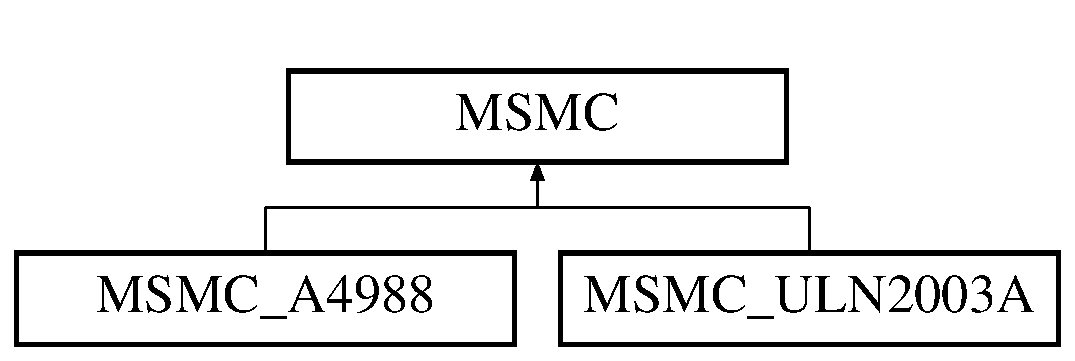
\includegraphics[height=2.000000cm]{class_m_s_m_c}
\end{center}
\end{figure}
\subsection*{Public Member Functions}
\begin{DoxyCompactItemize}
\item 
virtual void \hyperlink{class_m_s_m_c_a62615946a227d18ea3fc2f1329688d1f}{forward} (uint32\+\_\+t, uint32\+\_\+t)
\item 
virtual void \hyperlink{class_m_s_m_c_a389bfe7f7d05083cb4e95d73128c1c87}{backward} (uint32\+\_\+t, uint32\+\_\+t)
\item 
virtual void \hyperlink{class_m_s_m_c_a065e48c8e8f3b513bf6694e8eb1b28d5}{speed} (uint32\+\_\+t)
\item 
virtual void \hyperlink{class_m_s_m_c_a0b44d0a659550ba754bf9212294ba6d5}{stop} ()
\item 
virtual void \hyperlink{class_m_s_m_c_a9c45f1547467b43209c7a271604e7c85}{pause} ()
\item 
virtual void \hyperlink{class_m_s_m_c_ae09c870a71121c7cc9f060b6299a425b}{restart} ()
\item 
virtual void \hyperlink{class_m_s_m_c_a85bd4abf542aecdf24bb90b9ea2a47e9}{set\+Mode} (uint8\+\_\+t)
\item 
virtual uint8\+\_\+t \hyperlink{class_m_s_m_c_a5a1c4ee3498360946cc8e8d39436d0e3}{get\+Mode} ()
\item 
virtual int8\+\_\+t \hyperlink{class_m_s_m_c_a97ba8d296c68e2bb2a3b3eebe047dca8}{get\+Dir} ()
\item 
virtual uint32\+\_\+t \hyperlink{class_m_s_m_c_a365b393eba0c9d7d42e37d32db6c00b7}{get\+Steps} ()
\item 
virtual boolean \hyperlink{class_m_s_m_c_a2c379d628edbca2d36e3588b39bf6b98}{update} ()
\end{DoxyCompactItemize}


\subsection{Detailed Description}
The multi stepper motor control interface. 

\subsection{Member Function Documentation}
\hypertarget{class_m_s_m_c_a389bfe7f7d05083cb4e95d73128c1c87}{\index{M\+S\+M\+C@{M\+S\+M\+C}!backward@{backward}}
\index{backward@{backward}!M\+S\+M\+C@{M\+S\+M\+C}}
\subsubsection[{backward}]{\setlength{\rightskip}{0pt plus 5cm}virtual void M\+S\+M\+C\+::backward (
\begin{DoxyParamCaption}
\item[{uint32\+\_\+t}]{, }
\item[{uint32\+\_\+t}]{}
\end{DoxyParamCaption}
)\hspace{0.3cm}{\ttfamily [virtual]}}}\label{class_m_s_m_c_a389bfe7f7d05083cb4e95d73128c1c87}


Reimplemented in \hyperlink{class_m_s_m_c___u_l_n2003_a_ac46e6ec6345f95b534079bcf2920885e}{M\+S\+M\+C\+\_\+\+U\+L\+N2003\+A}, and \hyperlink{class_m_s_m_c___a4988_a836bed9e28e723ead2a94446bb704869}{M\+S\+M\+C\+\_\+\+A4988}.

\hypertarget{class_m_s_m_c_a62615946a227d18ea3fc2f1329688d1f}{\index{M\+S\+M\+C@{M\+S\+M\+C}!forward@{forward}}
\index{forward@{forward}!M\+S\+M\+C@{M\+S\+M\+C}}
\subsubsection[{forward}]{\setlength{\rightskip}{0pt plus 5cm}virtual void M\+S\+M\+C\+::forward (
\begin{DoxyParamCaption}
\item[{uint32\+\_\+t}]{, }
\item[{uint32\+\_\+t}]{}
\end{DoxyParamCaption}
)\hspace{0.3cm}{\ttfamily [virtual]}}}\label{class_m_s_m_c_a62615946a227d18ea3fc2f1329688d1f}


Reimplemented in \hyperlink{class_m_s_m_c___u_l_n2003_a_a9657492f948a75472b311bc0b823899f}{M\+S\+M\+C\+\_\+\+U\+L\+N2003\+A}, and \hyperlink{class_m_s_m_c___a4988_a9acdbabf546656a6436e89579e8fcfca}{M\+S\+M\+C\+\_\+\+A4988}.

\hypertarget{class_m_s_m_c_a97ba8d296c68e2bb2a3b3eebe047dca8}{\index{M\+S\+M\+C@{M\+S\+M\+C}!get\+Dir@{get\+Dir}}
\index{get\+Dir@{get\+Dir}!M\+S\+M\+C@{M\+S\+M\+C}}
\subsubsection[{get\+Dir}]{\setlength{\rightskip}{0pt plus 5cm}virtual int8\+\_\+t M\+S\+M\+C\+::get\+Dir (
\begin{DoxyParamCaption}
{}
\end{DoxyParamCaption}
)\hspace{0.3cm}{\ttfamily [virtual]}}}\label{class_m_s_m_c_a97ba8d296c68e2bb2a3b3eebe047dca8}


Reimplemented in \hyperlink{class_m_s_m_c___a4988_acf7598266c1ced18507d43f811c98db9}{M\+S\+M\+C\+\_\+\+A4988}.

\hypertarget{class_m_s_m_c_a5a1c4ee3498360946cc8e8d39436d0e3}{\index{M\+S\+M\+C@{M\+S\+M\+C}!get\+Mode@{get\+Mode}}
\index{get\+Mode@{get\+Mode}!M\+S\+M\+C@{M\+S\+M\+C}}
\subsubsection[{get\+Mode}]{\setlength{\rightskip}{0pt plus 5cm}virtual uint8\+\_\+t M\+S\+M\+C\+::get\+Mode (
\begin{DoxyParamCaption}
{}
\end{DoxyParamCaption}
)\hspace{0.3cm}{\ttfamily [virtual]}}}\label{class_m_s_m_c_a5a1c4ee3498360946cc8e8d39436d0e3}


Reimplemented in \hyperlink{class_m_s_m_c___u_l_n2003_a_a84cbd656e77e789af5cb34df147589a3}{M\+S\+M\+C\+\_\+\+U\+L\+N2003\+A}, and \hyperlink{class_m_s_m_c___a4988_ab0004d7e88ada9fc74b21fd5886bdb54}{M\+S\+M\+C\+\_\+\+A4988}.

\hypertarget{class_m_s_m_c_a365b393eba0c9d7d42e37d32db6c00b7}{\index{M\+S\+M\+C@{M\+S\+M\+C}!get\+Steps@{get\+Steps}}
\index{get\+Steps@{get\+Steps}!M\+S\+M\+C@{M\+S\+M\+C}}
\subsubsection[{get\+Steps}]{\setlength{\rightskip}{0pt plus 5cm}virtual uint32\+\_\+t M\+S\+M\+C\+::get\+Steps (
\begin{DoxyParamCaption}
{}
\end{DoxyParamCaption}
)\hspace{0.3cm}{\ttfamily [virtual]}}}\label{class_m_s_m_c_a365b393eba0c9d7d42e37d32db6c00b7}


Reimplemented in \hyperlink{class_m_s_m_c___u_l_n2003_a_a06c602281da9eebbd38dc4151c137609}{M\+S\+M\+C\+\_\+\+U\+L\+N2003\+A}, and \hyperlink{class_m_s_m_c___a4988_ab097e238a4a8c905e478ecff23907059}{M\+S\+M\+C\+\_\+\+A4988}.

\hypertarget{class_m_s_m_c_a9c45f1547467b43209c7a271604e7c85}{\index{M\+S\+M\+C@{M\+S\+M\+C}!pause@{pause}}
\index{pause@{pause}!M\+S\+M\+C@{M\+S\+M\+C}}
\subsubsection[{pause}]{\setlength{\rightskip}{0pt plus 5cm}virtual void M\+S\+M\+C\+::pause (
\begin{DoxyParamCaption}
{}
\end{DoxyParamCaption}
)\hspace{0.3cm}{\ttfamily [virtual]}}}\label{class_m_s_m_c_a9c45f1547467b43209c7a271604e7c85}


Reimplemented in \hyperlink{class_m_s_m_c___u_l_n2003_a_aa1d3444465d59ca6c87f05f565dde4a2}{M\+S\+M\+C\+\_\+\+U\+L\+N2003\+A}, and \hyperlink{class_m_s_m_c___a4988_a321bc53bae537a0318910819a6a1a7d5}{M\+S\+M\+C\+\_\+\+A4988}.

\hypertarget{class_m_s_m_c_ae09c870a71121c7cc9f060b6299a425b}{\index{M\+S\+M\+C@{M\+S\+M\+C}!restart@{restart}}
\index{restart@{restart}!M\+S\+M\+C@{M\+S\+M\+C}}
\subsubsection[{restart}]{\setlength{\rightskip}{0pt plus 5cm}virtual void M\+S\+M\+C\+::restart (
\begin{DoxyParamCaption}
{}
\end{DoxyParamCaption}
)\hspace{0.3cm}{\ttfamily [virtual]}}}\label{class_m_s_m_c_ae09c870a71121c7cc9f060b6299a425b}


Reimplemented in \hyperlink{class_m_s_m_c___u_l_n2003_a_a19853d77f81c521091a55996899c1784}{M\+S\+M\+C\+\_\+\+U\+L\+N2003\+A}, and \hyperlink{class_m_s_m_c___a4988_add93aa459190c6edb3551495e75aaded}{M\+S\+M\+C\+\_\+\+A4988}.

\hypertarget{class_m_s_m_c_a85bd4abf542aecdf24bb90b9ea2a47e9}{\index{M\+S\+M\+C@{M\+S\+M\+C}!set\+Mode@{set\+Mode}}
\index{set\+Mode@{set\+Mode}!M\+S\+M\+C@{M\+S\+M\+C}}
\subsubsection[{set\+Mode}]{\setlength{\rightskip}{0pt plus 5cm}virtual void M\+S\+M\+C\+::set\+Mode (
\begin{DoxyParamCaption}
\item[{uint8\+\_\+t}]{}
\end{DoxyParamCaption}
)\hspace{0.3cm}{\ttfamily [virtual]}}}\label{class_m_s_m_c_a85bd4abf542aecdf24bb90b9ea2a47e9}


Reimplemented in \hyperlink{class_m_s_m_c___u_l_n2003_a_a8a7f8b7e0048b3a03c87bd830d4a455f}{M\+S\+M\+C\+\_\+\+U\+L\+N2003\+A}, and \hyperlink{class_m_s_m_c___a4988_aa4b96442c0e7d68715c2322f5bdce782}{M\+S\+M\+C\+\_\+\+A4988}.

\hypertarget{class_m_s_m_c_a065e48c8e8f3b513bf6694e8eb1b28d5}{\index{M\+S\+M\+C@{M\+S\+M\+C}!speed@{speed}}
\index{speed@{speed}!M\+S\+M\+C@{M\+S\+M\+C}}
\subsubsection[{speed}]{\setlength{\rightskip}{0pt plus 5cm}virtual void M\+S\+M\+C\+::speed (
\begin{DoxyParamCaption}
\item[{uint32\+\_\+t}]{}
\end{DoxyParamCaption}
)\hspace{0.3cm}{\ttfamily [virtual]}}}\label{class_m_s_m_c_a065e48c8e8f3b513bf6694e8eb1b28d5}


Reimplemented in \hyperlink{class_m_s_m_c___u_l_n2003_a_ad8df164c90b2205fb65c796632889f82}{M\+S\+M\+C\+\_\+\+U\+L\+N2003\+A}, and \hyperlink{class_m_s_m_c___a4988_a6f9d236dc619342d16457aa029faeed9}{M\+S\+M\+C\+\_\+\+A4988}.

\hypertarget{class_m_s_m_c_a0b44d0a659550ba754bf9212294ba6d5}{\index{M\+S\+M\+C@{M\+S\+M\+C}!stop@{stop}}
\index{stop@{stop}!M\+S\+M\+C@{M\+S\+M\+C}}
\subsubsection[{stop}]{\setlength{\rightskip}{0pt plus 5cm}virtual void M\+S\+M\+C\+::stop (
\begin{DoxyParamCaption}
{}
\end{DoxyParamCaption}
)\hspace{0.3cm}{\ttfamily [virtual]}}}\label{class_m_s_m_c_a0b44d0a659550ba754bf9212294ba6d5}


Reimplemented in \hyperlink{class_m_s_m_c___u_l_n2003_a_aba5e18f20f31fd4d6e71f50821dfeee5}{M\+S\+M\+C\+\_\+\+U\+L\+N2003\+A}, and \hyperlink{class_m_s_m_c___a4988_a4038481ce6b8131ea22d5e0d331ca6c7}{M\+S\+M\+C\+\_\+\+A4988}.

\hypertarget{class_m_s_m_c_a2c379d628edbca2d36e3588b39bf6b98}{\index{M\+S\+M\+C@{M\+S\+M\+C}!update@{update}}
\index{update@{update}!M\+S\+M\+C@{M\+S\+M\+C}}
\subsubsection[{update}]{\setlength{\rightskip}{0pt plus 5cm}virtual boolean M\+S\+M\+C\+::update (
\begin{DoxyParamCaption}
{}
\end{DoxyParamCaption}
)\hspace{0.3cm}{\ttfamily [virtual]}}}\label{class_m_s_m_c_a2c379d628edbca2d36e3588b39bf6b98}


Reimplemented in \hyperlink{class_m_s_m_c___u_l_n2003_a_acdf6b6224352a90146e67ee9837d0a6f}{M\+S\+M\+C\+\_\+\+U\+L\+N2003\+A}, and \hyperlink{class_m_s_m_c___a4988_a409bea28b42827c8bd7d5e5e318af21d}{M\+S\+M\+C\+\_\+\+A4988}.



The documentation for this class was generated from the following file\+:\begin{DoxyCompactItemize}
\item 
\hyperlink{_m_s_m_c_8h}{M\+S\+M\+C.\+h}\end{DoxyCompactItemize}

\hypertarget{class_m_s_m_c___a4988}{\section{M\+S\+M\+C\+\_\+\+A4988 Class Reference}
\label{class_m_s_m_c___a4988}\index{M\+S\+M\+C\+\_\+\+A4988@{M\+S\+M\+C\+\_\+\+A4988}}
}


Multi Stepper Motor Control with A4988.  




{\ttfamily \#include $<$M\+S\+M\+C\+\_\+\+A4988.\+h$>$}

Inheritance diagram for M\+S\+M\+C\+\_\+\+A4988\+:\begin{figure}[H]
\begin{center}
\leavevmode
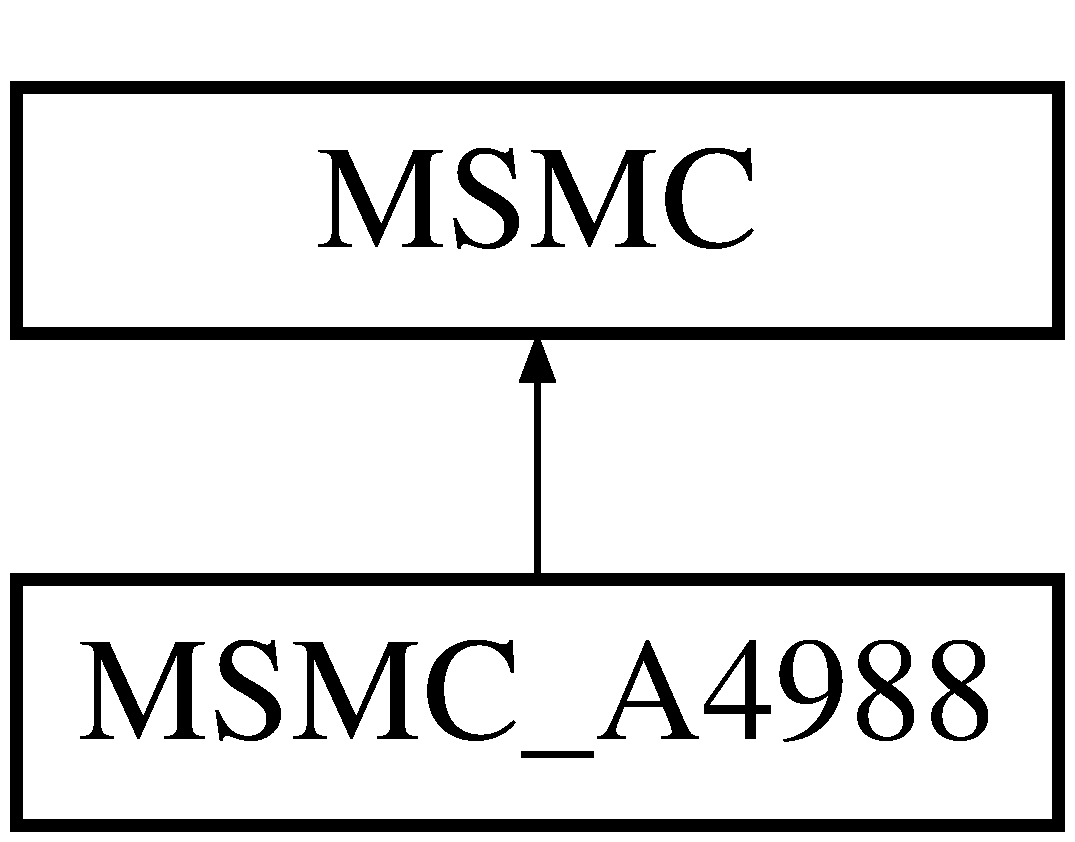
\includegraphics[height=2.000000cm]{class_m_s_m_c___a4988}
\end{center}
\end{figure}
\subsection*{Public Member Functions}
\begin{DoxyCompactItemize}
\item 
\hyperlink{class_m_s_m_c___a4988_a3ea9fb71304c6a21695947fde680ee48}{M\+S\+M\+C\+\_\+\+A4988} ()
\begin{DoxyCompactList}\small\item\em Default constructor. \end{DoxyCompactList}\item 
\hyperlink{class_m_s_m_c___a4988_af2633e82e29d622a4fb5b5f8f6b77446}{M\+S\+M\+C\+\_\+\+A4988} (uint8\+\_\+t pst, uint8\+\_\+t pdr, uint8\+\_\+t pen)
\begin{DoxyCompactList}\small\item\em Constructor. \end{DoxyCompactList}\item 
void \hyperlink{class_m_s_m_c___a4988_a9acdbabf546656a6436e89579e8fcfca}{forward} (uint32\+\_\+t st, uint32\+\_\+t sp)
\begin{DoxyCompactList}\small\item\em Configure the motor to move forward. \end{DoxyCompactList}\item 
void \hyperlink{class_m_s_m_c___a4988_a836bed9e28e723ead2a94446bb704869}{backward} (uint32\+\_\+t st, uint32\+\_\+t sp)
\begin{DoxyCompactList}\small\item\em Configure the motor to move backward. \end{DoxyCompactList}\item 
void \hyperlink{class_m_s_m_c___a4988_a7aa6ddff4b561e47f09e4726b160294b}{set\+Pins} (uint8\+\_\+t pst, uint8\+\_\+t pdr, uint8\+\_\+t pen)
\begin{DoxyCompactList}\small\item\em Set up the pins attached to the A4988. \end{DoxyCompactList}\item 
void \hyperlink{class_m_s_m_c___a4988_aa4b96442c0e7d68715c2322f5bdce782}{set\+Mode} (uint8\+\_\+t mod)
\begin{DoxyCompactList}\small\item\em Set up the control mode. \end{DoxyCompactList}\item 
uint8\+\_\+t \hyperlink{class_m_s_m_c___a4988_ab0004d7e88ada9fc74b21fd5886bdb54}{get\+Mode} ()
\begin{DoxyCompactList}\small\item\em Return the operative mode of the controller. \end{DoxyCompactList}\item 
void \hyperlink{class_m_s_m_c___a4988_a6f9d236dc619342d16457aa029faeed9}{speed} (uint32\+\_\+t sp)
\begin{DoxyCompactList}\small\item\em Change the delay between each step. \end{DoxyCompactList}\item 
void \hyperlink{class_m_s_m_c___a4988_a4038481ce6b8131ea22d5e0d331ca6c7}{stop} ()
\begin{DoxyCompactList}\small\item\em Stop any motion. \end{DoxyCompactList}\item 
int32\+\_\+t \hyperlink{class_m_s_m_c___a4988_a1f408597bc1daf8bb5e563d54bf32cdd}{update} ()
\begin{DoxyCompactList}\small\item\em Perform the motion of the motor. \end{DoxyCompactList}\end{DoxyCompactItemize}
\subsection*{Private Member Functions}
\begin{DoxyCompactItemize}
\item 
void \hyperlink{class_m_s_m_c___a4988_ac177dd03f28d347cfa6212bc54394027}{one\+\_\+step\+\_\+drive} (boolean v)
\item 
void \hyperlink{class_m_s_m_c___a4988_ab9bd155f40ee777f17d1c4b1a702a60a}{set\+Direction} ()
\begin{DoxyCompactList}\small\item\em It drives the direction pin. \end{DoxyCompactList}\item 
void \hyperlink{class_m_s_m_c___a4988_a1157e26b461a3689558cd205880ef3b9}{enable} ()
\begin{DoxyCompactList}\small\item\em Enable the F\+E\+Ts of the A4988 that control the coils of the motor, the pin is low active.. \end{DoxyCompactList}\item 
void \hyperlink{class_m_s_m_c___a4988_a525c9313ee313d9c6316fc743b7b4ae0}{disable} ()
\begin{DoxyCompactList}\small\item\em Disable the F\+E\+Ts of the A4988 that control the coils of the motor. \end{DoxyCompactList}\end{DoxyCompactItemize}
\subsection*{Private Attributes}
\begin{DoxyCompactItemize}
\item 
uint8\+\_\+t \hyperlink{class_m_s_m_c___a4988_a2ea61398ce88d1ee627b409a5965b478}{pin\+\_\+step}
\begin{DoxyCompactList}\small\item\em The pin controls the step. \end{DoxyCompactList}\item 
uint8\+\_\+t \hyperlink{class_m_s_m_c___a4988_a2bc9676a272bcd6604aaf8b08ac07109}{pin\+\_\+dir}
\begin{DoxyCompactList}\small\item\em The pin controls the direction. \end{DoxyCompactList}\item 
uint8\+\_\+t \hyperlink{class_m_s_m_c___a4988_a822c3db98367f3e60347a13d1d16170b}{pin\+\_\+enable}
\begin{DoxyCompactList}\small\item\em The pin controls the enable pin of the A4988. \end{DoxyCompactList}\item 
uint32\+\_\+t \hyperlink{class_m_s_m_c___a4988_a6453efb52d22739962c05b0d03f65aa7}{spd}
\begin{DoxyCompactList}\small\item\em The delay between two steps in microseconds. \end{DoxyCompactList}\item 
uint32\+\_\+t \hyperlink{class_m_s_m_c___a4988_aa85fc95facc940db652cd2f545f033cd}{steps}
\begin{DoxyCompactList}\small\item\em The number of steps until the motion ends. \end{DoxyCompactList}\item 
uint32\+\_\+t \hyperlink{class_m_s_m_c___a4988_aa7de83eb15a9f82533b898146921939b}{tot\+\_\+steps}
\begin{DoxyCompactList}\small\item\em The total steps set by \hyperlink{class_m_s_m_c___a4988_a9acdbabf546656a6436e89579e8fcfca}{forward()} and \hyperlink{class_m_s_m_c___a4988_a836bed9e28e723ead2a94446bb704869}{backward()}. \end{DoxyCompactList}\item 
uint32\+\_\+t \hyperlink{class_m_s_m_c___a4988_a60ff02342382a71526d14fb9e51ddc2a}{old\+\_\+time}
\begin{DoxyCompactList}\small\item\em The time value in microseconds set during the last step. \end{DoxyCompactList}\item 
int8\+\_\+t \hyperlink{class_m_s_m_c___a4988_a887a3d29966bdfc0d920d339b83e5346}{dir}
\begin{DoxyCompactList}\small\item\em Specify the direction of the motor\+: -\/1 backward, 1 forward, 0 all pin out L\+O\+W. \end{DoxyCompactList}\item 
boolean \hyperlink{class_m_s_m_c___a4988_a86ef4c886ee6c7ed6fa87e27c0a7a9ea}{m\+\_\+ready}
\begin{DoxyCompactList}\small\item\em True if the motor is ready to take a new command\+: \hyperlink{class_m_s_m_c___a4988_a9acdbabf546656a6436e89579e8fcfca}{forward(uint32\+\_\+t, uint32\+\_\+t)} or \hyperlink{class_m_s_m_c___a4988_a836bed9e28e723ead2a94446bb704869}{backward(uint32\+\_\+t, uint32\+\_\+t)}. \end{DoxyCompactList}\item 
boolean \hyperlink{class_m_s_m_c___a4988_a1ec86b6286b8827eca6d5703a02f65fd}{step\+\_\+pin\+\_\+val}
\begin{DoxyCompactList}\small\item\em The value of the pin that drives the step advance. \end{DoxyCompactList}\item 
uint8\+\_\+t \hyperlink{class_m_s_m_c___a4988_a819ff8eed30ef364c710a1fb1371d18e}{control\+\_\+mode}
\begin{DoxyCompactList}\small\item\em Specify the control mode of the motor\+: 0 full step, 1 half step, 2 quarter step, 3 eighth step and 4 sixteenth step. \end{DoxyCompactList}\end{DoxyCompactItemize}


\subsection{Detailed Description}
Multi Stepper Motor Control with A4988. 

The class allows the contemporary control of multi stepper motors using the I\+Cs A4988. After the motor setup, you can drive the motor forward and backward, specifying the number of steps and the delay in microseconds between two consecutive steps. The function update performs the effective motor motion, it must be call in the main loop and, if the delay is expired, the function moves the motor of one step. \begin{DoxyAuthor}{Author}
Francesco Giurlanda 
\end{DoxyAuthor}


\subsection{Constructor \& Destructor Documentation}
\hypertarget{class_m_s_m_c___a4988_a3ea9fb71304c6a21695947fde680ee48}{\index{M\+S\+M\+C\+\_\+\+A4988@{M\+S\+M\+C\+\_\+\+A4988}!M\+S\+M\+C\+\_\+\+A4988@{M\+S\+M\+C\+\_\+\+A4988}}
\index{M\+S\+M\+C\+\_\+\+A4988@{M\+S\+M\+C\+\_\+\+A4988}!M\+S\+M\+C\+\_\+\+A4988@{M\+S\+M\+C\+\_\+\+A4988}}
\subsubsection[{M\+S\+M\+C\+\_\+\+A4988}]{\setlength{\rightskip}{0pt plus 5cm}M\+S\+M\+C\+\_\+\+A4988\+::\+M\+S\+M\+C\+\_\+\+A4988 (
\begin{DoxyParamCaption}
{}
\end{DoxyParamCaption}
)}}\label{class_m_s_m_c___a4988_a3ea9fb71304c6a21695947fde680ee48}


Default constructor. 

\hypertarget{class_m_s_m_c___a4988_af2633e82e29d622a4fb5b5f8f6b77446}{\index{M\+S\+M\+C\+\_\+\+A4988@{M\+S\+M\+C\+\_\+\+A4988}!M\+S\+M\+C\+\_\+\+A4988@{M\+S\+M\+C\+\_\+\+A4988}}
\index{M\+S\+M\+C\+\_\+\+A4988@{M\+S\+M\+C\+\_\+\+A4988}!M\+S\+M\+C\+\_\+\+A4988@{M\+S\+M\+C\+\_\+\+A4988}}
\subsubsection[{M\+S\+M\+C\+\_\+\+A4988}]{\setlength{\rightskip}{0pt plus 5cm}M\+S\+M\+C\+\_\+\+A4988\+::\+M\+S\+M\+C\+\_\+\+A4988 (
\begin{DoxyParamCaption}
\item[{uint8\+\_\+t}]{pst, }
\item[{uint8\+\_\+t}]{pdr, }
\item[{uint8\+\_\+t}]{pen}
\end{DoxyParamCaption}
)}}\label{class_m_s_m_c___a4988_af2633e82e29d622a4fb5b5f8f6b77446}


Constructor. 


\begin{DoxyParams}{Parameters}
{\em pst} & The number of the pin which is attached to the step control pin of the A4988. \\
\hline
{\em pdr} & The number of the pin which is attached to the direction control pin of the A4988. \\
\hline
{\em pen} & The number of the pin which is attached to the enable pin of the A4988. \\
\hline
\end{DoxyParams}


\subsection{Member Function Documentation}
\hypertarget{class_m_s_m_c___a4988_a836bed9e28e723ead2a94446bb704869}{\index{M\+S\+M\+C\+\_\+\+A4988@{M\+S\+M\+C\+\_\+\+A4988}!backward@{backward}}
\index{backward@{backward}!M\+S\+M\+C\+\_\+\+A4988@{M\+S\+M\+C\+\_\+\+A4988}}
\subsubsection[{backward}]{\setlength{\rightskip}{0pt plus 5cm}void M\+S\+M\+C\+\_\+\+A4988\+::backward (
\begin{DoxyParamCaption}
\item[{uint32\+\_\+t}]{st, }
\item[{uint32\+\_\+t}]{sp}
\end{DoxyParamCaption}
)\hspace{0.3cm}{\ttfamily [virtual]}}}\label{class_m_s_m_c___a4988_a836bed9e28e723ead2a94446bb704869}


Configure the motor to move backward. 

The function moves backward the motor of a number of steps with a specified delay between each step 
\begin{DoxyParams}{Parameters}
{\em st} & The number of steps \\
\hline
{\em sp} & The delay between the steps in microseconds \\
\hline
\end{DoxyParams}
\begin{DoxySeeAlso}{See also}
\hyperlink{class_m_s_m_c___a4988_a9acdbabf546656a6436e89579e8fcfca}{forward(uint32\+\_\+t, uint32\+\_\+t)} 
\end{DoxySeeAlso}


Reimplemented from \hyperlink{class_m_s_m_c_a389bfe7f7d05083cb4e95d73128c1c87}{M\+S\+M\+C}.

\hypertarget{class_m_s_m_c___a4988_a525c9313ee313d9c6316fc743b7b4ae0}{\index{M\+S\+M\+C\+\_\+\+A4988@{M\+S\+M\+C\+\_\+\+A4988}!disable@{disable}}
\index{disable@{disable}!M\+S\+M\+C\+\_\+\+A4988@{M\+S\+M\+C\+\_\+\+A4988}}
\subsubsection[{disable}]{\setlength{\rightskip}{0pt plus 5cm}void M\+S\+M\+C\+\_\+\+A4988\+::disable (
\begin{DoxyParamCaption}
{}
\end{DoxyParamCaption}
)\hspace{0.3cm}{\ttfamily [private]}}}\label{class_m_s_m_c___a4988_a525c9313ee313d9c6316fc743b7b4ae0}


Disable the F\+E\+Ts of the A4988 that control the coils of the motor. 

\hypertarget{class_m_s_m_c___a4988_a1157e26b461a3689558cd205880ef3b9}{\index{M\+S\+M\+C\+\_\+\+A4988@{M\+S\+M\+C\+\_\+\+A4988}!enable@{enable}}
\index{enable@{enable}!M\+S\+M\+C\+\_\+\+A4988@{M\+S\+M\+C\+\_\+\+A4988}}
\subsubsection[{enable}]{\setlength{\rightskip}{0pt plus 5cm}void M\+S\+M\+C\+\_\+\+A4988\+::enable (
\begin{DoxyParamCaption}
{}
\end{DoxyParamCaption}
)\hspace{0.3cm}{\ttfamily [private]}}}\label{class_m_s_m_c___a4988_a1157e26b461a3689558cd205880ef3b9}


Enable the F\+E\+Ts of the A4988 that control the coils of the motor, the pin is low active.. 

\hypertarget{class_m_s_m_c___a4988_a9acdbabf546656a6436e89579e8fcfca}{\index{M\+S\+M\+C\+\_\+\+A4988@{M\+S\+M\+C\+\_\+\+A4988}!forward@{forward}}
\index{forward@{forward}!M\+S\+M\+C\+\_\+\+A4988@{M\+S\+M\+C\+\_\+\+A4988}}
\subsubsection[{forward}]{\setlength{\rightskip}{0pt plus 5cm}void M\+S\+M\+C\+\_\+\+A4988\+::forward (
\begin{DoxyParamCaption}
\item[{uint32\+\_\+t}]{st, }
\item[{uint32\+\_\+t}]{sp}
\end{DoxyParamCaption}
)\hspace{0.3cm}{\ttfamily [virtual]}}}\label{class_m_s_m_c___a4988_a9acdbabf546656a6436e89579e8fcfca}


Configure the motor to move forward. 

The function moves forward the motor of a number of steps with a specified delay between each step 
\begin{DoxyParams}{Parameters}
{\em st} & The number of steps \\
\hline
{\em sp} & The delay between the steps in microseconds \\
\hline
\end{DoxyParams}
\begin{DoxySeeAlso}{See also}
\hyperlink{class_m_s_m_c___a4988_a836bed9e28e723ead2a94446bb704869}{backward(uint32\+\_\+t, uint32\+\_\+t)} 
\end{DoxySeeAlso}


Reimplemented from \hyperlink{class_m_s_m_c_a62615946a227d18ea3fc2f1329688d1f}{M\+S\+M\+C}.

\hypertarget{class_m_s_m_c___a4988_ab0004d7e88ada9fc74b21fd5886bdb54}{\index{M\+S\+M\+C\+\_\+\+A4988@{M\+S\+M\+C\+\_\+\+A4988}!get\+Mode@{get\+Mode}}
\index{get\+Mode@{get\+Mode}!M\+S\+M\+C\+\_\+\+A4988@{M\+S\+M\+C\+\_\+\+A4988}}
\subsubsection[{get\+Mode}]{\setlength{\rightskip}{0pt plus 5cm}uint8\+\_\+t M\+S\+M\+C\+\_\+\+A4988\+::get\+Mode (
\begin{DoxyParamCaption}
{}
\end{DoxyParamCaption}
)\hspace{0.3cm}{\ttfamily [virtual]}}}\label{class_m_s_m_c___a4988_ab0004d7e88ada9fc74b21fd5886bdb54}


Return the operative mode of the controller. 

\begin{DoxyReturn}{Returns}
An int that identifies the operative mode\+: \hyperlink{_m_s_m_c___u_l_n2003_a_8h_a65ffcc85557e6fc00e865d67e20f720e}{F\+U\+L\+L\+\_\+\+S\+T\+E\+P}, \hyperlink{_m_s_m_c___u_l_n2003_a_8h_af078dda416ad0114e9c81a6c36c0801f}{H\+A\+L\+F\+\_\+\+S\+T\+E\+P}, \hyperlink{_m_s_m_c___a4988_8h_a5bf980ea8dd6df6a0271f6d30d66931b}{Q\+U\+A\+R\+T\+E\+R\+\_\+\+S\+T\+E\+P}, \hyperlink{_m_s_m_c___a4988_8h_ac3f074c3e3b349fc9f6487a9d9a77399}{E\+I\+G\+H\+T\+H\+\_\+\+S\+T\+E\+P} and \hyperlink{_m_s_m_c___a4988_8h_a8493986c329fb4bfde621461028b3a31}{S\+I\+X\+T\+E\+E\+N\+T\+H\+\_\+\+S\+T\+E\+P} 
\end{DoxyReturn}


Reimplemented from \hyperlink{class_m_s_m_c_a5a1c4ee3498360946cc8e8d39436d0e3}{M\+S\+M\+C}.

\hypertarget{class_m_s_m_c___a4988_ac177dd03f28d347cfa6212bc54394027}{\index{M\+S\+M\+C\+\_\+\+A4988@{M\+S\+M\+C\+\_\+\+A4988}!one\+\_\+step\+\_\+drive@{one\+\_\+step\+\_\+drive}}
\index{one\+\_\+step\+\_\+drive@{one\+\_\+step\+\_\+drive}!M\+S\+M\+C\+\_\+\+A4988@{M\+S\+M\+C\+\_\+\+A4988}}
\subsubsection[{one\+\_\+step\+\_\+drive}]{\setlength{\rightskip}{0pt plus 5cm}void M\+S\+M\+C\+\_\+\+A4988\+::one\+\_\+step\+\_\+drive (
\begin{DoxyParamCaption}
\item[{boolean}]{v}
\end{DoxyParamCaption}
)\hspace{0.3cm}{\ttfamily [private]}}}\label{class_m_s_m_c___a4988_ac177dd03f28d347cfa6212bc54394027}
\hypertarget{class_m_s_m_c___a4988_ab9bd155f40ee777f17d1c4b1a702a60a}{\index{M\+S\+M\+C\+\_\+\+A4988@{M\+S\+M\+C\+\_\+\+A4988}!set\+Direction@{set\+Direction}}
\index{set\+Direction@{set\+Direction}!M\+S\+M\+C\+\_\+\+A4988@{M\+S\+M\+C\+\_\+\+A4988}}
\subsubsection[{set\+Direction}]{\setlength{\rightskip}{0pt plus 5cm}void M\+S\+M\+C\+\_\+\+A4988\+::set\+Direction (
\begin{DoxyParamCaption}
{}
\end{DoxyParamCaption}
)\hspace{0.3cm}{\ttfamily [private]}}}\label{class_m_s_m_c___a4988_ab9bd155f40ee777f17d1c4b1a702a60a}


It drives the direction pin. 

\hypertarget{class_m_s_m_c___a4988_aa4b96442c0e7d68715c2322f5bdce782}{\index{M\+S\+M\+C\+\_\+\+A4988@{M\+S\+M\+C\+\_\+\+A4988}!set\+Mode@{set\+Mode}}
\index{set\+Mode@{set\+Mode}!M\+S\+M\+C\+\_\+\+A4988@{M\+S\+M\+C\+\_\+\+A4988}}
\subsubsection[{set\+Mode}]{\setlength{\rightskip}{0pt plus 5cm}void M\+S\+M\+C\+\_\+\+A4988\+::set\+Mode (
\begin{DoxyParamCaption}
\item[{uint8\+\_\+t}]{mod}
\end{DoxyParamCaption}
)\hspace{0.3cm}{\ttfamily [virtual]}}}\label{class_m_s_m_c___a4988_aa4b96442c0e7d68715c2322f5bdce782}


Set up the control mode. 


\begin{DoxyParams}{Parameters}
{\em mod} & The mode used to control the motor. You can use the following macros\+:
\begin{DoxyItemize}
\item \hyperlink{_m_s_m_c___u_l_n2003_a_8h_a65ffcc85557e6fc00e865d67e20f720e}{F\+U\+L\+L\+\_\+\+S\+T\+E\+P}
\item \hyperlink{_m_s_m_c___u_l_n2003_a_8h_af078dda416ad0114e9c81a6c36c0801f}{H\+A\+L\+F\+\_\+\+S\+T\+E\+P}
\item \hyperlink{_m_s_m_c___a4988_8h_a5bf980ea8dd6df6a0271f6d30d66931b}{Q\+U\+A\+R\+T\+E\+R\+\_\+\+S\+T\+E\+P}
\item \hyperlink{_m_s_m_c___a4988_8h_ac3f074c3e3b349fc9f6487a9d9a77399}{E\+I\+G\+H\+T\+H\+\_\+\+S\+T\+E\+P}
\item \hyperlink{_m_s_m_c___a4988_8h_a8493986c329fb4bfde621461028b3a31}{S\+I\+X\+T\+E\+E\+N\+T\+H\+\_\+\+S\+T\+E\+P} 
\end{DoxyItemize}\\
\hline
\end{DoxyParams}


Reimplemented from \hyperlink{class_m_s_m_c_a85bd4abf542aecdf24bb90b9ea2a47e9}{M\+S\+M\+C}.

\hypertarget{class_m_s_m_c___a4988_a7aa6ddff4b561e47f09e4726b160294b}{\index{M\+S\+M\+C\+\_\+\+A4988@{M\+S\+M\+C\+\_\+\+A4988}!set\+Pins@{set\+Pins}}
\index{set\+Pins@{set\+Pins}!M\+S\+M\+C\+\_\+\+A4988@{M\+S\+M\+C\+\_\+\+A4988}}
\subsubsection[{set\+Pins}]{\setlength{\rightskip}{0pt plus 5cm}void M\+S\+M\+C\+\_\+\+A4988\+::set\+Pins (
\begin{DoxyParamCaption}
\item[{uint8\+\_\+t}]{pst, }
\item[{uint8\+\_\+t}]{pdr, }
\item[{uint8\+\_\+t}]{pen}
\end{DoxyParamCaption}
)}}\label{class_m_s_m_c___a4988_a7aa6ddff4b561e47f09e4726b160294b}


Set up the pins attached to the A4988. 


\begin{DoxyParams}{Parameters}
{\em pst} & The number of the pin which is attached to the step control pin of the A4988. \\
\hline
{\em pdr} & The number of the pin which is attached to the direction control pin of the A4988. \\
\hline
{\em pen} & The number of the pin which is attached to the enable pin of the A4988. \\
\hline
\end{DoxyParams}
\hypertarget{class_m_s_m_c___a4988_a6f9d236dc619342d16457aa029faeed9}{\index{M\+S\+M\+C\+\_\+\+A4988@{M\+S\+M\+C\+\_\+\+A4988}!speed@{speed}}
\index{speed@{speed}!M\+S\+M\+C\+\_\+\+A4988@{M\+S\+M\+C\+\_\+\+A4988}}
\subsubsection[{speed}]{\setlength{\rightskip}{0pt plus 5cm}void M\+S\+M\+C\+\_\+\+A4988\+::speed (
\begin{DoxyParamCaption}
\item[{uint32\+\_\+t}]{sp}
\end{DoxyParamCaption}
)\hspace{0.3cm}{\ttfamily [virtual]}}}\label{class_m_s_m_c___a4988_a6f9d236dc619342d16457aa029faeed9}


Change the delay between each step. 

This function can be used to change the speed during an operation of forward or backward. 
\begin{DoxyParams}{Parameters}
{\em sp} & the delay in microseconds. \\
\hline
\end{DoxyParams}
\begin{DoxySeeAlso}{See also}
\hyperlink{class_m_s_m_c___a4988_a9acdbabf546656a6436e89579e8fcfca}{forward(uint32\+\_\+t, uint32\+\_\+t)}, \hyperlink{class_m_s_m_c___a4988_a836bed9e28e723ead2a94446bb704869}{backward(uint32\+\_\+t, uint32\+\_\+t)} 
\end{DoxySeeAlso}


Reimplemented from \hyperlink{class_m_s_m_c_a065e48c8e8f3b513bf6694e8eb1b28d5}{M\+S\+M\+C}.

\hypertarget{class_m_s_m_c___a4988_a4038481ce6b8131ea22d5e0d331ca6c7}{\index{M\+S\+M\+C\+\_\+\+A4988@{M\+S\+M\+C\+\_\+\+A4988}!stop@{stop}}
\index{stop@{stop}!M\+S\+M\+C\+\_\+\+A4988@{M\+S\+M\+C\+\_\+\+A4988}}
\subsubsection[{stop}]{\setlength{\rightskip}{0pt plus 5cm}void M\+S\+M\+C\+\_\+\+A4988\+::stop (
\begin{DoxyParamCaption}
{}
\end{DoxyParamCaption}
)\hspace{0.3cm}{\ttfamily [virtual]}}}\label{class_m_s_m_c___a4988_a4038481ce6b8131ea22d5e0d331ca6c7}


Stop any motion. 



Reimplemented from \hyperlink{class_m_s_m_c_a0b44d0a659550ba754bf9212294ba6d5}{M\+S\+M\+C}.

\hypertarget{class_m_s_m_c___a4988_a1f408597bc1daf8bb5e563d54bf32cdd}{\index{M\+S\+M\+C\+\_\+\+A4988@{M\+S\+M\+C\+\_\+\+A4988}!update@{update}}
\index{update@{update}!M\+S\+M\+C\+\_\+\+A4988@{M\+S\+M\+C\+\_\+\+A4988}}
\subsubsection[{update}]{\setlength{\rightskip}{0pt plus 5cm}int32\+\_\+t M\+S\+M\+C\+\_\+\+A4988\+::update (
\begin{DoxyParamCaption}
{}
\end{DoxyParamCaption}
)\hspace{0.3cm}{\ttfamily [virtual]}}}\label{class_m_s_m_c___a4988_a1f408597bc1daf8bb5e563d54bf32cdd}


Perform the motion of the motor. 

The function performs effectively the motor motion. It verifies that the specified delay from the last step is expired and than moves the motor of one step. The function must be call in the main loop with a frequency greater than 1/(delay$\ast$1000000). Greater is the frequency to call the function and higher is the precision of the the motion. \begin{DoxyReturn}{Returns}
the function number of steps made, up to the end of the motion. If the motion end the motor is idle and it can perform a new command. When the motor is idle the function returns -\/1. 
\end{DoxyReturn}


Reimplemented from \hyperlink{class_m_s_m_c_a44ca6bc355a269543606dd4eeb7ed06e}{M\+S\+M\+C}.



\subsection{Member Data Documentation}
\hypertarget{class_m_s_m_c___a4988_a819ff8eed30ef364c710a1fb1371d18e}{\index{M\+S\+M\+C\+\_\+\+A4988@{M\+S\+M\+C\+\_\+\+A4988}!control\+\_\+mode@{control\+\_\+mode}}
\index{control\+\_\+mode@{control\+\_\+mode}!M\+S\+M\+C\+\_\+\+A4988@{M\+S\+M\+C\+\_\+\+A4988}}
\subsubsection[{control\+\_\+mode}]{\setlength{\rightskip}{0pt plus 5cm}uint8\+\_\+t M\+S\+M\+C\+\_\+\+A4988\+::control\+\_\+mode\hspace{0.3cm}{\ttfamily [private]}}}\label{class_m_s_m_c___a4988_a819ff8eed30ef364c710a1fb1371d18e}


Specify the control mode of the motor\+: 0 full step, 1 half step, 2 quarter step, 3 eighth step and 4 sixteenth step. 

/$\ast$!\+It advances the motor of one step. 
\begin{DoxyParams}{Parameters}
{\em v} & The value of the pin. \\
\hline
\end{DoxyParams}
\hypertarget{class_m_s_m_c___a4988_a887a3d29966bdfc0d920d339b83e5346}{\index{M\+S\+M\+C\+\_\+\+A4988@{M\+S\+M\+C\+\_\+\+A4988}!dir@{dir}}
\index{dir@{dir}!M\+S\+M\+C\+\_\+\+A4988@{M\+S\+M\+C\+\_\+\+A4988}}
\subsubsection[{dir}]{\setlength{\rightskip}{0pt plus 5cm}int8\+\_\+t M\+S\+M\+C\+\_\+\+A4988\+::dir\hspace{0.3cm}{\ttfamily [private]}}}\label{class_m_s_m_c___a4988_a887a3d29966bdfc0d920d339b83e5346}


Specify the direction of the motor\+: -\/1 backward, 1 forward, 0 all pin out L\+O\+W. 

\hypertarget{class_m_s_m_c___a4988_a86ef4c886ee6c7ed6fa87e27c0a7a9ea}{\index{M\+S\+M\+C\+\_\+\+A4988@{M\+S\+M\+C\+\_\+\+A4988}!m\+\_\+ready@{m\+\_\+ready}}
\index{m\+\_\+ready@{m\+\_\+ready}!M\+S\+M\+C\+\_\+\+A4988@{M\+S\+M\+C\+\_\+\+A4988}}
\subsubsection[{m\+\_\+ready}]{\setlength{\rightskip}{0pt plus 5cm}boolean M\+S\+M\+C\+\_\+\+A4988\+::m\+\_\+ready\hspace{0.3cm}{\ttfamily [private]}}}\label{class_m_s_m_c___a4988_a86ef4c886ee6c7ed6fa87e27c0a7a9ea}


True if the motor is ready to take a new command\+: \hyperlink{class_m_s_m_c___a4988_a9acdbabf546656a6436e89579e8fcfca}{forward(uint32\+\_\+t, uint32\+\_\+t)} or \hyperlink{class_m_s_m_c___a4988_a836bed9e28e723ead2a94446bb704869}{backward(uint32\+\_\+t, uint32\+\_\+t)}. 

\hypertarget{class_m_s_m_c___a4988_a60ff02342382a71526d14fb9e51ddc2a}{\index{M\+S\+M\+C\+\_\+\+A4988@{M\+S\+M\+C\+\_\+\+A4988}!old\+\_\+time@{old\+\_\+time}}
\index{old\+\_\+time@{old\+\_\+time}!M\+S\+M\+C\+\_\+\+A4988@{M\+S\+M\+C\+\_\+\+A4988}}
\subsubsection[{old\+\_\+time}]{\setlength{\rightskip}{0pt plus 5cm}uint32\+\_\+t M\+S\+M\+C\+\_\+\+A4988\+::old\+\_\+time\hspace{0.3cm}{\ttfamily [private]}}}\label{class_m_s_m_c___a4988_a60ff02342382a71526d14fb9e51ddc2a}


The time value in microseconds set during the last step. 

\hypertarget{class_m_s_m_c___a4988_a2bc9676a272bcd6604aaf8b08ac07109}{\index{M\+S\+M\+C\+\_\+\+A4988@{M\+S\+M\+C\+\_\+\+A4988}!pin\+\_\+dir@{pin\+\_\+dir}}
\index{pin\+\_\+dir@{pin\+\_\+dir}!M\+S\+M\+C\+\_\+\+A4988@{M\+S\+M\+C\+\_\+\+A4988}}
\subsubsection[{pin\+\_\+dir}]{\setlength{\rightskip}{0pt plus 5cm}uint8\+\_\+t M\+S\+M\+C\+\_\+\+A4988\+::pin\+\_\+dir\hspace{0.3cm}{\ttfamily [private]}}}\label{class_m_s_m_c___a4988_a2bc9676a272bcd6604aaf8b08ac07109}


The pin controls the direction. 

\hypertarget{class_m_s_m_c___a4988_a822c3db98367f3e60347a13d1d16170b}{\index{M\+S\+M\+C\+\_\+\+A4988@{M\+S\+M\+C\+\_\+\+A4988}!pin\+\_\+enable@{pin\+\_\+enable}}
\index{pin\+\_\+enable@{pin\+\_\+enable}!M\+S\+M\+C\+\_\+\+A4988@{M\+S\+M\+C\+\_\+\+A4988}}
\subsubsection[{pin\+\_\+enable}]{\setlength{\rightskip}{0pt plus 5cm}uint8\+\_\+t M\+S\+M\+C\+\_\+\+A4988\+::pin\+\_\+enable\hspace{0.3cm}{\ttfamily [private]}}}\label{class_m_s_m_c___a4988_a822c3db98367f3e60347a13d1d16170b}


The pin controls the enable pin of the A4988. 

\hypertarget{class_m_s_m_c___a4988_a2ea61398ce88d1ee627b409a5965b478}{\index{M\+S\+M\+C\+\_\+\+A4988@{M\+S\+M\+C\+\_\+\+A4988}!pin\+\_\+step@{pin\+\_\+step}}
\index{pin\+\_\+step@{pin\+\_\+step}!M\+S\+M\+C\+\_\+\+A4988@{M\+S\+M\+C\+\_\+\+A4988}}
\subsubsection[{pin\+\_\+step}]{\setlength{\rightskip}{0pt plus 5cm}uint8\+\_\+t M\+S\+M\+C\+\_\+\+A4988\+::pin\+\_\+step\hspace{0.3cm}{\ttfamily [private]}}}\label{class_m_s_m_c___a4988_a2ea61398ce88d1ee627b409a5965b478}


The pin controls the step. 

\hypertarget{class_m_s_m_c___a4988_a6453efb52d22739962c05b0d03f65aa7}{\index{M\+S\+M\+C\+\_\+\+A4988@{M\+S\+M\+C\+\_\+\+A4988}!spd@{spd}}
\index{spd@{spd}!M\+S\+M\+C\+\_\+\+A4988@{M\+S\+M\+C\+\_\+\+A4988}}
\subsubsection[{spd}]{\setlength{\rightskip}{0pt plus 5cm}uint32\+\_\+t M\+S\+M\+C\+\_\+\+A4988\+::spd\hspace{0.3cm}{\ttfamily [private]}}}\label{class_m_s_m_c___a4988_a6453efb52d22739962c05b0d03f65aa7}


The delay between two steps in microseconds. 

\hypertarget{class_m_s_m_c___a4988_a1ec86b6286b8827eca6d5703a02f65fd}{\index{M\+S\+M\+C\+\_\+\+A4988@{M\+S\+M\+C\+\_\+\+A4988}!step\+\_\+pin\+\_\+val@{step\+\_\+pin\+\_\+val}}
\index{step\+\_\+pin\+\_\+val@{step\+\_\+pin\+\_\+val}!M\+S\+M\+C\+\_\+\+A4988@{M\+S\+M\+C\+\_\+\+A4988}}
\subsubsection[{step\+\_\+pin\+\_\+val}]{\setlength{\rightskip}{0pt plus 5cm}boolean M\+S\+M\+C\+\_\+\+A4988\+::step\+\_\+pin\+\_\+val\hspace{0.3cm}{\ttfamily [private]}}}\label{class_m_s_m_c___a4988_a1ec86b6286b8827eca6d5703a02f65fd}


The value of the pin that drives the step advance. 

\hypertarget{class_m_s_m_c___a4988_aa85fc95facc940db652cd2f545f033cd}{\index{M\+S\+M\+C\+\_\+\+A4988@{M\+S\+M\+C\+\_\+\+A4988}!steps@{steps}}
\index{steps@{steps}!M\+S\+M\+C\+\_\+\+A4988@{M\+S\+M\+C\+\_\+\+A4988}}
\subsubsection[{steps}]{\setlength{\rightskip}{0pt plus 5cm}uint32\+\_\+t M\+S\+M\+C\+\_\+\+A4988\+::steps\hspace{0.3cm}{\ttfamily [private]}}}\label{class_m_s_m_c___a4988_aa85fc95facc940db652cd2f545f033cd}


The number of steps until the motion ends. 

\hypertarget{class_m_s_m_c___a4988_aa7de83eb15a9f82533b898146921939b}{\index{M\+S\+M\+C\+\_\+\+A4988@{M\+S\+M\+C\+\_\+\+A4988}!tot\+\_\+steps@{tot\+\_\+steps}}
\index{tot\+\_\+steps@{tot\+\_\+steps}!M\+S\+M\+C\+\_\+\+A4988@{M\+S\+M\+C\+\_\+\+A4988}}
\subsubsection[{tot\+\_\+steps}]{\setlength{\rightskip}{0pt plus 5cm}uint32\+\_\+t M\+S\+M\+C\+\_\+\+A4988\+::tot\+\_\+steps\hspace{0.3cm}{\ttfamily [private]}}}\label{class_m_s_m_c___a4988_aa7de83eb15a9f82533b898146921939b}


The total steps set by \hyperlink{class_m_s_m_c___a4988_a9acdbabf546656a6436e89579e8fcfca}{forward()} and \hyperlink{class_m_s_m_c___a4988_a836bed9e28e723ead2a94446bb704869}{backward()}. 



The documentation for this class was generated from the following files\+:\begin{DoxyCompactItemize}
\item 
\hyperlink{_m_s_m_c___a4988_8h}{M\+S\+M\+C\+\_\+\+A4988.\+h}\item 
\hyperlink{_m_s_m_c___a4988_8cpp}{M\+S\+M\+C\+\_\+\+A4988.\+cpp}\end{DoxyCompactItemize}

\hypertarget{class_m_s_m_c___u_l_n2003_a}{\section{M\+S\+M\+C\+\_\+\+U\+L\+N2003\+A Class Reference}
\label{class_m_s_m_c___u_l_n2003_a}\index{M\+S\+M\+C\+\_\+\+U\+L\+N2003\+A@{M\+S\+M\+C\+\_\+\+U\+L\+N2003\+A}}
}


Multi Stepper Motor Control with U\+L\+N2003\+A.  




{\ttfamily \#include $<$M\+S\+M\+C\+\_\+\+U\+L\+N2003\+A.\+h$>$}

Inheritance diagram for M\+S\+M\+C\+\_\+\+U\+L\+N2003\+A\+:\begin{figure}[H]
\begin{center}
\leavevmode
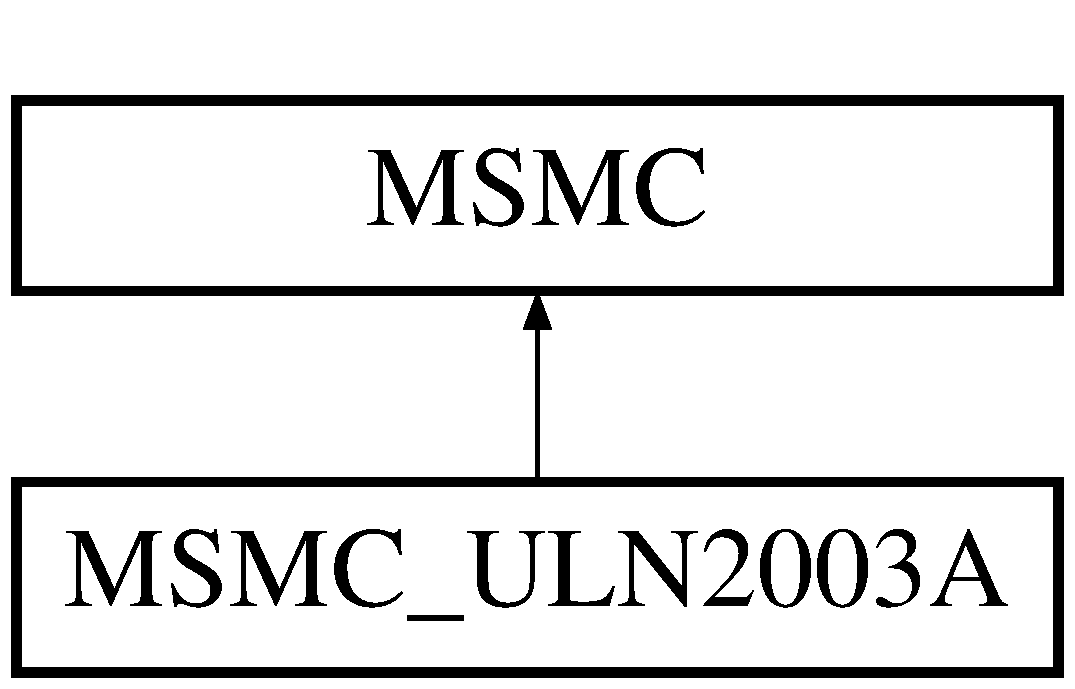
\includegraphics[height=2.000000cm]{class_m_s_m_c___u_l_n2003_a}
\end{center}
\end{figure}
\subsection*{Public Member Functions}
\begin{DoxyCompactItemize}
\item 
\hyperlink{class_m_s_m_c___u_l_n2003_a_a7b3b007290d0913572c5d42f23f6ed9a}{M\+S\+M\+C\+\_\+\+U\+L\+N2003\+A} ()
\begin{DoxyCompactList}\small\item\em Default constructor. \end{DoxyCompactList}\item 
\hyperlink{class_m_s_m_c___u_l_n2003_a_ae653d15c96f4e8ddfb4476cc77495ad1}{M\+S\+M\+C\+\_\+\+U\+L\+N2003\+A} (uint8\+\_\+t pin1, uint8\+\_\+t pin2, uint8\+\_\+t pin3, uint8\+\_\+t pin4)
\begin{DoxyCompactList}\small\item\em Constructor. \end{DoxyCompactList}\item 
void \hyperlink{class_m_s_m_c___u_l_n2003_a_a9657492f948a75472b311bc0b823899f}{forward} (uint32\+\_\+t st, uint32\+\_\+t sp)
\begin{DoxyCompactList}\small\item\em Configure the motor to move forward. \end{DoxyCompactList}\item 
void \hyperlink{class_m_s_m_c___u_l_n2003_a_ac46e6ec6345f95b534079bcf2920885e}{backward} (uint32\+\_\+t, uint32\+\_\+t)
\begin{DoxyCompactList}\small\item\em Configure the motor to move backward. \end{DoxyCompactList}\item 
void \hyperlink{class_m_s_m_c___u_l_n2003_a_a8a7f8b7e0048b3a03c87bd830d4a455f}{set\+Mode} (uint8\+\_\+t mod)
\begin{DoxyCompactList}\small\item\em Configure the operative mode of the controller. \end{DoxyCompactList}\item 
uint8\+\_\+t \hyperlink{class_m_s_m_c___u_l_n2003_a_a84cbd656e77e789af5cb34df147589a3}{get\+Mode} ()
\begin{DoxyCompactList}\small\item\em Return the operative mode of the controller. \end{DoxyCompactList}\item 
void \hyperlink{class_m_s_m_c___u_l_n2003_a_a19320fa4543dd8e76e338737690df235}{set\+Pins} (uint8\+\_\+t pin1, uint8\+\_\+t pin2, uint8\+\_\+t pin3, uint8\+\_\+t pin4)
\begin{DoxyCompactList}\small\item\em Change the pin mapping. \end{DoxyCompactList}\item 
void \hyperlink{class_m_s_m_c___u_l_n2003_a_ad8df164c90b2205fb65c796632889f82}{speed} (uint32\+\_\+t sp)
\begin{DoxyCompactList}\small\item\em Change the delay between each step. \end{DoxyCompactList}\item 
void \hyperlink{class_m_s_m_c___u_l_n2003_a_aba5e18f20f31fd4d6e71f50821dfeee5}{stop} ()
\begin{DoxyCompactList}\small\item\em Stop any motion. \end{DoxyCompactList}\item 
void \hyperlink{class_m_s_m_c___u_l_n2003_a_aa1d3444465d59ca6c87f05f565dde4a2}{pause} ()
\begin{DoxyCompactList}\small\item\em Pause the motion. \end{DoxyCompactList}\item 
void \hyperlink{class_m_s_m_c___u_l_n2003_a_a2af925737ce57e4b363b5cebb96e700b}{start} ()
\begin{DoxyCompactList}\small\item\em Restart the motion after the call of the function \hyperlink{class_m_s_m_c___u_l_n2003_a_aa1d3444465d59ca6c87f05f565dde4a2}{M\+S\+M\+C\+\_\+\+U\+L\+N2003\+A\+::pause()} \end{DoxyCompactList}\item 
int32\+\_\+t \hyperlink{class_m_s_m_c___u_l_n2003_a_a88c46f414c19fc81662abed58ce3fd92}{update} ()
\begin{DoxyCompactList}\small\item\em Perform the motion of the motor. \end{DoxyCompactList}\item 
void \hyperlink{class_m_s_m_c___u_l_n2003_a_aa6743162bdaba01ef1fc8a79f2519897}{print} ()
\begin{DoxyCompactList}\small\item\em Print in the serial channel the state of all inner variables. \end{DoxyCompactList}\end{DoxyCompactItemize}


\subsection{Detailed Description}
Multi Stepper Motor Control with U\+L\+N2003\+A. 

The class allows the contemporary control of multi stepper motors using the I\+Cs U\+L\+N2003\+A. After the motor setup, you can drive the motor forward and backward, specifying the number of steps and the delay in microseconds between two consecutive steps. The function update performs the effective motor motion, it must be call in the main loop and, if the delay is expired, the function moves the motor of one step. \begin{DoxyAuthor}{Author}
Francesco Giurlanda 
\end{DoxyAuthor}


\subsection{Constructor \& Destructor Documentation}
\hypertarget{class_m_s_m_c___u_l_n2003_a_a7b3b007290d0913572c5d42f23f6ed9a}{\index{M\+S\+M\+C\+\_\+\+U\+L\+N2003\+A@{M\+S\+M\+C\+\_\+\+U\+L\+N2003\+A}!M\+S\+M\+C\+\_\+\+U\+L\+N2003\+A@{M\+S\+M\+C\+\_\+\+U\+L\+N2003\+A}}
\index{M\+S\+M\+C\+\_\+\+U\+L\+N2003\+A@{M\+S\+M\+C\+\_\+\+U\+L\+N2003\+A}!M\+S\+M\+C\+\_\+\+U\+L\+N2003\+A@{M\+S\+M\+C\+\_\+\+U\+L\+N2003\+A}}
\subsubsection[{M\+S\+M\+C\+\_\+\+U\+L\+N2003\+A}]{\setlength{\rightskip}{0pt plus 5cm}M\+S\+M\+C\+\_\+\+U\+L\+N2003\+A\+::\+M\+S\+M\+C\+\_\+\+U\+L\+N2003\+A (
\begin{DoxyParamCaption}
{}
\end{DoxyParamCaption}
)}}\label{class_m_s_m_c___u_l_n2003_a_a7b3b007290d0913572c5d42f23f6ed9a}


Default constructor. 

\hypertarget{class_m_s_m_c___u_l_n2003_a_ae653d15c96f4e8ddfb4476cc77495ad1}{\index{M\+S\+M\+C\+\_\+\+U\+L\+N2003\+A@{M\+S\+M\+C\+\_\+\+U\+L\+N2003\+A}!M\+S\+M\+C\+\_\+\+U\+L\+N2003\+A@{M\+S\+M\+C\+\_\+\+U\+L\+N2003\+A}}
\index{M\+S\+M\+C\+\_\+\+U\+L\+N2003\+A@{M\+S\+M\+C\+\_\+\+U\+L\+N2003\+A}!M\+S\+M\+C\+\_\+\+U\+L\+N2003\+A@{M\+S\+M\+C\+\_\+\+U\+L\+N2003\+A}}
\subsubsection[{M\+S\+M\+C\+\_\+\+U\+L\+N2003\+A}]{\setlength{\rightskip}{0pt plus 5cm}M\+S\+M\+C\+\_\+\+U\+L\+N2003\+A\+::\+M\+S\+M\+C\+\_\+\+U\+L\+N2003\+A (
\begin{DoxyParamCaption}
\item[{uint8\+\_\+t}]{pin1, }
\item[{uint8\+\_\+t}]{pin2, }
\item[{uint8\+\_\+t}]{pin3, }
\item[{uint8\+\_\+t}]{pin4}
\end{DoxyParamCaption}
)}}\label{class_m_s_m_c___u_l_n2003_a_ae653d15c96f4e8ddfb4476cc77495ad1}


Constructor. 

Setup the pins where are attached the four coils of the unipolar motor. 
\begin{DoxyParams}{Parameters}
{\em pin1} & the pin connected to the coil 1a \\
\hline
{\em pin2} & the pin connected to the coil 2a \\
\hline
{\em pin3} & the pin connected to the coil 1b \\
\hline
{\em pin4} & the pin connected to the coil 2b \\
\hline
\end{DoxyParams}


\subsection{Member Function Documentation}
\hypertarget{class_m_s_m_c___u_l_n2003_a_ac46e6ec6345f95b534079bcf2920885e}{\index{M\+S\+M\+C\+\_\+\+U\+L\+N2003\+A@{M\+S\+M\+C\+\_\+\+U\+L\+N2003\+A}!backward@{backward}}
\index{backward@{backward}!M\+S\+M\+C\+\_\+\+U\+L\+N2003\+A@{M\+S\+M\+C\+\_\+\+U\+L\+N2003\+A}}
\subsubsection[{backward}]{\setlength{\rightskip}{0pt plus 5cm}void M\+S\+M\+C\+\_\+\+U\+L\+N2003\+A\+::backward (
\begin{DoxyParamCaption}
\item[{uint32\+\_\+t}]{st, }
\item[{uint32\+\_\+t}]{sp}
\end{DoxyParamCaption}
)\hspace{0.3cm}{\ttfamily [virtual]}}}\label{class_m_s_m_c___u_l_n2003_a_ac46e6ec6345f95b534079bcf2920885e}


Configure the motor to move backward. 

The function moves backward the motor of a number of steps with a specified delay betweet each step 
\begin{DoxyParams}{Parameters}
{\em st} & the number of steps \\
\hline
{\em sp} & the delay between the steps in microseconds \\
\hline
\end{DoxyParams}
\begin{DoxySeeAlso}{See also}
\hyperlink{class_m_s_m_c___u_l_n2003_a_a9657492f948a75472b311bc0b823899f}{forward(uint32\+\_\+t, uint32\+\_\+t)} 
\end{DoxySeeAlso}


Reimplemented from \hyperlink{class_m_s_m_c_a389bfe7f7d05083cb4e95d73128c1c87}{M\+S\+M\+C}.

\hypertarget{class_m_s_m_c___u_l_n2003_a_a9657492f948a75472b311bc0b823899f}{\index{M\+S\+M\+C\+\_\+\+U\+L\+N2003\+A@{M\+S\+M\+C\+\_\+\+U\+L\+N2003\+A}!forward@{forward}}
\index{forward@{forward}!M\+S\+M\+C\+\_\+\+U\+L\+N2003\+A@{M\+S\+M\+C\+\_\+\+U\+L\+N2003\+A}}
\subsubsection[{forward}]{\setlength{\rightskip}{0pt plus 5cm}void M\+S\+M\+C\+\_\+\+U\+L\+N2003\+A\+::forward (
\begin{DoxyParamCaption}
\item[{uint32\+\_\+t}]{st, }
\item[{uint32\+\_\+t}]{sp}
\end{DoxyParamCaption}
)\hspace{0.3cm}{\ttfamily [virtual]}}}\label{class_m_s_m_c___u_l_n2003_a_a9657492f948a75472b311bc0b823899f}


Configure the motor to move forward. 

The function moves forward the motor of a number of steps with a specified delay betweet each step 
\begin{DoxyParams}{Parameters}
{\em st} & the number of steps \\
\hline
{\em sp} & the delay between the steps in microseconds \\
\hline
\end{DoxyParams}
\begin{DoxySeeAlso}{See also}
\hyperlink{class_m_s_m_c___u_l_n2003_a_ac46e6ec6345f95b534079bcf2920885e}{backward(uint32\+\_\+t, uint32\+\_\+t)} 
\end{DoxySeeAlso}


Reimplemented from \hyperlink{class_m_s_m_c_a62615946a227d18ea3fc2f1329688d1f}{M\+S\+M\+C}.

\hypertarget{class_m_s_m_c___u_l_n2003_a_a84cbd656e77e789af5cb34df147589a3}{\index{M\+S\+M\+C\+\_\+\+U\+L\+N2003\+A@{M\+S\+M\+C\+\_\+\+U\+L\+N2003\+A}!get\+Mode@{get\+Mode}}
\index{get\+Mode@{get\+Mode}!M\+S\+M\+C\+\_\+\+U\+L\+N2003\+A@{M\+S\+M\+C\+\_\+\+U\+L\+N2003\+A}}
\subsubsection[{get\+Mode}]{\setlength{\rightskip}{0pt plus 5cm}uint8\+\_\+t M\+S\+M\+C\+\_\+\+U\+L\+N2003\+A\+::get\+Mode (
\begin{DoxyParamCaption}
{}
\end{DoxyParamCaption}
)\hspace{0.3cm}{\ttfamily [virtual]}}}\label{class_m_s_m_c___u_l_n2003_a_a84cbd656e77e789af5cb34df147589a3}


Return the operative mode of the controller. 

\begin{DoxyReturn}{Returns}
An int that identifies the operative mode\+: \hyperlink{_m_s_m_c___u_l_n2003_a_8h_a65ffcc85557e6fc00e865d67e20f720e}{F\+U\+L\+L\+\_\+\+S\+T\+E\+P} and \hyperlink{_m_s_m_c___u_l_n2003_a_8h_af078dda416ad0114e9c81a6c36c0801f}{H\+A\+L\+F\+\_\+\+S\+T\+E\+P} 
\end{DoxyReturn}


Reimplemented from \hyperlink{class_m_s_m_c_a5a1c4ee3498360946cc8e8d39436d0e3}{M\+S\+M\+C}.

\hypertarget{class_m_s_m_c___u_l_n2003_a_aa1d3444465d59ca6c87f05f565dde4a2}{\index{M\+S\+M\+C\+\_\+\+U\+L\+N2003\+A@{M\+S\+M\+C\+\_\+\+U\+L\+N2003\+A}!pause@{pause}}
\index{pause@{pause}!M\+S\+M\+C\+\_\+\+U\+L\+N2003\+A@{M\+S\+M\+C\+\_\+\+U\+L\+N2003\+A}}
\subsubsection[{pause}]{\setlength{\rightskip}{0pt plus 5cm}void M\+S\+M\+C\+\_\+\+U\+L\+N2003\+A\+::pause (
\begin{DoxyParamCaption}
{}
\end{DoxyParamCaption}
)\hspace{0.3cm}{\ttfamily [virtual]}}}\label{class_m_s_m_c___u_l_n2003_a_aa1d3444465d59ca6c87f05f565dde4a2}


Pause the motion. 

\begin{DoxySeeAlso}{See also}
\hyperlink{class_m_s_m_c___u_l_n2003_a_a2af925737ce57e4b363b5cebb96e700b}{M\+S\+M\+C\+\_\+\+U\+L\+N2003\+A\+::start()} 
\end{DoxySeeAlso}


Reimplemented from \hyperlink{class_m_s_m_c_a9c45f1547467b43209c7a271604e7c85}{M\+S\+M\+C}.

\hypertarget{class_m_s_m_c___u_l_n2003_a_aa6743162bdaba01ef1fc8a79f2519897}{\index{M\+S\+M\+C\+\_\+\+U\+L\+N2003\+A@{M\+S\+M\+C\+\_\+\+U\+L\+N2003\+A}!print@{print}}
\index{print@{print}!M\+S\+M\+C\+\_\+\+U\+L\+N2003\+A@{M\+S\+M\+C\+\_\+\+U\+L\+N2003\+A}}
\subsubsection[{print}]{\setlength{\rightskip}{0pt plus 5cm}void M\+S\+M\+C\+\_\+\+U\+L\+N2003\+A\+::print (
\begin{DoxyParamCaption}
{}
\end{DoxyParamCaption}
)}}\label{class_m_s_m_c___u_l_n2003_a_aa6743162bdaba01ef1fc8a79f2519897}


Print in the serial channel the state of all inner variables. 

\hypertarget{class_m_s_m_c___u_l_n2003_a_a8a7f8b7e0048b3a03c87bd830d4a455f}{\index{M\+S\+M\+C\+\_\+\+U\+L\+N2003\+A@{M\+S\+M\+C\+\_\+\+U\+L\+N2003\+A}!set\+Mode@{set\+Mode}}
\index{set\+Mode@{set\+Mode}!M\+S\+M\+C\+\_\+\+U\+L\+N2003\+A@{M\+S\+M\+C\+\_\+\+U\+L\+N2003\+A}}
\subsubsection[{set\+Mode}]{\setlength{\rightskip}{0pt plus 5cm}void M\+S\+M\+C\+\_\+\+U\+L\+N2003\+A\+::set\+Mode (
\begin{DoxyParamCaption}
\item[{uint8\+\_\+t}]{mod}
\end{DoxyParamCaption}
)\hspace{0.3cm}{\ttfamily [virtual]}}}\label{class_m_s_m_c___u_l_n2003_a_a8a7f8b7e0048b3a03c87bd830d4a455f}


Configure the operative mode of the controller. 


\begin{DoxyParams}{Parameters}
{\em mod} & The mode used by the controller, you can use the following macros\+:
\begin{DoxyItemize}
\item \hyperlink{_m_s_m_c___u_l_n2003_a_8h_a65ffcc85557e6fc00e865d67e20f720e}{F\+U\+L\+L\+\_\+\+S\+T\+E\+P}
\item \hyperlink{_m_s_m_c___u_l_n2003_a_8h_af078dda416ad0114e9c81a6c36c0801f}{H\+A\+L\+F\+\_\+\+S\+T\+E\+P} 
\end{DoxyItemize}\\
\hline
\end{DoxyParams}


Reimplemented from \hyperlink{class_m_s_m_c_a85bd4abf542aecdf24bb90b9ea2a47e9}{M\+S\+M\+C}.

\hypertarget{class_m_s_m_c___u_l_n2003_a_a19320fa4543dd8e76e338737690df235}{\index{M\+S\+M\+C\+\_\+\+U\+L\+N2003\+A@{M\+S\+M\+C\+\_\+\+U\+L\+N2003\+A}!set\+Pins@{set\+Pins}}
\index{set\+Pins@{set\+Pins}!M\+S\+M\+C\+\_\+\+U\+L\+N2003\+A@{M\+S\+M\+C\+\_\+\+U\+L\+N2003\+A}}
\subsubsection[{set\+Pins}]{\setlength{\rightskip}{0pt plus 5cm}void M\+S\+M\+C\+\_\+\+U\+L\+N2003\+A\+::set\+Pins (
\begin{DoxyParamCaption}
\item[{uint8\+\_\+t}]{pin1, }
\item[{uint8\+\_\+t}]{pin2, }
\item[{uint8\+\_\+t}]{pin3, }
\item[{uint8\+\_\+t}]{pin4}
\end{DoxyParamCaption}
)}}\label{class_m_s_m_c___u_l_n2003_a_a19320fa4543dd8e76e338737690df235}


Change the pin mapping. 


\begin{DoxyParams}{Parameters}
{\em pin1} & the pin connected to the coil 1a \\
\hline
{\em pin2} & the pin connected to the coil 2a \\
\hline
{\em pin3} & the pin connected to the coil 1b \\
\hline
{\em pin4} & the pin connected to the coil 2b \\
\hline
\end{DoxyParams}
\hypertarget{class_m_s_m_c___u_l_n2003_a_ad8df164c90b2205fb65c796632889f82}{\index{M\+S\+M\+C\+\_\+\+U\+L\+N2003\+A@{M\+S\+M\+C\+\_\+\+U\+L\+N2003\+A}!speed@{speed}}
\index{speed@{speed}!M\+S\+M\+C\+\_\+\+U\+L\+N2003\+A@{M\+S\+M\+C\+\_\+\+U\+L\+N2003\+A}}
\subsubsection[{speed}]{\setlength{\rightskip}{0pt plus 5cm}void M\+S\+M\+C\+\_\+\+U\+L\+N2003\+A\+::speed (
\begin{DoxyParamCaption}
\item[{uint32\+\_\+t}]{sp}
\end{DoxyParamCaption}
)\hspace{0.3cm}{\ttfamily [virtual]}}}\label{class_m_s_m_c___u_l_n2003_a_ad8df164c90b2205fb65c796632889f82}


Change the delay between each step. 

This function can be used to change the speed during an operation of forward or backward. 
\begin{DoxyParams}{Parameters}
{\em sp} & the delay in microseconds. \\
\hline
\end{DoxyParams}
\begin{DoxySeeAlso}{See also}
\hyperlink{class_m_s_m_c___u_l_n2003_a_a9657492f948a75472b311bc0b823899f}{forward(uint32\+\_\+t, uint32\+\_\+t)}, \hyperlink{class_m_s_m_c___u_l_n2003_a_ac46e6ec6345f95b534079bcf2920885e}{backward(uint32\+\_\+t, uint32\+\_\+t)} 
\end{DoxySeeAlso}


Reimplemented from \hyperlink{class_m_s_m_c_a065e48c8e8f3b513bf6694e8eb1b28d5}{M\+S\+M\+C}.

\hypertarget{class_m_s_m_c___u_l_n2003_a_a2af925737ce57e4b363b5cebb96e700b}{\index{M\+S\+M\+C\+\_\+\+U\+L\+N2003\+A@{M\+S\+M\+C\+\_\+\+U\+L\+N2003\+A}!start@{start}}
\index{start@{start}!M\+S\+M\+C\+\_\+\+U\+L\+N2003\+A@{M\+S\+M\+C\+\_\+\+U\+L\+N2003\+A}}
\subsubsection[{start}]{\setlength{\rightskip}{0pt plus 5cm}void M\+S\+M\+C\+\_\+\+U\+L\+N2003\+A\+::start (
\begin{DoxyParamCaption}
{}
\end{DoxyParamCaption}
)\hspace{0.3cm}{\ttfamily [virtual]}}}\label{class_m_s_m_c___u_l_n2003_a_a2af925737ce57e4b363b5cebb96e700b}


Restart the motion after the call of the function \hyperlink{class_m_s_m_c___u_l_n2003_a_aa1d3444465d59ca6c87f05f565dde4a2}{M\+S\+M\+C\+\_\+\+U\+L\+N2003\+A\+::pause()} 



Reimplemented from \hyperlink{class_m_s_m_c_a89abc0ac07d7010ba32d68840da1f822}{M\+S\+M\+C}.

\hypertarget{class_m_s_m_c___u_l_n2003_a_aba5e18f20f31fd4d6e71f50821dfeee5}{\index{M\+S\+M\+C\+\_\+\+U\+L\+N2003\+A@{M\+S\+M\+C\+\_\+\+U\+L\+N2003\+A}!stop@{stop}}
\index{stop@{stop}!M\+S\+M\+C\+\_\+\+U\+L\+N2003\+A@{M\+S\+M\+C\+\_\+\+U\+L\+N2003\+A}}
\subsubsection[{stop}]{\setlength{\rightskip}{0pt plus 5cm}void M\+S\+M\+C\+\_\+\+U\+L\+N2003\+A\+::stop (
\begin{DoxyParamCaption}
{}
\end{DoxyParamCaption}
)\hspace{0.3cm}{\ttfamily [virtual]}}}\label{class_m_s_m_c___u_l_n2003_a_aba5e18f20f31fd4d6e71f50821dfeee5}


Stop any motion. 



Reimplemented from \hyperlink{class_m_s_m_c_a0b44d0a659550ba754bf9212294ba6d5}{M\+S\+M\+C}.

\hypertarget{class_m_s_m_c___u_l_n2003_a_a88c46f414c19fc81662abed58ce3fd92}{\index{M\+S\+M\+C\+\_\+\+U\+L\+N2003\+A@{M\+S\+M\+C\+\_\+\+U\+L\+N2003\+A}!update@{update}}
\index{update@{update}!M\+S\+M\+C\+\_\+\+U\+L\+N2003\+A@{M\+S\+M\+C\+\_\+\+U\+L\+N2003\+A}}
\subsubsection[{update}]{\setlength{\rightskip}{0pt plus 5cm}int32\+\_\+t M\+S\+M\+C\+\_\+\+U\+L\+N2003\+A\+::update (
\begin{DoxyParamCaption}
{}
\end{DoxyParamCaption}
)\hspace{0.3cm}{\ttfamily [virtual]}}}\label{class_m_s_m_c___u_l_n2003_a_a88c46f414c19fc81662abed58ce3fd92}


Perform the motion of the motor. 

The function performs effectively the motor motion. It verifies that the specified delay from the last step is expired and than moves the motor of one step. The function must be call in the main loop with a frequency greater than 1/(delay$\ast$1000000). Greater is the frequency to call the function and higher is the precision of the the motion. \begin{DoxyReturn}{Returns}
the function number of steps made, up to the end of the motion. If the motion end the motor is idle and it can perform a new command. When the motor is idle the function returns -\/1. 
\end{DoxyReturn}


Reimplemented from \hyperlink{class_m_s_m_c_a44ca6bc355a269543606dd4eeb7ed06e}{M\+S\+M\+C}.



The documentation for this class was generated from the following files\+:\begin{DoxyCompactItemize}
\item 
\hyperlink{_m_s_m_c___u_l_n2003_a_8h}{M\+S\+M\+C\+\_\+\+U\+L\+N2003\+A.\+h}\item 
\hyperlink{_m_s_m_c___u_l_n2003_a_8cpp}{M\+S\+M\+C\+\_\+\+U\+L\+N2003\+A.\+cpp}\end{DoxyCompactItemize}

\hypertarget{class_plotter_servo}{\section{Plotter\+Servo Class Reference}
\label{class_plotter_servo}\index{Plotter\+Servo@{Plotter\+Servo}}
}


Class to control a plotter head.  




{\ttfamily \#include $<$Plotter\+Servo.\+h$>$}

Inheritance diagram for Plotter\+Servo\+:\begin{figure}[H]
\begin{center}
\leavevmode
\includegraphics[height=2.000000cm]{class_plotter_servo}
\end{center}
\end{figure}
\subsection*{Public Member Functions}
\begin{DoxyCompactItemize}
\item 
\hyperlink{class_plotter_servo_a3e1bb246a0c6b6df9f78b1a5a9343ef0}{Plotter\+Servo} (uint8\+\_\+t p, uint8\+\_\+t dv, uint8\+\_\+t uv)
\begin{DoxyCompactList}\small\item\em Constructor. \end{DoxyCompactList}\item 
void \hyperlink{class_plotter_servo_ad35c8f57eaeeffa768340a777c105aeb}{init} ()
\begin{DoxyCompactList}\small\item\em Initialize the object. It must be call into the \hyperlink{easy___c_n_c_8cpp_a4fc01d736fe50cf5b977f755b675f11d}{setup()}. \end{DoxyCompactList}\item 
boolean \hyperlink{class_plotter_servo_ab3d7dc74cd89c962a9cf27bdd210653f}{up} ()
\begin{DoxyCompactList}\small\item\em It moves the head up. \end{DoxyCompactList}\item 
boolean \hyperlink{class_plotter_servo_a06411670f5c5799ec84be0cffda3772b}{down} ()
\begin{DoxyCompactList}\small\item\em It moves the head down. \end{DoxyCompactList}\end{DoxyCompactItemize}
\subsection*{Private Attributes}
\begin{DoxyCompactItemize}
\item 
boolean \hyperlink{class_plotter_servo_a3309473d867ae37982f1ff0caba0c86b}{state}
\begin{DoxyCompactList}\small\item\em The state of the plotter head. \end{DoxyCompactList}\item 
uint8\+\_\+t \hyperlink{class_plotter_servo_a9c40d2afb9b5ae278deb8eab8b48a489}{pin}
\begin{DoxyCompactList}\small\item\em The pin where is attached the servo motor. \end{DoxyCompactList}\item 
Servo \hyperlink{class_plotter_servo_a9ecf1d8c79d1c73c3977198bb28b55a7}{servo\+\_\+pen}
\begin{DoxyCompactList}\small\item\em The object which control the servo motor. \end{DoxyCompactList}\item 
uint8\+\_\+t \hyperlink{class_plotter_servo_ad1150ec2c679af23d0a57cef4df7ff0a}{down\+\_\+val}
\begin{DoxyCompactList}\small\item\em The position of the servo for the plotter head down (deg) \end{DoxyCompactList}\item 
uint8\+\_\+t \hyperlink{class_plotter_servo_ac5a8cf60736715222a53a774c4e077f7}{up\+\_\+val}
\begin{DoxyCompactList}\small\item\em The position of the servo for the plotter head up (deg) \end{DoxyCompactList}\end{DoxyCompactItemize}


\subsection{Detailed Description}
Class to control a plotter head. 

The class allows to control an utensil with a per or a pencil or a marker pen, moved up and down by a servo motor. This utensil requires a P\+W\+M signal which controls the servo. \begin{DoxyAuthor}{Author}
Francesco Giurlanda 
\end{DoxyAuthor}


\subsection{Constructor \& Destructor Documentation}
\hypertarget{class_plotter_servo_a3e1bb246a0c6b6df9f78b1a5a9343ef0}{\index{Plotter\+Servo@{Plotter\+Servo}!Plotter\+Servo@{Plotter\+Servo}}
\index{Plotter\+Servo@{Plotter\+Servo}!Plotter\+Servo@{Plotter\+Servo}}
\subsubsection[{Plotter\+Servo}]{\setlength{\rightskip}{0pt plus 5cm}Plotter\+Servo\+::\+Plotter\+Servo (
\begin{DoxyParamCaption}
\item[{uint8\+\_\+t}]{p, }
\item[{uint8\+\_\+t}]{dv, }
\item[{uint8\+\_\+t}]{uv}
\end{DoxyParamCaption}
)}}\label{class_plotter_servo_a3e1bb246a0c6b6df9f78b1a5a9343ef0}


Constructor. 


\begin{DoxyParams}{Parameters}
{\em p} & The number of the pin where is attached the servo. \\
\hline
{\em dv} & The value for the plotter head down. \\
\hline
{\em uv} & The value for the plotter head up. \\
\hline
\end{DoxyParams}


\subsection{Member Function Documentation}
\hypertarget{class_plotter_servo_a06411670f5c5799ec84be0cffda3772b}{\index{Plotter\+Servo@{Plotter\+Servo}!down@{down}}
\index{down@{down}!Plotter\+Servo@{Plotter\+Servo}}
\subsubsection[{down}]{\setlength{\rightskip}{0pt plus 5cm}boolean Plotter\+Servo\+::down (
\begin{DoxyParamCaption}
{}
\end{DoxyParamCaption}
)}}\label{class_plotter_servo_a06411670f5c5799ec84be0cffda3772b}


It moves the head down. 

\hypertarget{class_plotter_servo_ad35c8f57eaeeffa768340a777c105aeb}{\index{Plotter\+Servo@{Plotter\+Servo}!init@{init}}
\index{init@{init}!Plotter\+Servo@{Plotter\+Servo}}
\subsubsection[{init}]{\setlength{\rightskip}{0pt plus 5cm}void Plotter\+Servo\+::init (
\begin{DoxyParamCaption}
{}
\end{DoxyParamCaption}
)}}\label{class_plotter_servo_ad35c8f57eaeeffa768340a777c105aeb}


Initialize the object. It must be call into the \hyperlink{easy___c_n_c_8cpp_a4fc01d736fe50cf5b977f755b675f11d}{setup()}. 

\hypertarget{class_plotter_servo_ab3d7dc74cd89c962a9cf27bdd210653f}{\index{Plotter\+Servo@{Plotter\+Servo}!up@{up}}
\index{up@{up}!Plotter\+Servo@{Plotter\+Servo}}
\subsubsection[{up}]{\setlength{\rightskip}{0pt plus 5cm}boolean Plotter\+Servo\+::up (
\begin{DoxyParamCaption}
{}
\end{DoxyParamCaption}
)}}\label{class_plotter_servo_ab3d7dc74cd89c962a9cf27bdd210653f}


It moves the head up. 



\subsection{Member Data Documentation}
\hypertarget{class_plotter_servo_ad1150ec2c679af23d0a57cef4df7ff0a}{\index{Plotter\+Servo@{Plotter\+Servo}!down\+\_\+val@{down\+\_\+val}}
\index{down\+\_\+val@{down\+\_\+val}!Plotter\+Servo@{Plotter\+Servo}}
\subsubsection[{down\+\_\+val}]{\setlength{\rightskip}{0pt plus 5cm}uint8\+\_\+t Plotter\+Servo\+::down\+\_\+val\hspace{0.3cm}{\ttfamily [private]}}}\label{class_plotter_servo_ad1150ec2c679af23d0a57cef4df7ff0a}


The position of the servo for the plotter head down (deg) 

\hypertarget{class_plotter_servo_a9c40d2afb9b5ae278deb8eab8b48a489}{\index{Plotter\+Servo@{Plotter\+Servo}!pin@{pin}}
\index{pin@{pin}!Plotter\+Servo@{Plotter\+Servo}}
\subsubsection[{pin}]{\setlength{\rightskip}{0pt plus 5cm}uint8\+\_\+t Plotter\+Servo\+::pin\hspace{0.3cm}{\ttfamily [private]}}}\label{class_plotter_servo_a9c40d2afb9b5ae278deb8eab8b48a489}


The pin where is attached the servo motor. 

\hypertarget{class_plotter_servo_a9ecf1d8c79d1c73c3977198bb28b55a7}{\index{Plotter\+Servo@{Plotter\+Servo}!servo\+\_\+pen@{servo\+\_\+pen}}
\index{servo\+\_\+pen@{servo\+\_\+pen}!Plotter\+Servo@{Plotter\+Servo}}
\subsubsection[{servo\+\_\+pen}]{\setlength{\rightskip}{0pt plus 5cm}Servo Plotter\+Servo\+::servo\+\_\+pen\hspace{0.3cm}{\ttfamily [private]}}}\label{class_plotter_servo_a9ecf1d8c79d1c73c3977198bb28b55a7}


The object which control the servo motor. 

\hypertarget{class_plotter_servo_a3309473d867ae37982f1ff0caba0c86b}{\index{Plotter\+Servo@{Plotter\+Servo}!state@{state}}
\index{state@{state}!Plotter\+Servo@{Plotter\+Servo}}
\subsubsection[{state}]{\setlength{\rightskip}{0pt plus 5cm}boolean Plotter\+Servo\+::state\hspace{0.3cm}{\ttfamily [private]}}}\label{class_plotter_servo_a3309473d867ae37982f1ff0caba0c86b}


The state of the plotter head. 

\begin{DoxySeeAlso}{See also}
\hyperlink{_plotter_servo_8h_a4193cd1c8c2e6ebd0e056fa2364a663f}{D\+O\+W\+N}, \hyperlink{_plotter_servo_8h_a1965eaca47dbf3f87acdafc2208f04eb}{U\+P} 
\end{DoxySeeAlso}
\hypertarget{class_plotter_servo_ac5a8cf60736715222a53a774c4e077f7}{\index{Plotter\+Servo@{Plotter\+Servo}!up\+\_\+val@{up\+\_\+val}}
\index{up\+\_\+val@{up\+\_\+val}!Plotter\+Servo@{Plotter\+Servo}}
\subsubsection[{up\+\_\+val}]{\setlength{\rightskip}{0pt plus 5cm}uint8\+\_\+t Plotter\+Servo\+::up\+\_\+val\hspace{0.3cm}{\ttfamily [private]}}}\label{class_plotter_servo_ac5a8cf60736715222a53a774c4e077f7}


The position of the servo for the plotter head up (deg) 



The documentation for this class was generated from the following files\+:\begin{DoxyCompactItemize}
\item 
utensils/\hyperlink{_plotter_servo_8h}{Plotter\+Servo.\+h}\item 
utensils/\hyperlink{_plotter_servo_8cpp}{Plotter\+Servo.\+cpp}\end{DoxyCompactItemize}

\hypertarget{class_position_x_y}{\section{Position\+X\+Y Class Reference}
\label{class_position_x_y}\index{Position\+X\+Y@{Position\+X\+Y}}
}


Class to manage cartesian position.  




{\ttfamily \#include $<$Position.\+h$>$}

\subsection*{Public Member Functions}
\begin{DoxyCompactItemize}
\item 
\hyperlink{class_position_x_y_a72c2bce8c3524d13a446e5f7bd00176b}{Position\+X\+Y} ()
\item 
\hyperlink{class_position_x_y_aa45af7bc859ed16de19470c46e476456}{Position\+X\+Y} (float px, float py)
\item 
\hyperlink{class_position_x_y_a3f71105e1c27ad675a24062942866fd4}{Position\+X\+Y} (const \hyperlink{class_position_x_y}{Position\+X\+Y} \&p)
\item 
float \hyperlink{class_position_x_y_a02c862d5e5a643a6d774b1876a30cc5e}{X} () const 
\item 
\hyperlink{class_position_x_y}{Position\+X\+Y} \& \hyperlink{class_position_x_y_aecca3ffac58837cd223add02a6145496}{X} (float px)
\item 
float \hyperlink{class_position_x_y_aa6bceb45b13566b4a312d5d7aad2ec77}{Y} () const 
\item 
\hyperlink{class_position_x_y}{Position\+X\+Y} \& \hyperlink{class_position_x_y_a7bb12f86083750580799fcf0535518e9}{Y} (float py)
\item 
float \hyperlink{class_position_x_y_a2e68cceafbc6d1a9d2956e64efbca1bf}{dist} (const \hyperlink{class_position_x_y}{Position\+X\+Y} \&p)
\item 
float \hyperlink{class_position_x_y_a781dce14528b62570fc4eed6318bab52}{dist\+X} (const \hyperlink{class_position_x_y}{Position\+X\+Y} \&p)
\item 
float \hyperlink{class_position_x_y_a099d374de2c2547108cbeba0cd6f89e2}{dist\+Y} (const \hyperlink{class_position_x_y}{Position\+X\+Y} \&p)
\item 
float \hyperlink{class_position_x_y_ab3a2559edfce2a9c6eb4ddc6ce456776}{angle} (const \hyperlink{class_position_x_y}{Position\+X\+Y} \&p)
\item 
\hyperlink{class_position_x_y}{Position\+X\+Y} \hyperlink{class_position_x_y_a8488dcd6f61a8019e6f3c6d147cf35c5}{operator+} (const \hyperlink{class_position_x_y}{Position\+X\+Y} \&p) const 
\item 
\hyperlink{class_position_x_y}{Position\+X\+Y} \& \hyperlink{class_position_x_y_a3c55c597bad99a80965b24781509e3fd}{operator+=} (const \hyperlink{class_position_x_y}{Position\+X\+Y} \&p)
\end{DoxyCompactItemize}


\subsection{Detailed Description}
Class to manage cartesian position. 

\subsection{Constructor \& Destructor Documentation}
\hypertarget{class_position_x_y_a72c2bce8c3524d13a446e5f7bd00176b}{\index{Position\+X\+Y@{Position\+X\+Y}!Position\+X\+Y@{Position\+X\+Y}}
\index{Position\+X\+Y@{Position\+X\+Y}!Position\+X\+Y@{Position\+X\+Y}}
\subsubsection[{Position\+X\+Y}]{\setlength{\rightskip}{0pt plus 5cm}Position\+X\+Y\+::\+Position\+X\+Y (
\begin{DoxyParamCaption}
{}
\end{DoxyParamCaption}
)}}\label{class_position_x_y_a72c2bce8c3524d13a446e5f7bd00176b}
\hypertarget{class_position_x_y_aa45af7bc859ed16de19470c46e476456}{\index{Position\+X\+Y@{Position\+X\+Y}!Position\+X\+Y@{Position\+X\+Y}}
\index{Position\+X\+Y@{Position\+X\+Y}!Position\+X\+Y@{Position\+X\+Y}}
\subsubsection[{Position\+X\+Y}]{\setlength{\rightskip}{0pt plus 5cm}Position\+X\+Y\+::\+Position\+X\+Y (
\begin{DoxyParamCaption}
\item[{float}]{px, }
\item[{float}]{py}
\end{DoxyParamCaption}
)}}\label{class_position_x_y_aa45af7bc859ed16de19470c46e476456}
\hypertarget{class_position_x_y_a3f71105e1c27ad675a24062942866fd4}{\index{Position\+X\+Y@{Position\+X\+Y}!Position\+X\+Y@{Position\+X\+Y}}
\index{Position\+X\+Y@{Position\+X\+Y}!Position\+X\+Y@{Position\+X\+Y}}
\subsubsection[{Position\+X\+Y}]{\setlength{\rightskip}{0pt plus 5cm}Position\+X\+Y\+::\+Position\+X\+Y (
\begin{DoxyParamCaption}
\item[{const {\bf Position\+X\+Y} \&}]{p}
\end{DoxyParamCaption}
)}}\label{class_position_x_y_a3f71105e1c27ad675a24062942866fd4}


\subsection{Member Function Documentation}
\hypertarget{class_position_x_y_ab3a2559edfce2a9c6eb4ddc6ce456776}{\index{Position\+X\+Y@{Position\+X\+Y}!angle@{angle}}
\index{angle@{angle}!Position\+X\+Y@{Position\+X\+Y}}
\subsubsection[{angle}]{\setlength{\rightskip}{0pt plus 5cm}float Position\+X\+Y\+::angle (
\begin{DoxyParamCaption}
\item[{const {\bf Position\+X\+Y} \&}]{p}
\end{DoxyParamCaption}
)\hspace{0.3cm}{\ttfamily [inline]}}}\label{class_position_x_y_ab3a2559edfce2a9c6eb4ddc6ce456776}
\hypertarget{class_position_x_y_a2e68cceafbc6d1a9d2956e64efbca1bf}{\index{Position\+X\+Y@{Position\+X\+Y}!dist@{dist}}
\index{dist@{dist}!Position\+X\+Y@{Position\+X\+Y}}
\subsubsection[{dist}]{\setlength{\rightskip}{0pt plus 5cm}float Position\+X\+Y\+::dist (
\begin{DoxyParamCaption}
\item[{const {\bf Position\+X\+Y} \&}]{p}
\end{DoxyParamCaption}
)\hspace{0.3cm}{\ttfamily [inline]}}}\label{class_position_x_y_a2e68cceafbc6d1a9d2956e64efbca1bf}
\hypertarget{class_position_x_y_a781dce14528b62570fc4eed6318bab52}{\index{Position\+X\+Y@{Position\+X\+Y}!dist\+X@{dist\+X}}
\index{dist\+X@{dist\+X}!Position\+X\+Y@{Position\+X\+Y}}
\subsubsection[{dist\+X}]{\setlength{\rightskip}{0pt plus 5cm}float Position\+X\+Y\+::dist\+X (
\begin{DoxyParamCaption}
\item[{const {\bf Position\+X\+Y} \&}]{p}
\end{DoxyParamCaption}
)}}\label{class_position_x_y_a781dce14528b62570fc4eed6318bab52}
\hypertarget{class_position_x_y_a099d374de2c2547108cbeba0cd6f89e2}{\index{Position\+X\+Y@{Position\+X\+Y}!dist\+Y@{dist\+Y}}
\index{dist\+Y@{dist\+Y}!Position\+X\+Y@{Position\+X\+Y}}
\subsubsection[{dist\+Y}]{\setlength{\rightskip}{0pt plus 5cm}float Position\+X\+Y\+::dist\+Y (
\begin{DoxyParamCaption}
\item[{const {\bf Position\+X\+Y} \&}]{p}
\end{DoxyParamCaption}
)}}\label{class_position_x_y_a099d374de2c2547108cbeba0cd6f89e2}
\hypertarget{class_position_x_y_a8488dcd6f61a8019e6f3c6d147cf35c5}{\index{Position\+X\+Y@{Position\+X\+Y}!operator+@{operator+}}
\index{operator+@{operator+}!Position\+X\+Y@{Position\+X\+Y}}
\subsubsection[{operator+}]{\setlength{\rightskip}{0pt plus 5cm}{\bf Position\+X\+Y} Position\+X\+Y\+::operator+ (
\begin{DoxyParamCaption}
\item[{const {\bf Position\+X\+Y} \&}]{p}
\end{DoxyParamCaption}
) const}}\label{class_position_x_y_a8488dcd6f61a8019e6f3c6d147cf35c5}
\hypertarget{class_position_x_y_a3c55c597bad99a80965b24781509e3fd}{\index{Position\+X\+Y@{Position\+X\+Y}!operator+=@{operator+=}}
\index{operator+=@{operator+=}!Position\+X\+Y@{Position\+X\+Y}}
\subsubsection[{operator+=}]{\setlength{\rightskip}{0pt plus 5cm}{\bf Position\+X\+Y} \& Position\+X\+Y\+::operator+= (
\begin{DoxyParamCaption}
\item[{const {\bf Position\+X\+Y} \&}]{p}
\end{DoxyParamCaption}
)}}\label{class_position_x_y_a3c55c597bad99a80965b24781509e3fd}
\hypertarget{class_position_x_y_a02c862d5e5a643a6d774b1876a30cc5e}{\index{Position\+X\+Y@{Position\+X\+Y}!X@{X}}
\index{X@{X}!Position\+X\+Y@{Position\+X\+Y}}
\subsubsection[{X}]{\setlength{\rightskip}{0pt plus 5cm}float Position\+X\+Y\+::\+X (
\begin{DoxyParamCaption}
{}
\end{DoxyParamCaption}
) const\hspace{0.3cm}{\ttfamily [inline]}}}\label{class_position_x_y_a02c862d5e5a643a6d774b1876a30cc5e}
\hypertarget{class_position_x_y_aecca3ffac58837cd223add02a6145496}{\index{Position\+X\+Y@{Position\+X\+Y}!X@{X}}
\index{X@{X}!Position\+X\+Y@{Position\+X\+Y}}
\subsubsection[{X}]{\setlength{\rightskip}{0pt plus 5cm}{\bf Position\+X\+Y} \& Position\+X\+Y\+::\+X (
\begin{DoxyParamCaption}
\item[{float}]{px}
\end{DoxyParamCaption}
)}}\label{class_position_x_y_aecca3ffac58837cd223add02a6145496}
\hypertarget{class_position_x_y_aa6bceb45b13566b4a312d5d7aad2ec77}{\index{Position\+X\+Y@{Position\+X\+Y}!Y@{Y}}
\index{Y@{Y}!Position\+X\+Y@{Position\+X\+Y}}
\subsubsection[{Y}]{\setlength{\rightskip}{0pt plus 5cm}float Position\+X\+Y\+::\+Y (
\begin{DoxyParamCaption}
{}
\end{DoxyParamCaption}
) const\hspace{0.3cm}{\ttfamily [inline]}}}\label{class_position_x_y_aa6bceb45b13566b4a312d5d7aad2ec77}
\hypertarget{class_position_x_y_a7bb12f86083750580799fcf0535518e9}{\index{Position\+X\+Y@{Position\+X\+Y}!Y@{Y}}
\index{Y@{Y}!Position\+X\+Y@{Position\+X\+Y}}
\subsubsection[{Y}]{\setlength{\rightskip}{0pt plus 5cm}{\bf Position\+X\+Y} \& Position\+X\+Y\+::\+Y (
\begin{DoxyParamCaption}
\item[{float}]{py}
\end{DoxyParamCaption}
)}}\label{class_position_x_y_a7bb12f86083750580799fcf0535518e9}


The documentation for this class was generated from the following files\+:\begin{DoxyCompactItemize}
\item 
\hyperlink{_position_8h}{Position.\+h}\item 
\hyperlink{_position_8cpp}{Position.\+cpp}\end{DoxyCompactItemize}

\input{class_position_x_y_z}
\input{class_timer}
\input{class_utensil}
\chapter{File Documentation}
\hypertarget{config_8h}{\section{config.\+h File Reference}
\label{config_8h}\index{config.\+h@{config.\+h}}
}


The configuration file.  


{\ttfamily \#include \char`\"{}pins\+\_\+arduino.\+h\char`\"{}}\\*
\subsection*{Macros}
\begin{DoxyCompactItemize}
\item 
\#define \hyperlink{config_8h_a58562c1eea53acf4d89ae2e8ed79e7ac}{S\+E\+R\+I\+A\+L\+\_\+\+B\+O\+U\+N\+D}~115200
\begin{DoxyCompactList}\small\item\em Define the speed of the serial comunication. \end{DoxyCompactList}\item 
\#define \hyperlink{config_8h_a11cc693021583511d43ba72c445120ea}{I\+N\+T\+E\+R\+R\+U\+P\+T\+\_\+\+S\+T\+O\+P\+\_\+\+M\+O\+T\+I\+O\+N}~1
\begin{DoxyCompactList}\small\item\em Define the number of the interrupt which is attached the stop button. \end{DoxyCompactList}\item 
\#define \hyperlink{config_8h_af30c7b107d77d612fa88c573d252c2c2}{R\+O\+U\+T\+E\+R\+\_\+\+M\+X\+\_\+\+S\+T\+E\+P\+S\+\_\+\+P\+E\+R\+\_\+\+R\+O\+U\+N\+D}~200
\begin{DoxyCompactList}\small\item\em Nunber of steps to make a round for the motor of the X-\/axis. \end{DoxyCompactList}\item 
\#define \hyperlink{config_8h_acea4b1619e299b0aff23f42c8ee5d84f}{R\+O\+U\+T\+E\+R\+\_\+\+M\+Y\+\_\+\+S\+T\+E\+P\+S\+\_\+\+P\+E\+R\+\_\+\+R\+O\+U\+N\+D}~200
\begin{DoxyCompactList}\small\item\em Nunber of steps to make a round for the motor of the Y-\/axis. \end{DoxyCompactList}\item 
\#define \hyperlink{config_8h_acc8d3a71b09ab28f1b65ee4b276355df}{R\+O\+U\+T\+E\+R\+\_\+\+M\+Z\+\_\+\+S\+T\+E\+P\+S\+\_\+\+P\+E\+R\+\_\+\+R\+O\+U\+N\+D}~200
\begin{DoxyCompactList}\small\item\em Nunber of steps to make a round for the motor of the Z-\/axis. \end{DoxyCompactList}\item 
\#define \hyperlink{config_8h_ad18fe160593d7a9ca8064b3f911c38cc}{R\+O\+U\+T\+E\+R\+\_\+\+M\+X\+\_\+\+S\+T\+E\+P\+S\+\_\+\+P\+E\+R\+\_\+\+M\+M}~\hyperlink{config_8h_af30c7b107d77d612fa88c573d252c2c2}{R\+O\+U\+T\+E\+R\+\_\+\+M\+X\+\_\+\+S\+T\+E\+P\+S\+\_\+\+P\+E\+R\+\_\+\+R\+O\+U\+N\+D}/1.\+256f
\begin{DoxyCompactList}\small\item\em Number of steps to forward of a mm. \end{DoxyCompactList}\item 
\#define \hyperlink{config_8h_afb07c4644cc35352a450b5b531fc7fa1}{R\+O\+U\+T\+E\+R\+\_\+\+M\+Y\+\_\+\+S\+T\+E\+P\+S\+\_\+\+P\+E\+R\+\_\+\+M\+M}~\hyperlink{config_8h_acea4b1619e299b0aff23f42c8ee5d84f}{R\+O\+U\+T\+E\+R\+\_\+\+M\+Y\+\_\+\+S\+T\+E\+P\+S\+\_\+\+P\+E\+R\+\_\+\+R\+O\+U\+N\+D}/1.\+25f
\begin{DoxyCompactList}\small\item\em Number of steps to forward of a mm. \end{DoxyCompactList}\item 
\#define \hyperlink{config_8h_a5ca3e0725b339b7fcb62e0cd353e1603}{R\+O\+U\+T\+E\+R\+\_\+\+M\+Z\+\_\+\+S\+T\+E\+P\+S\+\_\+\+P\+E\+R\+\_\+\+M\+M}~\hyperlink{config_8h_acc8d3a71b09ab28f1b65ee4b276355df}{R\+O\+U\+T\+E\+R\+\_\+\+M\+Z\+\_\+\+S\+T\+E\+P\+S\+\_\+\+P\+E\+R\+\_\+\+R\+O\+U\+N\+D}/1.\+256f
\begin{DoxyCompactList}\small\item\em Number of steps to forward of a mm. \end{DoxyCompactList}\item 
\#define \hyperlink{config_8h_a67b3c67678c03bf1911716033c3ea33d}{R\+O\+U\+T\+E\+R\+\_\+\+M\+X\+\_\+\+O\+R\+I\+E\+N\+T\+A\+T\+I\+O\+N}~-\/1
\item 
\#define \hyperlink{config_8h_a28b6bbdef359a6ba4d79d34fe398ce65}{R\+O\+U\+T\+E\+R\+\_\+\+M\+Y\+\_\+\+O\+R\+I\+E\+N\+T\+A\+T\+I\+O\+N}~1
\item 
\#define \hyperlink{config_8h_a7e901586d0efb8802e56099c23b52124}{R\+O\+U\+T\+E\+R\+\_\+\+M\+Z\+\_\+\+O\+R\+I\+E\+N\+T\+A\+T\+I\+O\+N}~1
\item 
\#define \hyperlink{config_8h_aeb39dfe1cecb49617c2de68f2b7863ad}{R\+O\+U\+T\+E\+R\+\_\+\+M\+X\+\_\+\+S\+P\+E\+E\+D}~2400.\+0
\begin{DoxyCompactList}\small\item\em The maximum speed used to control the motor of X-\/axis (steps/s). \end{DoxyCompactList}\item 
\#define \hyperlink{config_8h_a561a2d9e0685a3f1ef859e8fe82c44ee}{R\+O\+U\+T\+E\+R\+\_\+\+M\+Y\+\_\+\+S\+P\+E\+E\+D}~2400.\+0
\begin{DoxyCompactList}\small\item\em The maximum speed used to control the motor of Y-\/axis (steps/s). \end{DoxyCompactList}\item 
\#define \hyperlink{config_8h_a8437dbcba761d0ae49161e7e16dbe94d}{R\+O\+U\+T\+E\+R\+\_\+\+M\+Z\+\_\+\+S\+P\+E\+E\+D}~2400.\+0
\begin{DoxyCompactList}\small\item\em The maximum speed used to control the motor of Z-\/axis (steps/s). \end{DoxyCompactList}\item 
\#define \hyperlink{config_8h_a569578859eb9df4de5175738b3a1ade1}{R\+O\+U\+T\+E\+R\+\_\+\+D\+O\+W\+N\+\_\+\+L\+I\+M\+I\+T\+\_\+\+S\+W\+I\+T\+C\+H\+\_\+\+X\+\_\+\+I\+N\+T\+E\+R\+R\+U\+P\+T}~1
\begin{DoxyCompactList}\small\item\em The number of the interrupt which is connected to the down limit switch of the X-\/axis. It is different by the pin number. More details \href{http://arduino.cc/en/Reference/AttachInterrupt}{\tt here}. The value -\/1 means that it is disconnected. \end{DoxyCompactList}\item 
\#define \hyperlink{config_8h_aa8a396530fa7d038d900e79c9906f1f3}{R\+O\+U\+T\+E\+R\+\_\+\+D\+O\+W\+N\+\_\+\+L\+I\+M\+I\+T\+\_\+\+S\+W\+I\+T\+C\+H\+\_\+\+Y\+\_\+\+I\+N\+T\+E\+R\+R\+U\+P\+T}~0
\begin{DoxyCompactList}\small\item\em The number of the interrupt which is connected to the down limit switch of the Y-\/axis. It is different by the pin number. More details \href{http://arduino.cc/en/Reference/AttachInterrupt}{\tt here}. The value -\/1 means that it is disconnected. \end{DoxyCompactList}\item 
\#define \hyperlink{config_8h_a8f25718b319cc5f5ae8c2cd6a0bd47b1}{R\+O\+U\+T\+E\+R\+\_\+\+D\+O\+W\+N\+\_\+\+L\+I\+M\+I\+T\+\_\+\+S\+W\+I\+T\+C\+H\+\_\+\+Z\+\_\+\+I\+N\+T\+E\+R\+R\+U\+P\+T}~-\/1
\item 
\#define \hyperlink{config_8h_a6837a9e9e13c670013e9d9be10ce8534}{R\+O\+U\+T\+E\+R\+\_\+\+U\+P\+\_\+\+L\+I\+M\+I\+T\+\_\+\+S\+W\+I\+T\+C\+H\+\_\+\+X\+\_\+\+I\+N\+T\+E\+R\+R\+U\+P\+T}~-\/1
\begin{DoxyCompactList}\small\item\em T\+The number of the interrupt which is connected to the up limit switch of the X-\/axis. It is different by the pin number. More details \href{http://arduino.cc/en/Reference/AttachInterrupt}{\tt here}. The value -\/1 means that it is disconnected. \end{DoxyCompactList}\item 
\#define \hyperlink{config_8h_a361d56e382a8888abf494198209f4ceb}{R\+O\+U\+T\+E\+R\+\_\+\+U\+P\+\_\+\+L\+I\+M\+I\+T\+\_\+\+S\+W\+I\+T\+C\+H\+\_\+\+Y\+\_\+\+I\+N\+T\+E\+R\+R\+U\+P\+T}~-\/1
\begin{DoxyCompactList}\small\item\em T\+The number of the interrupt which is connected to the up limit switch of the Y-\/axis. It is different by the pin number. More details \href{http://arduino.cc/en/Reference/AttachInterrupt}{\tt here}. The value -\/1 means that it is disconnected. \end{DoxyCompactList}\item 
\#define \hyperlink{config_8h_a3f2c7573e3dc8e95df6b528e98a81626}{R\+O\+U\+T\+E\+R\+\_\+\+U\+P\+\_\+\+L\+I\+M\+I\+T\+\_\+\+S\+W\+I\+T\+C\+H\+\_\+\+Z\+\_\+\+I\+N\+T\+E\+R\+R\+U\+P\+T}~-\/1
\begin{DoxyCompactList}\small\item\em T\+The number of the interrupt which is connected to the up limit switch of the Z-\/axis. It is different by the pin number. More details \href{http://arduino.cc/en/Reference/AttachInterrupt}{\tt here}. The value -\/1 means that it is disconnected. \end{DoxyCompactList}\item 
\#define \hyperlink{config_8h_aa2ba8973ad8e317ff2808a08cd03109d}{R\+O\+U\+T\+E\+R\+\_\+\+M\+X\+\_\+\+C\+O\+N\+T\+R\+O\+L\+L\+E\+R\+\_\+\+A4988}
\item 
\#define \hyperlink{config_8h_a2772e27b33c24fca3e756e98e4da0528}{R\+O\+U\+T\+E\+\_\+\+M\+X\+\_\+\+S\+T\+E\+P\+\_\+\+C\+O\+N\+T\+R\+O\+L\+\_\+\+P\+I\+N}~A0
\begin{DoxyCompactList}\small\item\em Pin connected to the step control pin of the A4988. \end{DoxyCompactList}\item 
\#define \hyperlink{config_8h_a458d8330a8ea0e864a5f14641beaff3b}{R\+O\+U\+T\+E\+\_\+\+M\+X\+\_\+\+D\+I\+R\+E\+C\+T\+I\+O\+N\+\_\+\+C\+O\+N\+T\+R\+O\+L\+\_\+\+P\+I\+N}~A1
\begin{DoxyCompactList}\small\item\em Pin connected to the direction control pin of the A4988. \end{DoxyCompactList}\item 
\#define \hyperlink{config_8h_aa440cb6779843ab1068ff26919b75db4}{R\+O\+U\+T\+E\+\_\+\+M\+X\+\_\+\+E\+N\+A\+B\+L\+E\+\_\+\+C\+O\+N\+T\+R\+O\+L\+\_\+\+P\+I\+N}~38
\begin{DoxyCompactList}\small\item\em Pin connected to the enable pin of the A4988. \end{DoxyCompactList}\item 
\#define \hyperlink{config_8h_a40d4a3ddd9f57ccbf4a39547f75aaffd}{R\+O\+U\+T\+E\+\_\+\+M\+X\+\_\+\+M\+O\+D\+E}~\hyperlink{_m_s_m_c___a4988_8h_a5bf980ea8dd6df6a0271f6d30d66931b}{Q\+U\+A\+R\+T\+E\+R\+\_\+\+S\+T\+E\+P}
\begin{DoxyCompactList}\small\item\em The microstep mode of the driver of the motor X. \end{DoxyCompactList}\item 
\#define \hyperlink{config_8h_ab43f3d9753eb04addb3ecf892d43e9b3}{R\+O\+U\+T\+E\+R\+\_\+\+M\+Y\+\_\+\+C\+O\+N\+T\+R\+O\+L\+L\+E\+R\+\_\+\+A4988}
\item 
\#define \hyperlink{config_8h_ab22bf58b0951dd8f3ae5d94bda82d87e}{R\+O\+U\+T\+E\+\_\+\+M\+Y\+\_\+\+S\+T\+E\+P\+\_\+\+C\+O\+N\+T\+R\+O\+L\+\_\+\+P\+I\+N}~46
\begin{DoxyCompactList}\small\item\em Pin connected to the step control pin of the A4988. \end{DoxyCompactList}\item 
\#define \hyperlink{config_8h_a865681c0605dcc31e4c0262995aaef20}{R\+O\+U\+T\+E\+\_\+\+M\+Y\+\_\+\+D\+I\+R\+E\+C\+T\+I\+O\+N\+\_\+\+C\+O\+N\+T\+R\+O\+L\+\_\+\+P\+I\+N}~48
\begin{DoxyCompactList}\small\item\em Pin connected to the direction control pin of the A4988. \end{DoxyCompactList}\item 
\#define \hyperlink{config_8h_a3e30826a0cbcd6ac91bae8b83651bc78}{R\+O\+U\+T\+E\+\_\+\+M\+Y\+\_\+\+E\+N\+A\+B\+L\+E\+\_\+\+C\+O\+N\+T\+R\+O\+L\+\_\+\+P\+I\+N}~A8
\begin{DoxyCompactList}\small\item\em Pin connected to the enable pin of the A4988. \end{DoxyCompactList}\item 
\#define \hyperlink{config_8h_a2d8287db2902bf9aa81078f7131854f1}{R\+O\+U\+T\+E\+\_\+\+M\+Y\+\_\+\+M\+O\+D\+E}~\hyperlink{_m_s_m_c___a4988_8h_a5bf980ea8dd6df6a0271f6d30d66931b}{Q\+U\+A\+R\+T\+E\+R\+\_\+\+S\+T\+E\+P}
\begin{DoxyCompactList}\small\item\em The microstep mode of the driver of the motor Y. \end{DoxyCompactList}\item 
\#define \hyperlink{config_8h_a09fa750e355606467364b15acc58a814}{R\+O\+U\+T\+E\+R\+\_\+\+M\+Z\+\_\+\+C\+O\+N\+T\+R\+O\+L\+L\+E\+R\+\_\+\+A4988}
\item 
\#define \hyperlink{config_8h_a19711e5668de2b87dad0e16a5e863743}{R\+O\+U\+T\+E\+\_\+\+M\+Z\+\_\+\+S\+T\+E\+P\+\_\+\+C\+O\+N\+T\+R\+O\+L\+\_\+\+P\+I\+N}~A6
\begin{DoxyCompactList}\small\item\em Pin connected to the step control pin of the A4988. \end{DoxyCompactList}\item 
\#define \hyperlink{config_8h_a5b6402fd081aead9dc14384deb017036}{R\+O\+U\+T\+E\+\_\+\+M\+Z\+\_\+\+D\+I\+R\+E\+C\+T\+I\+O\+N\+\_\+\+C\+O\+N\+T\+R\+O\+L\+\_\+\+P\+I\+N}~A7
\begin{DoxyCompactList}\small\item\em Pin connected to the direction control pin of the A4988. \end{DoxyCompactList}\item 
\#define \hyperlink{config_8h_a5cbe1ee81d34630a1e50fa9c42436082}{R\+O\+U\+T\+E\+\_\+\+M\+Z\+\_\+\+E\+N\+A\+B\+L\+E\+\_\+\+C\+O\+N\+T\+R\+O\+L\+\_\+\+P\+I\+N}~A2
\begin{DoxyCompactList}\small\item\em Pin connected to the enable pin of the A4988. \end{DoxyCompactList}\item 
\#define \hyperlink{config_8h_a54facf4e6f0019a0b22b92d523fe2cdc}{R\+O\+U\+T\+E\+\_\+\+M\+Z\+\_\+\+M\+O\+D\+E}~\hyperlink{_m_s_m_c___a4988_8h_a5bf980ea8dd6df6a0271f6d30d66931b}{Q\+U\+A\+R\+T\+E\+R\+\_\+\+S\+T\+E\+P}
\begin{DoxyCompactList}\small\item\em The microstep mode of the driver of the motor Z. \end{DoxyCompactList}\item 
\#define \hyperlink{config_8h_a1ed2a15e6b761d36ac89dfc727d4ae82}{\+\_\+\+M\+I\+L\+L\+I\+N\+G\+\_\+\+M\+A\+C\+H\+I\+N\+E}
\begin{DoxyCompactList}\small\item\em Uncomment to active the milling machine support. \end{DoxyCompactList}\item 
\#define \hyperlink{config_8h_a32622311332cb8ba6ba14a69ce19f70e}{\+\_\+\+M\+I\+L\+L\+I\+N\+G\+\_\+\+M\+A\+C\+H\+I\+N\+E\+\_\+\+E\+N\+A\+B\+L\+E\+\_\+\+P\+I\+N}~10
\begin{DoxyCompactList}\small\item\em The pin number connected to the enable circuit of the milling machine. \end{DoxyCompactList}\item 
\#define \hyperlink{config_8h_a11bacbdfb698dadd088b8d0ba265ace4}{\+\_\+\+M\+I\+L\+L\+I\+N\+G\+\_\+\+M\+A\+C\+H\+I\+N\+E\+\_\+\+S\+P\+E\+E\+D\+\_\+\+P\+I\+N}~11
\begin{DoxyCompactList}\small\item\em The pin number connected to the speed control circuit of the milling machine. \end{DoxyCompactList}\end{DoxyCompactItemize}


\subsection{Detailed Description}
The configuration file. 

In this file there are all the configurable parameters. \begin{DoxyAuthor}{Author}
Francesco Giurlanda 
\end{DoxyAuthor}
\begin{DoxyVersion}{Version}
0.\+0.\+1 
\end{DoxyVersion}
\begin{DoxyDate}{Date}
2014 
\end{DoxyDate}
\begin{DoxyWarning}{Warning}
If you change Arduino board some parameters could change too. 
\end{DoxyWarning}
\begin{DoxyCopyright}{Copyright}
This work is licensed under the Creative Commons Attribution-\/\+Share\+Alike 4.\+0 International License. To view a copy of this license, visit \href{http://creativecommons.org/licenses/by-sa/4.0/}{\tt http\+://creativecommons.\+org/licenses/by-\/sa/4.\+0/}. 
\end{DoxyCopyright}


\subsection{Macro Definition Documentation}
\hypertarget{config_8h_a1ed2a15e6b761d36ac89dfc727d4ae82}{\index{config.\+h@{config.\+h}!\+\_\+\+M\+I\+L\+L\+I\+N\+G\+\_\+\+M\+A\+C\+H\+I\+N\+E@{\+\_\+\+M\+I\+L\+L\+I\+N\+G\+\_\+\+M\+A\+C\+H\+I\+N\+E}}
\index{\+\_\+\+M\+I\+L\+L\+I\+N\+G\+\_\+\+M\+A\+C\+H\+I\+N\+E@{\+\_\+\+M\+I\+L\+L\+I\+N\+G\+\_\+\+M\+A\+C\+H\+I\+N\+E}!config.\+h@{config.\+h}}
\subsubsection[{\+\_\+\+M\+I\+L\+L\+I\+N\+G\+\_\+\+M\+A\+C\+H\+I\+N\+E}]{\setlength{\rightskip}{0pt plus 5cm}\#define \+\_\+\+M\+I\+L\+L\+I\+N\+G\+\_\+\+M\+A\+C\+H\+I\+N\+E}}\label{config_8h_a1ed2a15e6b761d36ac89dfc727d4ae82}


Uncomment to active the milling machine support. 

\hypertarget{config_8h_a32622311332cb8ba6ba14a69ce19f70e}{\index{config.\+h@{config.\+h}!\+\_\+\+M\+I\+L\+L\+I\+N\+G\+\_\+\+M\+A\+C\+H\+I\+N\+E\+\_\+\+E\+N\+A\+B\+L\+E\+\_\+\+P\+I\+N@{\+\_\+\+M\+I\+L\+L\+I\+N\+G\+\_\+\+M\+A\+C\+H\+I\+N\+E\+\_\+\+E\+N\+A\+B\+L\+E\+\_\+\+P\+I\+N}}
\index{\+\_\+\+M\+I\+L\+L\+I\+N\+G\+\_\+\+M\+A\+C\+H\+I\+N\+E\+\_\+\+E\+N\+A\+B\+L\+E\+\_\+\+P\+I\+N@{\+\_\+\+M\+I\+L\+L\+I\+N\+G\+\_\+\+M\+A\+C\+H\+I\+N\+E\+\_\+\+E\+N\+A\+B\+L\+E\+\_\+\+P\+I\+N}!config.\+h@{config.\+h}}
\subsubsection[{\+\_\+\+M\+I\+L\+L\+I\+N\+G\+\_\+\+M\+A\+C\+H\+I\+N\+E\+\_\+\+E\+N\+A\+B\+L\+E\+\_\+\+P\+I\+N}]{\setlength{\rightskip}{0pt plus 5cm}\#define \+\_\+\+M\+I\+L\+L\+I\+N\+G\+\_\+\+M\+A\+C\+H\+I\+N\+E\+\_\+\+E\+N\+A\+B\+L\+E\+\_\+\+P\+I\+N~10}}\label{config_8h_a32622311332cb8ba6ba14a69ce19f70e}


The pin number connected to the enable circuit of the milling machine. 

\hypertarget{config_8h_a11bacbdfb698dadd088b8d0ba265ace4}{\index{config.\+h@{config.\+h}!\+\_\+\+M\+I\+L\+L\+I\+N\+G\+\_\+\+M\+A\+C\+H\+I\+N\+E\+\_\+\+S\+P\+E\+E\+D\+\_\+\+P\+I\+N@{\+\_\+\+M\+I\+L\+L\+I\+N\+G\+\_\+\+M\+A\+C\+H\+I\+N\+E\+\_\+\+S\+P\+E\+E\+D\+\_\+\+P\+I\+N}}
\index{\+\_\+\+M\+I\+L\+L\+I\+N\+G\+\_\+\+M\+A\+C\+H\+I\+N\+E\+\_\+\+S\+P\+E\+E\+D\+\_\+\+P\+I\+N@{\+\_\+\+M\+I\+L\+L\+I\+N\+G\+\_\+\+M\+A\+C\+H\+I\+N\+E\+\_\+\+S\+P\+E\+E\+D\+\_\+\+P\+I\+N}!config.\+h@{config.\+h}}
\subsubsection[{\+\_\+\+M\+I\+L\+L\+I\+N\+G\+\_\+\+M\+A\+C\+H\+I\+N\+E\+\_\+\+S\+P\+E\+E\+D\+\_\+\+P\+I\+N}]{\setlength{\rightskip}{0pt plus 5cm}\#define \+\_\+\+M\+I\+L\+L\+I\+N\+G\+\_\+\+M\+A\+C\+H\+I\+N\+E\+\_\+\+S\+P\+E\+E\+D\+\_\+\+P\+I\+N~11}}\label{config_8h_a11bacbdfb698dadd088b8d0ba265ace4}


The pin number connected to the speed control circuit of the milling machine. 

\hypertarget{config_8h_a11cc693021583511d43ba72c445120ea}{\index{config.\+h@{config.\+h}!I\+N\+T\+E\+R\+R\+U\+P\+T\+\_\+\+S\+T\+O\+P\+\_\+\+M\+O\+T\+I\+O\+N@{I\+N\+T\+E\+R\+R\+U\+P\+T\+\_\+\+S\+T\+O\+P\+\_\+\+M\+O\+T\+I\+O\+N}}
\index{I\+N\+T\+E\+R\+R\+U\+P\+T\+\_\+\+S\+T\+O\+P\+\_\+\+M\+O\+T\+I\+O\+N@{I\+N\+T\+E\+R\+R\+U\+P\+T\+\_\+\+S\+T\+O\+P\+\_\+\+M\+O\+T\+I\+O\+N}!config.\+h@{config.\+h}}
\subsubsection[{I\+N\+T\+E\+R\+R\+U\+P\+T\+\_\+\+S\+T\+O\+P\+\_\+\+M\+O\+T\+I\+O\+N}]{\setlength{\rightskip}{0pt plus 5cm}\#define I\+N\+T\+E\+R\+R\+U\+P\+T\+\_\+\+S\+T\+O\+P\+\_\+\+M\+O\+T\+I\+O\+N~1}}\label{config_8h_a11cc693021583511d43ba72c445120ea}


Define the number of the interrupt which is attached the stop button. 

This value is different from the pin number at which the interrupt refers. The pin depends on the arduino board version. See \href{http://arduino.cc/en/Main/Products}{\tt http\+://arduino.\+cc/en/\+Main/\+Products} \hypertarget{config_8h_a458d8330a8ea0e864a5f14641beaff3b}{\index{config.\+h@{config.\+h}!R\+O\+U\+T\+E\+\_\+\+M\+X\+\_\+\+D\+I\+R\+E\+C\+T\+I\+O\+N\+\_\+\+C\+O\+N\+T\+R\+O\+L\+\_\+\+P\+I\+N@{R\+O\+U\+T\+E\+\_\+\+M\+X\+\_\+\+D\+I\+R\+E\+C\+T\+I\+O\+N\+\_\+\+C\+O\+N\+T\+R\+O\+L\+\_\+\+P\+I\+N}}
\index{R\+O\+U\+T\+E\+\_\+\+M\+X\+\_\+\+D\+I\+R\+E\+C\+T\+I\+O\+N\+\_\+\+C\+O\+N\+T\+R\+O\+L\+\_\+\+P\+I\+N@{R\+O\+U\+T\+E\+\_\+\+M\+X\+\_\+\+D\+I\+R\+E\+C\+T\+I\+O\+N\+\_\+\+C\+O\+N\+T\+R\+O\+L\+\_\+\+P\+I\+N}!config.\+h@{config.\+h}}
\subsubsection[{R\+O\+U\+T\+E\+\_\+\+M\+X\+\_\+\+D\+I\+R\+E\+C\+T\+I\+O\+N\+\_\+\+C\+O\+N\+T\+R\+O\+L\+\_\+\+P\+I\+N}]{\setlength{\rightskip}{0pt plus 5cm}\#define R\+O\+U\+T\+E\+\_\+\+M\+X\+\_\+\+D\+I\+R\+E\+C\+T\+I\+O\+N\+\_\+\+C\+O\+N\+T\+R\+O\+L\+\_\+\+P\+I\+N~A1}}\label{config_8h_a458d8330a8ea0e864a5f14641beaff3b}


Pin connected to the direction control pin of the A4988. 

\hypertarget{config_8h_aa440cb6779843ab1068ff26919b75db4}{\index{config.\+h@{config.\+h}!R\+O\+U\+T\+E\+\_\+\+M\+X\+\_\+\+E\+N\+A\+B\+L\+E\+\_\+\+C\+O\+N\+T\+R\+O\+L\+\_\+\+P\+I\+N@{R\+O\+U\+T\+E\+\_\+\+M\+X\+\_\+\+E\+N\+A\+B\+L\+E\+\_\+\+C\+O\+N\+T\+R\+O\+L\+\_\+\+P\+I\+N}}
\index{R\+O\+U\+T\+E\+\_\+\+M\+X\+\_\+\+E\+N\+A\+B\+L\+E\+\_\+\+C\+O\+N\+T\+R\+O\+L\+\_\+\+P\+I\+N@{R\+O\+U\+T\+E\+\_\+\+M\+X\+\_\+\+E\+N\+A\+B\+L\+E\+\_\+\+C\+O\+N\+T\+R\+O\+L\+\_\+\+P\+I\+N}!config.\+h@{config.\+h}}
\subsubsection[{R\+O\+U\+T\+E\+\_\+\+M\+X\+\_\+\+E\+N\+A\+B\+L\+E\+\_\+\+C\+O\+N\+T\+R\+O\+L\+\_\+\+P\+I\+N}]{\setlength{\rightskip}{0pt plus 5cm}\#define R\+O\+U\+T\+E\+\_\+\+M\+X\+\_\+\+E\+N\+A\+B\+L\+E\+\_\+\+C\+O\+N\+T\+R\+O\+L\+\_\+\+P\+I\+N~38}}\label{config_8h_aa440cb6779843ab1068ff26919b75db4}


Pin connected to the enable pin of the A4988. 

\hypertarget{config_8h_a40d4a3ddd9f57ccbf4a39547f75aaffd}{\index{config.\+h@{config.\+h}!R\+O\+U\+T\+E\+\_\+\+M\+X\+\_\+\+M\+O\+D\+E@{R\+O\+U\+T\+E\+\_\+\+M\+X\+\_\+\+M\+O\+D\+E}}
\index{R\+O\+U\+T\+E\+\_\+\+M\+X\+\_\+\+M\+O\+D\+E@{R\+O\+U\+T\+E\+\_\+\+M\+X\+\_\+\+M\+O\+D\+E}!config.\+h@{config.\+h}}
\subsubsection[{R\+O\+U\+T\+E\+\_\+\+M\+X\+\_\+\+M\+O\+D\+E}]{\setlength{\rightskip}{0pt plus 5cm}\#define R\+O\+U\+T\+E\+\_\+\+M\+X\+\_\+\+M\+O\+D\+E~{\bf Q\+U\+A\+R\+T\+E\+R\+\_\+\+S\+T\+E\+P}}}\label{config_8h_a40d4a3ddd9f57ccbf4a39547f75aaffd}


The microstep mode of the driver of the motor X. 

\hypertarget{config_8h_a2772e27b33c24fca3e756e98e4da0528}{\index{config.\+h@{config.\+h}!R\+O\+U\+T\+E\+\_\+\+M\+X\+\_\+\+S\+T\+E\+P\+\_\+\+C\+O\+N\+T\+R\+O\+L\+\_\+\+P\+I\+N@{R\+O\+U\+T\+E\+\_\+\+M\+X\+\_\+\+S\+T\+E\+P\+\_\+\+C\+O\+N\+T\+R\+O\+L\+\_\+\+P\+I\+N}}
\index{R\+O\+U\+T\+E\+\_\+\+M\+X\+\_\+\+S\+T\+E\+P\+\_\+\+C\+O\+N\+T\+R\+O\+L\+\_\+\+P\+I\+N@{R\+O\+U\+T\+E\+\_\+\+M\+X\+\_\+\+S\+T\+E\+P\+\_\+\+C\+O\+N\+T\+R\+O\+L\+\_\+\+P\+I\+N}!config.\+h@{config.\+h}}
\subsubsection[{R\+O\+U\+T\+E\+\_\+\+M\+X\+\_\+\+S\+T\+E\+P\+\_\+\+C\+O\+N\+T\+R\+O\+L\+\_\+\+P\+I\+N}]{\setlength{\rightskip}{0pt plus 5cm}\#define R\+O\+U\+T\+E\+\_\+\+M\+X\+\_\+\+S\+T\+E\+P\+\_\+\+C\+O\+N\+T\+R\+O\+L\+\_\+\+P\+I\+N~A0}}\label{config_8h_a2772e27b33c24fca3e756e98e4da0528}


Pin connected to the step control pin of the A4988. 

\hypertarget{config_8h_a865681c0605dcc31e4c0262995aaef20}{\index{config.\+h@{config.\+h}!R\+O\+U\+T\+E\+\_\+\+M\+Y\+\_\+\+D\+I\+R\+E\+C\+T\+I\+O\+N\+\_\+\+C\+O\+N\+T\+R\+O\+L\+\_\+\+P\+I\+N@{R\+O\+U\+T\+E\+\_\+\+M\+Y\+\_\+\+D\+I\+R\+E\+C\+T\+I\+O\+N\+\_\+\+C\+O\+N\+T\+R\+O\+L\+\_\+\+P\+I\+N}}
\index{R\+O\+U\+T\+E\+\_\+\+M\+Y\+\_\+\+D\+I\+R\+E\+C\+T\+I\+O\+N\+\_\+\+C\+O\+N\+T\+R\+O\+L\+\_\+\+P\+I\+N@{R\+O\+U\+T\+E\+\_\+\+M\+Y\+\_\+\+D\+I\+R\+E\+C\+T\+I\+O\+N\+\_\+\+C\+O\+N\+T\+R\+O\+L\+\_\+\+P\+I\+N}!config.\+h@{config.\+h}}
\subsubsection[{R\+O\+U\+T\+E\+\_\+\+M\+Y\+\_\+\+D\+I\+R\+E\+C\+T\+I\+O\+N\+\_\+\+C\+O\+N\+T\+R\+O\+L\+\_\+\+P\+I\+N}]{\setlength{\rightskip}{0pt plus 5cm}\#define R\+O\+U\+T\+E\+\_\+\+M\+Y\+\_\+\+D\+I\+R\+E\+C\+T\+I\+O\+N\+\_\+\+C\+O\+N\+T\+R\+O\+L\+\_\+\+P\+I\+N~48}}\label{config_8h_a865681c0605dcc31e4c0262995aaef20}


Pin connected to the direction control pin of the A4988. 

\hypertarget{config_8h_a3e30826a0cbcd6ac91bae8b83651bc78}{\index{config.\+h@{config.\+h}!R\+O\+U\+T\+E\+\_\+\+M\+Y\+\_\+\+E\+N\+A\+B\+L\+E\+\_\+\+C\+O\+N\+T\+R\+O\+L\+\_\+\+P\+I\+N@{R\+O\+U\+T\+E\+\_\+\+M\+Y\+\_\+\+E\+N\+A\+B\+L\+E\+\_\+\+C\+O\+N\+T\+R\+O\+L\+\_\+\+P\+I\+N}}
\index{R\+O\+U\+T\+E\+\_\+\+M\+Y\+\_\+\+E\+N\+A\+B\+L\+E\+\_\+\+C\+O\+N\+T\+R\+O\+L\+\_\+\+P\+I\+N@{R\+O\+U\+T\+E\+\_\+\+M\+Y\+\_\+\+E\+N\+A\+B\+L\+E\+\_\+\+C\+O\+N\+T\+R\+O\+L\+\_\+\+P\+I\+N}!config.\+h@{config.\+h}}
\subsubsection[{R\+O\+U\+T\+E\+\_\+\+M\+Y\+\_\+\+E\+N\+A\+B\+L\+E\+\_\+\+C\+O\+N\+T\+R\+O\+L\+\_\+\+P\+I\+N}]{\setlength{\rightskip}{0pt plus 5cm}\#define R\+O\+U\+T\+E\+\_\+\+M\+Y\+\_\+\+E\+N\+A\+B\+L\+E\+\_\+\+C\+O\+N\+T\+R\+O\+L\+\_\+\+P\+I\+N~A8}}\label{config_8h_a3e30826a0cbcd6ac91bae8b83651bc78}


Pin connected to the enable pin of the A4988. 

\hypertarget{config_8h_a2d8287db2902bf9aa81078f7131854f1}{\index{config.\+h@{config.\+h}!R\+O\+U\+T\+E\+\_\+\+M\+Y\+\_\+\+M\+O\+D\+E@{R\+O\+U\+T\+E\+\_\+\+M\+Y\+\_\+\+M\+O\+D\+E}}
\index{R\+O\+U\+T\+E\+\_\+\+M\+Y\+\_\+\+M\+O\+D\+E@{R\+O\+U\+T\+E\+\_\+\+M\+Y\+\_\+\+M\+O\+D\+E}!config.\+h@{config.\+h}}
\subsubsection[{R\+O\+U\+T\+E\+\_\+\+M\+Y\+\_\+\+M\+O\+D\+E}]{\setlength{\rightskip}{0pt plus 5cm}\#define R\+O\+U\+T\+E\+\_\+\+M\+Y\+\_\+\+M\+O\+D\+E~{\bf Q\+U\+A\+R\+T\+E\+R\+\_\+\+S\+T\+E\+P}}}\label{config_8h_a2d8287db2902bf9aa81078f7131854f1}


The microstep mode of the driver of the motor Y. 

\hypertarget{config_8h_ab22bf58b0951dd8f3ae5d94bda82d87e}{\index{config.\+h@{config.\+h}!R\+O\+U\+T\+E\+\_\+\+M\+Y\+\_\+\+S\+T\+E\+P\+\_\+\+C\+O\+N\+T\+R\+O\+L\+\_\+\+P\+I\+N@{R\+O\+U\+T\+E\+\_\+\+M\+Y\+\_\+\+S\+T\+E\+P\+\_\+\+C\+O\+N\+T\+R\+O\+L\+\_\+\+P\+I\+N}}
\index{R\+O\+U\+T\+E\+\_\+\+M\+Y\+\_\+\+S\+T\+E\+P\+\_\+\+C\+O\+N\+T\+R\+O\+L\+\_\+\+P\+I\+N@{R\+O\+U\+T\+E\+\_\+\+M\+Y\+\_\+\+S\+T\+E\+P\+\_\+\+C\+O\+N\+T\+R\+O\+L\+\_\+\+P\+I\+N}!config.\+h@{config.\+h}}
\subsubsection[{R\+O\+U\+T\+E\+\_\+\+M\+Y\+\_\+\+S\+T\+E\+P\+\_\+\+C\+O\+N\+T\+R\+O\+L\+\_\+\+P\+I\+N}]{\setlength{\rightskip}{0pt plus 5cm}\#define R\+O\+U\+T\+E\+\_\+\+M\+Y\+\_\+\+S\+T\+E\+P\+\_\+\+C\+O\+N\+T\+R\+O\+L\+\_\+\+P\+I\+N~46}}\label{config_8h_ab22bf58b0951dd8f3ae5d94bda82d87e}


Pin connected to the step control pin of the A4988. 

\hypertarget{config_8h_a5b6402fd081aead9dc14384deb017036}{\index{config.\+h@{config.\+h}!R\+O\+U\+T\+E\+\_\+\+M\+Z\+\_\+\+D\+I\+R\+E\+C\+T\+I\+O\+N\+\_\+\+C\+O\+N\+T\+R\+O\+L\+\_\+\+P\+I\+N@{R\+O\+U\+T\+E\+\_\+\+M\+Z\+\_\+\+D\+I\+R\+E\+C\+T\+I\+O\+N\+\_\+\+C\+O\+N\+T\+R\+O\+L\+\_\+\+P\+I\+N}}
\index{R\+O\+U\+T\+E\+\_\+\+M\+Z\+\_\+\+D\+I\+R\+E\+C\+T\+I\+O\+N\+\_\+\+C\+O\+N\+T\+R\+O\+L\+\_\+\+P\+I\+N@{R\+O\+U\+T\+E\+\_\+\+M\+Z\+\_\+\+D\+I\+R\+E\+C\+T\+I\+O\+N\+\_\+\+C\+O\+N\+T\+R\+O\+L\+\_\+\+P\+I\+N}!config.\+h@{config.\+h}}
\subsubsection[{R\+O\+U\+T\+E\+\_\+\+M\+Z\+\_\+\+D\+I\+R\+E\+C\+T\+I\+O\+N\+\_\+\+C\+O\+N\+T\+R\+O\+L\+\_\+\+P\+I\+N}]{\setlength{\rightskip}{0pt plus 5cm}\#define R\+O\+U\+T\+E\+\_\+\+M\+Z\+\_\+\+D\+I\+R\+E\+C\+T\+I\+O\+N\+\_\+\+C\+O\+N\+T\+R\+O\+L\+\_\+\+P\+I\+N~A7}}\label{config_8h_a5b6402fd081aead9dc14384deb017036}


Pin connected to the direction control pin of the A4988. 

\hypertarget{config_8h_a5cbe1ee81d34630a1e50fa9c42436082}{\index{config.\+h@{config.\+h}!R\+O\+U\+T\+E\+\_\+\+M\+Z\+\_\+\+E\+N\+A\+B\+L\+E\+\_\+\+C\+O\+N\+T\+R\+O\+L\+\_\+\+P\+I\+N@{R\+O\+U\+T\+E\+\_\+\+M\+Z\+\_\+\+E\+N\+A\+B\+L\+E\+\_\+\+C\+O\+N\+T\+R\+O\+L\+\_\+\+P\+I\+N}}
\index{R\+O\+U\+T\+E\+\_\+\+M\+Z\+\_\+\+E\+N\+A\+B\+L\+E\+\_\+\+C\+O\+N\+T\+R\+O\+L\+\_\+\+P\+I\+N@{R\+O\+U\+T\+E\+\_\+\+M\+Z\+\_\+\+E\+N\+A\+B\+L\+E\+\_\+\+C\+O\+N\+T\+R\+O\+L\+\_\+\+P\+I\+N}!config.\+h@{config.\+h}}
\subsubsection[{R\+O\+U\+T\+E\+\_\+\+M\+Z\+\_\+\+E\+N\+A\+B\+L\+E\+\_\+\+C\+O\+N\+T\+R\+O\+L\+\_\+\+P\+I\+N}]{\setlength{\rightskip}{0pt plus 5cm}\#define R\+O\+U\+T\+E\+\_\+\+M\+Z\+\_\+\+E\+N\+A\+B\+L\+E\+\_\+\+C\+O\+N\+T\+R\+O\+L\+\_\+\+P\+I\+N~A2}}\label{config_8h_a5cbe1ee81d34630a1e50fa9c42436082}


Pin connected to the enable pin of the A4988. 

\hypertarget{config_8h_a54facf4e6f0019a0b22b92d523fe2cdc}{\index{config.\+h@{config.\+h}!R\+O\+U\+T\+E\+\_\+\+M\+Z\+\_\+\+M\+O\+D\+E@{R\+O\+U\+T\+E\+\_\+\+M\+Z\+\_\+\+M\+O\+D\+E}}
\index{R\+O\+U\+T\+E\+\_\+\+M\+Z\+\_\+\+M\+O\+D\+E@{R\+O\+U\+T\+E\+\_\+\+M\+Z\+\_\+\+M\+O\+D\+E}!config.\+h@{config.\+h}}
\subsubsection[{R\+O\+U\+T\+E\+\_\+\+M\+Z\+\_\+\+M\+O\+D\+E}]{\setlength{\rightskip}{0pt plus 5cm}\#define R\+O\+U\+T\+E\+\_\+\+M\+Z\+\_\+\+M\+O\+D\+E~{\bf Q\+U\+A\+R\+T\+E\+R\+\_\+\+S\+T\+E\+P}}}\label{config_8h_a54facf4e6f0019a0b22b92d523fe2cdc}


The microstep mode of the driver of the motor Z. 

\hypertarget{config_8h_a19711e5668de2b87dad0e16a5e863743}{\index{config.\+h@{config.\+h}!R\+O\+U\+T\+E\+\_\+\+M\+Z\+\_\+\+S\+T\+E\+P\+\_\+\+C\+O\+N\+T\+R\+O\+L\+\_\+\+P\+I\+N@{R\+O\+U\+T\+E\+\_\+\+M\+Z\+\_\+\+S\+T\+E\+P\+\_\+\+C\+O\+N\+T\+R\+O\+L\+\_\+\+P\+I\+N}}
\index{R\+O\+U\+T\+E\+\_\+\+M\+Z\+\_\+\+S\+T\+E\+P\+\_\+\+C\+O\+N\+T\+R\+O\+L\+\_\+\+P\+I\+N@{R\+O\+U\+T\+E\+\_\+\+M\+Z\+\_\+\+S\+T\+E\+P\+\_\+\+C\+O\+N\+T\+R\+O\+L\+\_\+\+P\+I\+N}!config.\+h@{config.\+h}}
\subsubsection[{R\+O\+U\+T\+E\+\_\+\+M\+Z\+\_\+\+S\+T\+E\+P\+\_\+\+C\+O\+N\+T\+R\+O\+L\+\_\+\+P\+I\+N}]{\setlength{\rightskip}{0pt plus 5cm}\#define R\+O\+U\+T\+E\+\_\+\+M\+Z\+\_\+\+S\+T\+E\+P\+\_\+\+C\+O\+N\+T\+R\+O\+L\+\_\+\+P\+I\+N~A6}}\label{config_8h_a19711e5668de2b87dad0e16a5e863743}


Pin connected to the step control pin of the A4988. 

\hypertarget{config_8h_a569578859eb9df4de5175738b3a1ade1}{\index{config.\+h@{config.\+h}!R\+O\+U\+T\+E\+R\+\_\+\+D\+O\+W\+N\+\_\+\+L\+I\+M\+I\+T\+\_\+\+S\+W\+I\+T\+C\+H\+\_\+\+X\+\_\+\+I\+N\+T\+E\+R\+R\+U\+P\+T@{R\+O\+U\+T\+E\+R\+\_\+\+D\+O\+W\+N\+\_\+\+L\+I\+M\+I\+T\+\_\+\+S\+W\+I\+T\+C\+H\+\_\+\+X\+\_\+\+I\+N\+T\+E\+R\+R\+U\+P\+T}}
\index{R\+O\+U\+T\+E\+R\+\_\+\+D\+O\+W\+N\+\_\+\+L\+I\+M\+I\+T\+\_\+\+S\+W\+I\+T\+C\+H\+\_\+\+X\+\_\+\+I\+N\+T\+E\+R\+R\+U\+P\+T@{R\+O\+U\+T\+E\+R\+\_\+\+D\+O\+W\+N\+\_\+\+L\+I\+M\+I\+T\+\_\+\+S\+W\+I\+T\+C\+H\+\_\+\+X\+\_\+\+I\+N\+T\+E\+R\+R\+U\+P\+T}!config.\+h@{config.\+h}}
\subsubsection[{R\+O\+U\+T\+E\+R\+\_\+\+D\+O\+W\+N\+\_\+\+L\+I\+M\+I\+T\+\_\+\+S\+W\+I\+T\+C\+H\+\_\+\+X\+\_\+\+I\+N\+T\+E\+R\+R\+U\+P\+T}]{\setlength{\rightskip}{0pt plus 5cm}\#define R\+O\+U\+T\+E\+R\+\_\+\+D\+O\+W\+N\+\_\+\+L\+I\+M\+I\+T\+\_\+\+S\+W\+I\+T\+C\+H\+\_\+\+X\+\_\+\+I\+N\+T\+E\+R\+R\+U\+P\+T~1}}\label{config_8h_a569578859eb9df4de5175738b3a1ade1}


The number of the interrupt which is connected to the down limit switch of the X-\/axis. It is different by the pin number. More details \href{http://arduino.cc/en/Reference/AttachInterrupt}{\tt here}. The value -\/1 means that it is disconnected. 

\hypertarget{config_8h_aa8a396530fa7d038d900e79c9906f1f3}{\index{config.\+h@{config.\+h}!R\+O\+U\+T\+E\+R\+\_\+\+D\+O\+W\+N\+\_\+\+L\+I\+M\+I\+T\+\_\+\+S\+W\+I\+T\+C\+H\+\_\+\+Y\+\_\+\+I\+N\+T\+E\+R\+R\+U\+P\+T@{R\+O\+U\+T\+E\+R\+\_\+\+D\+O\+W\+N\+\_\+\+L\+I\+M\+I\+T\+\_\+\+S\+W\+I\+T\+C\+H\+\_\+\+Y\+\_\+\+I\+N\+T\+E\+R\+R\+U\+P\+T}}
\index{R\+O\+U\+T\+E\+R\+\_\+\+D\+O\+W\+N\+\_\+\+L\+I\+M\+I\+T\+\_\+\+S\+W\+I\+T\+C\+H\+\_\+\+Y\+\_\+\+I\+N\+T\+E\+R\+R\+U\+P\+T@{R\+O\+U\+T\+E\+R\+\_\+\+D\+O\+W\+N\+\_\+\+L\+I\+M\+I\+T\+\_\+\+S\+W\+I\+T\+C\+H\+\_\+\+Y\+\_\+\+I\+N\+T\+E\+R\+R\+U\+P\+T}!config.\+h@{config.\+h}}
\subsubsection[{R\+O\+U\+T\+E\+R\+\_\+\+D\+O\+W\+N\+\_\+\+L\+I\+M\+I\+T\+\_\+\+S\+W\+I\+T\+C\+H\+\_\+\+Y\+\_\+\+I\+N\+T\+E\+R\+R\+U\+P\+T}]{\setlength{\rightskip}{0pt plus 5cm}\#define R\+O\+U\+T\+E\+R\+\_\+\+D\+O\+W\+N\+\_\+\+L\+I\+M\+I\+T\+\_\+\+S\+W\+I\+T\+C\+H\+\_\+\+Y\+\_\+\+I\+N\+T\+E\+R\+R\+U\+P\+T~0}}\label{config_8h_aa8a396530fa7d038d900e79c9906f1f3}


The number of the interrupt which is connected to the down limit switch of the Y-\/axis. It is different by the pin number. More details \href{http://arduino.cc/en/Reference/AttachInterrupt}{\tt here}. The value -\/1 means that it is disconnected. 

\hypertarget{config_8h_a8f25718b319cc5f5ae8c2cd6a0bd47b1}{\index{config.\+h@{config.\+h}!R\+O\+U\+T\+E\+R\+\_\+\+D\+O\+W\+N\+\_\+\+L\+I\+M\+I\+T\+\_\+\+S\+W\+I\+T\+C\+H\+\_\+\+Z\+\_\+\+I\+N\+T\+E\+R\+R\+U\+P\+T@{R\+O\+U\+T\+E\+R\+\_\+\+D\+O\+W\+N\+\_\+\+L\+I\+M\+I\+T\+\_\+\+S\+W\+I\+T\+C\+H\+\_\+\+Z\+\_\+\+I\+N\+T\+E\+R\+R\+U\+P\+T}}
\index{R\+O\+U\+T\+E\+R\+\_\+\+D\+O\+W\+N\+\_\+\+L\+I\+M\+I\+T\+\_\+\+S\+W\+I\+T\+C\+H\+\_\+\+Z\+\_\+\+I\+N\+T\+E\+R\+R\+U\+P\+T@{R\+O\+U\+T\+E\+R\+\_\+\+D\+O\+W\+N\+\_\+\+L\+I\+M\+I\+T\+\_\+\+S\+W\+I\+T\+C\+H\+\_\+\+Z\+\_\+\+I\+N\+T\+E\+R\+R\+U\+P\+T}!config.\+h@{config.\+h}}
\subsubsection[{R\+O\+U\+T\+E\+R\+\_\+\+D\+O\+W\+N\+\_\+\+L\+I\+M\+I\+T\+\_\+\+S\+W\+I\+T\+C\+H\+\_\+\+Z\+\_\+\+I\+N\+T\+E\+R\+R\+U\+P\+T}]{\setlength{\rightskip}{0pt plus 5cm}\#define R\+O\+U\+T\+E\+R\+\_\+\+D\+O\+W\+N\+\_\+\+L\+I\+M\+I\+T\+\_\+\+S\+W\+I\+T\+C\+H\+\_\+\+Z\+\_\+\+I\+N\+T\+E\+R\+R\+U\+P\+T~-\/1}}\label{config_8h_a8f25718b319cc5f5ae8c2cd6a0bd47b1}
\hypertarget{config_8h_aa2ba8973ad8e317ff2808a08cd03109d}{\index{config.\+h@{config.\+h}!R\+O\+U\+T\+E\+R\+\_\+\+M\+X\+\_\+\+C\+O\+N\+T\+R\+O\+L\+L\+E\+R\+\_\+\+A4988@{R\+O\+U\+T\+E\+R\+\_\+\+M\+X\+\_\+\+C\+O\+N\+T\+R\+O\+L\+L\+E\+R\+\_\+\+A4988}}
\index{R\+O\+U\+T\+E\+R\+\_\+\+M\+X\+\_\+\+C\+O\+N\+T\+R\+O\+L\+L\+E\+R\+\_\+\+A4988@{R\+O\+U\+T\+E\+R\+\_\+\+M\+X\+\_\+\+C\+O\+N\+T\+R\+O\+L\+L\+E\+R\+\_\+\+A4988}!config.\+h@{config.\+h}}
\subsubsection[{R\+O\+U\+T\+E\+R\+\_\+\+M\+X\+\_\+\+C\+O\+N\+T\+R\+O\+L\+L\+E\+R\+\_\+\+A4988}]{\setlength{\rightskip}{0pt plus 5cm}\#define R\+O\+U\+T\+E\+R\+\_\+\+M\+X\+\_\+\+C\+O\+N\+T\+R\+O\+L\+L\+E\+R\+\_\+\+A4988}}\label{config_8h_aa2ba8973ad8e317ff2808a08cd03109d}
\hypertarget{config_8h_a67b3c67678c03bf1911716033c3ea33d}{\index{config.\+h@{config.\+h}!R\+O\+U\+T\+E\+R\+\_\+\+M\+X\+\_\+\+O\+R\+I\+E\+N\+T\+A\+T\+I\+O\+N@{R\+O\+U\+T\+E\+R\+\_\+\+M\+X\+\_\+\+O\+R\+I\+E\+N\+T\+A\+T\+I\+O\+N}}
\index{R\+O\+U\+T\+E\+R\+\_\+\+M\+X\+\_\+\+O\+R\+I\+E\+N\+T\+A\+T\+I\+O\+N@{R\+O\+U\+T\+E\+R\+\_\+\+M\+X\+\_\+\+O\+R\+I\+E\+N\+T\+A\+T\+I\+O\+N}!config.\+h@{config.\+h}}
\subsubsection[{R\+O\+U\+T\+E\+R\+\_\+\+M\+X\+\_\+\+O\+R\+I\+E\+N\+T\+A\+T\+I\+O\+N}]{\setlength{\rightskip}{0pt plus 5cm}\#define R\+O\+U\+T\+E\+R\+\_\+\+M\+X\+\_\+\+O\+R\+I\+E\+N\+T\+A\+T\+I\+O\+N~-\/1}}\label{config_8h_a67b3c67678c03bf1911716033c3ea33d}
\hypertarget{config_8h_aeb39dfe1cecb49617c2de68f2b7863ad}{\index{config.\+h@{config.\+h}!R\+O\+U\+T\+E\+R\+\_\+\+M\+X\+\_\+\+S\+P\+E\+E\+D@{R\+O\+U\+T\+E\+R\+\_\+\+M\+X\+\_\+\+S\+P\+E\+E\+D}}
\index{R\+O\+U\+T\+E\+R\+\_\+\+M\+X\+\_\+\+S\+P\+E\+E\+D@{R\+O\+U\+T\+E\+R\+\_\+\+M\+X\+\_\+\+S\+P\+E\+E\+D}!config.\+h@{config.\+h}}
\subsubsection[{R\+O\+U\+T\+E\+R\+\_\+\+M\+X\+\_\+\+S\+P\+E\+E\+D}]{\setlength{\rightskip}{0pt plus 5cm}\#define R\+O\+U\+T\+E\+R\+\_\+\+M\+X\+\_\+\+S\+P\+E\+E\+D~2400.\+0}}\label{config_8h_aeb39dfe1cecb49617c2de68f2b7863ad}


The maximum speed used to control the motor of X-\/axis (steps/s). 

\hypertarget{config_8h_ad18fe160593d7a9ca8064b3f911c38cc}{\index{config.\+h@{config.\+h}!R\+O\+U\+T\+E\+R\+\_\+\+M\+X\+\_\+\+S\+T\+E\+P\+S\+\_\+\+P\+E\+R\+\_\+\+M\+M@{R\+O\+U\+T\+E\+R\+\_\+\+M\+X\+\_\+\+S\+T\+E\+P\+S\+\_\+\+P\+E\+R\+\_\+\+M\+M}}
\index{R\+O\+U\+T\+E\+R\+\_\+\+M\+X\+\_\+\+S\+T\+E\+P\+S\+\_\+\+P\+E\+R\+\_\+\+M\+M@{R\+O\+U\+T\+E\+R\+\_\+\+M\+X\+\_\+\+S\+T\+E\+P\+S\+\_\+\+P\+E\+R\+\_\+\+M\+M}!config.\+h@{config.\+h}}
\subsubsection[{R\+O\+U\+T\+E\+R\+\_\+\+M\+X\+\_\+\+S\+T\+E\+P\+S\+\_\+\+P\+E\+R\+\_\+\+M\+M}]{\setlength{\rightskip}{0pt plus 5cm}\#define R\+O\+U\+T\+E\+R\+\_\+\+M\+X\+\_\+\+S\+T\+E\+P\+S\+\_\+\+P\+E\+R\+\_\+\+M\+M~{\bf R\+O\+U\+T\+E\+R\+\_\+\+M\+X\+\_\+\+S\+T\+E\+P\+S\+\_\+\+P\+E\+R\+\_\+\+R\+O\+U\+N\+D}/1.\+256f}}\label{config_8h_ad18fe160593d7a9ca8064b3f911c38cc}


Number of steps to forward of a mm. 

\hypertarget{config_8h_af30c7b107d77d612fa88c573d252c2c2}{\index{config.\+h@{config.\+h}!R\+O\+U\+T\+E\+R\+\_\+\+M\+X\+\_\+\+S\+T\+E\+P\+S\+\_\+\+P\+E\+R\+\_\+\+R\+O\+U\+N\+D@{R\+O\+U\+T\+E\+R\+\_\+\+M\+X\+\_\+\+S\+T\+E\+P\+S\+\_\+\+P\+E\+R\+\_\+\+R\+O\+U\+N\+D}}
\index{R\+O\+U\+T\+E\+R\+\_\+\+M\+X\+\_\+\+S\+T\+E\+P\+S\+\_\+\+P\+E\+R\+\_\+\+R\+O\+U\+N\+D@{R\+O\+U\+T\+E\+R\+\_\+\+M\+X\+\_\+\+S\+T\+E\+P\+S\+\_\+\+P\+E\+R\+\_\+\+R\+O\+U\+N\+D}!config.\+h@{config.\+h}}
\subsubsection[{R\+O\+U\+T\+E\+R\+\_\+\+M\+X\+\_\+\+S\+T\+E\+P\+S\+\_\+\+P\+E\+R\+\_\+\+R\+O\+U\+N\+D}]{\setlength{\rightskip}{0pt plus 5cm}\#define R\+O\+U\+T\+E\+R\+\_\+\+M\+X\+\_\+\+S\+T\+E\+P\+S\+\_\+\+P\+E\+R\+\_\+\+R\+O\+U\+N\+D~200}}\label{config_8h_af30c7b107d77d612fa88c573d252c2c2}


Nunber of steps to make a round for the motor of the X-\/axis. 

\hypertarget{config_8h_ab43f3d9753eb04addb3ecf892d43e9b3}{\index{config.\+h@{config.\+h}!R\+O\+U\+T\+E\+R\+\_\+\+M\+Y\+\_\+\+C\+O\+N\+T\+R\+O\+L\+L\+E\+R\+\_\+\+A4988@{R\+O\+U\+T\+E\+R\+\_\+\+M\+Y\+\_\+\+C\+O\+N\+T\+R\+O\+L\+L\+E\+R\+\_\+\+A4988}}
\index{R\+O\+U\+T\+E\+R\+\_\+\+M\+Y\+\_\+\+C\+O\+N\+T\+R\+O\+L\+L\+E\+R\+\_\+\+A4988@{R\+O\+U\+T\+E\+R\+\_\+\+M\+Y\+\_\+\+C\+O\+N\+T\+R\+O\+L\+L\+E\+R\+\_\+\+A4988}!config.\+h@{config.\+h}}
\subsubsection[{R\+O\+U\+T\+E\+R\+\_\+\+M\+Y\+\_\+\+C\+O\+N\+T\+R\+O\+L\+L\+E\+R\+\_\+\+A4988}]{\setlength{\rightskip}{0pt plus 5cm}\#define R\+O\+U\+T\+E\+R\+\_\+\+M\+Y\+\_\+\+C\+O\+N\+T\+R\+O\+L\+L\+E\+R\+\_\+\+A4988}}\label{config_8h_ab43f3d9753eb04addb3ecf892d43e9b3}
\hypertarget{config_8h_a28b6bbdef359a6ba4d79d34fe398ce65}{\index{config.\+h@{config.\+h}!R\+O\+U\+T\+E\+R\+\_\+\+M\+Y\+\_\+\+O\+R\+I\+E\+N\+T\+A\+T\+I\+O\+N@{R\+O\+U\+T\+E\+R\+\_\+\+M\+Y\+\_\+\+O\+R\+I\+E\+N\+T\+A\+T\+I\+O\+N}}
\index{R\+O\+U\+T\+E\+R\+\_\+\+M\+Y\+\_\+\+O\+R\+I\+E\+N\+T\+A\+T\+I\+O\+N@{R\+O\+U\+T\+E\+R\+\_\+\+M\+Y\+\_\+\+O\+R\+I\+E\+N\+T\+A\+T\+I\+O\+N}!config.\+h@{config.\+h}}
\subsubsection[{R\+O\+U\+T\+E\+R\+\_\+\+M\+Y\+\_\+\+O\+R\+I\+E\+N\+T\+A\+T\+I\+O\+N}]{\setlength{\rightskip}{0pt plus 5cm}\#define R\+O\+U\+T\+E\+R\+\_\+\+M\+Y\+\_\+\+O\+R\+I\+E\+N\+T\+A\+T\+I\+O\+N~1}}\label{config_8h_a28b6bbdef359a6ba4d79d34fe398ce65}
\hypertarget{config_8h_a561a2d9e0685a3f1ef859e8fe82c44ee}{\index{config.\+h@{config.\+h}!R\+O\+U\+T\+E\+R\+\_\+\+M\+Y\+\_\+\+S\+P\+E\+E\+D@{R\+O\+U\+T\+E\+R\+\_\+\+M\+Y\+\_\+\+S\+P\+E\+E\+D}}
\index{R\+O\+U\+T\+E\+R\+\_\+\+M\+Y\+\_\+\+S\+P\+E\+E\+D@{R\+O\+U\+T\+E\+R\+\_\+\+M\+Y\+\_\+\+S\+P\+E\+E\+D}!config.\+h@{config.\+h}}
\subsubsection[{R\+O\+U\+T\+E\+R\+\_\+\+M\+Y\+\_\+\+S\+P\+E\+E\+D}]{\setlength{\rightskip}{0pt plus 5cm}\#define R\+O\+U\+T\+E\+R\+\_\+\+M\+Y\+\_\+\+S\+P\+E\+E\+D~2400.\+0}}\label{config_8h_a561a2d9e0685a3f1ef859e8fe82c44ee}


The maximum speed used to control the motor of Y-\/axis (steps/s). 

\hypertarget{config_8h_afb07c4644cc35352a450b5b531fc7fa1}{\index{config.\+h@{config.\+h}!R\+O\+U\+T\+E\+R\+\_\+\+M\+Y\+\_\+\+S\+T\+E\+P\+S\+\_\+\+P\+E\+R\+\_\+\+M\+M@{R\+O\+U\+T\+E\+R\+\_\+\+M\+Y\+\_\+\+S\+T\+E\+P\+S\+\_\+\+P\+E\+R\+\_\+\+M\+M}}
\index{R\+O\+U\+T\+E\+R\+\_\+\+M\+Y\+\_\+\+S\+T\+E\+P\+S\+\_\+\+P\+E\+R\+\_\+\+M\+M@{R\+O\+U\+T\+E\+R\+\_\+\+M\+Y\+\_\+\+S\+T\+E\+P\+S\+\_\+\+P\+E\+R\+\_\+\+M\+M}!config.\+h@{config.\+h}}
\subsubsection[{R\+O\+U\+T\+E\+R\+\_\+\+M\+Y\+\_\+\+S\+T\+E\+P\+S\+\_\+\+P\+E\+R\+\_\+\+M\+M}]{\setlength{\rightskip}{0pt plus 5cm}\#define R\+O\+U\+T\+E\+R\+\_\+\+M\+Y\+\_\+\+S\+T\+E\+P\+S\+\_\+\+P\+E\+R\+\_\+\+M\+M~{\bf R\+O\+U\+T\+E\+R\+\_\+\+M\+Y\+\_\+\+S\+T\+E\+P\+S\+\_\+\+P\+E\+R\+\_\+\+R\+O\+U\+N\+D}/1.\+25f}}\label{config_8h_afb07c4644cc35352a450b5b531fc7fa1}


Number of steps to forward of a mm. 

\hypertarget{config_8h_acea4b1619e299b0aff23f42c8ee5d84f}{\index{config.\+h@{config.\+h}!R\+O\+U\+T\+E\+R\+\_\+\+M\+Y\+\_\+\+S\+T\+E\+P\+S\+\_\+\+P\+E\+R\+\_\+\+R\+O\+U\+N\+D@{R\+O\+U\+T\+E\+R\+\_\+\+M\+Y\+\_\+\+S\+T\+E\+P\+S\+\_\+\+P\+E\+R\+\_\+\+R\+O\+U\+N\+D}}
\index{R\+O\+U\+T\+E\+R\+\_\+\+M\+Y\+\_\+\+S\+T\+E\+P\+S\+\_\+\+P\+E\+R\+\_\+\+R\+O\+U\+N\+D@{R\+O\+U\+T\+E\+R\+\_\+\+M\+Y\+\_\+\+S\+T\+E\+P\+S\+\_\+\+P\+E\+R\+\_\+\+R\+O\+U\+N\+D}!config.\+h@{config.\+h}}
\subsubsection[{R\+O\+U\+T\+E\+R\+\_\+\+M\+Y\+\_\+\+S\+T\+E\+P\+S\+\_\+\+P\+E\+R\+\_\+\+R\+O\+U\+N\+D}]{\setlength{\rightskip}{0pt plus 5cm}\#define R\+O\+U\+T\+E\+R\+\_\+\+M\+Y\+\_\+\+S\+T\+E\+P\+S\+\_\+\+P\+E\+R\+\_\+\+R\+O\+U\+N\+D~200}}\label{config_8h_acea4b1619e299b0aff23f42c8ee5d84f}


Nunber of steps to make a round for the motor of the Y-\/axis. 

\hypertarget{config_8h_a09fa750e355606467364b15acc58a814}{\index{config.\+h@{config.\+h}!R\+O\+U\+T\+E\+R\+\_\+\+M\+Z\+\_\+\+C\+O\+N\+T\+R\+O\+L\+L\+E\+R\+\_\+\+A4988@{R\+O\+U\+T\+E\+R\+\_\+\+M\+Z\+\_\+\+C\+O\+N\+T\+R\+O\+L\+L\+E\+R\+\_\+\+A4988}}
\index{R\+O\+U\+T\+E\+R\+\_\+\+M\+Z\+\_\+\+C\+O\+N\+T\+R\+O\+L\+L\+E\+R\+\_\+\+A4988@{R\+O\+U\+T\+E\+R\+\_\+\+M\+Z\+\_\+\+C\+O\+N\+T\+R\+O\+L\+L\+E\+R\+\_\+\+A4988}!config.\+h@{config.\+h}}
\subsubsection[{R\+O\+U\+T\+E\+R\+\_\+\+M\+Z\+\_\+\+C\+O\+N\+T\+R\+O\+L\+L\+E\+R\+\_\+\+A4988}]{\setlength{\rightskip}{0pt plus 5cm}\#define R\+O\+U\+T\+E\+R\+\_\+\+M\+Z\+\_\+\+C\+O\+N\+T\+R\+O\+L\+L\+E\+R\+\_\+\+A4988}}\label{config_8h_a09fa750e355606467364b15acc58a814}
\hypertarget{config_8h_a7e901586d0efb8802e56099c23b52124}{\index{config.\+h@{config.\+h}!R\+O\+U\+T\+E\+R\+\_\+\+M\+Z\+\_\+\+O\+R\+I\+E\+N\+T\+A\+T\+I\+O\+N@{R\+O\+U\+T\+E\+R\+\_\+\+M\+Z\+\_\+\+O\+R\+I\+E\+N\+T\+A\+T\+I\+O\+N}}
\index{R\+O\+U\+T\+E\+R\+\_\+\+M\+Z\+\_\+\+O\+R\+I\+E\+N\+T\+A\+T\+I\+O\+N@{R\+O\+U\+T\+E\+R\+\_\+\+M\+Z\+\_\+\+O\+R\+I\+E\+N\+T\+A\+T\+I\+O\+N}!config.\+h@{config.\+h}}
\subsubsection[{R\+O\+U\+T\+E\+R\+\_\+\+M\+Z\+\_\+\+O\+R\+I\+E\+N\+T\+A\+T\+I\+O\+N}]{\setlength{\rightskip}{0pt plus 5cm}\#define R\+O\+U\+T\+E\+R\+\_\+\+M\+Z\+\_\+\+O\+R\+I\+E\+N\+T\+A\+T\+I\+O\+N~1}}\label{config_8h_a7e901586d0efb8802e56099c23b52124}
\hypertarget{config_8h_a8437dbcba761d0ae49161e7e16dbe94d}{\index{config.\+h@{config.\+h}!R\+O\+U\+T\+E\+R\+\_\+\+M\+Z\+\_\+\+S\+P\+E\+E\+D@{R\+O\+U\+T\+E\+R\+\_\+\+M\+Z\+\_\+\+S\+P\+E\+E\+D}}
\index{R\+O\+U\+T\+E\+R\+\_\+\+M\+Z\+\_\+\+S\+P\+E\+E\+D@{R\+O\+U\+T\+E\+R\+\_\+\+M\+Z\+\_\+\+S\+P\+E\+E\+D}!config.\+h@{config.\+h}}
\subsubsection[{R\+O\+U\+T\+E\+R\+\_\+\+M\+Z\+\_\+\+S\+P\+E\+E\+D}]{\setlength{\rightskip}{0pt plus 5cm}\#define R\+O\+U\+T\+E\+R\+\_\+\+M\+Z\+\_\+\+S\+P\+E\+E\+D~2400.\+0}}\label{config_8h_a8437dbcba761d0ae49161e7e16dbe94d}


The maximum speed used to control the motor of Z-\/axis (steps/s). 

\hypertarget{config_8h_a5ca3e0725b339b7fcb62e0cd353e1603}{\index{config.\+h@{config.\+h}!R\+O\+U\+T\+E\+R\+\_\+\+M\+Z\+\_\+\+S\+T\+E\+P\+S\+\_\+\+P\+E\+R\+\_\+\+M\+M@{R\+O\+U\+T\+E\+R\+\_\+\+M\+Z\+\_\+\+S\+T\+E\+P\+S\+\_\+\+P\+E\+R\+\_\+\+M\+M}}
\index{R\+O\+U\+T\+E\+R\+\_\+\+M\+Z\+\_\+\+S\+T\+E\+P\+S\+\_\+\+P\+E\+R\+\_\+\+M\+M@{R\+O\+U\+T\+E\+R\+\_\+\+M\+Z\+\_\+\+S\+T\+E\+P\+S\+\_\+\+P\+E\+R\+\_\+\+M\+M}!config.\+h@{config.\+h}}
\subsubsection[{R\+O\+U\+T\+E\+R\+\_\+\+M\+Z\+\_\+\+S\+T\+E\+P\+S\+\_\+\+P\+E\+R\+\_\+\+M\+M}]{\setlength{\rightskip}{0pt plus 5cm}\#define R\+O\+U\+T\+E\+R\+\_\+\+M\+Z\+\_\+\+S\+T\+E\+P\+S\+\_\+\+P\+E\+R\+\_\+\+M\+M~{\bf R\+O\+U\+T\+E\+R\+\_\+\+M\+Z\+\_\+\+S\+T\+E\+P\+S\+\_\+\+P\+E\+R\+\_\+\+R\+O\+U\+N\+D}/1.\+256f}}\label{config_8h_a5ca3e0725b339b7fcb62e0cd353e1603}


Number of steps to forward of a mm. 

\hypertarget{config_8h_acc8d3a71b09ab28f1b65ee4b276355df}{\index{config.\+h@{config.\+h}!R\+O\+U\+T\+E\+R\+\_\+\+M\+Z\+\_\+\+S\+T\+E\+P\+S\+\_\+\+P\+E\+R\+\_\+\+R\+O\+U\+N\+D@{R\+O\+U\+T\+E\+R\+\_\+\+M\+Z\+\_\+\+S\+T\+E\+P\+S\+\_\+\+P\+E\+R\+\_\+\+R\+O\+U\+N\+D}}
\index{R\+O\+U\+T\+E\+R\+\_\+\+M\+Z\+\_\+\+S\+T\+E\+P\+S\+\_\+\+P\+E\+R\+\_\+\+R\+O\+U\+N\+D@{R\+O\+U\+T\+E\+R\+\_\+\+M\+Z\+\_\+\+S\+T\+E\+P\+S\+\_\+\+P\+E\+R\+\_\+\+R\+O\+U\+N\+D}!config.\+h@{config.\+h}}
\subsubsection[{R\+O\+U\+T\+E\+R\+\_\+\+M\+Z\+\_\+\+S\+T\+E\+P\+S\+\_\+\+P\+E\+R\+\_\+\+R\+O\+U\+N\+D}]{\setlength{\rightskip}{0pt plus 5cm}\#define R\+O\+U\+T\+E\+R\+\_\+\+M\+Z\+\_\+\+S\+T\+E\+P\+S\+\_\+\+P\+E\+R\+\_\+\+R\+O\+U\+N\+D~200}}\label{config_8h_acc8d3a71b09ab28f1b65ee4b276355df}


Nunber of steps to make a round for the motor of the Z-\/axis. 

\hypertarget{config_8h_a6837a9e9e13c670013e9d9be10ce8534}{\index{config.\+h@{config.\+h}!R\+O\+U\+T\+E\+R\+\_\+\+U\+P\+\_\+\+L\+I\+M\+I\+T\+\_\+\+S\+W\+I\+T\+C\+H\+\_\+\+X\+\_\+\+I\+N\+T\+E\+R\+R\+U\+P\+T@{R\+O\+U\+T\+E\+R\+\_\+\+U\+P\+\_\+\+L\+I\+M\+I\+T\+\_\+\+S\+W\+I\+T\+C\+H\+\_\+\+X\+\_\+\+I\+N\+T\+E\+R\+R\+U\+P\+T}}
\index{R\+O\+U\+T\+E\+R\+\_\+\+U\+P\+\_\+\+L\+I\+M\+I\+T\+\_\+\+S\+W\+I\+T\+C\+H\+\_\+\+X\+\_\+\+I\+N\+T\+E\+R\+R\+U\+P\+T@{R\+O\+U\+T\+E\+R\+\_\+\+U\+P\+\_\+\+L\+I\+M\+I\+T\+\_\+\+S\+W\+I\+T\+C\+H\+\_\+\+X\+\_\+\+I\+N\+T\+E\+R\+R\+U\+P\+T}!config.\+h@{config.\+h}}
\subsubsection[{R\+O\+U\+T\+E\+R\+\_\+\+U\+P\+\_\+\+L\+I\+M\+I\+T\+\_\+\+S\+W\+I\+T\+C\+H\+\_\+\+X\+\_\+\+I\+N\+T\+E\+R\+R\+U\+P\+T}]{\setlength{\rightskip}{0pt plus 5cm}\#define R\+O\+U\+T\+E\+R\+\_\+\+U\+P\+\_\+\+L\+I\+M\+I\+T\+\_\+\+S\+W\+I\+T\+C\+H\+\_\+\+X\+\_\+\+I\+N\+T\+E\+R\+R\+U\+P\+T~-\/1}}\label{config_8h_a6837a9e9e13c670013e9d9be10ce8534}


T\+The number of the interrupt which is connected to the up limit switch of the X-\/axis. It is different by the pin number. More details \href{http://arduino.cc/en/Reference/AttachInterrupt}{\tt here}. The value -\/1 means that it is disconnected. 

\hypertarget{config_8h_a361d56e382a8888abf494198209f4ceb}{\index{config.\+h@{config.\+h}!R\+O\+U\+T\+E\+R\+\_\+\+U\+P\+\_\+\+L\+I\+M\+I\+T\+\_\+\+S\+W\+I\+T\+C\+H\+\_\+\+Y\+\_\+\+I\+N\+T\+E\+R\+R\+U\+P\+T@{R\+O\+U\+T\+E\+R\+\_\+\+U\+P\+\_\+\+L\+I\+M\+I\+T\+\_\+\+S\+W\+I\+T\+C\+H\+\_\+\+Y\+\_\+\+I\+N\+T\+E\+R\+R\+U\+P\+T}}
\index{R\+O\+U\+T\+E\+R\+\_\+\+U\+P\+\_\+\+L\+I\+M\+I\+T\+\_\+\+S\+W\+I\+T\+C\+H\+\_\+\+Y\+\_\+\+I\+N\+T\+E\+R\+R\+U\+P\+T@{R\+O\+U\+T\+E\+R\+\_\+\+U\+P\+\_\+\+L\+I\+M\+I\+T\+\_\+\+S\+W\+I\+T\+C\+H\+\_\+\+Y\+\_\+\+I\+N\+T\+E\+R\+R\+U\+P\+T}!config.\+h@{config.\+h}}
\subsubsection[{R\+O\+U\+T\+E\+R\+\_\+\+U\+P\+\_\+\+L\+I\+M\+I\+T\+\_\+\+S\+W\+I\+T\+C\+H\+\_\+\+Y\+\_\+\+I\+N\+T\+E\+R\+R\+U\+P\+T}]{\setlength{\rightskip}{0pt plus 5cm}\#define R\+O\+U\+T\+E\+R\+\_\+\+U\+P\+\_\+\+L\+I\+M\+I\+T\+\_\+\+S\+W\+I\+T\+C\+H\+\_\+\+Y\+\_\+\+I\+N\+T\+E\+R\+R\+U\+P\+T~-\/1}}\label{config_8h_a361d56e382a8888abf494198209f4ceb}


T\+The number of the interrupt which is connected to the up limit switch of the Y-\/axis. It is different by the pin number. More details \href{http://arduino.cc/en/Reference/AttachInterrupt}{\tt here}. The value -\/1 means that it is disconnected. 

\hypertarget{config_8h_a3f2c7573e3dc8e95df6b528e98a81626}{\index{config.\+h@{config.\+h}!R\+O\+U\+T\+E\+R\+\_\+\+U\+P\+\_\+\+L\+I\+M\+I\+T\+\_\+\+S\+W\+I\+T\+C\+H\+\_\+\+Z\+\_\+\+I\+N\+T\+E\+R\+R\+U\+P\+T@{R\+O\+U\+T\+E\+R\+\_\+\+U\+P\+\_\+\+L\+I\+M\+I\+T\+\_\+\+S\+W\+I\+T\+C\+H\+\_\+\+Z\+\_\+\+I\+N\+T\+E\+R\+R\+U\+P\+T}}
\index{R\+O\+U\+T\+E\+R\+\_\+\+U\+P\+\_\+\+L\+I\+M\+I\+T\+\_\+\+S\+W\+I\+T\+C\+H\+\_\+\+Z\+\_\+\+I\+N\+T\+E\+R\+R\+U\+P\+T@{R\+O\+U\+T\+E\+R\+\_\+\+U\+P\+\_\+\+L\+I\+M\+I\+T\+\_\+\+S\+W\+I\+T\+C\+H\+\_\+\+Z\+\_\+\+I\+N\+T\+E\+R\+R\+U\+P\+T}!config.\+h@{config.\+h}}
\subsubsection[{R\+O\+U\+T\+E\+R\+\_\+\+U\+P\+\_\+\+L\+I\+M\+I\+T\+\_\+\+S\+W\+I\+T\+C\+H\+\_\+\+Z\+\_\+\+I\+N\+T\+E\+R\+R\+U\+P\+T}]{\setlength{\rightskip}{0pt plus 5cm}\#define R\+O\+U\+T\+E\+R\+\_\+\+U\+P\+\_\+\+L\+I\+M\+I\+T\+\_\+\+S\+W\+I\+T\+C\+H\+\_\+\+Z\+\_\+\+I\+N\+T\+E\+R\+R\+U\+P\+T~-\/1}}\label{config_8h_a3f2c7573e3dc8e95df6b528e98a81626}


T\+The number of the interrupt which is connected to the up limit switch of the Z-\/axis. It is different by the pin number. More details \href{http://arduino.cc/en/Reference/AttachInterrupt}{\tt here}. The value -\/1 means that it is disconnected. 

\hypertarget{config_8h_a58562c1eea53acf4d89ae2e8ed79e7ac}{\index{config.\+h@{config.\+h}!S\+E\+R\+I\+A\+L\+\_\+\+B\+O\+U\+N\+D@{S\+E\+R\+I\+A\+L\+\_\+\+B\+O\+U\+N\+D}}
\index{S\+E\+R\+I\+A\+L\+\_\+\+B\+O\+U\+N\+D@{S\+E\+R\+I\+A\+L\+\_\+\+B\+O\+U\+N\+D}!config.\+h@{config.\+h}}
\subsubsection[{S\+E\+R\+I\+A\+L\+\_\+\+B\+O\+U\+N\+D}]{\setlength{\rightskip}{0pt plus 5cm}\#define S\+E\+R\+I\+A\+L\+\_\+\+B\+O\+U\+N\+D~115200}}\label{config_8h_a58562c1eea53acf4d89ae2e8ed79e7ac}


Define the speed of the serial comunication. 


\hypertarget{easy___c_n_c_8cpp}{\section{easy\+\_\+\+C\+N\+C.\+cpp File Reference}
\label{easy___c_n_c_8cpp}\index{easy\+\_\+\+C\+N\+C.\+cpp@{easy\+\_\+\+C\+N\+C.\+cpp}}
}
{\ttfamily \#include \char`\"{}easy\+\_\+\+C\+N\+C.\+h\char`\"{}}\\*
\subsection*{Functions}
\begin{DoxyCompactItemize}
\item 
void \hyperlink{easy___c_n_c_8cpp_a4fc01d736fe50cf5b977f755b675f11d}{setup} ()
\item 
void \hyperlink{easy___c_n_c_8cpp_afe461d27b9c48d5921c00d521181f12f}{loop} ()
\end{DoxyCompactItemize}


\subsection{Function Documentation}
\hypertarget{easy___c_n_c_8cpp_afe461d27b9c48d5921c00d521181f12f}{\index{easy\+\_\+\+C\+N\+C.\+cpp@{easy\+\_\+\+C\+N\+C.\+cpp}!loop@{loop}}
\index{loop@{loop}!easy\+\_\+\+C\+N\+C.\+cpp@{easy\+\_\+\+C\+N\+C.\+cpp}}
\subsubsection[{loop}]{\setlength{\rightskip}{0pt plus 5cm}void loop (
\begin{DoxyParamCaption}
{}
\end{DoxyParamCaption}
)}}\label{easy___c_n_c_8cpp_afe461d27b9c48d5921c00d521181f12f}
\hypertarget{easy___c_n_c_8cpp_a4fc01d736fe50cf5b977f755b675f11d}{\index{easy\+\_\+\+C\+N\+C.\+cpp@{easy\+\_\+\+C\+N\+C.\+cpp}!setup@{setup}}
\index{setup@{setup}!easy\+\_\+\+C\+N\+C.\+cpp@{easy\+\_\+\+C\+N\+C.\+cpp}}
\subsubsection[{setup}]{\setlength{\rightskip}{0pt plus 5cm}void setup (
\begin{DoxyParamCaption}
{}
\end{DoxyParamCaption}
)}}\label{easy___c_n_c_8cpp_a4fc01d736fe50cf5b977f755b675f11d}

\hypertarget{easy___c_n_c_8h}{\section{easy\+\_\+\+C\+N\+C.\+h File Reference}
\label{easy___c_n_c_8h}\index{easy\+\_\+\+C\+N\+C.\+h@{easy\+\_\+\+C\+N\+C.\+h}}
}
{\ttfamily \#include \char`\"{}Arduino.\+h\char`\"{}}\\*
\subsection*{Functions}
\begin{DoxyCompactItemize}
\item 
void \hyperlink{easy___c_n_c_8h_afe461d27b9c48d5921c00d521181f12f}{loop} ()
\item 
void \hyperlink{easy___c_n_c_8h_a4fc01d736fe50cf5b977f755b675f11d}{setup} ()
\end{DoxyCompactItemize}


\subsection{Function Documentation}
\hypertarget{easy___c_n_c_8h_afe461d27b9c48d5921c00d521181f12f}{\index{easy\+\_\+\+C\+N\+C.\+h@{easy\+\_\+\+C\+N\+C.\+h}!loop@{loop}}
\index{loop@{loop}!easy\+\_\+\+C\+N\+C.\+h@{easy\+\_\+\+C\+N\+C.\+h}}
\subsubsection[{loop}]{\setlength{\rightskip}{0pt plus 5cm}void loop (
\begin{DoxyParamCaption}
{}
\end{DoxyParamCaption}
)}}\label{easy___c_n_c_8h_afe461d27b9c48d5921c00d521181f12f}
\hypertarget{easy___c_n_c_8h_a4fc01d736fe50cf5b977f755b675f11d}{\index{easy\+\_\+\+C\+N\+C.\+h@{easy\+\_\+\+C\+N\+C.\+h}!setup@{setup}}
\index{setup@{setup}!easy\+\_\+\+C\+N\+C.\+h@{easy\+\_\+\+C\+N\+C.\+h}}
\subsubsection[{setup}]{\setlength{\rightskip}{0pt plus 5cm}void setup (
\begin{DoxyParamCaption}
{}
\end{DoxyParamCaption}
)}}\label{easy___c_n_c_8h_a4fc01d736fe50cf5b977f755b675f11d}

\input{easy___c_n_c_8ino}
\hypertarget{_g_code_8cpp}{\section{G\+Code/\+G\+Code.cpp File Reference}
\label{_g_code_8cpp}\index{G\+Code/\+G\+Code.\+cpp@{G\+Code/\+G\+Code.\+cpp}}
}


G-\/\+Code parser.  


{\ttfamily \#include \char`\"{}G\+Code.\+h\char`\"{}}\\*


\subsection{Detailed Description}
G-\/\+Code parser. 

The class allows to parse the G-\/\+Code lines and runs the operation to actuate the command. \begin{DoxyAuthor}{Author}
Francesco Giurlanda 
\end{DoxyAuthor}
\begin{DoxyVersion}{Version}
0.\+1 
\end{DoxyVersion}
\begin{DoxyDate}{Date}
2014
\end{DoxyDate}
\begin{DoxyCopyright}{Copyright}
This work is licensed under the Creative Commons Attribution-\/\+Share\+Alike 4.\+0 International License. To view a copy of this license, visit \href{http://creativecommons.org/licenses/by-sa/4.0/}{\tt http\+://creativecommons.\+org/licenses/by-\/sa/4.\+0/}. 
\end{DoxyCopyright}

\hypertarget{_g_code_8h}{\section{G\+Code/\+G\+Code.h File Reference}
\label{_g_code_8h}\index{G\+Code/\+G\+Code.\+h@{G\+Code/\+G\+Code.\+h}}
}


G-\/\+Code parser.  


{\ttfamily \#include \char`\"{}../config.\+h\char`\"{}}\\*
{\ttfamily \#include \char`\"{}G\+Code\+\_\+def.\+h\char`\"{}}\\*
{\ttfamily \#include \char`\"{}Arduino.\+h\char`\"{}}\\*
{\ttfamily \#include \char`\"{}../routers/\+C\+N\+C\+\_\+\+Router.\+h\char`\"{}}\\*
{\ttfamily \#include \char`\"{}../utensils/\+Milling\+Machine.\+h\char`\"{}}\\*
{\ttfamily \#include $<$stdint.\+h$>$}\\*
\subsection*{Classes}
\begin{DoxyCompactItemize}
\item 
class \hyperlink{class_g_code}{G\+Code}
\begin{DoxyCompactList}\small\item\em The class interprets lines of R\+S274/\+N\+G\+C language. \end{DoxyCompactList}\end{DoxyCompactItemize}


\subsection{Detailed Description}
G-\/\+Code parser. 

The class allows to parse the G-\/\+Code lines and runs the operation to actuate the command. \begin{DoxyAuthor}{Author}
Francesco Giurlanda 
\end{DoxyAuthor}
\begin{DoxyVersion}{Version}
0.\+1 
\end{DoxyVersion}
\begin{DoxyDate}{Date}
2014
\end{DoxyDate}
\begin{DoxyCopyright}{Copyright}
This work is licensed under the Creative Commons Attribution-\/\+Share\+Alike 4.\+0 International License. To view a copy of this license, visit \href{http://creativecommons.org/licenses/by-sa/4.0/}{\tt http\+://creativecommons.\+org/licenses/by-\/sa/4.\+0/}. 
\end{DoxyCopyright}

\hypertarget{_g_code__def_8h}{\section{G\+Code/\+G\+Code\+\_\+def.h File Reference}
\label{_g_code__def_8h}\index{G\+Code/\+G\+Code\+\_\+def.\+h@{G\+Code/\+G\+Code\+\_\+def.\+h}}
}


Definition useful to \hyperlink{class_g_code}{G\+Code} class.  


\subsection*{Macros}
\begin{DoxyCompactItemize}
\item 
\#define \hyperlink{_g_code__def_8h_a28e5b5afeb95864e283fafeaeacfda65}{G\+R\+O\+U\+P\+\_\+\+M\+A\+S\+K}~B11110000
\item 
\#define \hyperlink{_g_code__def_8h_a53fdc1aea8896180444ac4977ea152ee}{G\+R\+O\+U\+P}(x)~(x$>$$>$4)
\item 
\#define \hyperlink{_g_code__def_8h_a1d7e7182661d23739c436857aa9aeef2}{G\+R\+O\+U\+P0}~0
\item 
\#define \hyperlink{_g_code__def_8h_a6f984a8b01aafc34122cc8bc0d9d5691}{G4}~1
\item 
\#define \hyperlink{_g_code__def_8h_a03a7195554881e736836ec26afe1003f}{G10}~2
\item 
\#define \hyperlink{_g_code__def_8h_ad17839a025267c59a810865fb36a9c27}{G28}~3
\item 
\#define \hyperlink{_g_code__def_8h_a53c8908fe4e6c86aba06a5f2525cb585}{G30}~4
\item 
\#define \hyperlink{_g_code__def_8h_ae4bb3928f38ea420b29f4ecab1896eed}{G53}~5
\item 
\#define \hyperlink{_g_code__def_8h_a80ba69de0e40f97654e1409fd9717664}{G92}~6
\item 
\#define \hyperlink{_g_code__def_8h_a526a0dc2920c605f11553cbf94f9c838}{G92\+\_\+1}~7
\item 
\#define \hyperlink{_g_code__def_8h_ad30cf7b8afd21ca3892583c47c769236}{G92\+\_\+2}~8
\item 
\#define \hyperlink{_g_code__def_8h_ab86802fb6e95b4376d17db79d9160824}{G92\+\_\+3}~9
\item 
\#define \hyperlink{_g_code__def_8h_af7975d64e8106c80f116efbdb05d277c}{G\+R\+O\+U\+P1}~1
\item 
\#define \hyperlink{_g_code__def_8h_a6440afc9207bc5eba00d9161ff744e16}{G0}~16
\begin{DoxyCompactList}\small\item\em Rapid positioning. \end{DoxyCompactList}\item 
\#define \hyperlink{_g_code__def_8h_aa8fd4816db72561194059582cf0efb09}{G1}~17
\begin{DoxyCompactList}\small\item\em Linear interpolation. \end{DoxyCompactList}\item 
\#define \hyperlink{_g_code__def_8h_ae62138575e5117b9426bd8bb1830e036}{G2}~18
\begin{DoxyCompactList}\small\item\em Circular interpolation (clockwise) \end{DoxyCompactList}\item 
\#define \hyperlink{_g_code__def_8h_aa18956b1e077aaf1b24bcb4b7eb841f5}{G3}~19
\begin{DoxyCompactList}\small\item\em Circular interpolation (counter clockwise) \end{DoxyCompactList}\item 
\#define \hyperlink{_g_code__def_8h_a66887bf6954f10b34adfe8c6f6db3ce1}{G38\+\_\+2}~20
\item 
\#define \hyperlink{_g_code__def_8h_a3001e3290de11ea206b99e93de441883}{G80}~21
\begin{DoxyCompactList}\small\item\em Delete the moving mode. \end{DoxyCompactList}\item 
\#define \hyperlink{_g_code__def_8h_ad4190c70ba02c787386161b72b733eb0}{G81}~22
\begin{DoxyCompactList}\small\item\em Drilling cycle. \end{DoxyCompactList}\item 
\#define \hyperlink{_g_code__def_8h_a0b2febf909e9004971b1ae15e678ce01}{G82}~23
\begin{DoxyCompactList}\small\item\em Drilling cycle with pause. \end{DoxyCompactList}\item 
\#define \hyperlink{_g_code__def_8h_a1d727917516e637b492880cd534bf5f5}{G83}~24
\begin{DoxyCompactList}\small\item\em Deep drilling cycle with chip breaking. \end{DoxyCompactList}\item 
\#define \hyperlink{_g_code__def_8h_aaf3826e9f16742e1f01c4c6f085d23cf}{G84}~25
\begin{DoxyCompactList}\small\item\em Internal thread cycle, clockwise. \end{DoxyCompactList}\item 
\#define \hyperlink{_g_code__def_8h_a3fd59fd32701c9ceb76340b0d3d5ab56}{G85}~26
\begin{DoxyCompactList}\small\item\em Boring cycle, without pause, exit at working speed. \end{DoxyCompactList}\item 
\#define \hyperlink{_g_code__def_8h_a80513bde1a533c18dbe34caa72a92e98}{G86}~27
\begin{DoxyCompactList}\small\item\em Boring cycle, without spindle stop, rapid exit. \end{DoxyCompactList}\item 
\#define \hyperlink{_g_code__def_8h_a33a9bc7f758c3bf465d8d935ea4a8ad2}{G87}~28
\begin{DoxyCompactList}\small\item\em Boring back. \end{DoxyCompactList}\item 
\#define \hyperlink{_g_code__def_8h_a6adc654bdf4ba29c68ddf976a4b787a4}{G88}~29
\begin{DoxyCompactList}\small\item\em Boring cycle, with spindle stop and manual exit. \end{DoxyCompactList}\item 
\#define \hyperlink{_g_code__def_8h_ab79f779000dfeda5b1ebe8ded66a032d}{G89}~30
\begin{DoxyCompactList}\small\item\em Boring cycle, with pause and exit at working speed. \end{DoxyCompactList}\item 
\#define \hyperlink{_g_code__def_8h_a07ec48fa8625dc3edbf7cb4e4a0ab982}{G\+R\+O\+U\+P2}~2
\item 
\#define \hyperlink{_g_code__def_8h_a64039801a14afebea66237389c9c5b38}{G17}~32
\begin{DoxyCompactList}\small\item\em X\+Y plane selection. \end{DoxyCompactList}\item 
\#define \hyperlink{_g_code__def_8h_a1ee490f6fb7251d267d157e8135e5522}{G18}~33
\begin{DoxyCompactList}\small\item\em X\+Z plane selection. \end{DoxyCompactList}\item 
\#define \hyperlink{_g_code__def_8h_aad82d6c48b2e468a072d51d81613e8ab}{G19}~34
\begin{DoxyCompactList}\small\item\em Y\+Z plane selection. \end{DoxyCompactList}\item 
\#define \hyperlink{_g_code__def_8h_ac17637c900637d80b3b419dbf7f5758e}{G\+R\+O\+U\+P3}~3
\item 
\#define \hyperlink{_g_code__def_8h_ad9a5d62e9df6837132acfb38709f1411}{G90}~48
\item 
\#define \hyperlink{_g_code__def_8h_a8c493355fa0acc3428d73e7ee6d138b2}{G91}~49
\begin{DoxyCompactList}\small\item\em Incremental distance mode. \end{DoxyCompactList}\item 
\#define \hyperlink{_g_code__def_8h_a0084eada0a58cd250b2cee0b207bbc22}{G\+R\+O\+U\+P4}~4
\item 
\#define \hyperlink{_g_code__def_8h_aa1bdbfb602e7609a6a6e7a3c3e5644f3}{M0}~64
\item 
\#define \hyperlink{_g_code__def_8h_ac597abe7cf610f262f7aaec53ed1d413}{M1}~65
\item 
\#define \hyperlink{_g_code__def_8h_a2a187ef3afced0eb4c4cb99515e5429c}{M2}~66
\item 
\#define \hyperlink{_g_code__def_8h_ae5a5c8c471386d7e7f10bd9bc483e767}{M30}~67
\item 
\#define \hyperlink{_g_code__def_8h_ab6ad3780dc7382645908c331ab2dc374}{M60}~68
\item 
\#define \hyperlink{_g_code__def_8h_a94006d2750bb6070c379334bb79d44b5}{G\+R\+O\+U\+P5}~5
\item 
\#define \hyperlink{_g_code__def_8h_aa45882fe0f1e5bbb77ce3819e26a4b3a}{G93}~80
\begin{DoxyCompactList}\small\item\em Forwarding mode in time inverse. \end{DoxyCompactList}\item 
\#define \hyperlink{_g_code__def_8h_a0f45dcd3010a3f048188a93e3d746e3c}{G94}~81
\begin{DoxyCompactList}\small\item\em Forwarding mode in units per minute. \end{DoxyCompactList}\item 
\#define \hyperlink{_g_code__def_8h_a606aa78acc466bdecaa61f470d0ade3a}{G\+R\+O\+U\+P6}~6
\item 
\#define \hyperlink{_g_code__def_8h_a4ac7ceb1af1a139211f5144bf9de34ef}{G20}~96
\begin{DoxyCompactList}\small\item\em Inches. \end{DoxyCompactList}\item 
\#define \hyperlink{_g_code__def_8h_a29ce1a2023d6864128eb0a0409187fc2}{G21}~97
\begin{DoxyCompactList}\small\item\em Millimeters. \end{DoxyCompactList}\item 
\#define \hyperlink{_g_code__def_8h_a26b97ada53213d892c170cab20e6db17}{G\+R\+O\+U\+P7}~7
\item 
\#define \hyperlink{_g_code__def_8h_a0b83dea9515f9413d7c8465b9be20b45}{G40}~112
\begin{DoxyCompactList}\small\item\em Disable the radius compensation. \end{DoxyCompactList}\item 
\#define \hyperlink{_g_code__def_8h_a40af5e0f774f28174c1405f573c86586}{G41}~113
\begin{DoxyCompactList}\small\item\em Start the left utensil radius compensation. \end{DoxyCompactList}\item 
\#define \hyperlink{_g_code__def_8h_ae78844efd5ac928262480da17fb5c5a1}{G42}~114
\begin{DoxyCompactList}\small\item\em Start the right utensil radius compensation. \end{DoxyCompactList}\item 
\#define \hyperlink{_g_code__def_8h_a9af8d83a0f0b0d5d777a6fd4c45c3ce2}{G\+R\+O\+U\+P8}~8
\item 
\#define \hyperlink{_g_code__def_8h_a9efbbe6a12eddd541b120aaacc94866b}{G43}~128
\begin{DoxyCompactList}\small\item\em \hyperlink{class_utensil}{Utensil} length offset (positive value) \end{DoxyCompactList}\item 
\#define \hyperlink{_g_code__def_8h_a4e232ebe798fb55e45a5d0ad673304f3}{G49}~129
\begin{DoxyCompactList}\small\item\em Delete utensil length offset. \end{DoxyCompactList}\item 
\#define \hyperlink{_g_code__def_8h_a3ac75ccd5490afae9633b7bf12c06573}{G\+R\+O\+U\+P9}~9
\item 
\#define \hyperlink{_g_code__def_8h_a0087fe0bb3afdd0f4a02f195078a1630}{M48}~144
\item 
\#define \hyperlink{_g_code__def_8h_ab4d6d223ce6ea0681a6fe9490059de5a}{M49}~145
\item 
\#define \hyperlink{_g_code__def_8h_af63fd4fc91405f09775cba6be3f346c0}{G\+R\+O\+U\+P10}~10
\item 
\#define \hyperlink{_g_code__def_8h_a929ca364de360ca8f387a26576c3d6d3}{G98}~160
\begin{DoxyCompactList}\small\item\em Initial level of return from a loop. \end{DoxyCompactList}\item 
\#define \hyperlink{_g_code__def_8h_a807a9f5b666a762f68c5e5cd5083f5fb}{G99}~161
\begin{DoxyCompactList}\small\item\em Point R of return from a loop. \end{DoxyCompactList}\item 
\#define \hyperlink{_g_code__def_8h_af87a04a1bbd7dade7fa359d0c2f752b7}{G\+R\+O\+U\+P11}~11
\item 
\#define \hyperlink{_g_code__def_8h_a3a58ea008b2446f96146735635b03373}{M6}~176
\item 
\#define \hyperlink{_g_code__def_8h_a9a211096889856dd96920a6b183c150d}{G\+R\+O\+U\+P12}~12
\item 
\#define \hyperlink{_g_code__def_8h_a745dd04ac9473a32db6ce70dd453cf91}{G54}~192
\begin{DoxyCompactList}\small\item\em Coordinate job 1. \end{DoxyCompactList}\item 
\#define \hyperlink{_g_code__def_8h_ace22b8776cd3fe208725a8fd350a7a2e}{G55}~193
\begin{DoxyCompactList}\small\item\em Coordinate job 2. \end{DoxyCompactList}\item 
\#define \hyperlink{_g_code__def_8h_a872632a9ff13be5237384fea078fc8d1}{G56}~194
\begin{DoxyCompactList}\small\item\em Coordinate job 3. \end{DoxyCompactList}\item 
\#define \hyperlink{_g_code__def_8h_a0a172eab0107c449128434245c845f2b}{G57}~195
\begin{DoxyCompactList}\small\item\em Coordinate job 4. \end{DoxyCompactList}\item 
\#define \hyperlink{_g_code__def_8h_ac9ca08b1f20e8d5b174be54b2f1080ba}{G58}~196
\begin{DoxyCompactList}\small\item\em Coordinate job 5. \end{DoxyCompactList}\item 
\#define \hyperlink{_g_code__def_8h_a00d298ea1d4e9b8ee549f25c27cd16ec}{G59}~197
\begin{DoxyCompactList}\small\item\em Coordinate job 6. \end{DoxyCompactList}\item 
\#define \hyperlink{_g_code__def_8h_ab266625fd6623454b794a0cba030dbca}{G59\+\_\+1}~198
\begin{DoxyCompactList}\small\item\em Coordinate job 7. \end{DoxyCompactList}\item 
\#define \hyperlink{_g_code__def_8h_a758c06c9b191f29ec5464ddc97046b61}{G59\+\_\+2}~199
\begin{DoxyCompactList}\small\item\em Coordinate job 8. \end{DoxyCompactList}\item 
\#define \hyperlink{_g_code__def_8h_ab7ff8063846f6d7aad257114089cf409}{G59\+\_\+3}~200
\begin{DoxyCompactList}\small\item\em Coordinate job 9. \end{DoxyCompactList}\item 
\#define \hyperlink{_g_code__def_8h_a6ea522f95cadfcabec224645ffb53a58}{G\+R\+O\+U\+P13}~13
\item 
\#define \hyperlink{_g_code__def_8h_aefdd8ca4685fe549d5c3d5acbb1bb47b}{G61}~208
\begin{DoxyCompactList}\small\item\em Exact path mode. \end{DoxyCompactList}\item 
\#define \hyperlink{_g_code__def_8h_a257243d85b7948ceaf042cfed30640c9}{G61\+\_\+1}~209
\begin{DoxyCompactList}\small\item\em Exact stop mode. \end{DoxyCompactList}\item 
\#define \hyperlink{_g_code__def_8h_a8c4c1e6771da29093e699c7be0468ce5}{G64}~210
\begin{DoxyCompactList}\small\item\em Continuous mode. \end{DoxyCompactList}\item 
\#define \hyperlink{_g_code__def_8h_a3ce03ab400409c56d57818c890fbfcf2}{G\+R\+O\+U\+P14}~14
\item 
\#define \hyperlink{_g_code__def_8h_ad801d72bd01ef1ac9b86dbf4de0d355d}{M3}~224
\begin{DoxyCompactList}\small\item\em Power on spindle (C\+W) \end{DoxyCompactList}\item 
\#define \hyperlink{_g_code__def_8h_a9a3433d6613a64df14bf05957ba30837}{M4}~225
\begin{DoxyCompactList}\small\item\em Power on spindle (C\+C\+W) \end{DoxyCompactList}\item 
\#define \hyperlink{_g_code__def_8h_aaae035dfc29e91b0d2b941a446546631}{M5}~226
\begin{DoxyCompactList}\small\item\em Power off spindle. \end{DoxyCompactList}\item 
\#define \hyperlink{_g_code__def_8h_a1cf662ca79c7014bd8c80eb3841c09b3}{G\+R\+O\+U\+P15}~15
\item 
\#define \hyperlink{_g_code__def_8h_acaff0b380565437a498a06d7e6b57c3a}{M7}~240
\item 
\#define \hyperlink{_g_code__def_8h_aabb8feb3270ae3ba252befaeecd95283}{M8}~241
\item 
\#define \hyperlink{_g_code__def_8h_a55be408e63eeea7ed9d808d7e8385e3d}{M9}~242
\item 
\#define \hyperlink{_g_code__def_8h_a6e889fe84444fe8e3b224da21dd80a40}{U\+N\+S\+P\+E\+C\+I\+F\+I\+E\+D}~0
\item 
\#define \hyperlink{_g_code__def_8h_ab0b1e59d96396ba9dca2147f9feb44eb}{P\+A\+R\+A\+M\+S}~12
\item 
\#define \hyperlink{_g_code__def_8h_a5adc94eddb7b51839bce186f964b0c63}{P\+A\+R\+A\+M\+\_\+\+X}~0
\item 
\#define \hyperlink{_g_code__def_8h_a3f44f6dcd8c16ca50443993e2ed569b1}{P\+A\+R\+A\+M\+\_\+\+Y}~1
\item 
\#define \hyperlink{_g_code__def_8h_a8ee0d344693a9ce8663dcdff234ec0a6}{P\+A\+R\+A\+M\+\_\+\+Z}~2
\item 
\#define \hyperlink{_g_code__def_8h_abe643239105044863157922867b70d56}{P\+A\+R\+A\+M\+\_\+\+A}~3
\item 
\#define \hyperlink{_g_code__def_8h_a7969c3c5225eb773b3d2926e018c19fc}{P\+A\+R\+A\+M\+\_\+\+B}~4
\item 
\#define \hyperlink{_g_code__def_8h_a3950901c42a046b999aee00e3c86b031}{P\+A\+R\+A\+M\+\_\+\+C}~5
\item 
\#define \hyperlink{_g_code__def_8h_aea898f3f86c8f7e6aa937c04b1e7f093}{P\+A\+R\+A\+M\+\_\+\+P}~6
\item 
\#define \hyperlink{_g_code__def_8h_a5621752049752365956ee9ed2f883066}{P\+A\+R\+A\+M\+\_\+\+I}~7
\item 
\#define \hyperlink{_g_code__def_8h_a81a0f886d0bfb57574b0aecfcd4441a4}{P\+A\+R\+A\+M\+\_\+\+J}~8
\item 
\#define \hyperlink{_g_code__def_8h_afc5da15c5abd45d4ff85bcbaf64a364d}{P\+A\+R\+A\+M\+\_\+\+K}~9
\item 
\#define \hyperlink{_g_code__def_8h_a14b86675272e29889cd276bc7dc3f864}{P\+A\+R\+A\+M\+\_\+\+R}~10
\item 
\#define \hyperlink{_g_code__def_8h_aebd011643a8bdec979b16953ba064401}{P\+A\+R\+A\+M\+\_\+\+L}~11
\item 
\#define \hyperlink{_g_code__def_8h_a2403320c41f08e7567cb169de5db66b3}{S\+T\+A\+T\+U\+S\+\_\+\+O\+K}~0
\item 
\#define \hyperlink{_g_code__def_8h_a0d5d3e84a2e7607a8fdd20931629c900}{S\+T\+A\+T\+U\+S\+\_\+\+B\+A\+D\+\_\+\+W\+O\+R\+D}~1
\item 
\#define \hyperlink{_g_code__def_8h_a6846d033157a9b0981603f8b09e29006}{S\+T\+A\+T\+U\+S\+\_\+\+S\+Y\+N\+T\+A\+X\+\_\+\+E\+R\+R\+O\+R}~2
\item 
\#define \hyperlink{_g_code__def_8h_a24387763a877d10c5a6c968610c504ce}{S\+T\+A\+T\+U\+S\+\_\+\+U\+N\+S\+U\+P\+P\+O\+R\+T\+E\+D}~3
\item 
\#define \hyperlink{_g_code__def_8h_a3ea0e8bcc1b16bf4b8f6f830c92fbef4}{S\+T\+A\+T\+U\+S\+\_\+\+W\+O\+R\+K\+I\+N\+G}~4
\item 
\#define \hyperlink{_g_code__def_8h_a3344d16238760748b66b871c77d25457}{S\+T\+A\+T\+U\+S\+\_\+\+L\+I\+M\+I\+T\+I\+\_\+\+S\+W\+I\+T\+C\+H\+\_\+\+T\+R\+G}~5
\item 
\#define \hyperlink{_g_code__def_8h_a69926806bf92ad8a8afe29d6721092e5}{S\+T\+A\+T\+U\+S\+\_\+\+T\+O\+O\+L\+\_\+\+C\+H\+A\+N\+G\+E}~6
\item 
\#define \hyperlink{_g_code__def_8h_ab24933eecd1ce5a12bac1ac9e1ec8938}{A\+R\+C\+H\+\_\+\+D\+E\+F\+I\+N\+I\+T\+I\+O\+N}~0.\+3
\begin{DoxyCompactList}\small\item\em The segments size that composes an arch (mm) \end{DoxyCompactList}\item 
\#define \hyperlink{_g_code__def_8h_a0d7ec3618bc796796becfb7cda31110f}{T\+O\+O\+L\+\_\+\+C\+H\+A\+N\+G\+E\+\_\+\+H\+E\+I\+G\+H\+T}~30.\+0
\begin{DoxyCompactList}\small\item\em The Z offset to allow the tool change (mm) \end{DoxyCompactList}\end{DoxyCompactItemize}


\subsection{Detailed Description}
Definition useful to \hyperlink{class_g_code}{G\+Code} class. 

The file contains all the defines useful to the \hyperlink{class_g_code}{G\+Code} class. \begin{DoxyAuthor}{Author}
Francesco Giurlanda 
\end{DoxyAuthor}
\begin{DoxyVersion}{Version}
0.\+1 
\end{DoxyVersion}
\begin{DoxyDate}{Date}
2014
\end{DoxyDate}
\begin{DoxyCopyright}{Copyright}
This work is licensed under the Creative Commons Attribution-\/\+Share\+Alike 4.\+0 International License. To view a copy of this license, visit \href{http://creativecommons.org/licenses/by-sa/4.0/}{\tt http\+://creativecommons.\+org/licenses/by-\/sa/4.\+0/}. 
\end{DoxyCopyright}


\subsection{Macro Definition Documentation}
\hypertarget{_g_code__def_8h_ab24933eecd1ce5a12bac1ac9e1ec8938}{\index{G\+Code\+\_\+def.\+h@{G\+Code\+\_\+def.\+h}!A\+R\+C\+H\+\_\+\+D\+E\+F\+I\+N\+I\+T\+I\+O\+N@{A\+R\+C\+H\+\_\+\+D\+E\+F\+I\+N\+I\+T\+I\+O\+N}}
\index{A\+R\+C\+H\+\_\+\+D\+E\+F\+I\+N\+I\+T\+I\+O\+N@{A\+R\+C\+H\+\_\+\+D\+E\+F\+I\+N\+I\+T\+I\+O\+N}!G\+Code\+\_\+def.\+h@{G\+Code\+\_\+def.\+h}}
\subsubsection[{A\+R\+C\+H\+\_\+\+D\+E\+F\+I\+N\+I\+T\+I\+O\+N}]{\setlength{\rightskip}{0pt plus 5cm}\#define A\+R\+C\+H\+\_\+\+D\+E\+F\+I\+N\+I\+T\+I\+O\+N~0.\+3}}\label{_g_code__def_8h_ab24933eecd1ce5a12bac1ac9e1ec8938}


The segments size that composes an arch (mm) 

\hypertarget{_g_code__def_8h_a6440afc9207bc5eba00d9161ff744e16}{\index{G\+Code\+\_\+def.\+h@{G\+Code\+\_\+def.\+h}!G0@{G0}}
\index{G0@{G0}!G\+Code\+\_\+def.\+h@{G\+Code\+\_\+def.\+h}}
\subsubsection[{G0}]{\setlength{\rightskip}{0pt plus 5cm}\#define G0~16}}\label{_g_code__def_8h_a6440afc9207bc5eba00d9161ff744e16}


Rapid positioning. 

\hypertarget{_g_code__def_8h_aa8fd4816db72561194059582cf0efb09}{\index{G\+Code\+\_\+def.\+h@{G\+Code\+\_\+def.\+h}!G1@{G1}}
\index{G1@{G1}!G\+Code\+\_\+def.\+h@{G\+Code\+\_\+def.\+h}}
\subsubsection[{G1}]{\setlength{\rightskip}{0pt plus 5cm}\#define G1~17}}\label{_g_code__def_8h_aa8fd4816db72561194059582cf0efb09}


Linear interpolation. 

\hypertarget{_g_code__def_8h_a03a7195554881e736836ec26afe1003f}{\index{G\+Code\+\_\+def.\+h@{G\+Code\+\_\+def.\+h}!G10@{G10}}
\index{G10@{G10}!G\+Code\+\_\+def.\+h@{G\+Code\+\_\+def.\+h}}
\subsubsection[{G10}]{\setlength{\rightskip}{0pt plus 5cm}\#define G10~2}}\label{_g_code__def_8h_a03a7195554881e736836ec26afe1003f}
\hypertarget{_g_code__def_8h_a64039801a14afebea66237389c9c5b38}{\index{G\+Code\+\_\+def.\+h@{G\+Code\+\_\+def.\+h}!G17@{G17}}
\index{G17@{G17}!G\+Code\+\_\+def.\+h@{G\+Code\+\_\+def.\+h}}
\subsubsection[{G17}]{\setlength{\rightskip}{0pt plus 5cm}\#define G17~32}}\label{_g_code__def_8h_a64039801a14afebea66237389c9c5b38}


X\+Y plane selection. 

\hypertarget{_g_code__def_8h_a1ee490f6fb7251d267d157e8135e5522}{\index{G\+Code\+\_\+def.\+h@{G\+Code\+\_\+def.\+h}!G18@{G18}}
\index{G18@{G18}!G\+Code\+\_\+def.\+h@{G\+Code\+\_\+def.\+h}}
\subsubsection[{G18}]{\setlength{\rightskip}{0pt plus 5cm}\#define G18~33}}\label{_g_code__def_8h_a1ee490f6fb7251d267d157e8135e5522}


X\+Z plane selection. 

\hypertarget{_g_code__def_8h_aad82d6c48b2e468a072d51d81613e8ab}{\index{G\+Code\+\_\+def.\+h@{G\+Code\+\_\+def.\+h}!G19@{G19}}
\index{G19@{G19}!G\+Code\+\_\+def.\+h@{G\+Code\+\_\+def.\+h}}
\subsubsection[{G19}]{\setlength{\rightskip}{0pt plus 5cm}\#define G19~34}}\label{_g_code__def_8h_aad82d6c48b2e468a072d51d81613e8ab}


Y\+Z plane selection. 

\hypertarget{_g_code__def_8h_ae62138575e5117b9426bd8bb1830e036}{\index{G\+Code\+\_\+def.\+h@{G\+Code\+\_\+def.\+h}!G2@{G2}}
\index{G2@{G2}!G\+Code\+\_\+def.\+h@{G\+Code\+\_\+def.\+h}}
\subsubsection[{G2}]{\setlength{\rightskip}{0pt plus 5cm}\#define G2~18}}\label{_g_code__def_8h_ae62138575e5117b9426bd8bb1830e036}


Circular interpolation (clockwise) 

\hypertarget{_g_code__def_8h_a4ac7ceb1af1a139211f5144bf9de34ef}{\index{G\+Code\+\_\+def.\+h@{G\+Code\+\_\+def.\+h}!G20@{G20}}
\index{G20@{G20}!G\+Code\+\_\+def.\+h@{G\+Code\+\_\+def.\+h}}
\subsubsection[{G20}]{\setlength{\rightskip}{0pt plus 5cm}\#define G20~96}}\label{_g_code__def_8h_a4ac7ceb1af1a139211f5144bf9de34ef}


Inches. 

\hypertarget{_g_code__def_8h_a29ce1a2023d6864128eb0a0409187fc2}{\index{G\+Code\+\_\+def.\+h@{G\+Code\+\_\+def.\+h}!G21@{G21}}
\index{G21@{G21}!G\+Code\+\_\+def.\+h@{G\+Code\+\_\+def.\+h}}
\subsubsection[{G21}]{\setlength{\rightskip}{0pt plus 5cm}\#define G21~97}}\label{_g_code__def_8h_a29ce1a2023d6864128eb0a0409187fc2}


Millimeters. 

\hypertarget{_g_code__def_8h_ad17839a025267c59a810865fb36a9c27}{\index{G\+Code\+\_\+def.\+h@{G\+Code\+\_\+def.\+h}!G28@{G28}}
\index{G28@{G28}!G\+Code\+\_\+def.\+h@{G\+Code\+\_\+def.\+h}}
\subsubsection[{G28}]{\setlength{\rightskip}{0pt plus 5cm}\#define G28~3}}\label{_g_code__def_8h_ad17839a025267c59a810865fb36a9c27}
\hypertarget{_g_code__def_8h_aa18956b1e077aaf1b24bcb4b7eb841f5}{\index{G\+Code\+\_\+def.\+h@{G\+Code\+\_\+def.\+h}!G3@{G3}}
\index{G3@{G3}!G\+Code\+\_\+def.\+h@{G\+Code\+\_\+def.\+h}}
\subsubsection[{G3}]{\setlength{\rightskip}{0pt plus 5cm}\#define G3~19}}\label{_g_code__def_8h_aa18956b1e077aaf1b24bcb4b7eb841f5}


Circular interpolation (counter clockwise) 

\hypertarget{_g_code__def_8h_a53c8908fe4e6c86aba06a5f2525cb585}{\index{G\+Code\+\_\+def.\+h@{G\+Code\+\_\+def.\+h}!G30@{G30}}
\index{G30@{G30}!G\+Code\+\_\+def.\+h@{G\+Code\+\_\+def.\+h}}
\subsubsection[{G30}]{\setlength{\rightskip}{0pt plus 5cm}\#define G30~4}}\label{_g_code__def_8h_a53c8908fe4e6c86aba06a5f2525cb585}
\hypertarget{_g_code__def_8h_a66887bf6954f10b34adfe8c6f6db3ce1}{\index{G\+Code\+\_\+def.\+h@{G\+Code\+\_\+def.\+h}!G38\+\_\+2@{G38\+\_\+2}}
\index{G38\+\_\+2@{G38\+\_\+2}!G\+Code\+\_\+def.\+h@{G\+Code\+\_\+def.\+h}}
\subsubsection[{G38\+\_\+2}]{\setlength{\rightskip}{0pt plus 5cm}\#define G38\+\_\+2~20}}\label{_g_code__def_8h_a66887bf6954f10b34adfe8c6f6db3ce1}
\hypertarget{_g_code__def_8h_a6f984a8b01aafc34122cc8bc0d9d5691}{\index{G\+Code\+\_\+def.\+h@{G\+Code\+\_\+def.\+h}!G4@{G4}}
\index{G4@{G4}!G\+Code\+\_\+def.\+h@{G\+Code\+\_\+def.\+h}}
\subsubsection[{G4}]{\setlength{\rightskip}{0pt plus 5cm}\#define G4~1}}\label{_g_code__def_8h_a6f984a8b01aafc34122cc8bc0d9d5691}
\hypertarget{_g_code__def_8h_a0b83dea9515f9413d7c8465b9be20b45}{\index{G\+Code\+\_\+def.\+h@{G\+Code\+\_\+def.\+h}!G40@{G40}}
\index{G40@{G40}!G\+Code\+\_\+def.\+h@{G\+Code\+\_\+def.\+h}}
\subsubsection[{G40}]{\setlength{\rightskip}{0pt plus 5cm}\#define G40~112}}\label{_g_code__def_8h_a0b83dea9515f9413d7c8465b9be20b45}


Disable the radius compensation. 

\hypertarget{_g_code__def_8h_a40af5e0f774f28174c1405f573c86586}{\index{G\+Code\+\_\+def.\+h@{G\+Code\+\_\+def.\+h}!G41@{G41}}
\index{G41@{G41}!G\+Code\+\_\+def.\+h@{G\+Code\+\_\+def.\+h}}
\subsubsection[{G41}]{\setlength{\rightskip}{0pt plus 5cm}\#define G41~113}}\label{_g_code__def_8h_a40af5e0f774f28174c1405f573c86586}


Start the left utensil radius compensation. 

\hypertarget{_g_code__def_8h_ae78844efd5ac928262480da17fb5c5a1}{\index{G\+Code\+\_\+def.\+h@{G\+Code\+\_\+def.\+h}!G42@{G42}}
\index{G42@{G42}!G\+Code\+\_\+def.\+h@{G\+Code\+\_\+def.\+h}}
\subsubsection[{G42}]{\setlength{\rightskip}{0pt plus 5cm}\#define G42~114}}\label{_g_code__def_8h_ae78844efd5ac928262480da17fb5c5a1}


Start the right utensil radius compensation. 

\hypertarget{_g_code__def_8h_a9efbbe6a12eddd541b120aaacc94866b}{\index{G\+Code\+\_\+def.\+h@{G\+Code\+\_\+def.\+h}!G43@{G43}}
\index{G43@{G43}!G\+Code\+\_\+def.\+h@{G\+Code\+\_\+def.\+h}}
\subsubsection[{G43}]{\setlength{\rightskip}{0pt plus 5cm}\#define G43~128}}\label{_g_code__def_8h_a9efbbe6a12eddd541b120aaacc94866b}


\hyperlink{class_utensil}{Utensil} length offset (positive value) 

\hypertarget{_g_code__def_8h_a4e232ebe798fb55e45a5d0ad673304f3}{\index{G\+Code\+\_\+def.\+h@{G\+Code\+\_\+def.\+h}!G49@{G49}}
\index{G49@{G49}!G\+Code\+\_\+def.\+h@{G\+Code\+\_\+def.\+h}}
\subsubsection[{G49}]{\setlength{\rightskip}{0pt plus 5cm}\#define G49~129}}\label{_g_code__def_8h_a4e232ebe798fb55e45a5d0ad673304f3}


Delete utensil length offset. 

\hypertarget{_g_code__def_8h_ae4bb3928f38ea420b29f4ecab1896eed}{\index{G\+Code\+\_\+def.\+h@{G\+Code\+\_\+def.\+h}!G53@{G53}}
\index{G53@{G53}!G\+Code\+\_\+def.\+h@{G\+Code\+\_\+def.\+h}}
\subsubsection[{G53}]{\setlength{\rightskip}{0pt plus 5cm}\#define G53~5}}\label{_g_code__def_8h_ae4bb3928f38ea420b29f4ecab1896eed}
\hypertarget{_g_code__def_8h_a745dd04ac9473a32db6ce70dd453cf91}{\index{G\+Code\+\_\+def.\+h@{G\+Code\+\_\+def.\+h}!G54@{G54}}
\index{G54@{G54}!G\+Code\+\_\+def.\+h@{G\+Code\+\_\+def.\+h}}
\subsubsection[{G54}]{\setlength{\rightskip}{0pt plus 5cm}\#define G54~192}}\label{_g_code__def_8h_a745dd04ac9473a32db6ce70dd453cf91}


Coordinate job 1. 

\hypertarget{_g_code__def_8h_ace22b8776cd3fe208725a8fd350a7a2e}{\index{G\+Code\+\_\+def.\+h@{G\+Code\+\_\+def.\+h}!G55@{G55}}
\index{G55@{G55}!G\+Code\+\_\+def.\+h@{G\+Code\+\_\+def.\+h}}
\subsubsection[{G55}]{\setlength{\rightskip}{0pt plus 5cm}\#define G55~193}}\label{_g_code__def_8h_ace22b8776cd3fe208725a8fd350a7a2e}


Coordinate job 2. 

\hypertarget{_g_code__def_8h_a872632a9ff13be5237384fea078fc8d1}{\index{G\+Code\+\_\+def.\+h@{G\+Code\+\_\+def.\+h}!G56@{G56}}
\index{G56@{G56}!G\+Code\+\_\+def.\+h@{G\+Code\+\_\+def.\+h}}
\subsubsection[{G56}]{\setlength{\rightskip}{0pt plus 5cm}\#define G56~194}}\label{_g_code__def_8h_a872632a9ff13be5237384fea078fc8d1}


Coordinate job 3. 

\hypertarget{_g_code__def_8h_a0a172eab0107c449128434245c845f2b}{\index{G\+Code\+\_\+def.\+h@{G\+Code\+\_\+def.\+h}!G57@{G57}}
\index{G57@{G57}!G\+Code\+\_\+def.\+h@{G\+Code\+\_\+def.\+h}}
\subsubsection[{G57}]{\setlength{\rightskip}{0pt plus 5cm}\#define G57~195}}\label{_g_code__def_8h_a0a172eab0107c449128434245c845f2b}


Coordinate job 4. 

\hypertarget{_g_code__def_8h_ac9ca08b1f20e8d5b174be54b2f1080ba}{\index{G\+Code\+\_\+def.\+h@{G\+Code\+\_\+def.\+h}!G58@{G58}}
\index{G58@{G58}!G\+Code\+\_\+def.\+h@{G\+Code\+\_\+def.\+h}}
\subsubsection[{G58}]{\setlength{\rightskip}{0pt plus 5cm}\#define G58~196}}\label{_g_code__def_8h_ac9ca08b1f20e8d5b174be54b2f1080ba}


Coordinate job 5. 

\hypertarget{_g_code__def_8h_a00d298ea1d4e9b8ee549f25c27cd16ec}{\index{G\+Code\+\_\+def.\+h@{G\+Code\+\_\+def.\+h}!G59@{G59}}
\index{G59@{G59}!G\+Code\+\_\+def.\+h@{G\+Code\+\_\+def.\+h}}
\subsubsection[{G59}]{\setlength{\rightskip}{0pt plus 5cm}\#define G59~197}}\label{_g_code__def_8h_a00d298ea1d4e9b8ee549f25c27cd16ec}


Coordinate job 6. 

\hypertarget{_g_code__def_8h_ab266625fd6623454b794a0cba030dbca}{\index{G\+Code\+\_\+def.\+h@{G\+Code\+\_\+def.\+h}!G59\+\_\+1@{G59\+\_\+1}}
\index{G59\+\_\+1@{G59\+\_\+1}!G\+Code\+\_\+def.\+h@{G\+Code\+\_\+def.\+h}}
\subsubsection[{G59\+\_\+1}]{\setlength{\rightskip}{0pt plus 5cm}\#define G59\+\_\+1~198}}\label{_g_code__def_8h_ab266625fd6623454b794a0cba030dbca}


Coordinate job 7. 

\hypertarget{_g_code__def_8h_a758c06c9b191f29ec5464ddc97046b61}{\index{G\+Code\+\_\+def.\+h@{G\+Code\+\_\+def.\+h}!G59\+\_\+2@{G59\+\_\+2}}
\index{G59\+\_\+2@{G59\+\_\+2}!G\+Code\+\_\+def.\+h@{G\+Code\+\_\+def.\+h}}
\subsubsection[{G59\+\_\+2}]{\setlength{\rightskip}{0pt plus 5cm}\#define G59\+\_\+2~199}}\label{_g_code__def_8h_a758c06c9b191f29ec5464ddc97046b61}


Coordinate job 8. 

\hypertarget{_g_code__def_8h_ab7ff8063846f6d7aad257114089cf409}{\index{G\+Code\+\_\+def.\+h@{G\+Code\+\_\+def.\+h}!G59\+\_\+3@{G59\+\_\+3}}
\index{G59\+\_\+3@{G59\+\_\+3}!G\+Code\+\_\+def.\+h@{G\+Code\+\_\+def.\+h}}
\subsubsection[{G59\+\_\+3}]{\setlength{\rightskip}{0pt plus 5cm}\#define G59\+\_\+3~200}}\label{_g_code__def_8h_ab7ff8063846f6d7aad257114089cf409}


Coordinate job 9. 

\hypertarget{_g_code__def_8h_aefdd8ca4685fe549d5c3d5acbb1bb47b}{\index{G\+Code\+\_\+def.\+h@{G\+Code\+\_\+def.\+h}!G61@{G61}}
\index{G61@{G61}!G\+Code\+\_\+def.\+h@{G\+Code\+\_\+def.\+h}}
\subsubsection[{G61}]{\setlength{\rightskip}{0pt plus 5cm}\#define G61~208}}\label{_g_code__def_8h_aefdd8ca4685fe549d5c3d5acbb1bb47b}


Exact path mode. 

\hypertarget{_g_code__def_8h_a257243d85b7948ceaf042cfed30640c9}{\index{G\+Code\+\_\+def.\+h@{G\+Code\+\_\+def.\+h}!G61\+\_\+1@{G61\+\_\+1}}
\index{G61\+\_\+1@{G61\+\_\+1}!G\+Code\+\_\+def.\+h@{G\+Code\+\_\+def.\+h}}
\subsubsection[{G61\+\_\+1}]{\setlength{\rightskip}{0pt plus 5cm}\#define G61\+\_\+1~209}}\label{_g_code__def_8h_a257243d85b7948ceaf042cfed30640c9}


Exact stop mode. 

\hypertarget{_g_code__def_8h_a8c4c1e6771da29093e699c7be0468ce5}{\index{G\+Code\+\_\+def.\+h@{G\+Code\+\_\+def.\+h}!G64@{G64}}
\index{G64@{G64}!G\+Code\+\_\+def.\+h@{G\+Code\+\_\+def.\+h}}
\subsubsection[{G64}]{\setlength{\rightskip}{0pt plus 5cm}\#define G64~210}}\label{_g_code__def_8h_a8c4c1e6771da29093e699c7be0468ce5}


Continuous mode. 

\hypertarget{_g_code__def_8h_a3001e3290de11ea206b99e93de441883}{\index{G\+Code\+\_\+def.\+h@{G\+Code\+\_\+def.\+h}!G80@{G80}}
\index{G80@{G80}!G\+Code\+\_\+def.\+h@{G\+Code\+\_\+def.\+h}}
\subsubsection[{G80}]{\setlength{\rightskip}{0pt plus 5cm}\#define G80~21}}\label{_g_code__def_8h_a3001e3290de11ea206b99e93de441883}


Delete the moving mode. 

\hypertarget{_g_code__def_8h_ad4190c70ba02c787386161b72b733eb0}{\index{G\+Code\+\_\+def.\+h@{G\+Code\+\_\+def.\+h}!G81@{G81}}
\index{G81@{G81}!G\+Code\+\_\+def.\+h@{G\+Code\+\_\+def.\+h}}
\subsubsection[{G81}]{\setlength{\rightskip}{0pt plus 5cm}\#define G81~22}}\label{_g_code__def_8h_ad4190c70ba02c787386161b72b733eb0}


Drilling cycle. 

\hypertarget{_g_code__def_8h_a0b2febf909e9004971b1ae15e678ce01}{\index{G\+Code\+\_\+def.\+h@{G\+Code\+\_\+def.\+h}!G82@{G82}}
\index{G82@{G82}!G\+Code\+\_\+def.\+h@{G\+Code\+\_\+def.\+h}}
\subsubsection[{G82}]{\setlength{\rightskip}{0pt plus 5cm}\#define G82~23}}\label{_g_code__def_8h_a0b2febf909e9004971b1ae15e678ce01}


Drilling cycle with pause. 

\hypertarget{_g_code__def_8h_a1d727917516e637b492880cd534bf5f5}{\index{G\+Code\+\_\+def.\+h@{G\+Code\+\_\+def.\+h}!G83@{G83}}
\index{G83@{G83}!G\+Code\+\_\+def.\+h@{G\+Code\+\_\+def.\+h}}
\subsubsection[{G83}]{\setlength{\rightskip}{0pt plus 5cm}\#define G83~24}}\label{_g_code__def_8h_a1d727917516e637b492880cd534bf5f5}


Deep drilling cycle with chip breaking. 

\hypertarget{_g_code__def_8h_aaf3826e9f16742e1f01c4c6f085d23cf}{\index{G\+Code\+\_\+def.\+h@{G\+Code\+\_\+def.\+h}!G84@{G84}}
\index{G84@{G84}!G\+Code\+\_\+def.\+h@{G\+Code\+\_\+def.\+h}}
\subsubsection[{G84}]{\setlength{\rightskip}{0pt plus 5cm}\#define G84~25}}\label{_g_code__def_8h_aaf3826e9f16742e1f01c4c6f085d23cf}


Internal thread cycle, clockwise. 

\hypertarget{_g_code__def_8h_a3fd59fd32701c9ceb76340b0d3d5ab56}{\index{G\+Code\+\_\+def.\+h@{G\+Code\+\_\+def.\+h}!G85@{G85}}
\index{G85@{G85}!G\+Code\+\_\+def.\+h@{G\+Code\+\_\+def.\+h}}
\subsubsection[{G85}]{\setlength{\rightskip}{0pt plus 5cm}\#define G85~26}}\label{_g_code__def_8h_a3fd59fd32701c9ceb76340b0d3d5ab56}


Boring cycle, without pause, exit at working speed. 

\hypertarget{_g_code__def_8h_a80513bde1a533c18dbe34caa72a92e98}{\index{G\+Code\+\_\+def.\+h@{G\+Code\+\_\+def.\+h}!G86@{G86}}
\index{G86@{G86}!G\+Code\+\_\+def.\+h@{G\+Code\+\_\+def.\+h}}
\subsubsection[{G86}]{\setlength{\rightskip}{0pt plus 5cm}\#define G86~27}}\label{_g_code__def_8h_a80513bde1a533c18dbe34caa72a92e98}


Boring cycle, without spindle stop, rapid exit. 

\hypertarget{_g_code__def_8h_a33a9bc7f758c3bf465d8d935ea4a8ad2}{\index{G\+Code\+\_\+def.\+h@{G\+Code\+\_\+def.\+h}!G87@{G87}}
\index{G87@{G87}!G\+Code\+\_\+def.\+h@{G\+Code\+\_\+def.\+h}}
\subsubsection[{G87}]{\setlength{\rightskip}{0pt plus 5cm}\#define G87~28}}\label{_g_code__def_8h_a33a9bc7f758c3bf465d8d935ea4a8ad2}


Boring back. 

\hypertarget{_g_code__def_8h_a6adc654bdf4ba29c68ddf976a4b787a4}{\index{G\+Code\+\_\+def.\+h@{G\+Code\+\_\+def.\+h}!G88@{G88}}
\index{G88@{G88}!G\+Code\+\_\+def.\+h@{G\+Code\+\_\+def.\+h}}
\subsubsection[{G88}]{\setlength{\rightskip}{0pt plus 5cm}\#define G88~29}}\label{_g_code__def_8h_a6adc654bdf4ba29c68ddf976a4b787a4}


Boring cycle, with spindle stop and manual exit. 

\hypertarget{_g_code__def_8h_ab79f779000dfeda5b1ebe8ded66a032d}{\index{G\+Code\+\_\+def.\+h@{G\+Code\+\_\+def.\+h}!G89@{G89}}
\index{G89@{G89}!G\+Code\+\_\+def.\+h@{G\+Code\+\_\+def.\+h}}
\subsubsection[{G89}]{\setlength{\rightskip}{0pt plus 5cm}\#define G89~30}}\label{_g_code__def_8h_ab79f779000dfeda5b1ebe8ded66a032d}


Boring cycle, with pause and exit at working speed. 

\hypertarget{_g_code__def_8h_ad9a5d62e9df6837132acfb38709f1411}{\index{G\+Code\+\_\+def.\+h@{G\+Code\+\_\+def.\+h}!G90@{G90}}
\index{G90@{G90}!G\+Code\+\_\+def.\+h@{G\+Code\+\_\+def.\+h}}
\subsubsection[{G90}]{\setlength{\rightskip}{0pt plus 5cm}\#define G90~48}}\label{_g_code__def_8h_ad9a5d62e9df6837132acfb38709f1411}
\hypertarget{_g_code__def_8h_a8c493355fa0acc3428d73e7ee6d138b2}{\index{G\+Code\+\_\+def.\+h@{G\+Code\+\_\+def.\+h}!G91@{G91}}
\index{G91@{G91}!G\+Code\+\_\+def.\+h@{G\+Code\+\_\+def.\+h}}
\subsubsection[{G91}]{\setlength{\rightskip}{0pt plus 5cm}\#define G91~49}}\label{_g_code__def_8h_a8c493355fa0acc3428d73e7ee6d138b2}


Incremental distance mode. 

\hypertarget{_g_code__def_8h_a80ba69de0e40f97654e1409fd9717664}{\index{G\+Code\+\_\+def.\+h@{G\+Code\+\_\+def.\+h}!G92@{G92}}
\index{G92@{G92}!G\+Code\+\_\+def.\+h@{G\+Code\+\_\+def.\+h}}
\subsubsection[{G92}]{\setlength{\rightskip}{0pt plus 5cm}\#define G92~6}}\label{_g_code__def_8h_a80ba69de0e40f97654e1409fd9717664}
\hypertarget{_g_code__def_8h_a526a0dc2920c605f11553cbf94f9c838}{\index{G\+Code\+\_\+def.\+h@{G\+Code\+\_\+def.\+h}!G92\+\_\+1@{G92\+\_\+1}}
\index{G92\+\_\+1@{G92\+\_\+1}!G\+Code\+\_\+def.\+h@{G\+Code\+\_\+def.\+h}}
\subsubsection[{G92\+\_\+1}]{\setlength{\rightskip}{0pt plus 5cm}\#define G92\+\_\+1~7}}\label{_g_code__def_8h_a526a0dc2920c605f11553cbf94f9c838}
\hypertarget{_g_code__def_8h_ad30cf7b8afd21ca3892583c47c769236}{\index{G\+Code\+\_\+def.\+h@{G\+Code\+\_\+def.\+h}!G92\+\_\+2@{G92\+\_\+2}}
\index{G92\+\_\+2@{G92\+\_\+2}!G\+Code\+\_\+def.\+h@{G\+Code\+\_\+def.\+h}}
\subsubsection[{G92\+\_\+2}]{\setlength{\rightskip}{0pt plus 5cm}\#define G92\+\_\+2~8}}\label{_g_code__def_8h_ad30cf7b8afd21ca3892583c47c769236}
\hypertarget{_g_code__def_8h_ab86802fb6e95b4376d17db79d9160824}{\index{G\+Code\+\_\+def.\+h@{G\+Code\+\_\+def.\+h}!G92\+\_\+3@{G92\+\_\+3}}
\index{G92\+\_\+3@{G92\+\_\+3}!G\+Code\+\_\+def.\+h@{G\+Code\+\_\+def.\+h}}
\subsubsection[{G92\+\_\+3}]{\setlength{\rightskip}{0pt plus 5cm}\#define G92\+\_\+3~9}}\label{_g_code__def_8h_ab86802fb6e95b4376d17db79d9160824}
\hypertarget{_g_code__def_8h_aa45882fe0f1e5bbb77ce3819e26a4b3a}{\index{G\+Code\+\_\+def.\+h@{G\+Code\+\_\+def.\+h}!G93@{G93}}
\index{G93@{G93}!G\+Code\+\_\+def.\+h@{G\+Code\+\_\+def.\+h}}
\subsubsection[{G93}]{\setlength{\rightskip}{0pt plus 5cm}\#define G93~80}}\label{_g_code__def_8h_aa45882fe0f1e5bbb77ce3819e26a4b3a}


Forwarding mode in time inverse. 

\hypertarget{_g_code__def_8h_a0f45dcd3010a3f048188a93e3d746e3c}{\index{G\+Code\+\_\+def.\+h@{G\+Code\+\_\+def.\+h}!G94@{G94}}
\index{G94@{G94}!G\+Code\+\_\+def.\+h@{G\+Code\+\_\+def.\+h}}
\subsubsection[{G94}]{\setlength{\rightskip}{0pt plus 5cm}\#define G94~81}}\label{_g_code__def_8h_a0f45dcd3010a3f048188a93e3d746e3c}


Forwarding mode in units per minute. 

\hypertarget{_g_code__def_8h_a929ca364de360ca8f387a26576c3d6d3}{\index{G\+Code\+\_\+def.\+h@{G\+Code\+\_\+def.\+h}!G98@{G98}}
\index{G98@{G98}!G\+Code\+\_\+def.\+h@{G\+Code\+\_\+def.\+h}}
\subsubsection[{G98}]{\setlength{\rightskip}{0pt plus 5cm}\#define G98~160}}\label{_g_code__def_8h_a929ca364de360ca8f387a26576c3d6d3}


Initial level of return from a loop. 

\hypertarget{_g_code__def_8h_a807a9f5b666a762f68c5e5cd5083f5fb}{\index{G\+Code\+\_\+def.\+h@{G\+Code\+\_\+def.\+h}!G99@{G99}}
\index{G99@{G99}!G\+Code\+\_\+def.\+h@{G\+Code\+\_\+def.\+h}}
\subsubsection[{G99}]{\setlength{\rightskip}{0pt plus 5cm}\#define G99~161}}\label{_g_code__def_8h_a807a9f5b666a762f68c5e5cd5083f5fb}


Point R of return from a loop. 

\hypertarget{_g_code__def_8h_a53fdc1aea8896180444ac4977ea152ee}{\index{G\+Code\+\_\+def.\+h@{G\+Code\+\_\+def.\+h}!G\+R\+O\+U\+P@{G\+R\+O\+U\+P}}
\index{G\+R\+O\+U\+P@{G\+R\+O\+U\+P}!G\+Code\+\_\+def.\+h@{G\+Code\+\_\+def.\+h}}
\subsubsection[{G\+R\+O\+U\+P}]{\setlength{\rightskip}{0pt plus 5cm}\#define G\+R\+O\+U\+P(
\begin{DoxyParamCaption}
\item[{}]{x}
\end{DoxyParamCaption}
)~(x$>$$>$4)}}\label{_g_code__def_8h_a53fdc1aea8896180444ac4977ea152ee}
\hypertarget{_g_code__def_8h_a1d7e7182661d23739c436857aa9aeef2}{\index{G\+Code\+\_\+def.\+h@{G\+Code\+\_\+def.\+h}!G\+R\+O\+U\+P0@{G\+R\+O\+U\+P0}}
\index{G\+R\+O\+U\+P0@{G\+R\+O\+U\+P0}!G\+Code\+\_\+def.\+h@{G\+Code\+\_\+def.\+h}}
\subsubsection[{G\+R\+O\+U\+P0}]{\setlength{\rightskip}{0pt plus 5cm}\#define G\+R\+O\+U\+P0~0}}\label{_g_code__def_8h_a1d7e7182661d23739c436857aa9aeef2}
\hypertarget{_g_code__def_8h_af7975d64e8106c80f116efbdb05d277c}{\index{G\+Code\+\_\+def.\+h@{G\+Code\+\_\+def.\+h}!G\+R\+O\+U\+P1@{G\+R\+O\+U\+P1}}
\index{G\+R\+O\+U\+P1@{G\+R\+O\+U\+P1}!G\+Code\+\_\+def.\+h@{G\+Code\+\_\+def.\+h}}
\subsubsection[{G\+R\+O\+U\+P1}]{\setlength{\rightskip}{0pt plus 5cm}\#define G\+R\+O\+U\+P1~1}}\label{_g_code__def_8h_af7975d64e8106c80f116efbdb05d277c}
\hypertarget{_g_code__def_8h_af63fd4fc91405f09775cba6be3f346c0}{\index{G\+Code\+\_\+def.\+h@{G\+Code\+\_\+def.\+h}!G\+R\+O\+U\+P10@{G\+R\+O\+U\+P10}}
\index{G\+R\+O\+U\+P10@{G\+R\+O\+U\+P10}!G\+Code\+\_\+def.\+h@{G\+Code\+\_\+def.\+h}}
\subsubsection[{G\+R\+O\+U\+P10}]{\setlength{\rightskip}{0pt plus 5cm}\#define G\+R\+O\+U\+P10~10}}\label{_g_code__def_8h_af63fd4fc91405f09775cba6be3f346c0}
\hypertarget{_g_code__def_8h_af87a04a1bbd7dade7fa359d0c2f752b7}{\index{G\+Code\+\_\+def.\+h@{G\+Code\+\_\+def.\+h}!G\+R\+O\+U\+P11@{G\+R\+O\+U\+P11}}
\index{G\+R\+O\+U\+P11@{G\+R\+O\+U\+P11}!G\+Code\+\_\+def.\+h@{G\+Code\+\_\+def.\+h}}
\subsubsection[{G\+R\+O\+U\+P11}]{\setlength{\rightskip}{0pt plus 5cm}\#define G\+R\+O\+U\+P11~11}}\label{_g_code__def_8h_af87a04a1bbd7dade7fa359d0c2f752b7}
\hypertarget{_g_code__def_8h_a9a211096889856dd96920a6b183c150d}{\index{G\+Code\+\_\+def.\+h@{G\+Code\+\_\+def.\+h}!G\+R\+O\+U\+P12@{G\+R\+O\+U\+P12}}
\index{G\+R\+O\+U\+P12@{G\+R\+O\+U\+P12}!G\+Code\+\_\+def.\+h@{G\+Code\+\_\+def.\+h}}
\subsubsection[{G\+R\+O\+U\+P12}]{\setlength{\rightskip}{0pt plus 5cm}\#define G\+R\+O\+U\+P12~12}}\label{_g_code__def_8h_a9a211096889856dd96920a6b183c150d}
\hypertarget{_g_code__def_8h_a6ea522f95cadfcabec224645ffb53a58}{\index{G\+Code\+\_\+def.\+h@{G\+Code\+\_\+def.\+h}!G\+R\+O\+U\+P13@{G\+R\+O\+U\+P13}}
\index{G\+R\+O\+U\+P13@{G\+R\+O\+U\+P13}!G\+Code\+\_\+def.\+h@{G\+Code\+\_\+def.\+h}}
\subsubsection[{G\+R\+O\+U\+P13}]{\setlength{\rightskip}{0pt plus 5cm}\#define G\+R\+O\+U\+P13~13}}\label{_g_code__def_8h_a6ea522f95cadfcabec224645ffb53a58}
\hypertarget{_g_code__def_8h_a3ce03ab400409c56d57818c890fbfcf2}{\index{G\+Code\+\_\+def.\+h@{G\+Code\+\_\+def.\+h}!G\+R\+O\+U\+P14@{G\+R\+O\+U\+P14}}
\index{G\+R\+O\+U\+P14@{G\+R\+O\+U\+P14}!G\+Code\+\_\+def.\+h@{G\+Code\+\_\+def.\+h}}
\subsubsection[{G\+R\+O\+U\+P14}]{\setlength{\rightskip}{0pt plus 5cm}\#define G\+R\+O\+U\+P14~14}}\label{_g_code__def_8h_a3ce03ab400409c56d57818c890fbfcf2}
\hypertarget{_g_code__def_8h_a1cf662ca79c7014bd8c80eb3841c09b3}{\index{G\+Code\+\_\+def.\+h@{G\+Code\+\_\+def.\+h}!G\+R\+O\+U\+P15@{G\+R\+O\+U\+P15}}
\index{G\+R\+O\+U\+P15@{G\+R\+O\+U\+P15}!G\+Code\+\_\+def.\+h@{G\+Code\+\_\+def.\+h}}
\subsubsection[{G\+R\+O\+U\+P15}]{\setlength{\rightskip}{0pt plus 5cm}\#define G\+R\+O\+U\+P15~15}}\label{_g_code__def_8h_a1cf662ca79c7014bd8c80eb3841c09b3}
\hypertarget{_g_code__def_8h_a07ec48fa8625dc3edbf7cb4e4a0ab982}{\index{G\+Code\+\_\+def.\+h@{G\+Code\+\_\+def.\+h}!G\+R\+O\+U\+P2@{G\+R\+O\+U\+P2}}
\index{G\+R\+O\+U\+P2@{G\+R\+O\+U\+P2}!G\+Code\+\_\+def.\+h@{G\+Code\+\_\+def.\+h}}
\subsubsection[{G\+R\+O\+U\+P2}]{\setlength{\rightskip}{0pt plus 5cm}\#define G\+R\+O\+U\+P2~2}}\label{_g_code__def_8h_a07ec48fa8625dc3edbf7cb4e4a0ab982}
\hypertarget{_g_code__def_8h_ac17637c900637d80b3b419dbf7f5758e}{\index{G\+Code\+\_\+def.\+h@{G\+Code\+\_\+def.\+h}!G\+R\+O\+U\+P3@{G\+R\+O\+U\+P3}}
\index{G\+R\+O\+U\+P3@{G\+R\+O\+U\+P3}!G\+Code\+\_\+def.\+h@{G\+Code\+\_\+def.\+h}}
\subsubsection[{G\+R\+O\+U\+P3}]{\setlength{\rightskip}{0pt plus 5cm}\#define G\+R\+O\+U\+P3~3}}\label{_g_code__def_8h_ac17637c900637d80b3b419dbf7f5758e}
\hypertarget{_g_code__def_8h_a0084eada0a58cd250b2cee0b207bbc22}{\index{G\+Code\+\_\+def.\+h@{G\+Code\+\_\+def.\+h}!G\+R\+O\+U\+P4@{G\+R\+O\+U\+P4}}
\index{G\+R\+O\+U\+P4@{G\+R\+O\+U\+P4}!G\+Code\+\_\+def.\+h@{G\+Code\+\_\+def.\+h}}
\subsubsection[{G\+R\+O\+U\+P4}]{\setlength{\rightskip}{0pt plus 5cm}\#define G\+R\+O\+U\+P4~4}}\label{_g_code__def_8h_a0084eada0a58cd250b2cee0b207bbc22}
\hypertarget{_g_code__def_8h_a94006d2750bb6070c379334bb79d44b5}{\index{G\+Code\+\_\+def.\+h@{G\+Code\+\_\+def.\+h}!G\+R\+O\+U\+P5@{G\+R\+O\+U\+P5}}
\index{G\+R\+O\+U\+P5@{G\+R\+O\+U\+P5}!G\+Code\+\_\+def.\+h@{G\+Code\+\_\+def.\+h}}
\subsubsection[{G\+R\+O\+U\+P5}]{\setlength{\rightskip}{0pt plus 5cm}\#define G\+R\+O\+U\+P5~5}}\label{_g_code__def_8h_a94006d2750bb6070c379334bb79d44b5}
\hypertarget{_g_code__def_8h_a606aa78acc466bdecaa61f470d0ade3a}{\index{G\+Code\+\_\+def.\+h@{G\+Code\+\_\+def.\+h}!G\+R\+O\+U\+P6@{G\+R\+O\+U\+P6}}
\index{G\+R\+O\+U\+P6@{G\+R\+O\+U\+P6}!G\+Code\+\_\+def.\+h@{G\+Code\+\_\+def.\+h}}
\subsubsection[{G\+R\+O\+U\+P6}]{\setlength{\rightskip}{0pt plus 5cm}\#define G\+R\+O\+U\+P6~6}}\label{_g_code__def_8h_a606aa78acc466bdecaa61f470d0ade3a}
\hypertarget{_g_code__def_8h_a26b97ada53213d892c170cab20e6db17}{\index{G\+Code\+\_\+def.\+h@{G\+Code\+\_\+def.\+h}!G\+R\+O\+U\+P7@{G\+R\+O\+U\+P7}}
\index{G\+R\+O\+U\+P7@{G\+R\+O\+U\+P7}!G\+Code\+\_\+def.\+h@{G\+Code\+\_\+def.\+h}}
\subsubsection[{G\+R\+O\+U\+P7}]{\setlength{\rightskip}{0pt plus 5cm}\#define G\+R\+O\+U\+P7~7}}\label{_g_code__def_8h_a26b97ada53213d892c170cab20e6db17}
\hypertarget{_g_code__def_8h_a9af8d83a0f0b0d5d777a6fd4c45c3ce2}{\index{G\+Code\+\_\+def.\+h@{G\+Code\+\_\+def.\+h}!G\+R\+O\+U\+P8@{G\+R\+O\+U\+P8}}
\index{G\+R\+O\+U\+P8@{G\+R\+O\+U\+P8}!G\+Code\+\_\+def.\+h@{G\+Code\+\_\+def.\+h}}
\subsubsection[{G\+R\+O\+U\+P8}]{\setlength{\rightskip}{0pt plus 5cm}\#define G\+R\+O\+U\+P8~8}}\label{_g_code__def_8h_a9af8d83a0f0b0d5d777a6fd4c45c3ce2}
\hypertarget{_g_code__def_8h_a3ac75ccd5490afae9633b7bf12c06573}{\index{G\+Code\+\_\+def.\+h@{G\+Code\+\_\+def.\+h}!G\+R\+O\+U\+P9@{G\+R\+O\+U\+P9}}
\index{G\+R\+O\+U\+P9@{G\+R\+O\+U\+P9}!G\+Code\+\_\+def.\+h@{G\+Code\+\_\+def.\+h}}
\subsubsection[{G\+R\+O\+U\+P9}]{\setlength{\rightskip}{0pt plus 5cm}\#define G\+R\+O\+U\+P9~9}}\label{_g_code__def_8h_a3ac75ccd5490afae9633b7bf12c06573}
\hypertarget{_g_code__def_8h_a28e5b5afeb95864e283fafeaeacfda65}{\index{G\+Code\+\_\+def.\+h@{G\+Code\+\_\+def.\+h}!G\+R\+O\+U\+P\+\_\+\+M\+A\+S\+K@{G\+R\+O\+U\+P\+\_\+\+M\+A\+S\+K}}
\index{G\+R\+O\+U\+P\+\_\+\+M\+A\+S\+K@{G\+R\+O\+U\+P\+\_\+\+M\+A\+S\+K}!G\+Code\+\_\+def.\+h@{G\+Code\+\_\+def.\+h}}
\subsubsection[{G\+R\+O\+U\+P\+\_\+\+M\+A\+S\+K}]{\setlength{\rightskip}{0pt plus 5cm}\#define G\+R\+O\+U\+P\+\_\+\+M\+A\+S\+K~B11110000}}\label{_g_code__def_8h_a28e5b5afeb95864e283fafeaeacfda65}
\hypertarget{_g_code__def_8h_aa1bdbfb602e7609a6a6e7a3c3e5644f3}{\index{G\+Code\+\_\+def.\+h@{G\+Code\+\_\+def.\+h}!M0@{M0}}
\index{M0@{M0}!G\+Code\+\_\+def.\+h@{G\+Code\+\_\+def.\+h}}
\subsubsection[{M0}]{\setlength{\rightskip}{0pt plus 5cm}\#define M0~64}}\label{_g_code__def_8h_aa1bdbfb602e7609a6a6e7a3c3e5644f3}
\hypertarget{_g_code__def_8h_ac597abe7cf610f262f7aaec53ed1d413}{\index{G\+Code\+\_\+def.\+h@{G\+Code\+\_\+def.\+h}!M1@{M1}}
\index{M1@{M1}!G\+Code\+\_\+def.\+h@{G\+Code\+\_\+def.\+h}}
\subsubsection[{M1}]{\setlength{\rightskip}{0pt plus 5cm}\#define M1~65}}\label{_g_code__def_8h_ac597abe7cf610f262f7aaec53ed1d413}
\hypertarget{_g_code__def_8h_a2a187ef3afced0eb4c4cb99515e5429c}{\index{G\+Code\+\_\+def.\+h@{G\+Code\+\_\+def.\+h}!M2@{M2}}
\index{M2@{M2}!G\+Code\+\_\+def.\+h@{G\+Code\+\_\+def.\+h}}
\subsubsection[{M2}]{\setlength{\rightskip}{0pt plus 5cm}\#define M2~66}}\label{_g_code__def_8h_a2a187ef3afced0eb4c4cb99515e5429c}
\hypertarget{_g_code__def_8h_ad801d72bd01ef1ac9b86dbf4de0d355d}{\index{G\+Code\+\_\+def.\+h@{G\+Code\+\_\+def.\+h}!M3@{M3}}
\index{M3@{M3}!G\+Code\+\_\+def.\+h@{G\+Code\+\_\+def.\+h}}
\subsubsection[{M3}]{\setlength{\rightskip}{0pt plus 5cm}\#define M3~224}}\label{_g_code__def_8h_ad801d72bd01ef1ac9b86dbf4de0d355d}


Power on spindle (C\+W) 

\hypertarget{_g_code__def_8h_ae5a5c8c471386d7e7f10bd9bc483e767}{\index{G\+Code\+\_\+def.\+h@{G\+Code\+\_\+def.\+h}!M30@{M30}}
\index{M30@{M30}!G\+Code\+\_\+def.\+h@{G\+Code\+\_\+def.\+h}}
\subsubsection[{M30}]{\setlength{\rightskip}{0pt plus 5cm}\#define M30~67}}\label{_g_code__def_8h_ae5a5c8c471386d7e7f10bd9bc483e767}
\hypertarget{_g_code__def_8h_a9a3433d6613a64df14bf05957ba30837}{\index{G\+Code\+\_\+def.\+h@{G\+Code\+\_\+def.\+h}!M4@{M4}}
\index{M4@{M4}!G\+Code\+\_\+def.\+h@{G\+Code\+\_\+def.\+h}}
\subsubsection[{M4}]{\setlength{\rightskip}{0pt plus 5cm}\#define M4~225}}\label{_g_code__def_8h_a9a3433d6613a64df14bf05957ba30837}


Power on spindle (C\+C\+W) 

\hypertarget{_g_code__def_8h_a0087fe0bb3afdd0f4a02f195078a1630}{\index{G\+Code\+\_\+def.\+h@{G\+Code\+\_\+def.\+h}!M48@{M48}}
\index{M48@{M48}!G\+Code\+\_\+def.\+h@{G\+Code\+\_\+def.\+h}}
\subsubsection[{M48}]{\setlength{\rightskip}{0pt plus 5cm}\#define M48~144}}\label{_g_code__def_8h_a0087fe0bb3afdd0f4a02f195078a1630}
\hypertarget{_g_code__def_8h_ab4d6d223ce6ea0681a6fe9490059de5a}{\index{G\+Code\+\_\+def.\+h@{G\+Code\+\_\+def.\+h}!M49@{M49}}
\index{M49@{M49}!G\+Code\+\_\+def.\+h@{G\+Code\+\_\+def.\+h}}
\subsubsection[{M49}]{\setlength{\rightskip}{0pt plus 5cm}\#define M49~145}}\label{_g_code__def_8h_ab4d6d223ce6ea0681a6fe9490059de5a}
\hypertarget{_g_code__def_8h_aaae035dfc29e91b0d2b941a446546631}{\index{G\+Code\+\_\+def.\+h@{G\+Code\+\_\+def.\+h}!M5@{M5}}
\index{M5@{M5}!G\+Code\+\_\+def.\+h@{G\+Code\+\_\+def.\+h}}
\subsubsection[{M5}]{\setlength{\rightskip}{0pt plus 5cm}\#define M5~226}}\label{_g_code__def_8h_aaae035dfc29e91b0d2b941a446546631}


Power off spindle. 

\hypertarget{_g_code__def_8h_a3a58ea008b2446f96146735635b03373}{\index{G\+Code\+\_\+def.\+h@{G\+Code\+\_\+def.\+h}!M6@{M6}}
\index{M6@{M6}!G\+Code\+\_\+def.\+h@{G\+Code\+\_\+def.\+h}}
\subsubsection[{M6}]{\setlength{\rightskip}{0pt plus 5cm}\#define M6~176}}\label{_g_code__def_8h_a3a58ea008b2446f96146735635b03373}
\hypertarget{_g_code__def_8h_ab6ad3780dc7382645908c331ab2dc374}{\index{G\+Code\+\_\+def.\+h@{G\+Code\+\_\+def.\+h}!M60@{M60}}
\index{M60@{M60}!G\+Code\+\_\+def.\+h@{G\+Code\+\_\+def.\+h}}
\subsubsection[{M60}]{\setlength{\rightskip}{0pt plus 5cm}\#define M60~68}}\label{_g_code__def_8h_ab6ad3780dc7382645908c331ab2dc374}
\hypertarget{_g_code__def_8h_acaff0b380565437a498a06d7e6b57c3a}{\index{G\+Code\+\_\+def.\+h@{G\+Code\+\_\+def.\+h}!M7@{M7}}
\index{M7@{M7}!G\+Code\+\_\+def.\+h@{G\+Code\+\_\+def.\+h}}
\subsubsection[{M7}]{\setlength{\rightskip}{0pt plus 5cm}\#define M7~240}}\label{_g_code__def_8h_acaff0b380565437a498a06d7e6b57c3a}
\hypertarget{_g_code__def_8h_aabb8feb3270ae3ba252befaeecd95283}{\index{G\+Code\+\_\+def.\+h@{G\+Code\+\_\+def.\+h}!M8@{M8}}
\index{M8@{M8}!G\+Code\+\_\+def.\+h@{G\+Code\+\_\+def.\+h}}
\subsubsection[{M8}]{\setlength{\rightskip}{0pt plus 5cm}\#define M8~241}}\label{_g_code__def_8h_aabb8feb3270ae3ba252befaeecd95283}
\hypertarget{_g_code__def_8h_a55be408e63eeea7ed9d808d7e8385e3d}{\index{G\+Code\+\_\+def.\+h@{G\+Code\+\_\+def.\+h}!M9@{M9}}
\index{M9@{M9}!G\+Code\+\_\+def.\+h@{G\+Code\+\_\+def.\+h}}
\subsubsection[{M9}]{\setlength{\rightskip}{0pt plus 5cm}\#define M9~242}}\label{_g_code__def_8h_a55be408e63eeea7ed9d808d7e8385e3d}
\hypertarget{_g_code__def_8h_abe643239105044863157922867b70d56}{\index{G\+Code\+\_\+def.\+h@{G\+Code\+\_\+def.\+h}!P\+A\+R\+A\+M\+\_\+\+A@{P\+A\+R\+A\+M\+\_\+\+A}}
\index{P\+A\+R\+A\+M\+\_\+\+A@{P\+A\+R\+A\+M\+\_\+\+A}!G\+Code\+\_\+def.\+h@{G\+Code\+\_\+def.\+h}}
\subsubsection[{P\+A\+R\+A\+M\+\_\+\+A}]{\setlength{\rightskip}{0pt plus 5cm}\#define P\+A\+R\+A\+M\+\_\+\+A~3}}\label{_g_code__def_8h_abe643239105044863157922867b70d56}
\hypertarget{_g_code__def_8h_a7969c3c5225eb773b3d2926e018c19fc}{\index{G\+Code\+\_\+def.\+h@{G\+Code\+\_\+def.\+h}!P\+A\+R\+A\+M\+\_\+\+B@{P\+A\+R\+A\+M\+\_\+\+B}}
\index{P\+A\+R\+A\+M\+\_\+\+B@{P\+A\+R\+A\+M\+\_\+\+B}!G\+Code\+\_\+def.\+h@{G\+Code\+\_\+def.\+h}}
\subsubsection[{P\+A\+R\+A\+M\+\_\+\+B}]{\setlength{\rightskip}{0pt plus 5cm}\#define P\+A\+R\+A\+M\+\_\+\+B~4}}\label{_g_code__def_8h_a7969c3c5225eb773b3d2926e018c19fc}
\hypertarget{_g_code__def_8h_a3950901c42a046b999aee00e3c86b031}{\index{G\+Code\+\_\+def.\+h@{G\+Code\+\_\+def.\+h}!P\+A\+R\+A\+M\+\_\+\+C@{P\+A\+R\+A\+M\+\_\+\+C}}
\index{P\+A\+R\+A\+M\+\_\+\+C@{P\+A\+R\+A\+M\+\_\+\+C}!G\+Code\+\_\+def.\+h@{G\+Code\+\_\+def.\+h}}
\subsubsection[{P\+A\+R\+A\+M\+\_\+\+C}]{\setlength{\rightskip}{0pt plus 5cm}\#define P\+A\+R\+A\+M\+\_\+\+C~5}}\label{_g_code__def_8h_a3950901c42a046b999aee00e3c86b031}
\hypertarget{_g_code__def_8h_a5621752049752365956ee9ed2f883066}{\index{G\+Code\+\_\+def.\+h@{G\+Code\+\_\+def.\+h}!P\+A\+R\+A\+M\+\_\+\+I@{P\+A\+R\+A\+M\+\_\+\+I}}
\index{P\+A\+R\+A\+M\+\_\+\+I@{P\+A\+R\+A\+M\+\_\+\+I}!G\+Code\+\_\+def.\+h@{G\+Code\+\_\+def.\+h}}
\subsubsection[{P\+A\+R\+A\+M\+\_\+\+I}]{\setlength{\rightskip}{0pt plus 5cm}\#define P\+A\+R\+A\+M\+\_\+\+I~7}}\label{_g_code__def_8h_a5621752049752365956ee9ed2f883066}
\hypertarget{_g_code__def_8h_a81a0f886d0bfb57574b0aecfcd4441a4}{\index{G\+Code\+\_\+def.\+h@{G\+Code\+\_\+def.\+h}!P\+A\+R\+A\+M\+\_\+\+J@{P\+A\+R\+A\+M\+\_\+\+J}}
\index{P\+A\+R\+A\+M\+\_\+\+J@{P\+A\+R\+A\+M\+\_\+\+J}!G\+Code\+\_\+def.\+h@{G\+Code\+\_\+def.\+h}}
\subsubsection[{P\+A\+R\+A\+M\+\_\+\+J}]{\setlength{\rightskip}{0pt plus 5cm}\#define P\+A\+R\+A\+M\+\_\+\+J~8}}\label{_g_code__def_8h_a81a0f886d0bfb57574b0aecfcd4441a4}
\hypertarget{_g_code__def_8h_afc5da15c5abd45d4ff85bcbaf64a364d}{\index{G\+Code\+\_\+def.\+h@{G\+Code\+\_\+def.\+h}!P\+A\+R\+A\+M\+\_\+\+K@{P\+A\+R\+A\+M\+\_\+\+K}}
\index{P\+A\+R\+A\+M\+\_\+\+K@{P\+A\+R\+A\+M\+\_\+\+K}!G\+Code\+\_\+def.\+h@{G\+Code\+\_\+def.\+h}}
\subsubsection[{P\+A\+R\+A\+M\+\_\+\+K}]{\setlength{\rightskip}{0pt plus 5cm}\#define P\+A\+R\+A\+M\+\_\+\+K~9}}\label{_g_code__def_8h_afc5da15c5abd45d4ff85bcbaf64a364d}
\hypertarget{_g_code__def_8h_aebd011643a8bdec979b16953ba064401}{\index{G\+Code\+\_\+def.\+h@{G\+Code\+\_\+def.\+h}!P\+A\+R\+A\+M\+\_\+\+L@{P\+A\+R\+A\+M\+\_\+\+L}}
\index{P\+A\+R\+A\+M\+\_\+\+L@{P\+A\+R\+A\+M\+\_\+\+L}!G\+Code\+\_\+def.\+h@{G\+Code\+\_\+def.\+h}}
\subsubsection[{P\+A\+R\+A\+M\+\_\+\+L}]{\setlength{\rightskip}{0pt plus 5cm}\#define P\+A\+R\+A\+M\+\_\+\+L~11}}\label{_g_code__def_8h_aebd011643a8bdec979b16953ba064401}
\hypertarget{_g_code__def_8h_aea898f3f86c8f7e6aa937c04b1e7f093}{\index{G\+Code\+\_\+def.\+h@{G\+Code\+\_\+def.\+h}!P\+A\+R\+A\+M\+\_\+\+P@{P\+A\+R\+A\+M\+\_\+\+P}}
\index{P\+A\+R\+A\+M\+\_\+\+P@{P\+A\+R\+A\+M\+\_\+\+P}!G\+Code\+\_\+def.\+h@{G\+Code\+\_\+def.\+h}}
\subsubsection[{P\+A\+R\+A\+M\+\_\+\+P}]{\setlength{\rightskip}{0pt plus 5cm}\#define P\+A\+R\+A\+M\+\_\+\+P~6}}\label{_g_code__def_8h_aea898f3f86c8f7e6aa937c04b1e7f093}
\hypertarget{_g_code__def_8h_a14b86675272e29889cd276bc7dc3f864}{\index{G\+Code\+\_\+def.\+h@{G\+Code\+\_\+def.\+h}!P\+A\+R\+A\+M\+\_\+\+R@{P\+A\+R\+A\+M\+\_\+\+R}}
\index{P\+A\+R\+A\+M\+\_\+\+R@{P\+A\+R\+A\+M\+\_\+\+R}!G\+Code\+\_\+def.\+h@{G\+Code\+\_\+def.\+h}}
\subsubsection[{P\+A\+R\+A\+M\+\_\+\+R}]{\setlength{\rightskip}{0pt plus 5cm}\#define P\+A\+R\+A\+M\+\_\+\+R~10}}\label{_g_code__def_8h_a14b86675272e29889cd276bc7dc3f864}
\hypertarget{_g_code__def_8h_a5adc94eddb7b51839bce186f964b0c63}{\index{G\+Code\+\_\+def.\+h@{G\+Code\+\_\+def.\+h}!P\+A\+R\+A\+M\+\_\+\+X@{P\+A\+R\+A\+M\+\_\+\+X}}
\index{P\+A\+R\+A\+M\+\_\+\+X@{P\+A\+R\+A\+M\+\_\+\+X}!G\+Code\+\_\+def.\+h@{G\+Code\+\_\+def.\+h}}
\subsubsection[{P\+A\+R\+A\+M\+\_\+\+X}]{\setlength{\rightskip}{0pt plus 5cm}\#define P\+A\+R\+A\+M\+\_\+\+X~0}}\label{_g_code__def_8h_a5adc94eddb7b51839bce186f964b0c63}
\hypertarget{_g_code__def_8h_a3f44f6dcd8c16ca50443993e2ed569b1}{\index{G\+Code\+\_\+def.\+h@{G\+Code\+\_\+def.\+h}!P\+A\+R\+A\+M\+\_\+\+Y@{P\+A\+R\+A\+M\+\_\+\+Y}}
\index{P\+A\+R\+A\+M\+\_\+\+Y@{P\+A\+R\+A\+M\+\_\+\+Y}!G\+Code\+\_\+def.\+h@{G\+Code\+\_\+def.\+h}}
\subsubsection[{P\+A\+R\+A\+M\+\_\+\+Y}]{\setlength{\rightskip}{0pt plus 5cm}\#define P\+A\+R\+A\+M\+\_\+\+Y~1}}\label{_g_code__def_8h_a3f44f6dcd8c16ca50443993e2ed569b1}
\hypertarget{_g_code__def_8h_a8ee0d344693a9ce8663dcdff234ec0a6}{\index{G\+Code\+\_\+def.\+h@{G\+Code\+\_\+def.\+h}!P\+A\+R\+A\+M\+\_\+\+Z@{P\+A\+R\+A\+M\+\_\+\+Z}}
\index{P\+A\+R\+A\+M\+\_\+\+Z@{P\+A\+R\+A\+M\+\_\+\+Z}!G\+Code\+\_\+def.\+h@{G\+Code\+\_\+def.\+h}}
\subsubsection[{P\+A\+R\+A\+M\+\_\+\+Z}]{\setlength{\rightskip}{0pt plus 5cm}\#define P\+A\+R\+A\+M\+\_\+\+Z~2}}\label{_g_code__def_8h_a8ee0d344693a9ce8663dcdff234ec0a6}
\hypertarget{_g_code__def_8h_ab0b1e59d96396ba9dca2147f9feb44eb}{\index{G\+Code\+\_\+def.\+h@{G\+Code\+\_\+def.\+h}!P\+A\+R\+A\+M\+S@{P\+A\+R\+A\+M\+S}}
\index{P\+A\+R\+A\+M\+S@{P\+A\+R\+A\+M\+S}!G\+Code\+\_\+def.\+h@{G\+Code\+\_\+def.\+h}}
\subsubsection[{P\+A\+R\+A\+M\+S}]{\setlength{\rightskip}{0pt plus 5cm}\#define P\+A\+R\+A\+M\+S~12}}\label{_g_code__def_8h_ab0b1e59d96396ba9dca2147f9feb44eb}
\hypertarget{_g_code__def_8h_a0d5d3e84a2e7607a8fdd20931629c900}{\index{G\+Code\+\_\+def.\+h@{G\+Code\+\_\+def.\+h}!S\+T\+A\+T\+U\+S\+\_\+\+B\+A\+D\+\_\+\+W\+O\+R\+D@{S\+T\+A\+T\+U\+S\+\_\+\+B\+A\+D\+\_\+\+W\+O\+R\+D}}
\index{S\+T\+A\+T\+U\+S\+\_\+\+B\+A\+D\+\_\+\+W\+O\+R\+D@{S\+T\+A\+T\+U\+S\+\_\+\+B\+A\+D\+\_\+\+W\+O\+R\+D}!G\+Code\+\_\+def.\+h@{G\+Code\+\_\+def.\+h}}
\subsubsection[{S\+T\+A\+T\+U\+S\+\_\+\+B\+A\+D\+\_\+\+W\+O\+R\+D}]{\setlength{\rightskip}{0pt plus 5cm}\#define S\+T\+A\+T\+U\+S\+\_\+\+B\+A\+D\+\_\+\+W\+O\+R\+D~1}}\label{_g_code__def_8h_a0d5d3e84a2e7607a8fdd20931629c900}
\hypertarget{_g_code__def_8h_a3344d16238760748b66b871c77d25457}{\index{G\+Code\+\_\+def.\+h@{G\+Code\+\_\+def.\+h}!S\+T\+A\+T\+U\+S\+\_\+\+L\+I\+M\+I\+T\+I\+\_\+\+S\+W\+I\+T\+C\+H\+\_\+\+T\+R\+G@{S\+T\+A\+T\+U\+S\+\_\+\+L\+I\+M\+I\+T\+I\+\_\+\+S\+W\+I\+T\+C\+H\+\_\+\+T\+R\+G}}
\index{S\+T\+A\+T\+U\+S\+\_\+\+L\+I\+M\+I\+T\+I\+\_\+\+S\+W\+I\+T\+C\+H\+\_\+\+T\+R\+G@{S\+T\+A\+T\+U\+S\+\_\+\+L\+I\+M\+I\+T\+I\+\_\+\+S\+W\+I\+T\+C\+H\+\_\+\+T\+R\+G}!G\+Code\+\_\+def.\+h@{G\+Code\+\_\+def.\+h}}
\subsubsection[{S\+T\+A\+T\+U\+S\+\_\+\+L\+I\+M\+I\+T\+I\+\_\+\+S\+W\+I\+T\+C\+H\+\_\+\+T\+R\+G}]{\setlength{\rightskip}{0pt plus 5cm}\#define S\+T\+A\+T\+U\+S\+\_\+\+L\+I\+M\+I\+T\+I\+\_\+\+S\+W\+I\+T\+C\+H\+\_\+\+T\+R\+G~5}}\label{_g_code__def_8h_a3344d16238760748b66b871c77d25457}
\hypertarget{_g_code__def_8h_a2403320c41f08e7567cb169de5db66b3}{\index{G\+Code\+\_\+def.\+h@{G\+Code\+\_\+def.\+h}!S\+T\+A\+T\+U\+S\+\_\+\+O\+K@{S\+T\+A\+T\+U\+S\+\_\+\+O\+K}}
\index{S\+T\+A\+T\+U\+S\+\_\+\+O\+K@{S\+T\+A\+T\+U\+S\+\_\+\+O\+K}!G\+Code\+\_\+def.\+h@{G\+Code\+\_\+def.\+h}}
\subsubsection[{S\+T\+A\+T\+U\+S\+\_\+\+O\+K}]{\setlength{\rightskip}{0pt plus 5cm}\#define S\+T\+A\+T\+U\+S\+\_\+\+O\+K~0}}\label{_g_code__def_8h_a2403320c41f08e7567cb169de5db66b3}
\hypertarget{_g_code__def_8h_a6846d033157a9b0981603f8b09e29006}{\index{G\+Code\+\_\+def.\+h@{G\+Code\+\_\+def.\+h}!S\+T\+A\+T\+U\+S\+\_\+\+S\+Y\+N\+T\+A\+X\+\_\+\+E\+R\+R\+O\+R@{S\+T\+A\+T\+U\+S\+\_\+\+S\+Y\+N\+T\+A\+X\+\_\+\+E\+R\+R\+O\+R}}
\index{S\+T\+A\+T\+U\+S\+\_\+\+S\+Y\+N\+T\+A\+X\+\_\+\+E\+R\+R\+O\+R@{S\+T\+A\+T\+U\+S\+\_\+\+S\+Y\+N\+T\+A\+X\+\_\+\+E\+R\+R\+O\+R}!G\+Code\+\_\+def.\+h@{G\+Code\+\_\+def.\+h}}
\subsubsection[{S\+T\+A\+T\+U\+S\+\_\+\+S\+Y\+N\+T\+A\+X\+\_\+\+E\+R\+R\+O\+R}]{\setlength{\rightskip}{0pt plus 5cm}\#define S\+T\+A\+T\+U\+S\+\_\+\+S\+Y\+N\+T\+A\+X\+\_\+\+E\+R\+R\+O\+R~2}}\label{_g_code__def_8h_a6846d033157a9b0981603f8b09e29006}
\hypertarget{_g_code__def_8h_a69926806bf92ad8a8afe29d6721092e5}{\index{G\+Code\+\_\+def.\+h@{G\+Code\+\_\+def.\+h}!S\+T\+A\+T\+U\+S\+\_\+\+T\+O\+O\+L\+\_\+\+C\+H\+A\+N\+G\+E@{S\+T\+A\+T\+U\+S\+\_\+\+T\+O\+O\+L\+\_\+\+C\+H\+A\+N\+G\+E}}
\index{S\+T\+A\+T\+U\+S\+\_\+\+T\+O\+O\+L\+\_\+\+C\+H\+A\+N\+G\+E@{S\+T\+A\+T\+U\+S\+\_\+\+T\+O\+O\+L\+\_\+\+C\+H\+A\+N\+G\+E}!G\+Code\+\_\+def.\+h@{G\+Code\+\_\+def.\+h}}
\subsubsection[{S\+T\+A\+T\+U\+S\+\_\+\+T\+O\+O\+L\+\_\+\+C\+H\+A\+N\+G\+E}]{\setlength{\rightskip}{0pt plus 5cm}\#define S\+T\+A\+T\+U\+S\+\_\+\+T\+O\+O\+L\+\_\+\+C\+H\+A\+N\+G\+E~6}}\label{_g_code__def_8h_a69926806bf92ad8a8afe29d6721092e5}
\hypertarget{_g_code__def_8h_a24387763a877d10c5a6c968610c504ce}{\index{G\+Code\+\_\+def.\+h@{G\+Code\+\_\+def.\+h}!S\+T\+A\+T\+U\+S\+\_\+\+U\+N\+S\+U\+P\+P\+O\+R\+T\+E\+D@{S\+T\+A\+T\+U\+S\+\_\+\+U\+N\+S\+U\+P\+P\+O\+R\+T\+E\+D}}
\index{S\+T\+A\+T\+U\+S\+\_\+\+U\+N\+S\+U\+P\+P\+O\+R\+T\+E\+D@{S\+T\+A\+T\+U\+S\+\_\+\+U\+N\+S\+U\+P\+P\+O\+R\+T\+E\+D}!G\+Code\+\_\+def.\+h@{G\+Code\+\_\+def.\+h}}
\subsubsection[{S\+T\+A\+T\+U\+S\+\_\+\+U\+N\+S\+U\+P\+P\+O\+R\+T\+E\+D}]{\setlength{\rightskip}{0pt plus 5cm}\#define S\+T\+A\+T\+U\+S\+\_\+\+U\+N\+S\+U\+P\+P\+O\+R\+T\+E\+D~3}}\label{_g_code__def_8h_a24387763a877d10c5a6c968610c504ce}
\hypertarget{_g_code__def_8h_a3ea0e8bcc1b16bf4b8f6f830c92fbef4}{\index{G\+Code\+\_\+def.\+h@{G\+Code\+\_\+def.\+h}!S\+T\+A\+T\+U\+S\+\_\+\+W\+O\+R\+K\+I\+N\+G@{S\+T\+A\+T\+U\+S\+\_\+\+W\+O\+R\+K\+I\+N\+G}}
\index{S\+T\+A\+T\+U\+S\+\_\+\+W\+O\+R\+K\+I\+N\+G@{S\+T\+A\+T\+U\+S\+\_\+\+W\+O\+R\+K\+I\+N\+G}!G\+Code\+\_\+def.\+h@{G\+Code\+\_\+def.\+h}}
\subsubsection[{S\+T\+A\+T\+U\+S\+\_\+\+W\+O\+R\+K\+I\+N\+G}]{\setlength{\rightskip}{0pt plus 5cm}\#define S\+T\+A\+T\+U\+S\+\_\+\+W\+O\+R\+K\+I\+N\+G~4}}\label{_g_code__def_8h_a3ea0e8bcc1b16bf4b8f6f830c92fbef4}
\hypertarget{_g_code__def_8h_a0d7ec3618bc796796becfb7cda31110f}{\index{G\+Code\+\_\+def.\+h@{G\+Code\+\_\+def.\+h}!T\+O\+O\+L\+\_\+\+C\+H\+A\+N\+G\+E\+\_\+\+H\+E\+I\+G\+H\+T@{T\+O\+O\+L\+\_\+\+C\+H\+A\+N\+G\+E\+\_\+\+H\+E\+I\+G\+H\+T}}
\index{T\+O\+O\+L\+\_\+\+C\+H\+A\+N\+G\+E\+\_\+\+H\+E\+I\+G\+H\+T@{T\+O\+O\+L\+\_\+\+C\+H\+A\+N\+G\+E\+\_\+\+H\+E\+I\+G\+H\+T}!G\+Code\+\_\+def.\+h@{G\+Code\+\_\+def.\+h}}
\subsubsection[{T\+O\+O\+L\+\_\+\+C\+H\+A\+N\+G\+E\+\_\+\+H\+E\+I\+G\+H\+T}]{\setlength{\rightskip}{0pt plus 5cm}\#define T\+O\+O\+L\+\_\+\+C\+H\+A\+N\+G\+E\+\_\+\+H\+E\+I\+G\+H\+T~30.\+0}}\label{_g_code__def_8h_a0d7ec3618bc796796becfb7cda31110f}


The Z offset to allow the tool change (mm) 

\hypertarget{_g_code__def_8h_a6e889fe84444fe8e3b224da21dd80a40}{\index{G\+Code\+\_\+def.\+h@{G\+Code\+\_\+def.\+h}!U\+N\+S\+P\+E\+C\+I\+F\+I\+E\+D@{U\+N\+S\+P\+E\+C\+I\+F\+I\+E\+D}}
\index{U\+N\+S\+P\+E\+C\+I\+F\+I\+E\+D@{U\+N\+S\+P\+E\+C\+I\+F\+I\+E\+D}!G\+Code\+\_\+def.\+h@{G\+Code\+\_\+def.\+h}}
\subsubsection[{U\+N\+S\+P\+E\+C\+I\+F\+I\+E\+D}]{\setlength{\rightskip}{0pt plus 5cm}\#define U\+N\+S\+P\+E\+C\+I\+F\+I\+E\+D~0}}\label{_g_code__def_8h_a6e889fe84444fe8e3b224da21dd80a40}

\input{mainpage_8dox}
\hypertarget{_m_s_m_c_8h}{\section{motor\+\_\+drivers/\+M\+S\+M\+C.h File Reference}
\label{_m_s_m_c_8h}\index{motor\+\_\+drivers/\+M\+S\+M\+C.\+h@{motor\+\_\+drivers/\+M\+S\+M\+C.\+h}}
}


Multi Stepper Motor Control Interface.  


\subsection*{Classes}
\begin{DoxyCompactItemize}
\item 
class \hyperlink{class_m_s_m_c}{M\+S\+M\+C}
\begin{DoxyCompactList}\small\item\em The multi stepper motor control interface. \end{DoxyCompactList}\end{DoxyCompactItemize}


\subsection{Detailed Description}
Multi Stepper Motor Control Interface. 

The file describes the interface that must be implemented by each motor controller class \begin{DoxyAuthor}{Author}
Francesco Giurlanda 
\end{DoxyAuthor}
\begin{DoxyVersion}{Version}
0.\+1 
\end{DoxyVersion}
\begin{DoxyDate}{Date}
2014
\end{DoxyDate}
\begin{DoxyCopyright}{Copyright}
This work is licensed under the Creative Commons Attribution-\/\+Share\+Alike 4.\+0 International License. To view a copy of this license, visit \href{http://creativecommons.org/licenses/by-sa/4.0/}{\tt http\+://creativecommons.\+org/licenses/by-\/sa/4.\+0/}. 
\end{DoxyCopyright}

\hypertarget{_m_s_m_c___a4988_8cpp}{\section{M\+S\+M\+C\+\_\+\+A4988.\+cpp File Reference}
\label{_m_s_m_c___a4988_8cpp}\index{M\+S\+M\+C\+\_\+\+A4988.\+cpp@{M\+S\+M\+C\+\_\+\+A4988.\+cpp}}
}


Multi Stepper Motor Control with A4988.  


{\ttfamily \#include \char`\"{}M\+S\+M\+C\+\_\+\+A4988.\+h\char`\"{}}\\*


\subsection{Detailed Description}
Multi Stepper Motor Control with A4988. 

The class allows the contemporary control of multi stepper motors using the I\+Cs A4988. After the motor setup, you can drive the motor forward and backward, specifying the number of steps and the delay in microseconds between two consecutive steps. The function update performs the effective motor motion, it must be call in the main loop and, if the delay is expired, the function moves the motor of one step. \begin{DoxyAuthor}{Author}
Francesco Giurlanda 
\end{DoxyAuthor}
\begin{DoxyVersion}{Version}
0.\+1 
\end{DoxyVersion}
\begin{DoxyDate}{Date}
2014
\end{DoxyDate}
\begin{DoxyCopyright}{Copyright}
This work is licensed under the Creative Commons Attribution-\/\+Share\+Alike 4.\+0 International License. To view a copy of this license, visit \href{http://creativecommons.org/licenses/by-sa/4.0/}{\tt http\+://creativecommons.\+org/licenses/by-\/sa/4.\+0/}. 
\end{DoxyCopyright}

\hypertarget{_m_s_m_c___a4988_8h}{\section{M\+S\+M\+C\+\_\+\+A4988.\+h File Reference}
\label{_m_s_m_c___a4988_8h}\index{M\+S\+M\+C\+\_\+\+A4988.\+h@{M\+S\+M\+C\+\_\+\+A4988.\+h}}
}
{\ttfamily \#include \char`\"{}Arduino.\+h\char`\"{}}\\*
{\ttfamily \#include $<$stdint.\+h$>$}\\*
{\ttfamily \#include \char`\"{}M\+S\+M\+C.\+h\char`\"{}}\\*
\subsection*{Classes}
\begin{DoxyCompactItemize}
\item 
class \hyperlink{class_m_s_m_c___a4988}{M\+S\+M\+C\+\_\+\+A4988}
\begin{DoxyCompactList}\small\item\em Multi Stepper Motor Control with A4988. \end{DoxyCompactList}\end{DoxyCompactItemize}
\subsection*{Macros}
\begin{DoxyCompactItemize}
\item 
\#define \hyperlink{_m_s_m_c___a4988_8h_a65ffcc85557e6fc00e865d67e20f720e}{F\+U\+L\+L\+\_\+\+S\+T\+E\+P}~1
\begin{DoxyCompactList}\small\item\em Identify the full step mode. \end{DoxyCompactList}\item 
\#define \hyperlink{_m_s_m_c___a4988_8h_af078dda416ad0114e9c81a6c36c0801f}{H\+A\+L\+F\+\_\+\+S\+T\+E\+P}~2
\begin{DoxyCompactList}\small\item\em Identify the half step mode. \end{DoxyCompactList}\item 
\#define \hyperlink{_m_s_m_c___a4988_8h_a5bf980ea8dd6df6a0271f6d30d66931b}{Q\+U\+A\+R\+T\+E\+R\+\_\+\+S\+T\+E\+P}~4
\begin{DoxyCompactList}\small\item\em Identify the quarter step mode. \end{DoxyCompactList}\item 
\#define \hyperlink{_m_s_m_c___a4988_8h_ac3f074c3e3b349fc9f6487a9d9a77399}{E\+I\+G\+H\+T\+H\+\_\+\+S\+T\+E\+P}~8
\begin{DoxyCompactList}\small\item\em Identify the eighth step mode. \end{DoxyCompactList}\item 
\#define \hyperlink{_m_s_m_c___a4988_8h_a8493986c329fb4bfde621461028b3a31}{S\+I\+X\+T\+E\+E\+N\+T\+H\+\_\+\+S\+T\+E\+P}~16
\begin{DoxyCompactList}\small\item\em Identify the sixteenth step mode. \end{DoxyCompactList}\end{DoxyCompactItemize}


\subsection{Macro Definition Documentation}
\hypertarget{_m_s_m_c___a4988_8h_ac3f074c3e3b349fc9f6487a9d9a77399}{\index{M\+S\+M\+C\+\_\+\+A4988.\+h@{M\+S\+M\+C\+\_\+\+A4988.\+h}!E\+I\+G\+H\+T\+H\+\_\+\+S\+T\+E\+P@{E\+I\+G\+H\+T\+H\+\_\+\+S\+T\+E\+P}}
\index{E\+I\+G\+H\+T\+H\+\_\+\+S\+T\+E\+P@{E\+I\+G\+H\+T\+H\+\_\+\+S\+T\+E\+P}!M\+S\+M\+C\+\_\+\+A4988.\+h@{M\+S\+M\+C\+\_\+\+A4988.\+h}}
\subsubsection[{E\+I\+G\+H\+T\+H\+\_\+\+S\+T\+E\+P}]{\setlength{\rightskip}{0pt plus 5cm}\#define E\+I\+G\+H\+T\+H\+\_\+\+S\+T\+E\+P~8}}\label{_m_s_m_c___a4988_8h_ac3f074c3e3b349fc9f6487a9d9a77399}


Identify the eighth step mode. 

\begin{DoxySeeAlso}{See also}
\hyperlink{class_m_s_m_c___a4988_aa4b96442c0e7d68715c2322f5bdce782}{M\+S\+M\+C\+\_\+\+A4988\+::set\+Mode(uint8\+\_\+t)} 
\end{DoxySeeAlso}
\hypertarget{_m_s_m_c___a4988_8h_a65ffcc85557e6fc00e865d67e20f720e}{\index{M\+S\+M\+C\+\_\+\+A4988.\+h@{M\+S\+M\+C\+\_\+\+A4988.\+h}!F\+U\+L\+L\+\_\+\+S\+T\+E\+P@{F\+U\+L\+L\+\_\+\+S\+T\+E\+P}}
\index{F\+U\+L\+L\+\_\+\+S\+T\+E\+P@{F\+U\+L\+L\+\_\+\+S\+T\+E\+P}!M\+S\+M\+C\+\_\+\+A4988.\+h@{M\+S\+M\+C\+\_\+\+A4988.\+h}}
\subsubsection[{F\+U\+L\+L\+\_\+\+S\+T\+E\+P}]{\setlength{\rightskip}{0pt plus 5cm}\#define F\+U\+L\+L\+\_\+\+S\+T\+E\+P~1}}\label{_m_s_m_c___a4988_8h_a65ffcc85557e6fc00e865d67e20f720e}


Identify the full step mode. 

\begin{DoxySeeAlso}{See also}
\hyperlink{class_m_s_m_c___a4988_aa4b96442c0e7d68715c2322f5bdce782}{M\+S\+M\+C\+\_\+\+A4988\+::set\+Mode(uint8\+\_\+t)} 
\end{DoxySeeAlso}
\hypertarget{_m_s_m_c___a4988_8h_af078dda416ad0114e9c81a6c36c0801f}{\index{M\+S\+M\+C\+\_\+\+A4988.\+h@{M\+S\+M\+C\+\_\+\+A4988.\+h}!H\+A\+L\+F\+\_\+\+S\+T\+E\+P@{H\+A\+L\+F\+\_\+\+S\+T\+E\+P}}
\index{H\+A\+L\+F\+\_\+\+S\+T\+E\+P@{H\+A\+L\+F\+\_\+\+S\+T\+E\+P}!M\+S\+M\+C\+\_\+\+A4988.\+h@{M\+S\+M\+C\+\_\+\+A4988.\+h}}
\subsubsection[{H\+A\+L\+F\+\_\+\+S\+T\+E\+P}]{\setlength{\rightskip}{0pt plus 5cm}\#define H\+A\+L\+F\+\_\+\+S\+T\+E\+P~2}}\label{_m_s_m_c___a4988_8h_af078dda416ad0114e9c81a6c36c0801f}


Identify the half step mode. 

\begin{DoxySeeAlso}{See also}
\hyperlink{class_m_s_m_c___a4988_aa4b96442c0e7d68715c2322f5bdce782}{M\+S\+M\+C\+\_\+\+A4988\+::set\+Mode(uint8\+\_\+t)} 
\end{DoxySeeAlso}
\hypertarget{_m_s_m_c___a4988_8h_a5bf980ea8dd6df6a0271f6d30d66931b}{\index{M\+S\+M\+C\+\_\+\+A4988.\+h@{M\+S\+M\+C\+\_\+\+A4988.\+h}!Q\+U\+A\+R\+T\+E\+R\+\_\+\+S\+T\+E\+P@{Q\+U\+A\+R\+T\+E\+R\+\_\+\+S\+T\+E\+P}}
\index{Q\+U\+A\+R\+T\+E\+R\+\_\+\+S\+T\+E\+P@{Q\+U\+A\+R\+T\+E\+R\+\_\+\+S\+T\+E\+P}!M\+S\+M\+C\+\_\+\+A4988.\+h@{M\+S\+M\+C\+\_\+\+A4988.\+h}}
\subsubsection[{Q\+U\+A\+R\+T\+E\+R\+\_\+\+S\+T\+E\+P}]{\setlength{\rightskip}{0pt plus 5cm}\#define Q\+U\+A\+R\+T\+E\+R\+\_\+\+S\+T\+E\+P~4}}\label{_m_s_m_c___a4988_8h_a5bf980ea8dd6df6a0271f6d30d66931b}


Identify the quarter step mode. 

\begin{DoxySeeAlso}{See also}
\hyperlink{class_m_s_m_c___a4988_aa4b96442c0e7d68715c2322f5bdce782}{M\+S\+M\+C\+\_\+\+A4988\+::set\+Mode(uint8\+\_\+t)} 
\end{DoxySeeAlso}
\hypertarget{_m_s_m_c___a4988_8h_a8493986c329fb4bfde621461028b3a31}{\index{M\+S\+M\+C\+\_\+\+A4988.\+h@{M\+S\+M\+C\+\_\+\+A4988.\+h}!S\+I\+X\+T\+E\+E\+N\+T\+H\+\_\+\+S\+T\+E\+P@{S\+I\+X\+T\+E\+E\+N\+T\+H\+\_\+\+S\+T\+E\+P}}
\index{S\+I\+X\+T\+E\+E\+N\+T\+H\+\_\+\+S\+T\+E\+P@{S\+I\+X\+T\+E\+E\+N\+T\+H\+\_\+\+S\+T\+E\+P}!M\+S\+M\+C\+\_\+\+A4988.\+h@{M\+S\+M\+C\+\_\+\+A4988.\+h}}
\subsubsection[{S\+I\+X\+T\+E\+E\+N\+T\+H\+\_\+\+S\+T\+E\+P}]{\setlength{\rightskip}{0pt plus 5cm}\#define S\+I\+X\+T\+E\+E\+N\+T\+H\+\_\+\+S\+T\+E\+P~16}}\label{_m_s_m_c___a4988_8h_a8493986c329fb4bfde621461028b3a31}


Identify the sixteenth step mode. 

\begin{DoxySeeAlso}{See also}
\hyperlink{class_m_s_m_c___a4988_aa4b96442c0e7d68715c2322f5bdce782}{M\+S\+M\+C\+\_\+\+A4988\+::set\+Mode(uint8\+\_\+t)} 
\end{DoxySeeAlso}

\hypertarget{_m_s_m_c___u_l_n2003_a_8cpp}{\section{M\+S\+M\+C\+\_\+\+U\+L\+N2003\+A.\+cpp File Reference}
\label{_m_s_m_c___u_l_n2003_a_8cpp}\index{M\+S\+M\+C\+\_\+\+U\+L\+N2003\+A.\+cpp@{M\+S\+M\+C\+\_\+\+U\+L\+N2003\+A.\+cpp}}
}
{\ttfamily \#include \char`\"{}M\+S\+M\+C\+\_\+\+U\+L\+N2003\+A.\+h\char`\"{}}\\*

\hypertarget{_m_s_m_c___u_l_n2003_a_8h}{\section{M\+S\+M\+C\+\_\+\+U\+L\+N2003\+A.\+h File Reference}
\label{_m_s_m_c___u_l_n2003_a_8h}\index{M\+S\+M\+C\+\_\+\+U\+L\+N2003\+A.\+h@{M\+S\+M\+C\+\_\+\+U\+L\+N2003\+A.\+h}}
}


Multi Stepper Motor Control with U\+L\+N2003\+A.  


{\ttfamily \#include \char`\"{}Arduino.\+h\char`\"{}}\\*
{\ttfamily \#include $<$stdint.\+h$>$}\\*
{\ttfamily \#include \char`\"{}M\+S\+M\+C.\+h\char`\"{}}\\*
\subsection*{Classes}
\begin{DoxyCompactItemize}
\item 
class \hyperlink{class_m_s_m_c___u_l_n2003_a}{M\+S\+M\+C\+\_\+\+U\+L\+N2003\+A}
\begin{DoxyCompactList}\small\item\em Multi Stepper Motor Control with U\+L\+N2003\+A. \end{DoxyCompactList}\end{DoxyCompactItemize}
\subsection*{Macros}
\begin{DoxyCompactItemize}
\item 
\#define \hyperlink{_m_s_m_c___u_l_n2003_a_8h_a65ffcc85557e6fc00e865d67e20f720e}{F\+U\+L\+L\+\_\+\+S\+T\+E\+P}~1
\item 
\#define \hyperlink{_m_s_m_c___u_l_n2003_a_8h_af078dda416ad0114e9c81a6c36c0801f}{H\+A\+L\+F\+\_\+\+S\+T\+E\+P}~2
\end{DoxyCompactItemize}


\subsection{Detailed Description}
Multi Stepper Motor Control with U\+L\+N2003\+A. 

The class allows the contemporary control of multi stepper motors using the I\+Cs U\+L\+N2003\+A. After the motor setup, you can drive the motor forward and backward, specifying the number of steps and the delay in microseconds between two consecutive steps. The function update performs the effective motor motion, it must be call in the main loop and, if the delay is expired, the function moves the motor of one step. \begin{DoxyAuthor}{Author}
Francesco Giurlanda 
\end{DoxyAuthor}
\begin{DoxyVersion}{Version}
0.\+1 
\end{DoxyVersion}
\begin{DoxyDate}{Date}
2014
\end{DoxyDate}
\begin{DoxyCopyright}{Copyright}
This work is licensed under the Creative Commons Attribution-\/\+Share\+Alike 4.\+0 International License. To view a copy of this license, visit \href{http://creativecommons.org/licenses/by-sa/4.0/}{\tt http\+://creativecommons.\+org/licenses/by-\/sa/4.\+0/}. 
\end{DoxyCopyright}


\subsection{Macro Definition Documentation}
\hypertarget{_m_s_m_c___u_l_n2003_a_8h_a65ffcc85557e6fc00e865d67e20f720e}{\index{M\+S\+M\+C\+\_\+\+U\+L\+N2003\+A.\+h@{M\+S\+M\+C\+\_\+\+U\+L\+N2003\+A.\+h}!F\+U\+L\+L\+\_\+\+S\+T\+E\+P@{F\+U\+L\+L\+\_\+\+S\+T\+E\+P}}
\index{F\+U\+L\+L\+\_\+\+S\+T\+E\+P@{F\+U\+L\+L\+\_\+\+S\+T\+E\+P}!M\+S\+M\+C\+\_\+\+U\+L\+N2003\+A.\+h@{M\+S\+M\+C\+\_\+\+U\+L\+N2003\+A.\+h}}
\subsubsection[{F\+U\+L\+L\+\_\+\+S\+T\+E\+P}]{\setlength{\rightskip}{0pt plus 5cm}\#define F\+U\+L\+L\+\_\+\+S\+T\+E\+P~1}}\label{_m_s_m_c___u_l_n2003_a_8h_a65ffcc85557e6fc00e865d67e20f720e}
Identify the full step mode, \begin{DoxySeeAlso}{See also}
\hyperlink{class_m_s_m_c___u_l_n2003_a_a8a7f8b7e0048b3a03c87bd830d4a455f}{M\+S\+M\+C\+\_\+\+U\+L\+N2003\+A\+::set\+Mode(uint8\+\_\+t)} 
\end{DoxySeeAlso}
\hypertarget{_m_s_m_c___u_l_n2003_a_8h_af078dda416ad0114e9c81a6c36c0801f}{\index{M\+S\+M\+C\+\_\+\+U\+L\+N2003\+A.\+h@{M\+S\+M\+C\+\_\+\+U\+L\+N2003\+A.\+h}!H\+A\+L\+F\+\_\+\+S\+T\+E\+P@{H\+A\+L\+F\+\_\+\+S\+T\+E\+P}}
\index{H\+A\+L\+F\+\_\+\+S\+T\+E\+P@{H\+A\+L\+F\+\_\+\+S\+T\+E\+P}!M\+S\+M\+C\+\_\+\+U\+L\+N2003\+A.\+h@{M\+S\+M\+C\+\_\+\+U\+L\+N2003\+A.\+h}}
\subsubsection[{H\+A\+L\+F\+\_\+\+S\+T\+E\+P}]{\setlength{\rightskip}{0pt plus 5cm}\#define H\+A\+L\+F\+\_\+\+S\+T\+E\+P~2}}\label{_m_s_m_c___u_l_n2003_a_8h_af078dda416ad0114e9c81a6c36c0801f}
Identify the half step mode, \begin{DoxySeeAlso}{See also}
\hyperlink{class_m_s_m_c___u_l_n2003_a_a8a7f8b7e0048b3a03c87bd830d4a455f}{M\+S\+M\+C\+\_\+\+U\+L\+N2003\+A\+::set\+Mode(uint8\+\_\+t)} 
\end{DoxySeeAlso}

\hypertarget{_c_n_c___router_8cpp}{\section{C\+N\+C\+\_\+\+Router.\+cpp File Reference}
\label{_c_n_c___router_8cpp}\index{C\+N\+C\+\_\+\+Router.\+cpp@{C\+N\+C\+\_\+\+Router.\+cpp}}
}
{\ttfamily \#include \char`\"{}C\+N\+C\+\_\+\+Router.\+h\char`\"{}}\\*

\hypertarget{_c_n_c___router_8h}{\section{C\+N\+C\+\_\+\+Router.\+h File Reference}
\label{_c_n_c___router_8h}\index{C\+N\+C\+\_\+\+Router.\+h@{C\+N\+C\+\_\+\+Router.\+h}}
}


The file contains the class which controls the x y router.  


{\ttfamily \#include \char`\"{}config.\+h\char`\"{}}\\*
{\ttfamily \#include \char`\"{}Arduino.\+h\char`\"{}}\\*
{\ttfamily \#include \char`\"{}tools/\+Position.\+h\char`\"{}}\\*
{\ttfamily \#include $<$stdint.\+h$>$}\\*
{\ttfamily \#include \char`\"{}M\+S\+M\+C\+\_\+\+A4988.\+h\char`\"{}}\\*
\subsection*{Classes}
\begin{DoxyCompactItemize}
\item 
class \hyperlink{class_c_n_c___router}{C\+N\+C\+\_\+\+Router}
\begin{DoxyCompactList}\small\item\em The class controls the motors of the xy router of the C\+N\+C. \end{DoxyCompactList}\end{DoxyCompactItemize}


\subsection{Detailed Description}
The file contains the class which controls the x y router. 

\begin{DoxyAuthor}{Author}
Francesco Giurlanda 
\end{DoxyAuthor}
\begin{DoxyVersion}{Version}
0.\+0.\+1 
\end{DoxyVersion}
\begin{DoxyDate}{Date}
2014 
\end{DoxyDate}
\begin{DoxyWarning}{Warning}
If you change Arduino board some parameters could change too. 
\end{DoxyWarning}
\begin{DoxyCopyright}{Copyright}
Quest'opera �� stata rilasciata con licenza Creative Commons Attribuzione
\begin{DoxyItemize}
\item Condividi allo stesso modo 4.\+0 Internazionale. Per leggere una copia della licenza visita il sito web \href{http://creativecommons.org/licenses/by-sa/4.0/}{\tt http\+://creativecommons.\+org/licenses/by-\/sa/4.\+0/}. 
\end{DoxyItemize}
\end{DoxyCopyright}

\input{debugger_8h}
\hypertarget{_position_8cpp}{\section{tools/\+Position.cpp File Reference}
\label{_position_8cpp}\index{tools/\+Position.\+cpp@{tools/\+Position.\+cpp}}
}
{\ttfamily \#include \char`\"{}Position.\+h\char`\"{}}\\*

\hypertarget{_position_8h}{\section{Position.\+h File Reference}
\label{_position_8h}\index{Position.\+h@{Position.\+h}}
}


Class to manage cartesian position.  


{\ttfamily \#include \char`\"{}Arduino.\+h\char`\"{}}\\*
{\ttfamily \#include $<$stdint.\+h$>$}\\*
\subsection*{Classes}
\begin{DoxyCompactItemize}
\item 
class \hyperlink{class_position_x_y}{Position\+X\+Y}
\begin{DoxyCompactList}\small\item\em Class to manage cartesian position. \end{DoxyCompactList}\end{DoxyCompactItemize}


\subsection{Detailed Description}
Class to manage cartesian position. 

The class manages the position on a cartesian plane. \begin{DoxyAuthor}{Author}
Francesco Giurlanda 
\end{DoxyAuthor}
\begin{DoxyVersion}{Version}
0.\+0.\+1 
\end{DoxyVersion}
\begin{DoxyDate}{Date}
2014
\end{DoxyDate}
\begin{DoxyCopyright}{Copyright}
Quest'opera è stata rilasciata con licenza Creative Commons Attribuzione
\begin{DoxyItemize}
\item Condividi allo stesso modo 4.\+0 Internazionale. Per leggere una copia della licenza visita il sito web \href{http://creativecommons.org/licenses/by-sa/4.0/}{\tt http\+://creativecommons.\+org/licenses/by-\/sa/4.\+0/}. 
\end{DoxyItemize}
\end{DoxyCopyright}

\input{_timer_8cpp}
\input{_timer_8h}
\input{utility_8cpp}
\input{utility_8h}
\input{_milling_machine_8cpp}
\input{_milling_machine_8h}
\input{_plotter_servo_8cpp}
\input{_plotter_servo_8h}
\input{_utensil_8h}
%--- End generated contents ---

% Index
\newpage
\phantomsection
\addcontentsline{toc}{chapter}{Index}
\printindex

\end{document}
